\documentclass[12pt,a4paper]{book}
\usepackage[utf8]{inputenc}
\usepackage[T1]{fontenc}
\usepackage{lmodern}
\usepackage{graphicx}
\usepackage{hyperref}
\usepackage{listings}
\usepackage{xcolor}
\usepackage{enumitem}
\usepackage{fancyhdr}
\usepackage{lastpage}

\lstset{basicstyle=\ttfamily\small, breaklines=true, extendedchars=true,
	literate={æ}{{\ae}}1 {å}{{\aa}}1 {ø}{{\o}}1 {Æ}{{\AE}}1 {Å}{{\AA}}1 {Ø}{{\O}}1, numbers=left, numberstyle=\tiny, stepnumber=1, numbersep=5pt, frame=single, keywordstyle=\color{blue}, commentstyle=\color{green}, stringstyle=\color{red}}


\definecolor{codegreen}{rgb}{0,0.6,0}
\definecolor{codegray}{rgb}{0.5,0.5,0.5}
\definecolor{codepurple}{rgb}{0.58,0,0.82}
\definecolor{backcolour}{rgb}{0.95,0.95,0.92}
\definecolor{darkerlightblue}{rgb}{0.1, 0.3, 0.5}

\lstdefinestyle{mystyle}{
	backgroundcolor=\color{backcolour},   
	commentstyle=\color{codegreen},
	keywordstyle=\color{darkerlightblue},
	numberstyle=\tiny\color{codegray},
	stringstyle=\color{codepurple},
	basicstyle=\ttfamily\footnotesize,
	breakatwhitespace=false,         
	breaklines=true,                 
	captionpos=b,                    
	keepspaces=true,                 
	numbers=left,                    
	numbersep=5pt,                  
	showspaces=false,                
	showstringspaces=false,
	showtabs=false,                  
	tabsize=2
}

\lstset{style=mystyle}

\pagestyle{fancy}
\fancyhf{}
\renewcommand{\headrulewidth}{0pt}
\rfoot{\thepage\ af \pageref{LastPage}}

\title{IoT}
\author{Anders S. Østergaard}
\date{\today}

\begin{document}
	
	\maketitle
	\clearpage
	\tableofcontents
	\clearpage
	
%	Arduino
	\part{Arduino}
\chapter{Hardware}
\section{Beskrivelse}
Dette er en udviklingsplatform med både WiFi og Bluetooth, baseret på ESP32-chippen, som er integreret med ESP32-WROOOM-32-modulet og er kompatibel med Arduino. Platformen inkluderer en hall-sensor, højhastigheds SDIO/SPI, UART, I2S og I2C-grænseflader. Den er også udstyret med freeRTOS-operativsystemet, hvilket gør den særligt velegnet til projekter inden for Internet of Things (IoT) og smarthjem-teknologi.

\section{Specification}
\begin{itemize}
	\item Spænding: 3,3V-5V
	\item Strømudgang: 1,2A (maksimalt)
	\item Maksimal effektudgang: 10W
	\item Arbejdstemperatur: -10℃~50℃
	\item Dimensioner: 69*54*14,5mm
	\item Vægt: 25,5g
	\item Miljøbeskyttelsesegenskaber: ROHS
\end{itemize}
\clearpage
\section{EPS32 Plus Pins}
\begin{figure}[!h]
	\centering
	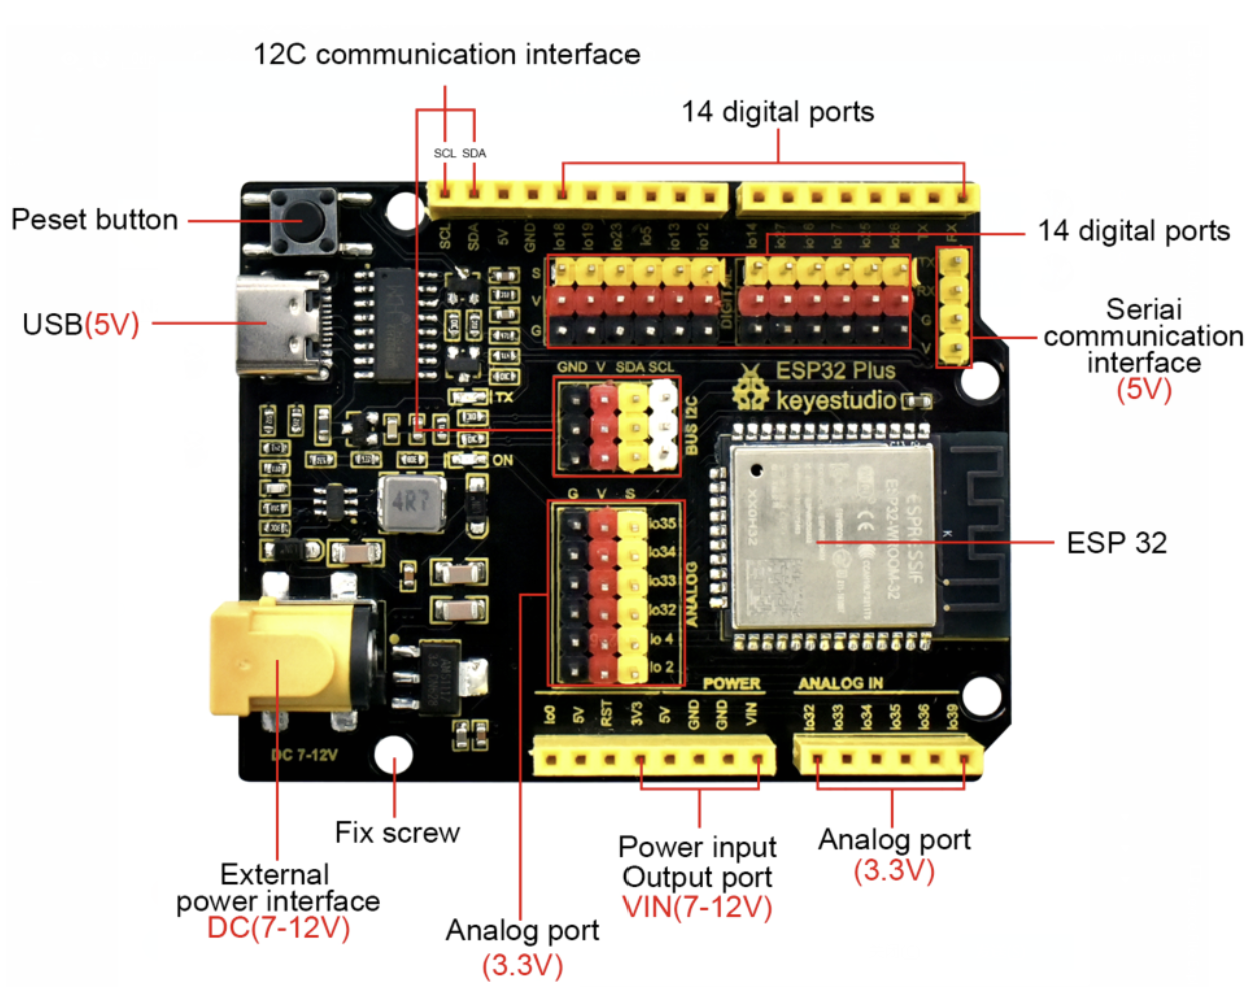
\includegraphics[width=\textwidth]{fig/fig22.png}
	\caption{ESP32 Plus pins}
\end{figure}
\clearpage
\section{Arduino IDE}
\subsection{Introduktion}
Arduino IDE er et open-source værktøj, der bruges til at skrive og uploade kode til Arduino boards. Det understøtter mange forskellige Arduino boards og tilbyder en brugervenlig grænseflade til udvikling af embedded systemer.

\subsection{Installationstrin}
\begin{enumerate}
	\item Start med at downloade \textbf{Arduino IDE} fra \url{https://www.arduino.cc/en/software}. Vælg den version, der passer til dit operativsystem (Windows, macOS eller Linux).
	\item Følg installationsvejledningen på Arduino websitet for at installere Arduino IDE på din computer.
	\item Efter installationen, åbn Arduino IDE. Du skulle nu se en simpel teksteditor med flere funktioner og værktøjslinjer.
	\begin{figure}[!h]
		\centering
		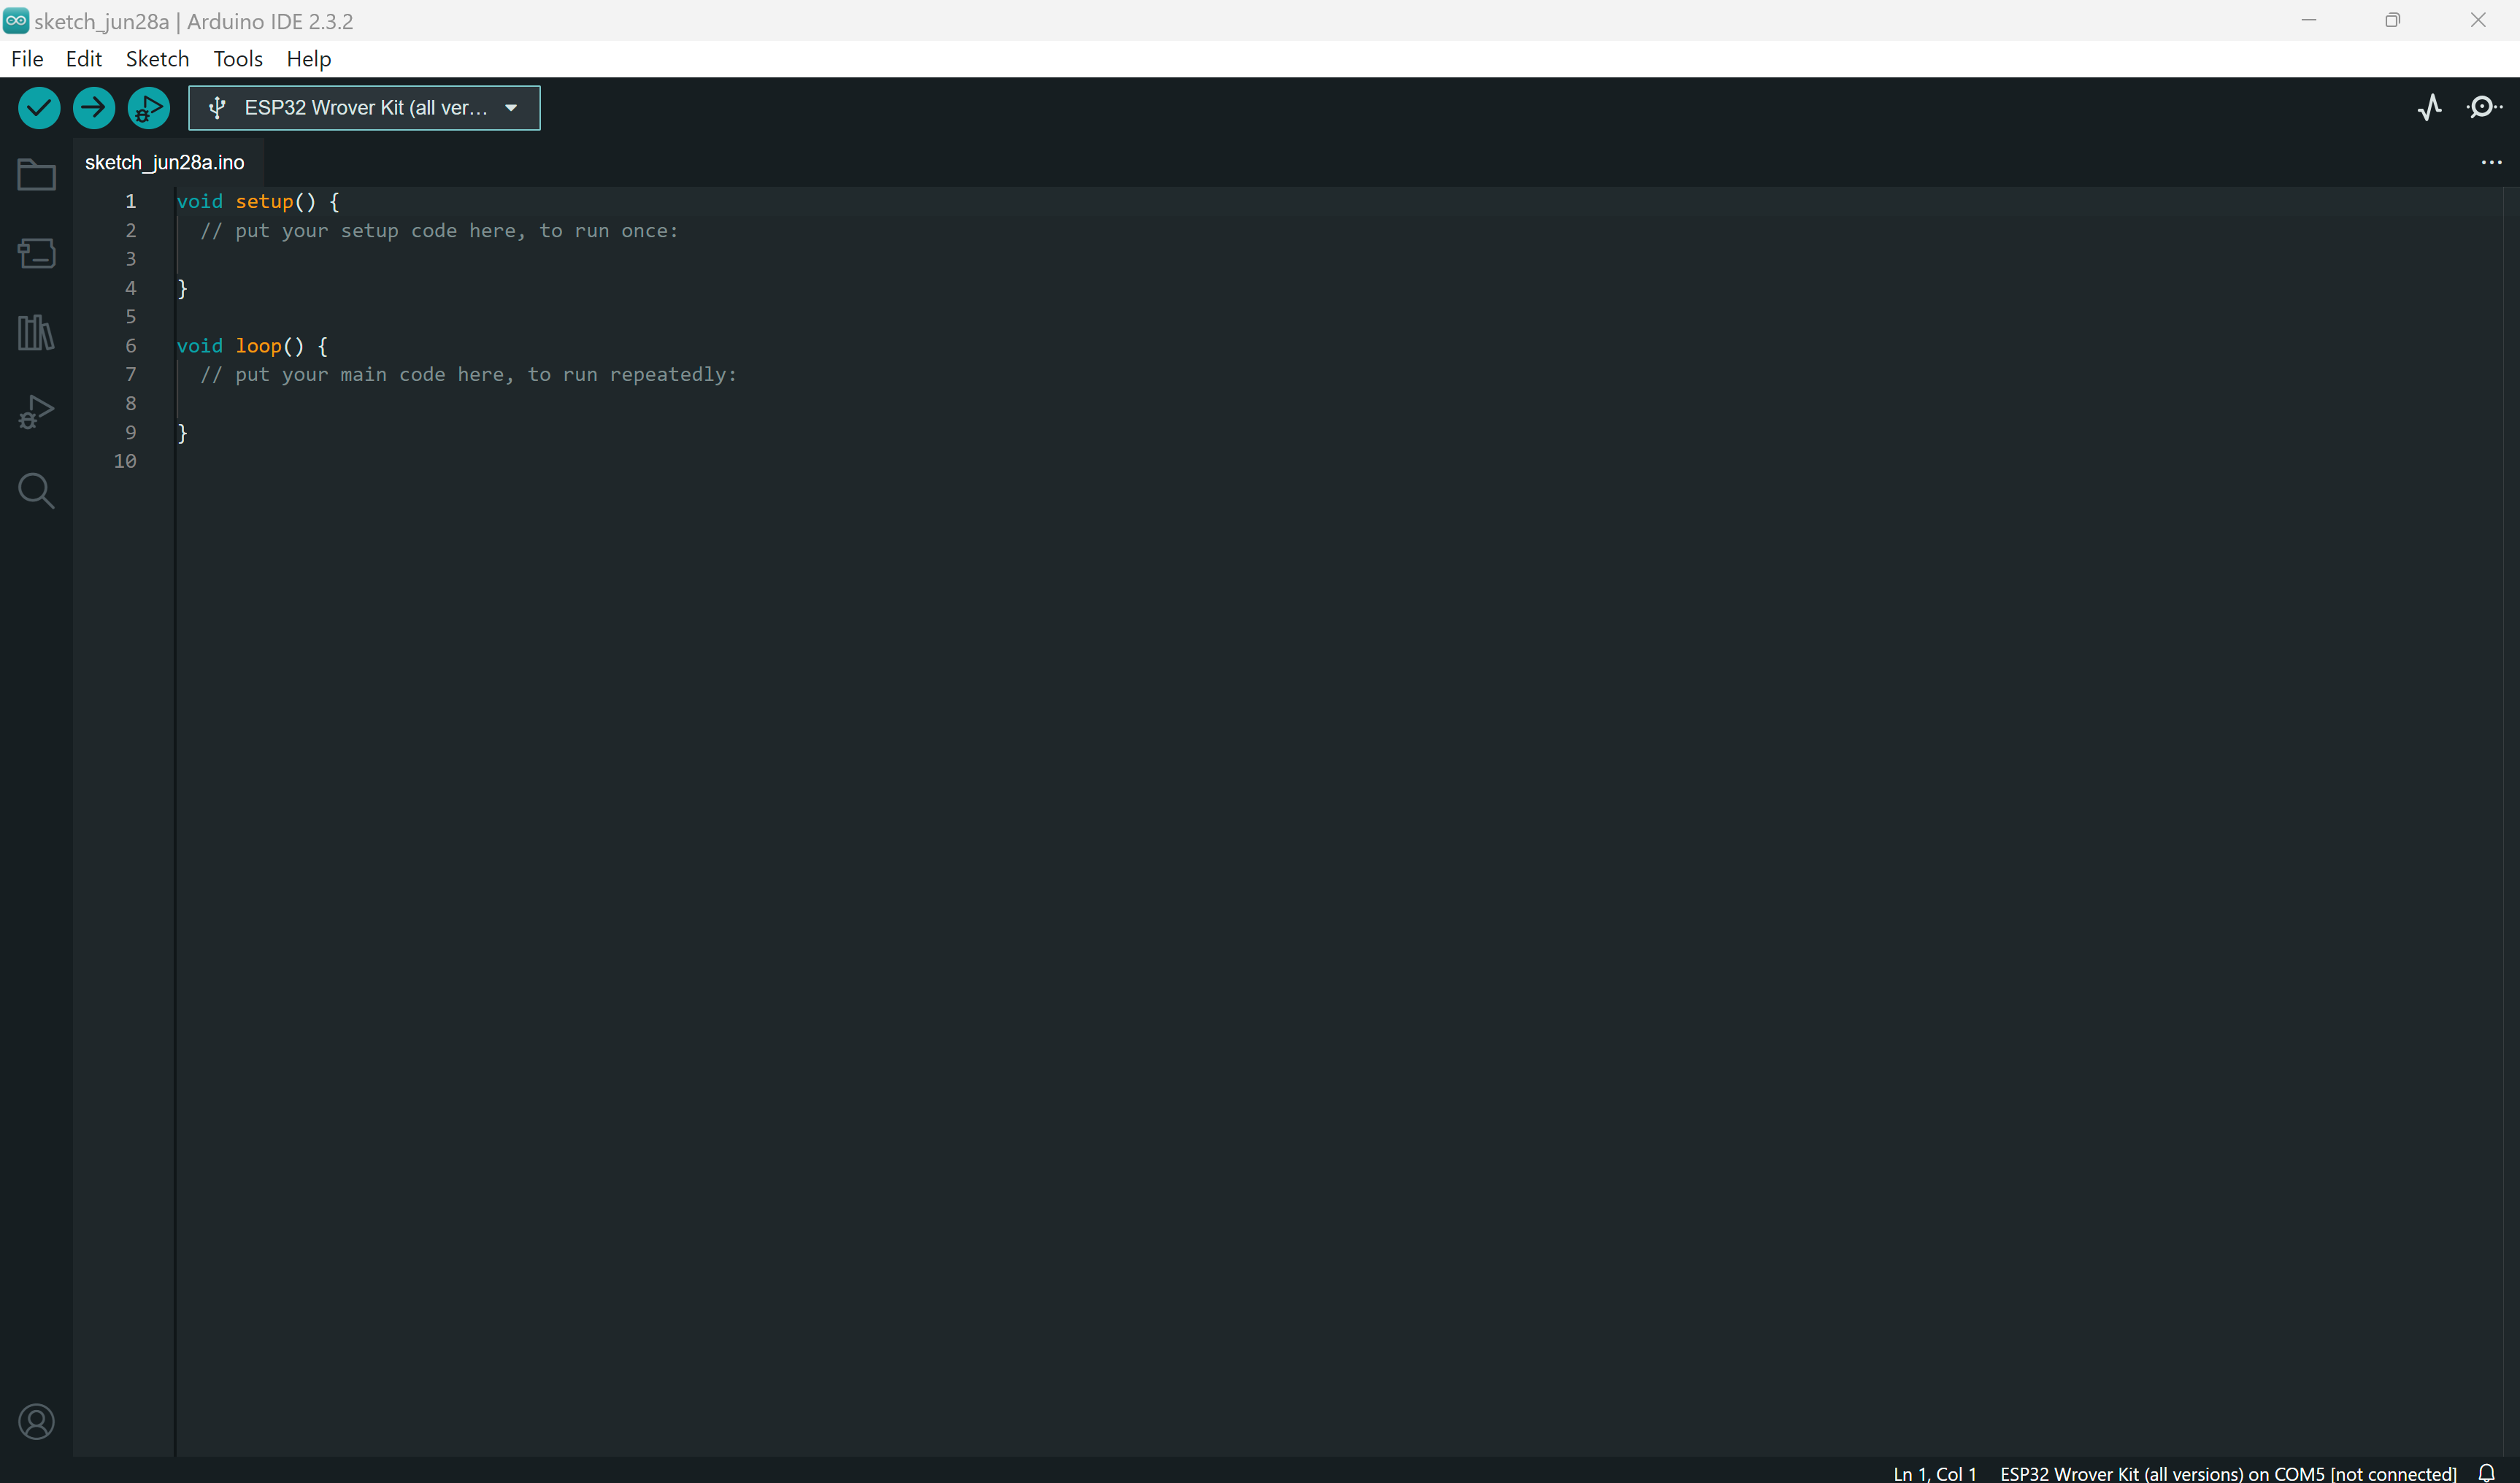
\includegraphics[width=\textwidth]{fig/fig23.png}
		\caption{Arduino IDE}
	\end{figure}
	\item Forbind dit Arduino board til din computer ved hjælp af et USB-kabel.
	\item I Arduino IDE, gå til \textit{Tools} menuen, vælg \textit{Board} og vælg det board, du bruger (f.eks. Arduino Uno).
	\item Gå derefter til \textit{Tools} menuen igen, vælg \textit{Port} og vælg den port, der svarer til dit tilsluttede Arduino board.
\end{enumerate}

\subsection{Oprettelse af et nyt projekt}
\begin{enumerate}[resume]
	\item Klik på \textit{File} menuen og vælg \textit{New} for at oprette et nyt projekt.
	\item Skriv din kode i editoren. Her er et simpelt eksempel:
	\begin{lstlisting}[language=C++]
		void setup() {
			// initialize digital pin LED_BUILTIN as an 
			//output.
			pinMode(LED_BUILTIN, OUTPUT);
		}
		
		void loop() {
			// turn the LED on (HIGH is the voltage level)
			digitalWrite(LED_BUILTIN, HIGH);
			// wait for a second
			delay(1000);
			// turn the LED off by making the voltage LOW
			digitalWrite(LED_BUILTIN, LOW);
			// wait for a second
			delay(1000);
		}
	\end{lstlisting}
	\item Klik på \textit{Upload} knappen (pilen) for at kompilere og uploade koden til dit Arduino board.
\end{enumerate}
%	C++ Basics
	\part{C++ Basics}
\chapter{C++}
\section{C++ }
\textbf{Formål:} Dette afsnit introducerer grundlæggende C++-begreber, som er essentielle for at programmere Arduino. Studerende vil lære om syntaks, output, kommentarer, variabler, brugerinput, datatyper, operatorer, strings, betingelser og loops. Disse emner danner grundlaget for at forstå mere avancerede koncepter og anvende dem i Arduino-projekter.
\newline\newline
\noindent\textbf{Læringsmål:} Efter at have læst dette afsnit forventes det, at studerende kan:
\begin{itemize}
	\item Forstå og skrive grundlæggende C++-syntaks.
	\item Udføre input og output operationer med Arduino.
	\item Bruge kommentarer til at dokumentere Arduino-kode.
	\item Deklarere og anvende variabler i Arduino-programmer.
	\item Modtage brugerinput fra Arduino-sensorer og behandle det.
	\item Identificere og anvende forskellige datatyper i Arduino-programmer.
	\item Anvende operatorer til forskellige operationer på Arduino.
	\item Håndtere strings effektivt i Arduino-kode.
	\item Skrive og forstå betingede udsagn (if-else) i Arduino-programmer.
	\item Implementere loops (while og for) for gentagne opgaver på Arduino.
\end{itemize}

\section{C++ Syntax}
\textbf{Teori:} C++ syntaks refererer til de regler og strukturer, der definerer hvordan man skriver et gyldigt C++ program. I Arduino IDE skrives C++ kode for at styre mikrocontrollerens funktioner. Et typisk Arduino-program består af to centrale funktioner:
\begin{itemize}
	\item \textbf{\texttt{setup()}}: Kører én gang, når Arduino'en starter. Bruges til initialisering.
	\item \textbf{\texttt{loop()}}: Kører kontinuerligt, efter \texttt{setup()} er udført. Bruges til hovedlogikken.
\end{itemize}
Disse funktioner definerer programflowet og strukturen i et Arduino-program.
\newline\newline
\noindent\textbf{Eksempel:}
\begin{lstlisting}[language=C++]
	void setup() {
		// initial setup code
		pinMode(13, OUTPUT); // Set pin 13 as output
	}
	
	void loop() {
		// repeated execution code
		digitalWrite(13, HIGH); // Turn on the LED
		delay(1000); // Wait for 1 second
		digitalWrite(13, LOW); // Turn off the LED
		delay(1000); // Wait for 1 second
	}
\end{lstlisting}
\begin{figure}[h!]
	\centering
	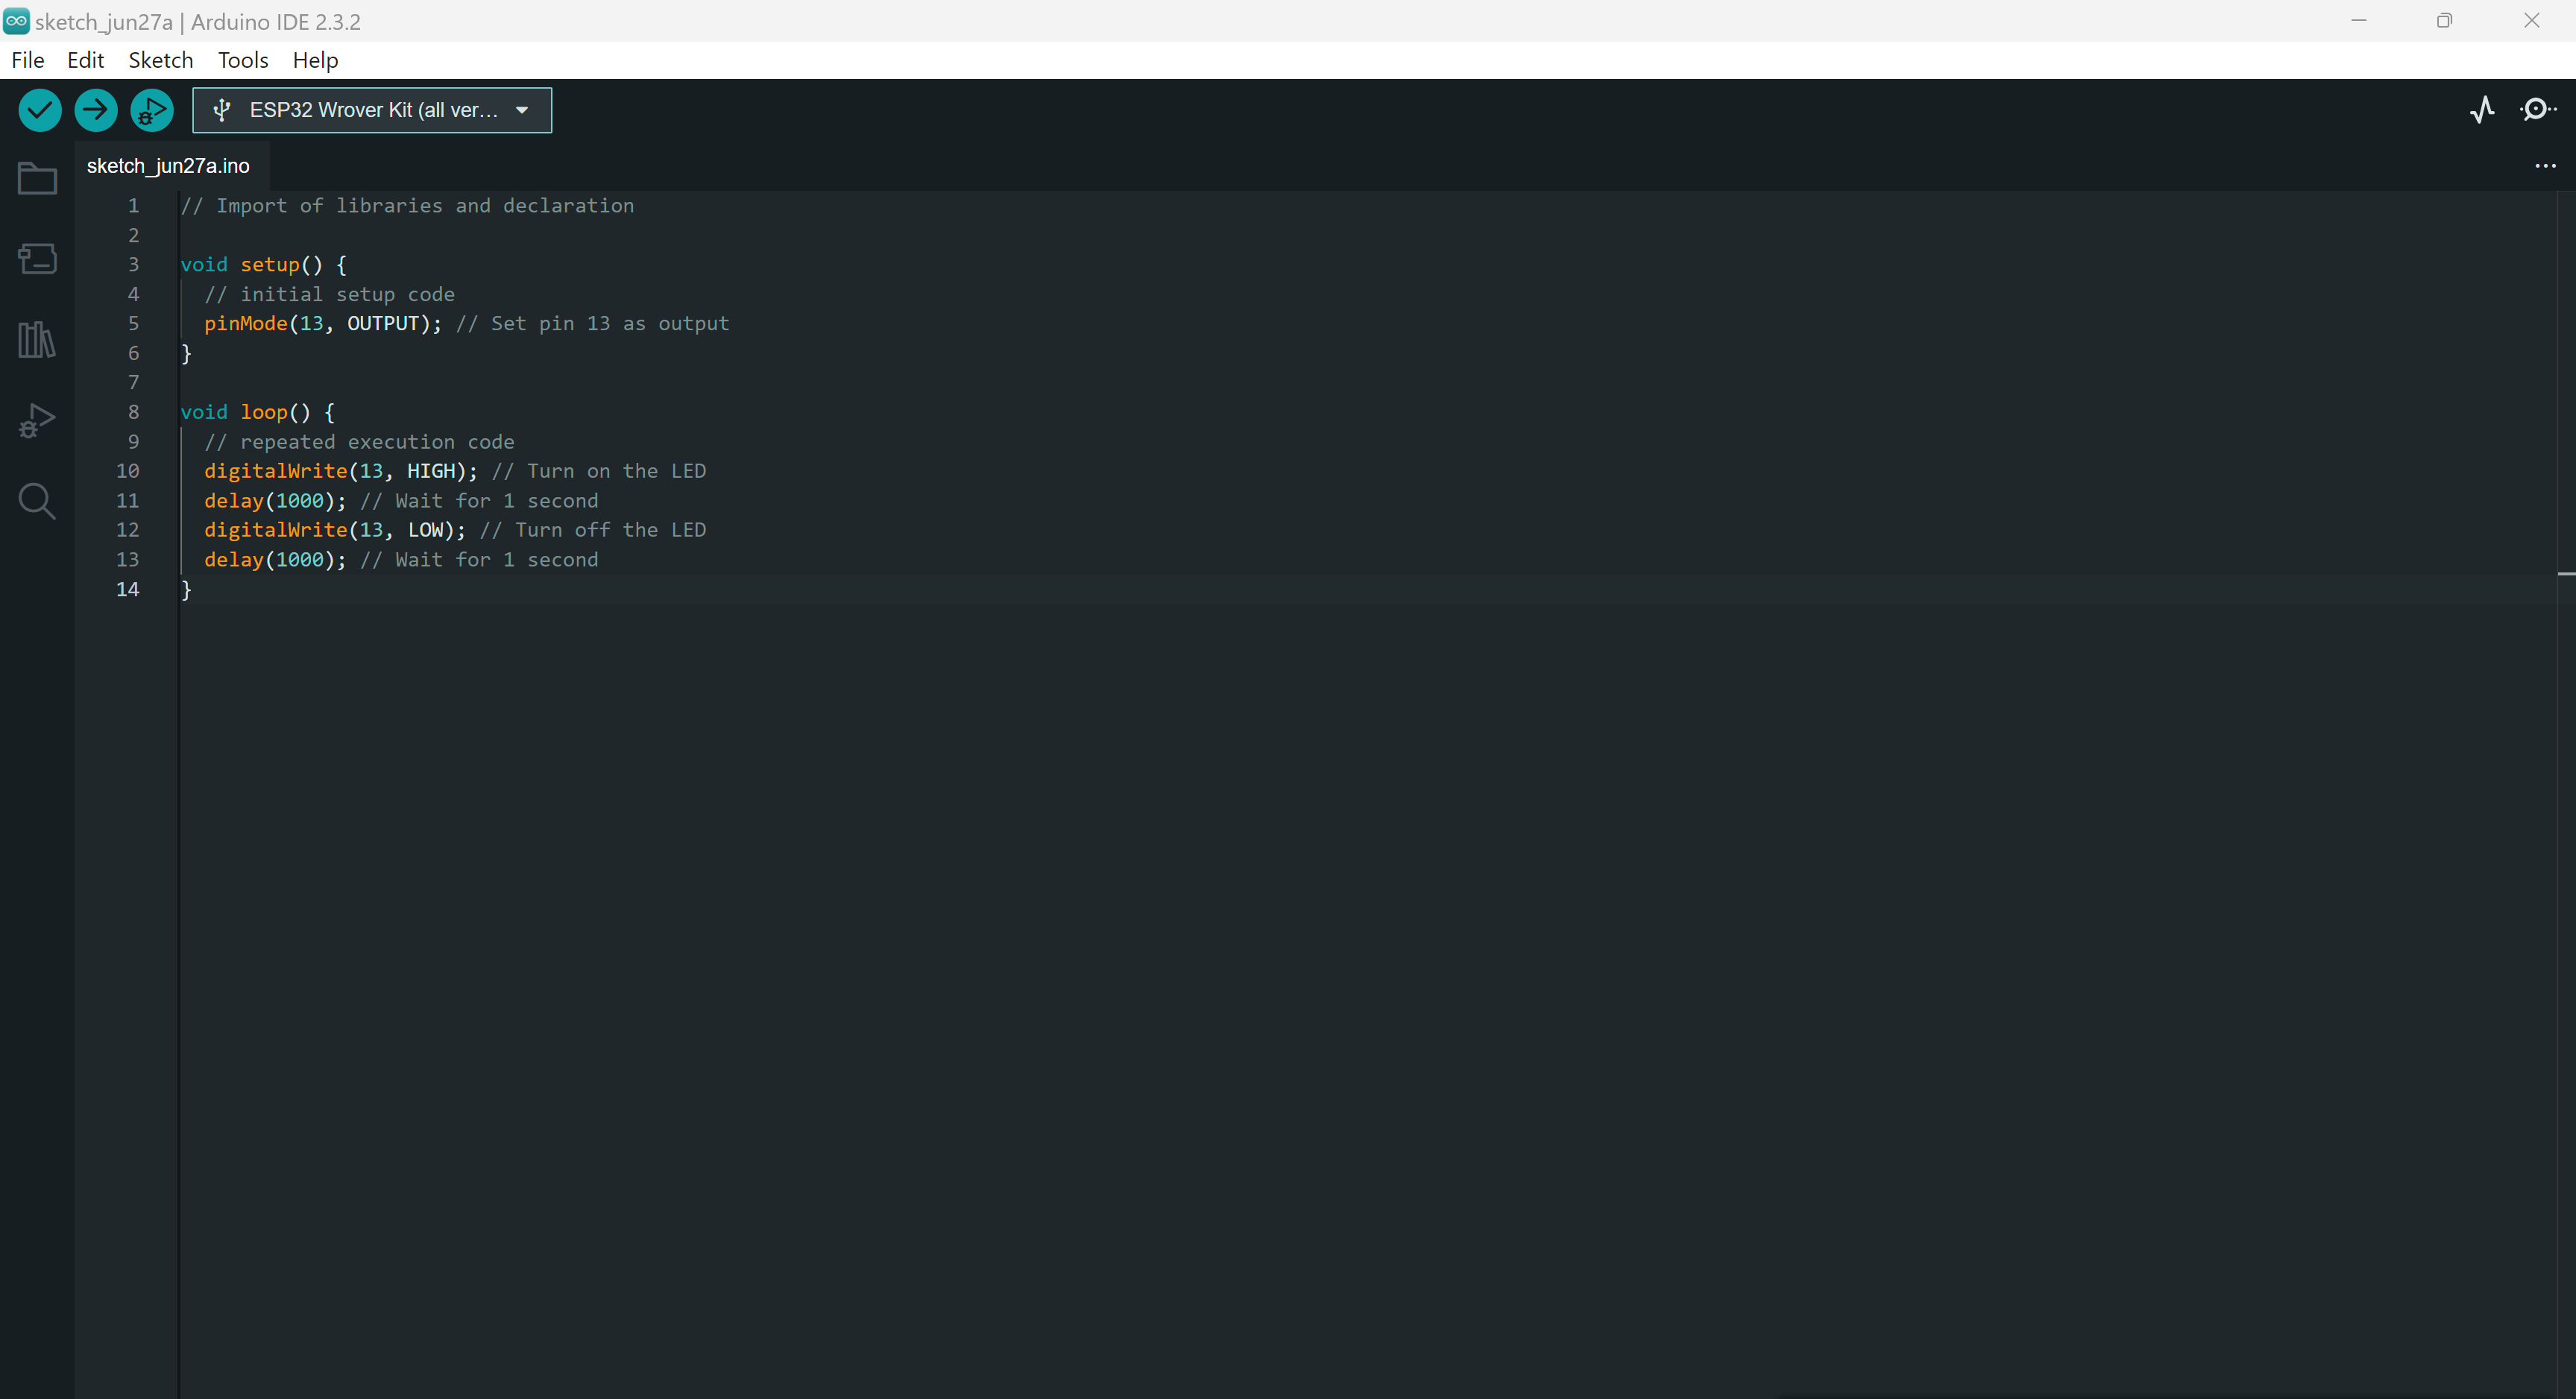
\includegraphics[width=\textwidth]{fig/fig19.png}
	\caption{C++ Syntax}
	\label{fig:19}
\end{figure}


\section{C++ Output}
\textbf{Teori:} Output i Arduino opnås ved at bruge \texttt{Serial.print()} og \texttt{Serial.println()} til at sende data til serial monitoren. Serial kommunikation er en vigtig funktion, som gør det muligt at kommunikere mellem Arduino og en computer. Dette er især nyttigt til debugging og overvågning af sensorværdier.
\newline\newline
\noindent\textbf{Serial Monitor:} Serial Monitor er et værktøj i Arduino IDE (Integrated Development Environment), der giver brugeren mulighed for at interagere med Arduino-boardet via seriel kommunikation. Når en Arduino er tilsluttet en computer via USB-kabel, kan den sende og modtage data til og fra computeren. Serial Monitor viser disse data i et tekstvindue og giver brugeren mulighed for at sende tekstdata til Arduinoen.
\newline\newline
\noindent Serial Monitor bruges ofte til følgende formål:
\begin{itemize}
	\item \textbf{Debugging:} Ved at bruge \texttt{Serial.print()} og \texttt{Serial.println()} kan programmører indsætte debugging-meddelelser i deres kode for at overvåge, hvad der sker i programmet. Dette gør det lettere at identificere og rette fejl.
	
	\item \textbf{Overvågning af sensorværdier:} Arduino kan læse data fra forskellige sensorer (f.eks. temperatur, lys, fugtighed) og sende disse data til Serial Monitor for at give en realtidsvisning af sensorens output.
	
	\item \textbf{Brugerinput:} Brugere kan sende kommandoer eller data fra Serial Monitor til Arduino. Dette er nyttigt til at ændre parametre i programmet uden at skulle uploade ny kode til Arduinoen.
	
	\item \textbf{Kommunikation:} Serial Monitor kan bruges til at kommunikere med andre serielle enheder, som er tilsluttet Arduinoen, såsom GPS-moduler, GSM-moduler, og andre mikrocontrollere.
\end{itemize}
\noindent\textbf{Eksempel: Output til Seriel Monitor}
\begin{lstlisting}[language=C++]
	void setup() {
		Serial.begin(9600); // Initialize serial communication at 9600 baud
	}
	
	void loop() {
		Serial.println("Hello, Arduino!");
		delay(1000); // wait for a second
	}
\end{lstlisting}
\clearpage
\begin{figure}[h!]
	\centering
	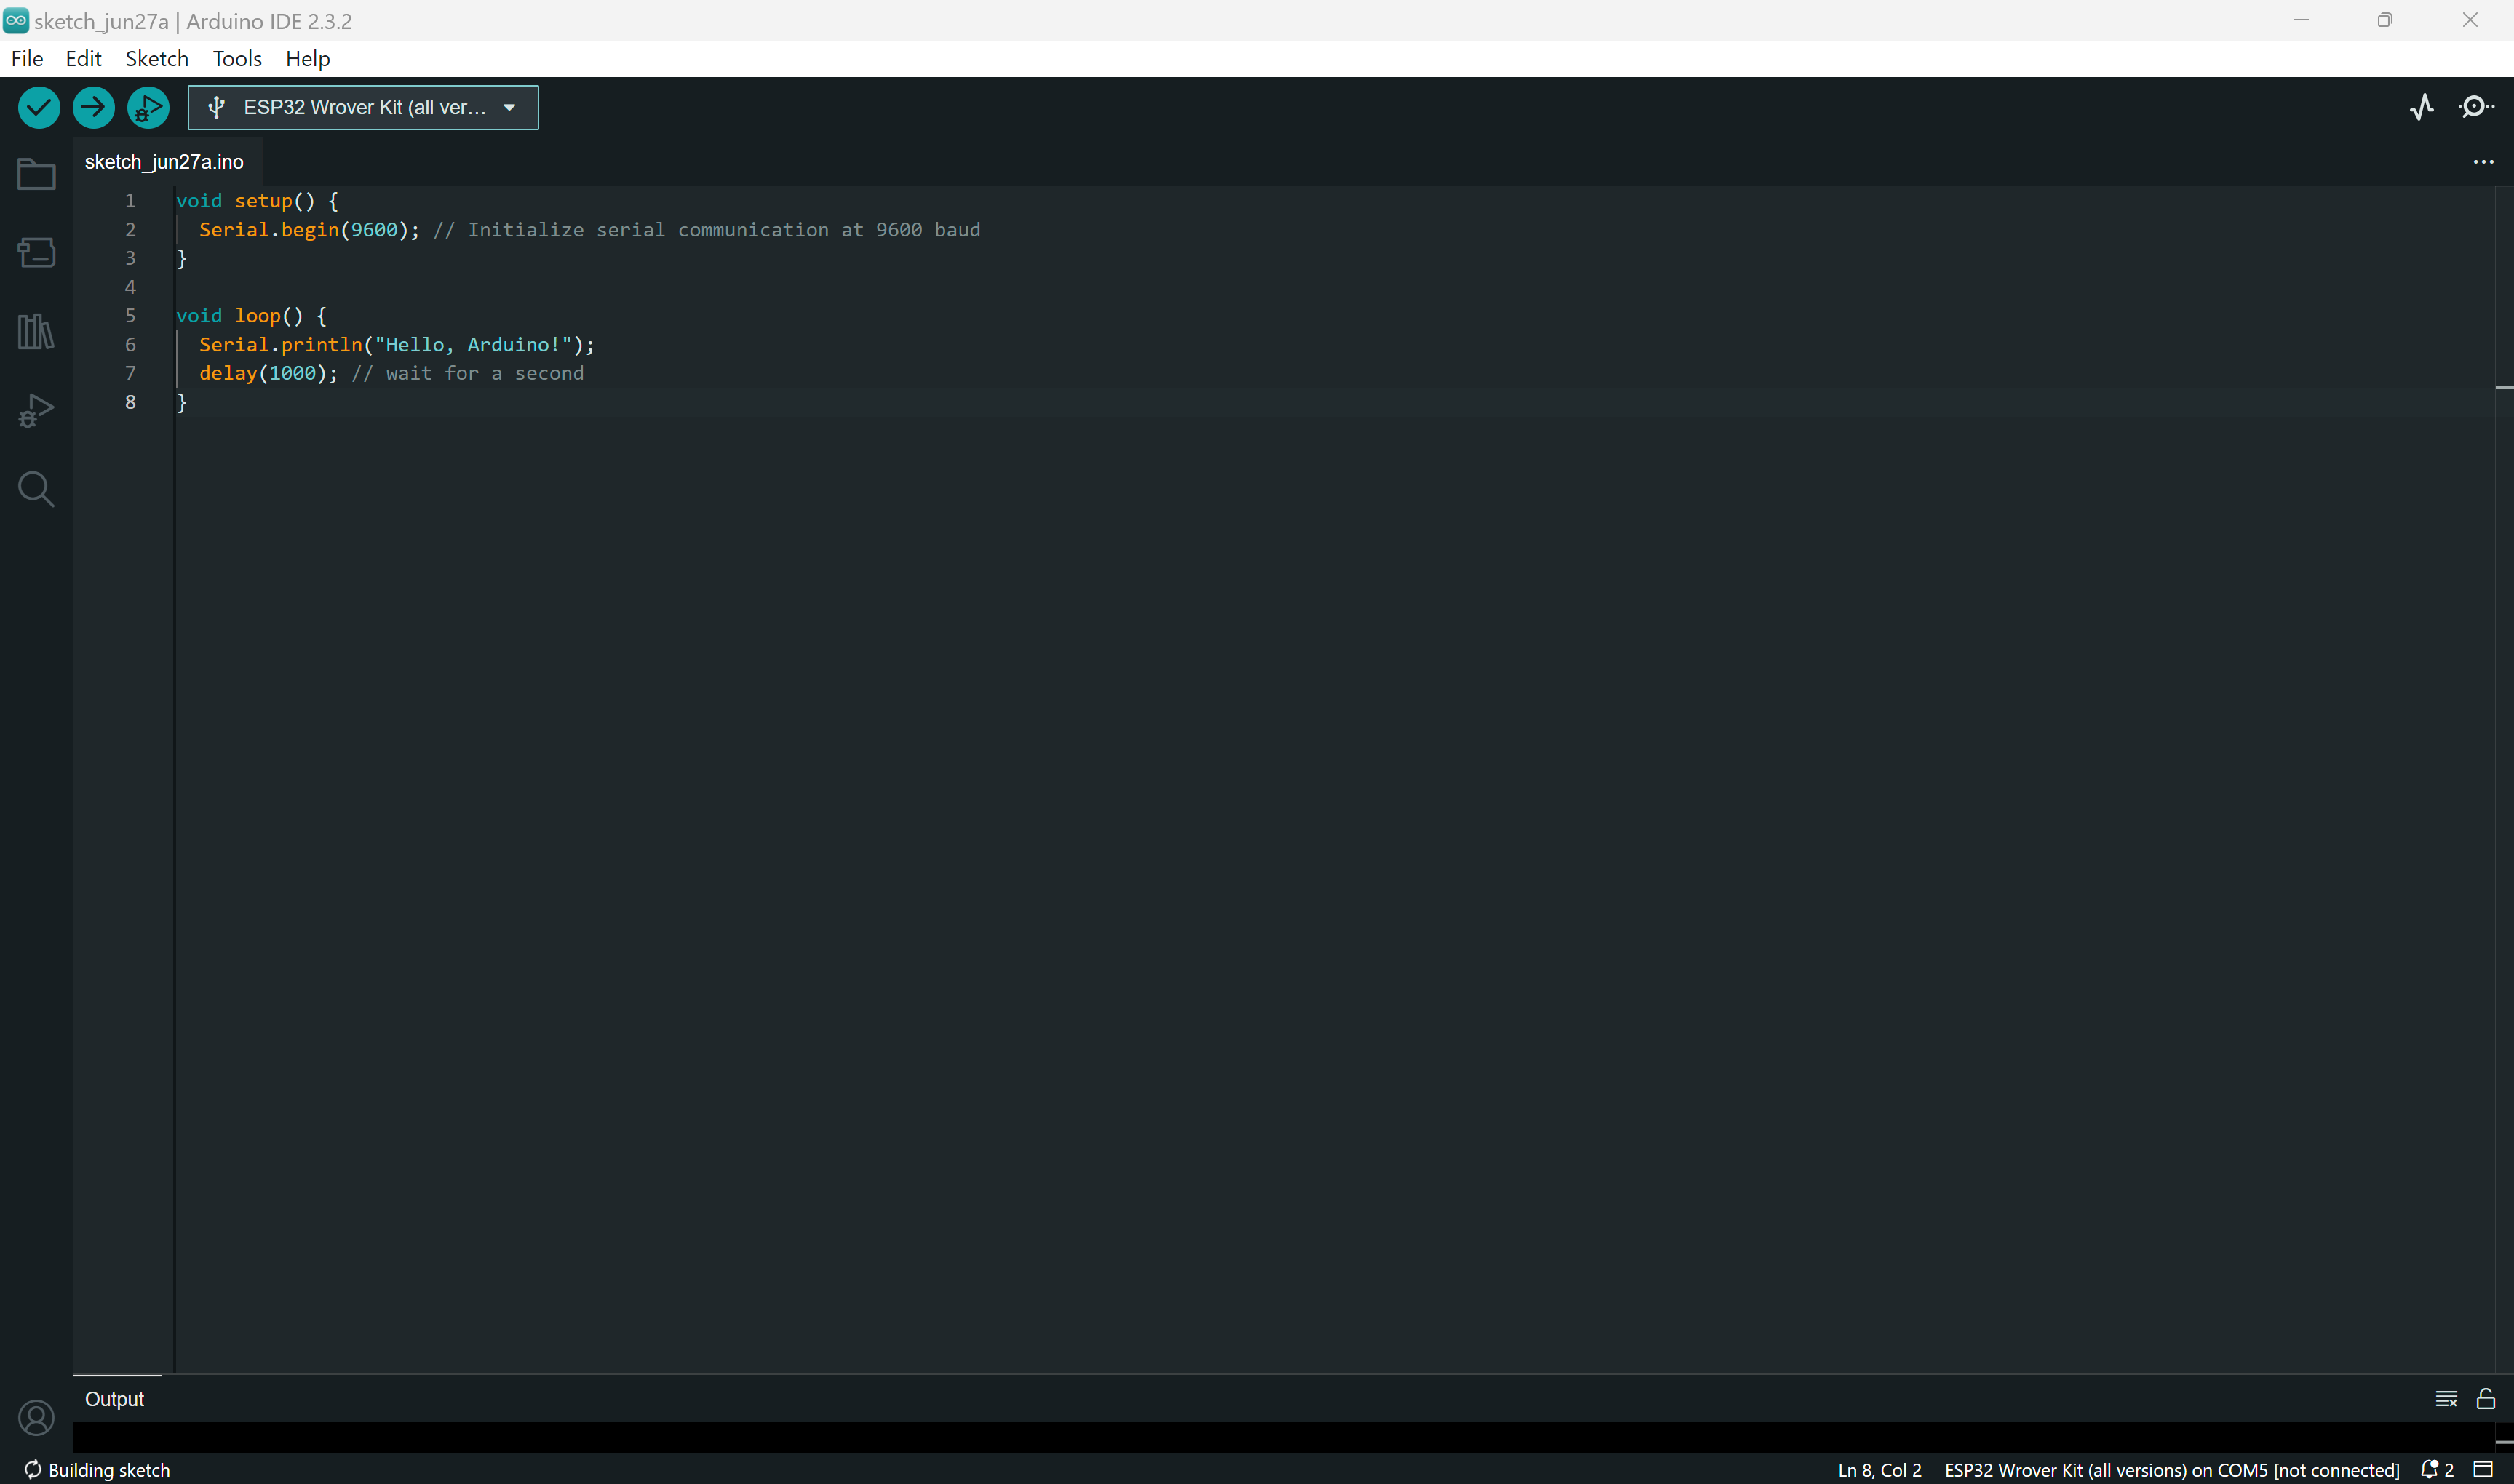
\includegraphics[width=\textwidth]{fig/fig1.png}
	\caption{C++ Output}
	\label{fig:1}
\end{figure}

\noindent\textbf{Eksempel: Seriel Monitor for debugging}
\begin{lstlisting}[language=C++]
	void setup() {
		Serial.begin(9600); // Initialize serial communication at 9600 baud
	}
	
	void loop() {
		int sensorValue = analogRead(A0);
		Serial.print("Sensor Value: ");
		Serial.println(sensorValue);
	}
\end{lstlisting}
\clearpage
\begin{figure}[h!]
	\centering
	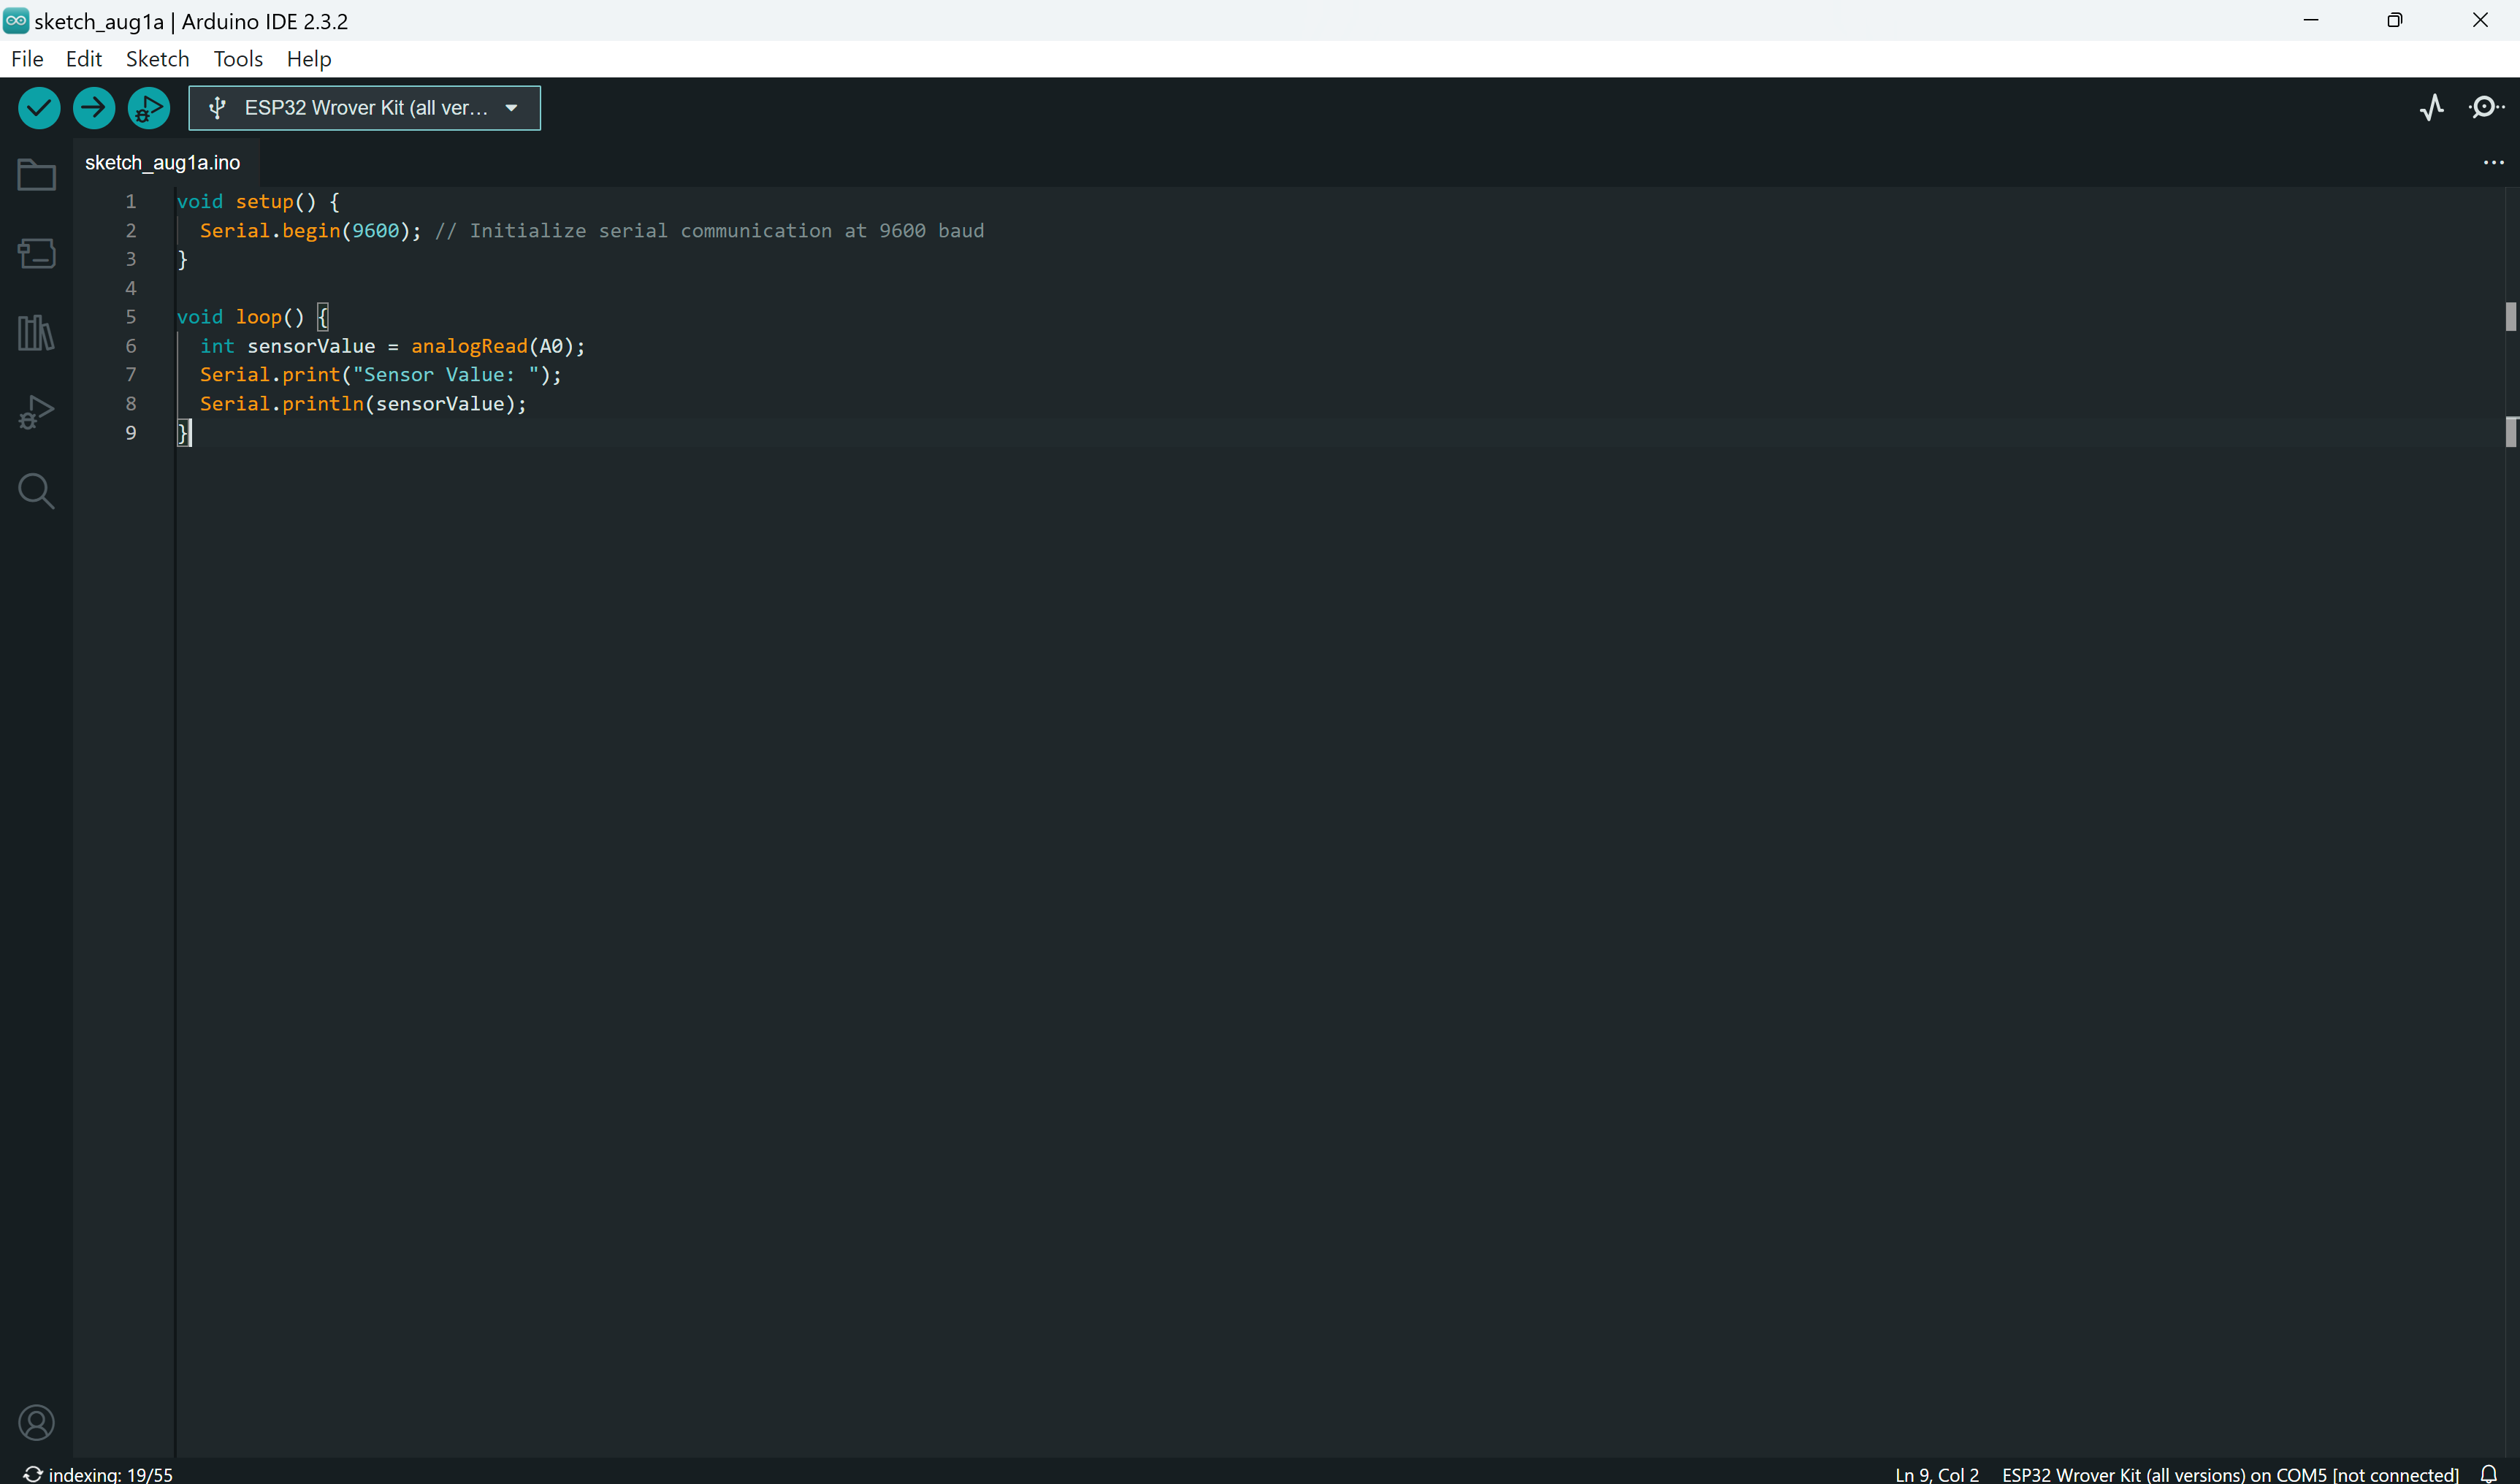
\includegraphics[width=\textwidth]{fig/fig21.png}
	\caption{C++ Output}
	\label{fig:21}
\end{figure}

\section{C++ Comments}
\textbf{Teori:} Kommentarer bruges til at dokumentere koden og forklare, hvad de forskellige dele af programmet gør. De ignoreres af compileren og gør det lettere for andre (og dig selv) at forstå koden senere.
\begin{itemize}
	\item Hvis \texttt{//} bruges, så laves en kommentar for en enkelt linje.
	\item Hvis \texttt{/* */} bruges, vil alt imellem \texttt{/*} og \texttt{*/} blive betragtet som en kommentar.
\end{itemize}
Udover at blive brugt til at lave kommentarer, kan de også bruges til at debugge koden ved midlertidigt at deaktivere visse dele af programmet.
\clearpage
\noindent\textbf{Eksempel:}
\begin{lstlisting}[language=C++]
	// This is a single line comment
	/*
	This is a block comment
	that spans multiple lines
	*/
	void setup() {
		// Initialize pin 13 as an output
		pinMode(13, OUTPUT);
	}
\end{lstlisting}
\begin{figure}[h!]
	\centering
	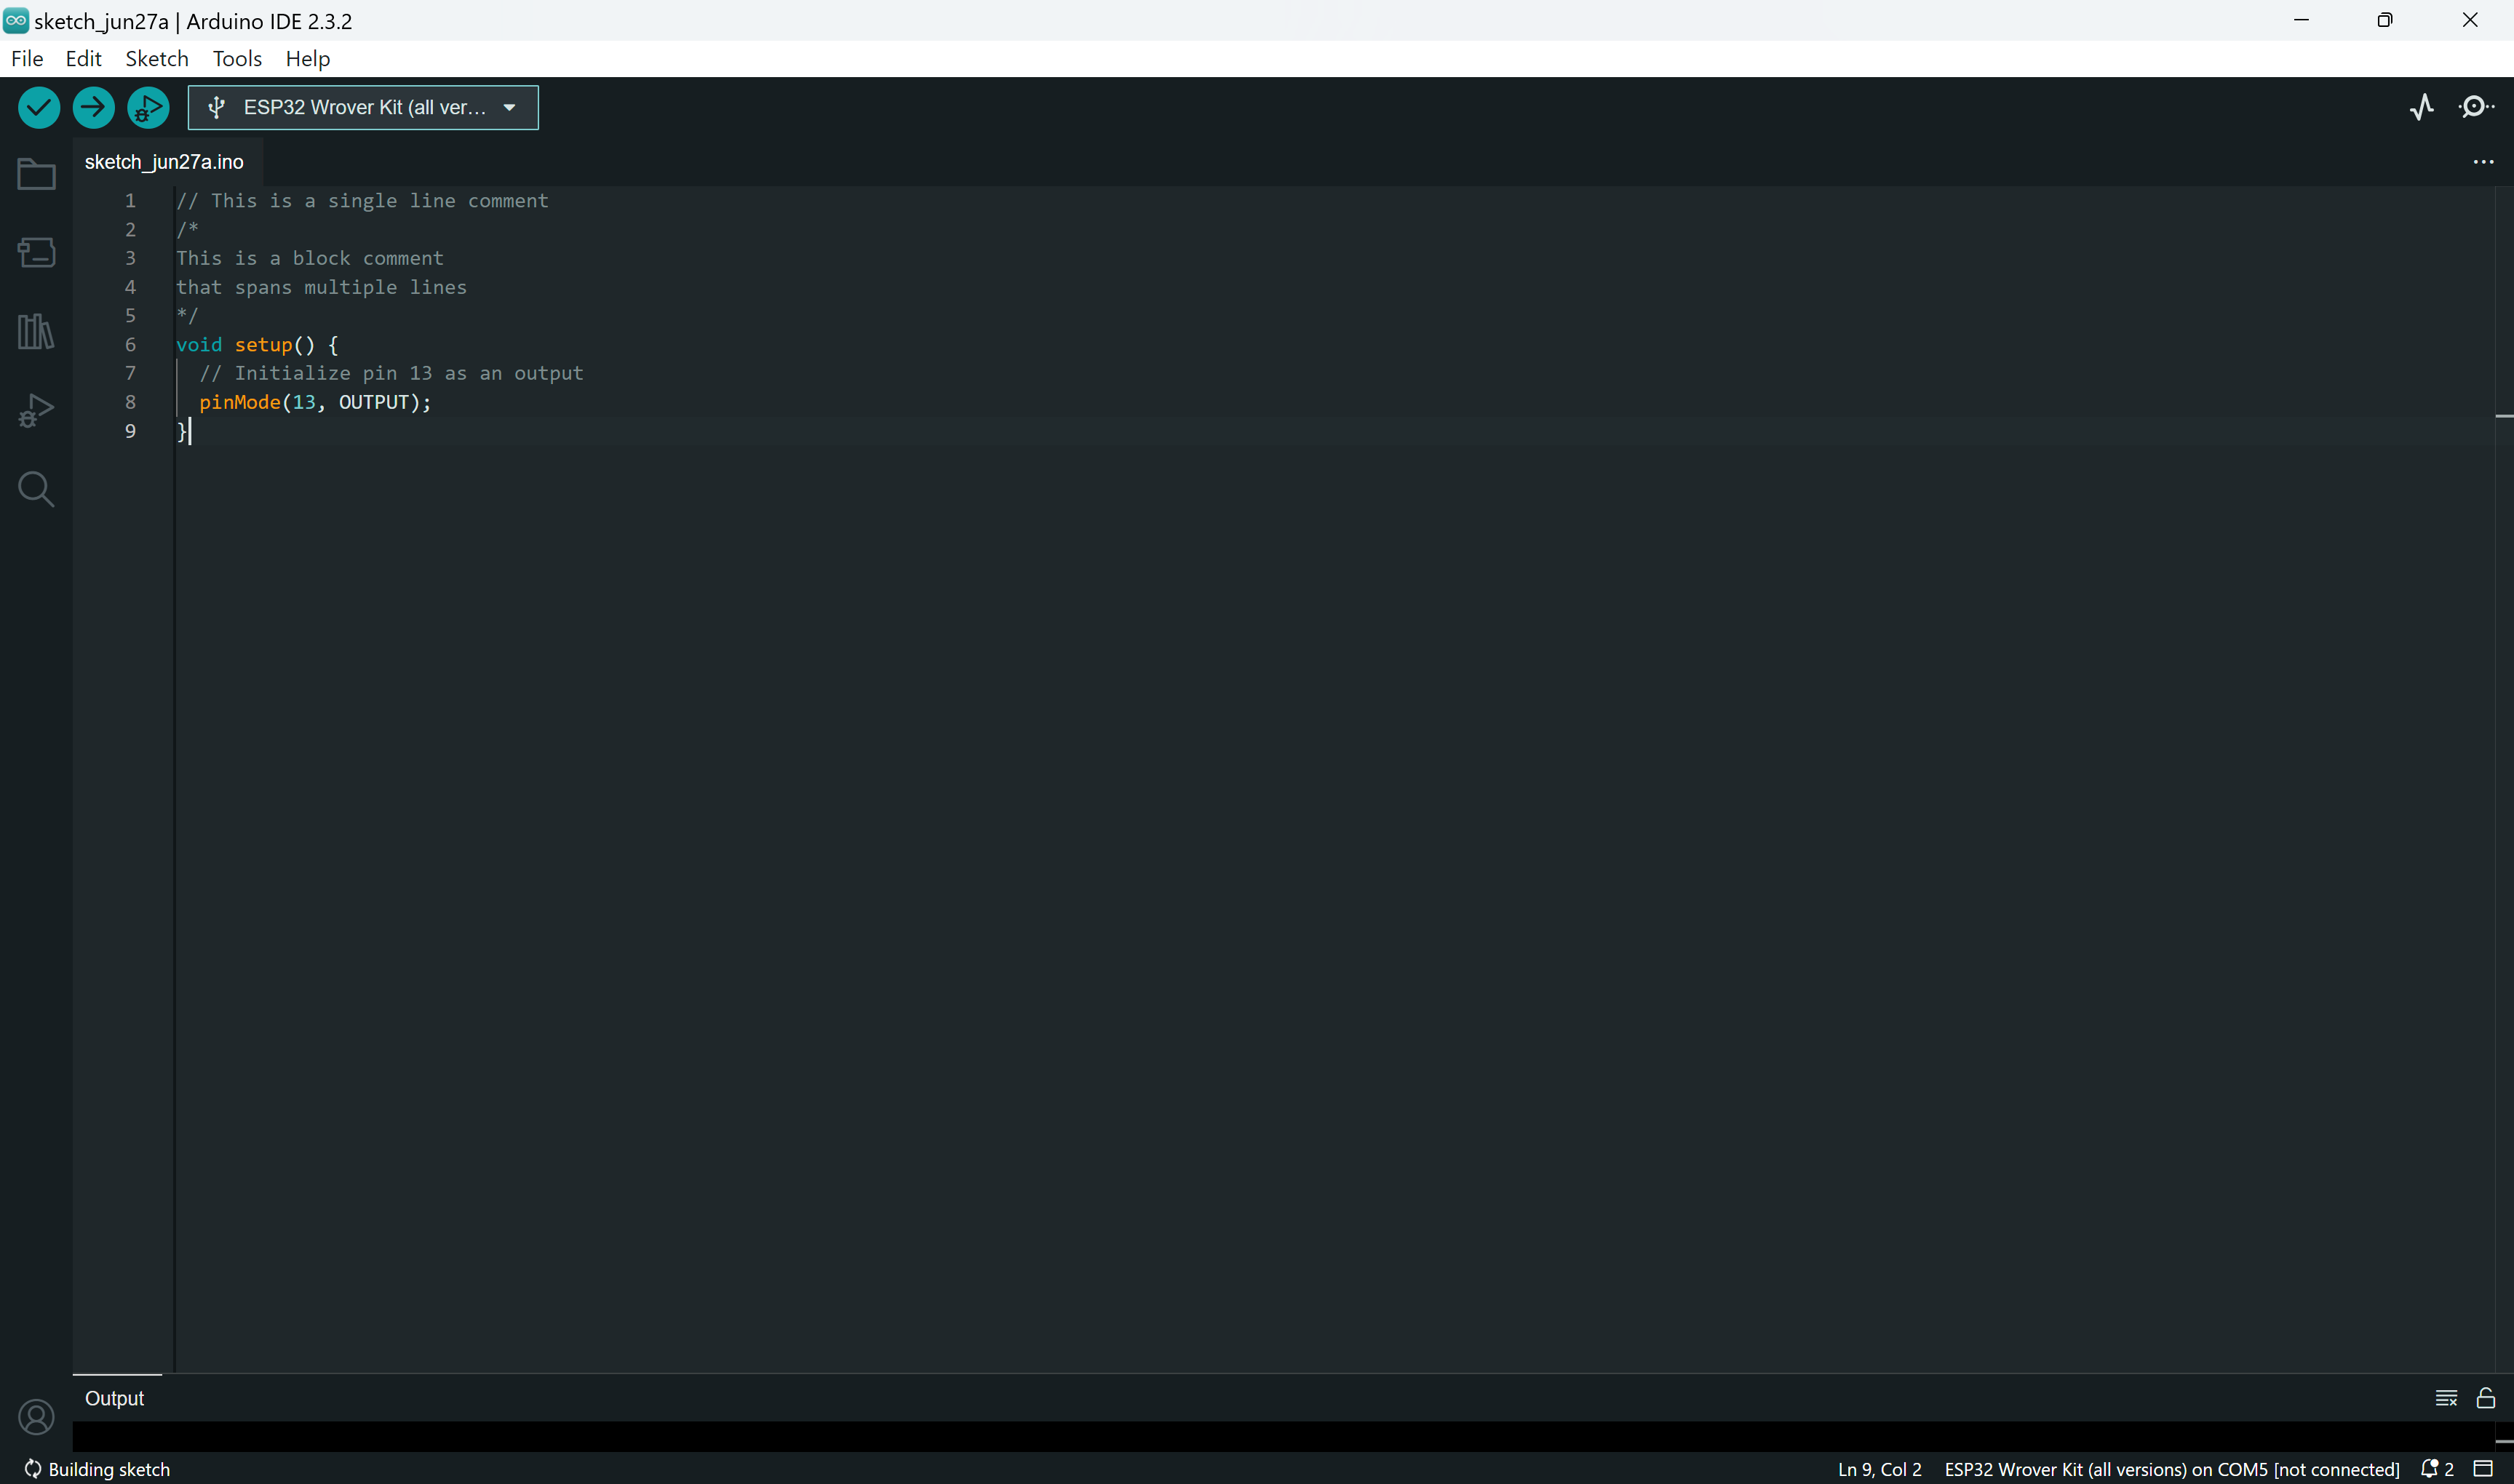
\includegraphics[width=\textwidth]{fig/fig2.png}
	\caption{C++ Comments}
	\label{fig:2}
\end{figure}

\section{C++ Variables}
\textbf{Teori:} Variabler bruges til at gemme data, der kan ændres under programmets kørsel. Variabler skal deklareres med en datatype før brug. Typiske datatyper inkluderer \texttt{int}, \texttt{float}, \texttt{char}, og \texttt{bool}.
\clearpage
\noindent\textbf{Eksempel:}
\begin{lstlisting}[language=C++]
	int ledPin = 13; // declare an integer variable
	
	void setup() {
		pinMode(ledPin, OUTPUT); // use the variable
	}
	
	void loop() {
		digitalWrite(ledPin, HIGH); // turn the LED on
		delay(1000);
		digitalWrite(ledPin, LOW); // turn the LED off
		delay(1000);
	}
\end{lstlisting}
\begin{figure}[h!]
	\centering
	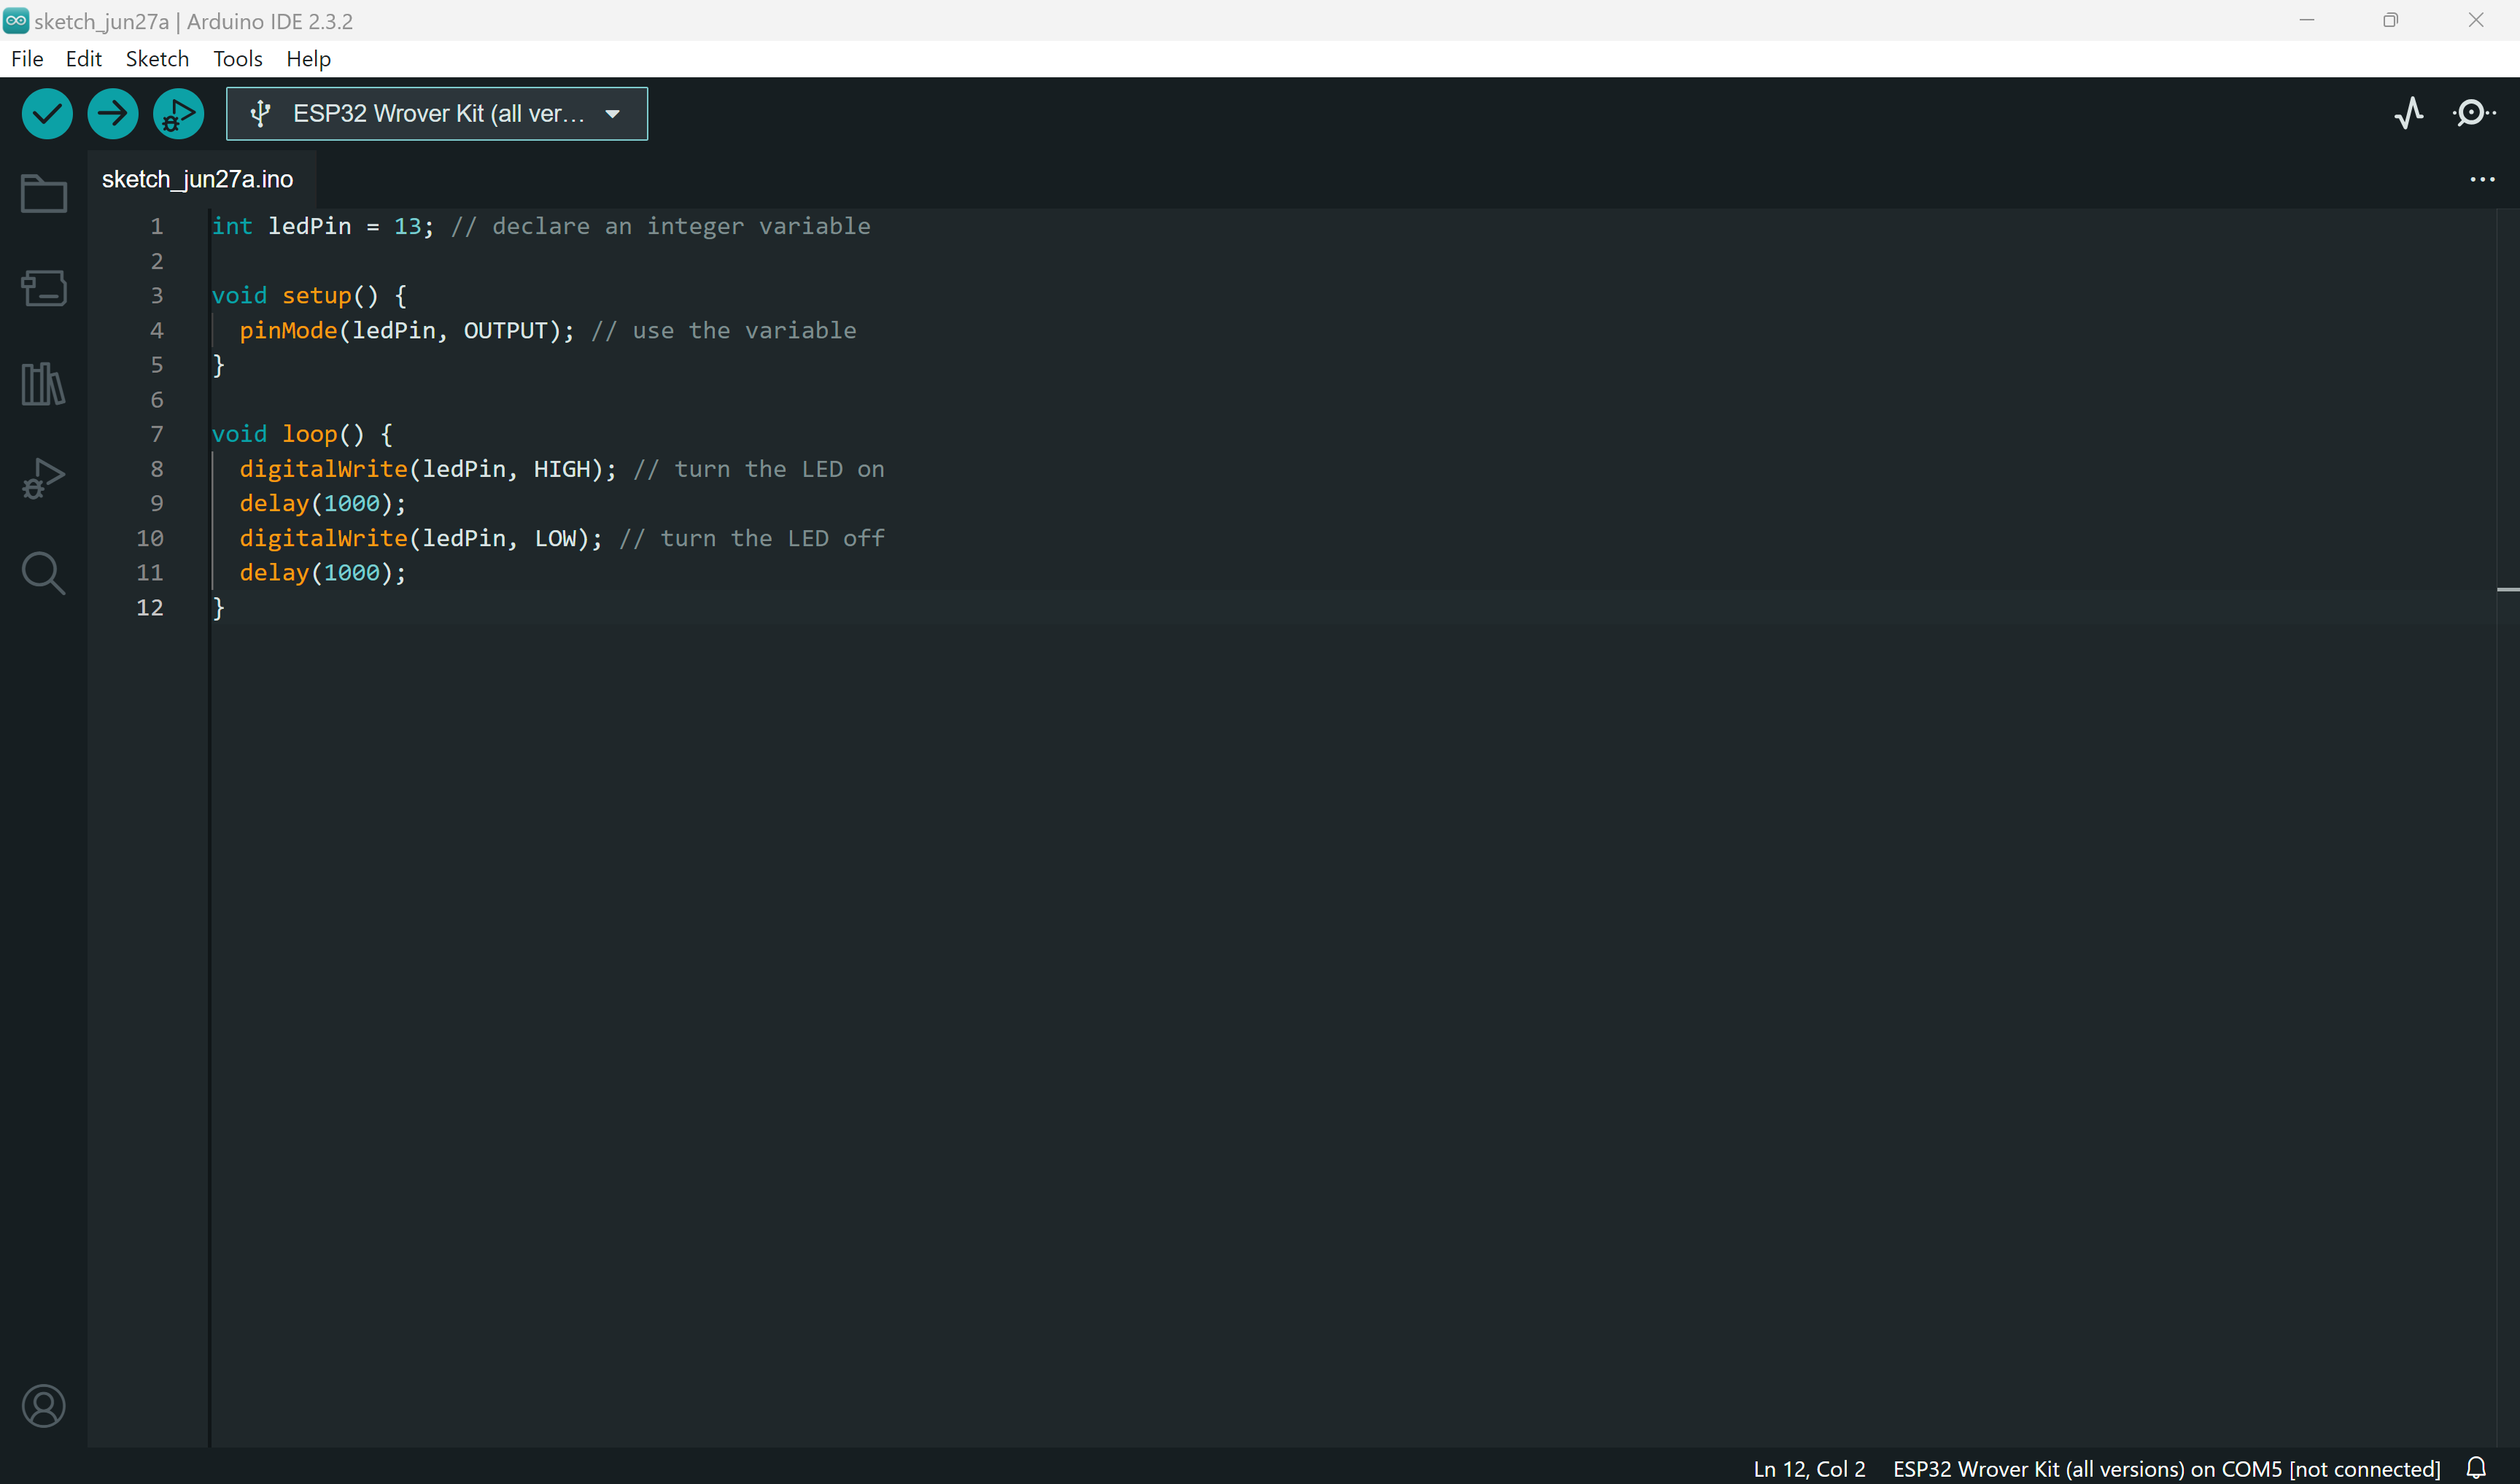
\includegraphics[width=\textwidth]{fig/fig3.png}
	\caption{C++ Variables}
	\label{fig:3}
\end{figure}

\noindent\textbf{Navnekonventioner for Variabler}
Når man skriver kode, er det vigtigt at følge nogle navnekonventioner for variabler for at gøre koden læsbar og nemmere at vedligeholde. Her er nogle almindelige navnekonventioner:
\begin{itemize}
	\item \textbf{camelCase}: Begynder med et lille bogstav, og hvert efterfølgende ord starter med et stort bogstav. Eksempel: \texttt{sensorValue}, \texttt{scaledValue}.
	\item \textbf{PascalCase}: Hvert ord starter med et stort bogstav. \\Eksempel: \texttt{SensorValue}, 
	\texttt{ScaledValue}.
	\item \textbf{snake\_case}: Alle bogstaver er små, og ord adskilles med underscores. Eksempel: 
	\texttt{sensor\_value}, \texttt{scaled\_value}.
	\item \textbf{kebab-case}: Alle bogstaver er små, og ord adskilles med bindestreger (bruges sjældent i programmeringssprog som C++). \\Eksempel:
	\texttt{sensor-value}, \texttt{scaled-value}.
\end{itemize}

\section{C++ User Input}
\textbf{Teori:} Brugerinput modtages via sensorer eller knapper og behandles med \texttt{analogRead()} og \texttt{digitalRead()} funktioner. Disse funktioner gør det muligt for Arduino at interagere med omgivelserne. \texttt{analogRead(pin)} læser en værdi mellem 0 og 1023 fra en analog pin, mens \texttt{digitalRead(pin)} læser enten HIGH eller LOW fra en digital pin.
\newline\newline
\noindent\textbf{Eksempel:}
\begin{lstlisting}[language=C++]
	int sensorPin = A0; // select the input pin for the sensor
	int sensorValue = 0; // variable to store the value coming from the sensor
	
	void setup() {
		Serial.begin(9600); // initialize serial communication
	}
	
	void loop() {
		sensorValue = analogRead(sensorPin); // read the value from the sensor
		Serial.println(sensorValue); // print the value to the serial monitor
		delay(1000); // wait for a second
	}
\end{lstlisting}
\clearpage
\begin{figure}[t!]
	\centering
	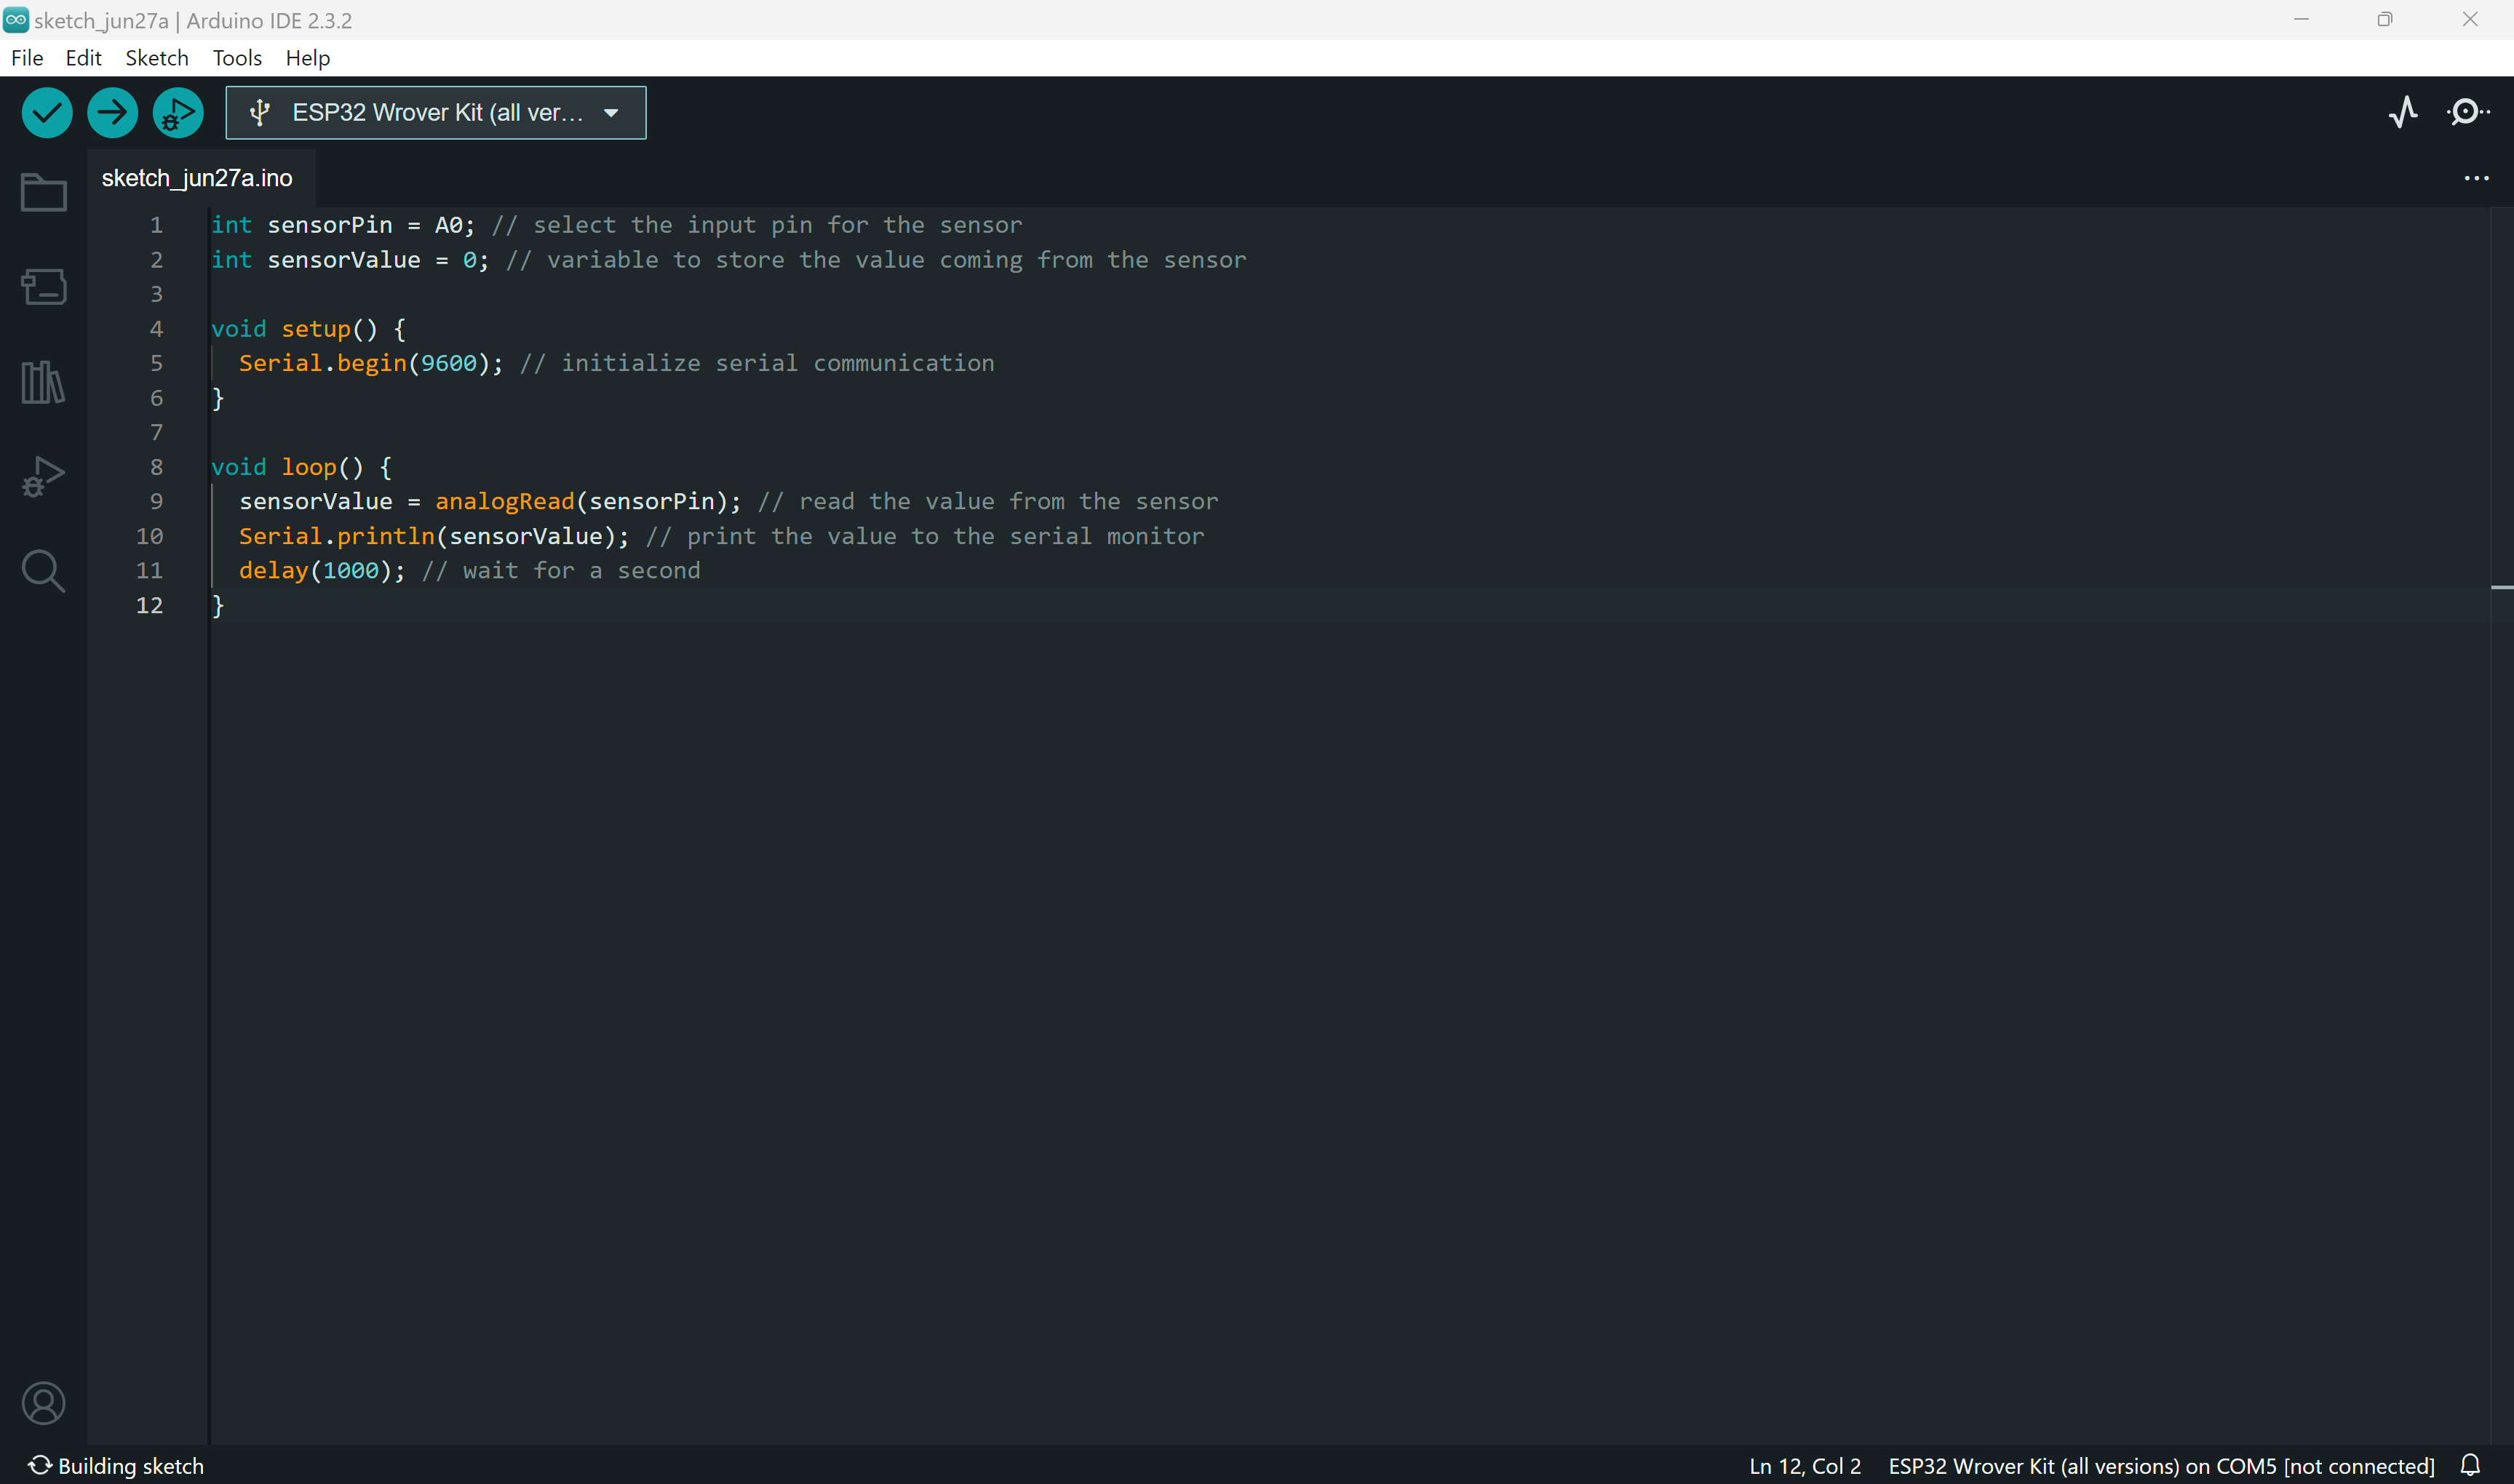
\includegraphics[width=\textwidth]{fig/fig4.png}
	\caption{C++ User Input}
	\label{fig:4}
\end{figure}
\section{C++ Data Types}
\textbf{Teori:} Data typer i C++ definerer den type data en variabel kan holde. Almindelige datatyper inkluderer \texttt{int} (heltal), \texttt{float} (flydende punkt tal), \texttt{char} (karakter), og \texttt{bool} (boolean, sand/falsk). Valg af korrekt datatype er vigtig for at optimere hukommelsesbrug og præcision.Variabler kan initialiseres ved deklaration eller senere i programmet. Liste over de mest gængse datatyper:
\begin{table}[h!]
	\centering
	\tiny
	\begin{tabular}{|l|l|l|l|l|l|}
		\hline
		\texttt{char}&1 byte& -128 til 127&\texttt{int}&4 bytes&-32,768 til 32,767\\\hline
		\texttt{float}&4 bytes&3.40E-38 til 3.40E+38&\texttt{double}&8 bytes&3.402E-38 to 3.402E+38\\\hline
		\texttt{boolean}& 1 byte& 0 til 1& word &4 bytes& 0 til 65,535\\\hline
	\end{tabular}
\end{table}
\clearpage
\noindent\textbf{Eksempel:}
\begin{lstlisting}[language=C++]
	int ledPin = 13;
	float voltage = 5.0;
	char myChar = 'A';
	bool isOn = true;
	
	void setup() {
		Serial.begin(9600);
		Serial.println(voltage);
	}
	
	void loop() {
		if (isOn) {
			digitalWrite(ledPin, HIGH);
		} else {
			digitalWrite(ledPin, LOW);
		}
		delay(1000);
	}
\end{lstlisting}

\begin{figure}[!h]
	\centering
	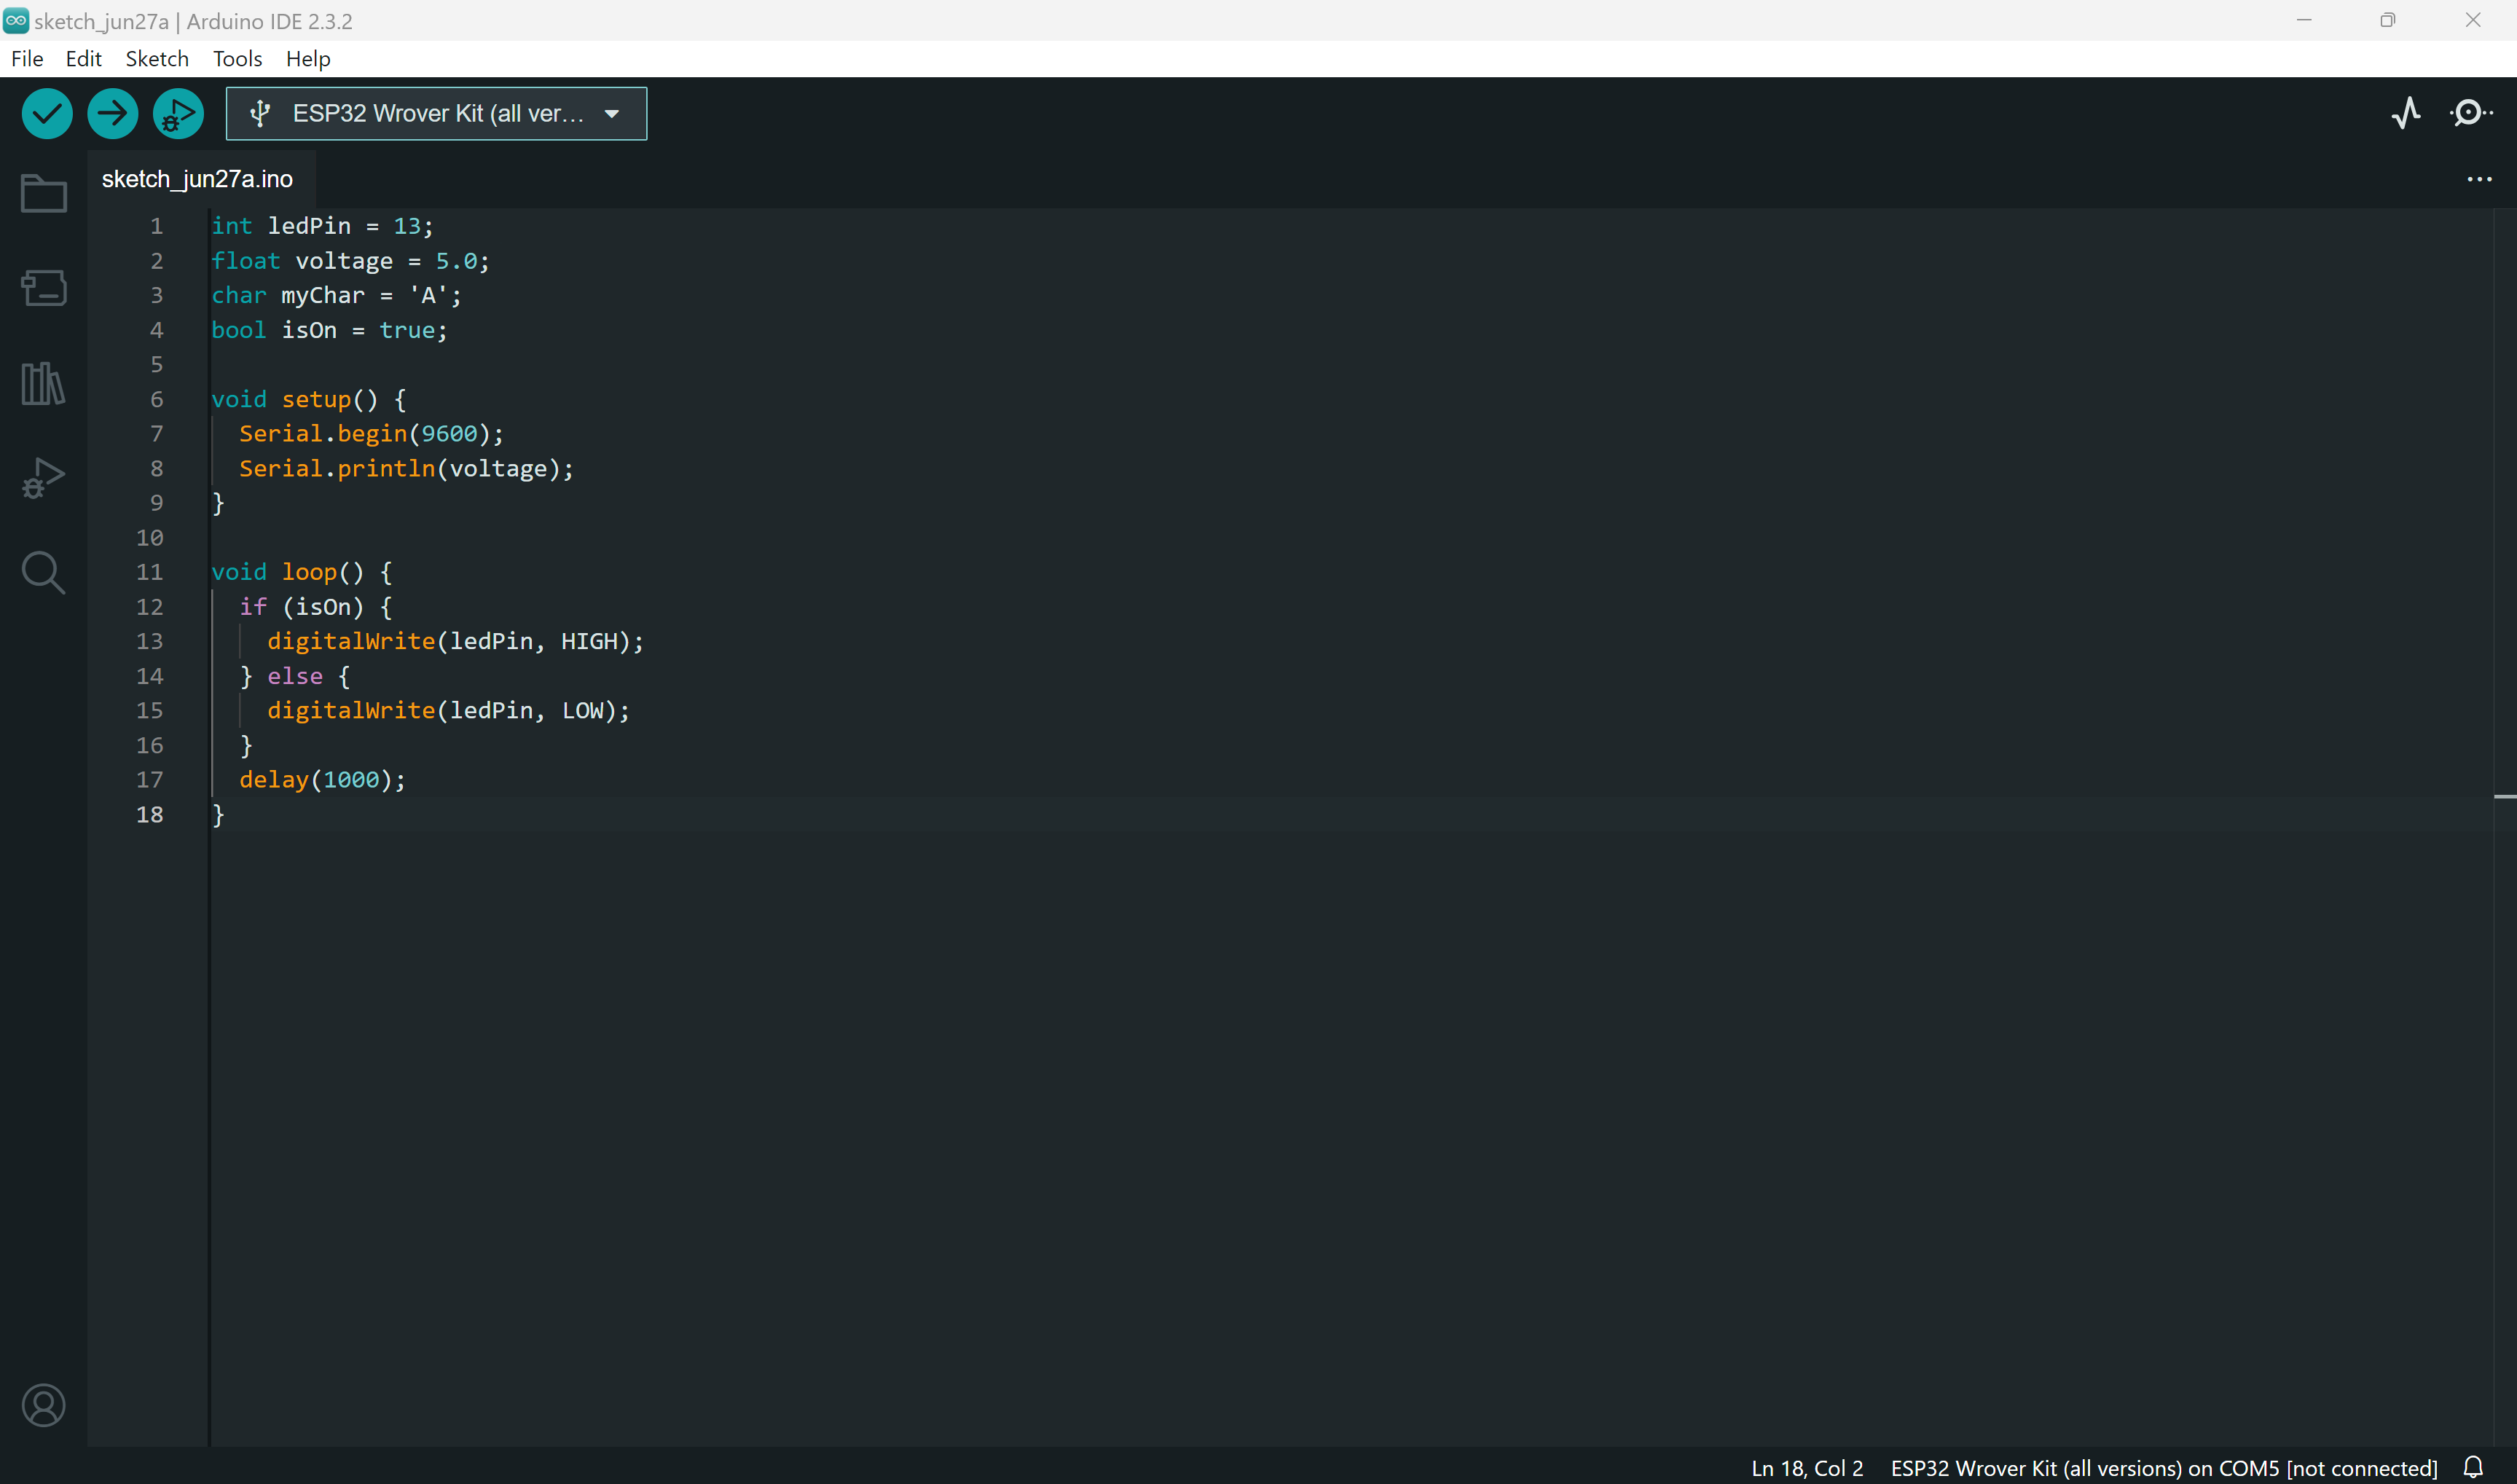
\includegraphics[width=\textwidth]{fig/fig5.png}
	\caption{C++ Data Types}
	\label{fig:5}
\end{figure}

\section{C++ Operators}
\textbf{Teori:} Operatorer bruges til at udføre operationer på variabler og værdier. Aritmetiske operatorer (\texttt{+}, \texttt{-}, \texttt{*}, \texttt{/}) bruges til matematiske operationer. Logiske operatorer (\texttt{\&\&}, \texttt{||}, \texttt{!}) bruges til at kombinere eller negere betingelser. Tildelingsoperatoren (\texttt{=}) bruges til at tildele værdier til variabler.
\newline\newline
\noindent\textbf{Eksempel:}
\begin{lstlisting}[language=C++]
	int a = 5;
	int b = 10;
	int sum = a + b;
	bool result = (a < b) && (b > 0);
	
	void setup() {
		Serial.begin(9600);
		Serial.println(sum);
		Serial.println(result);
	}
	
	void loop() {
		// empty loop
	}
\end{lstlisting}
\begin{figure}[h!]
	\centering
	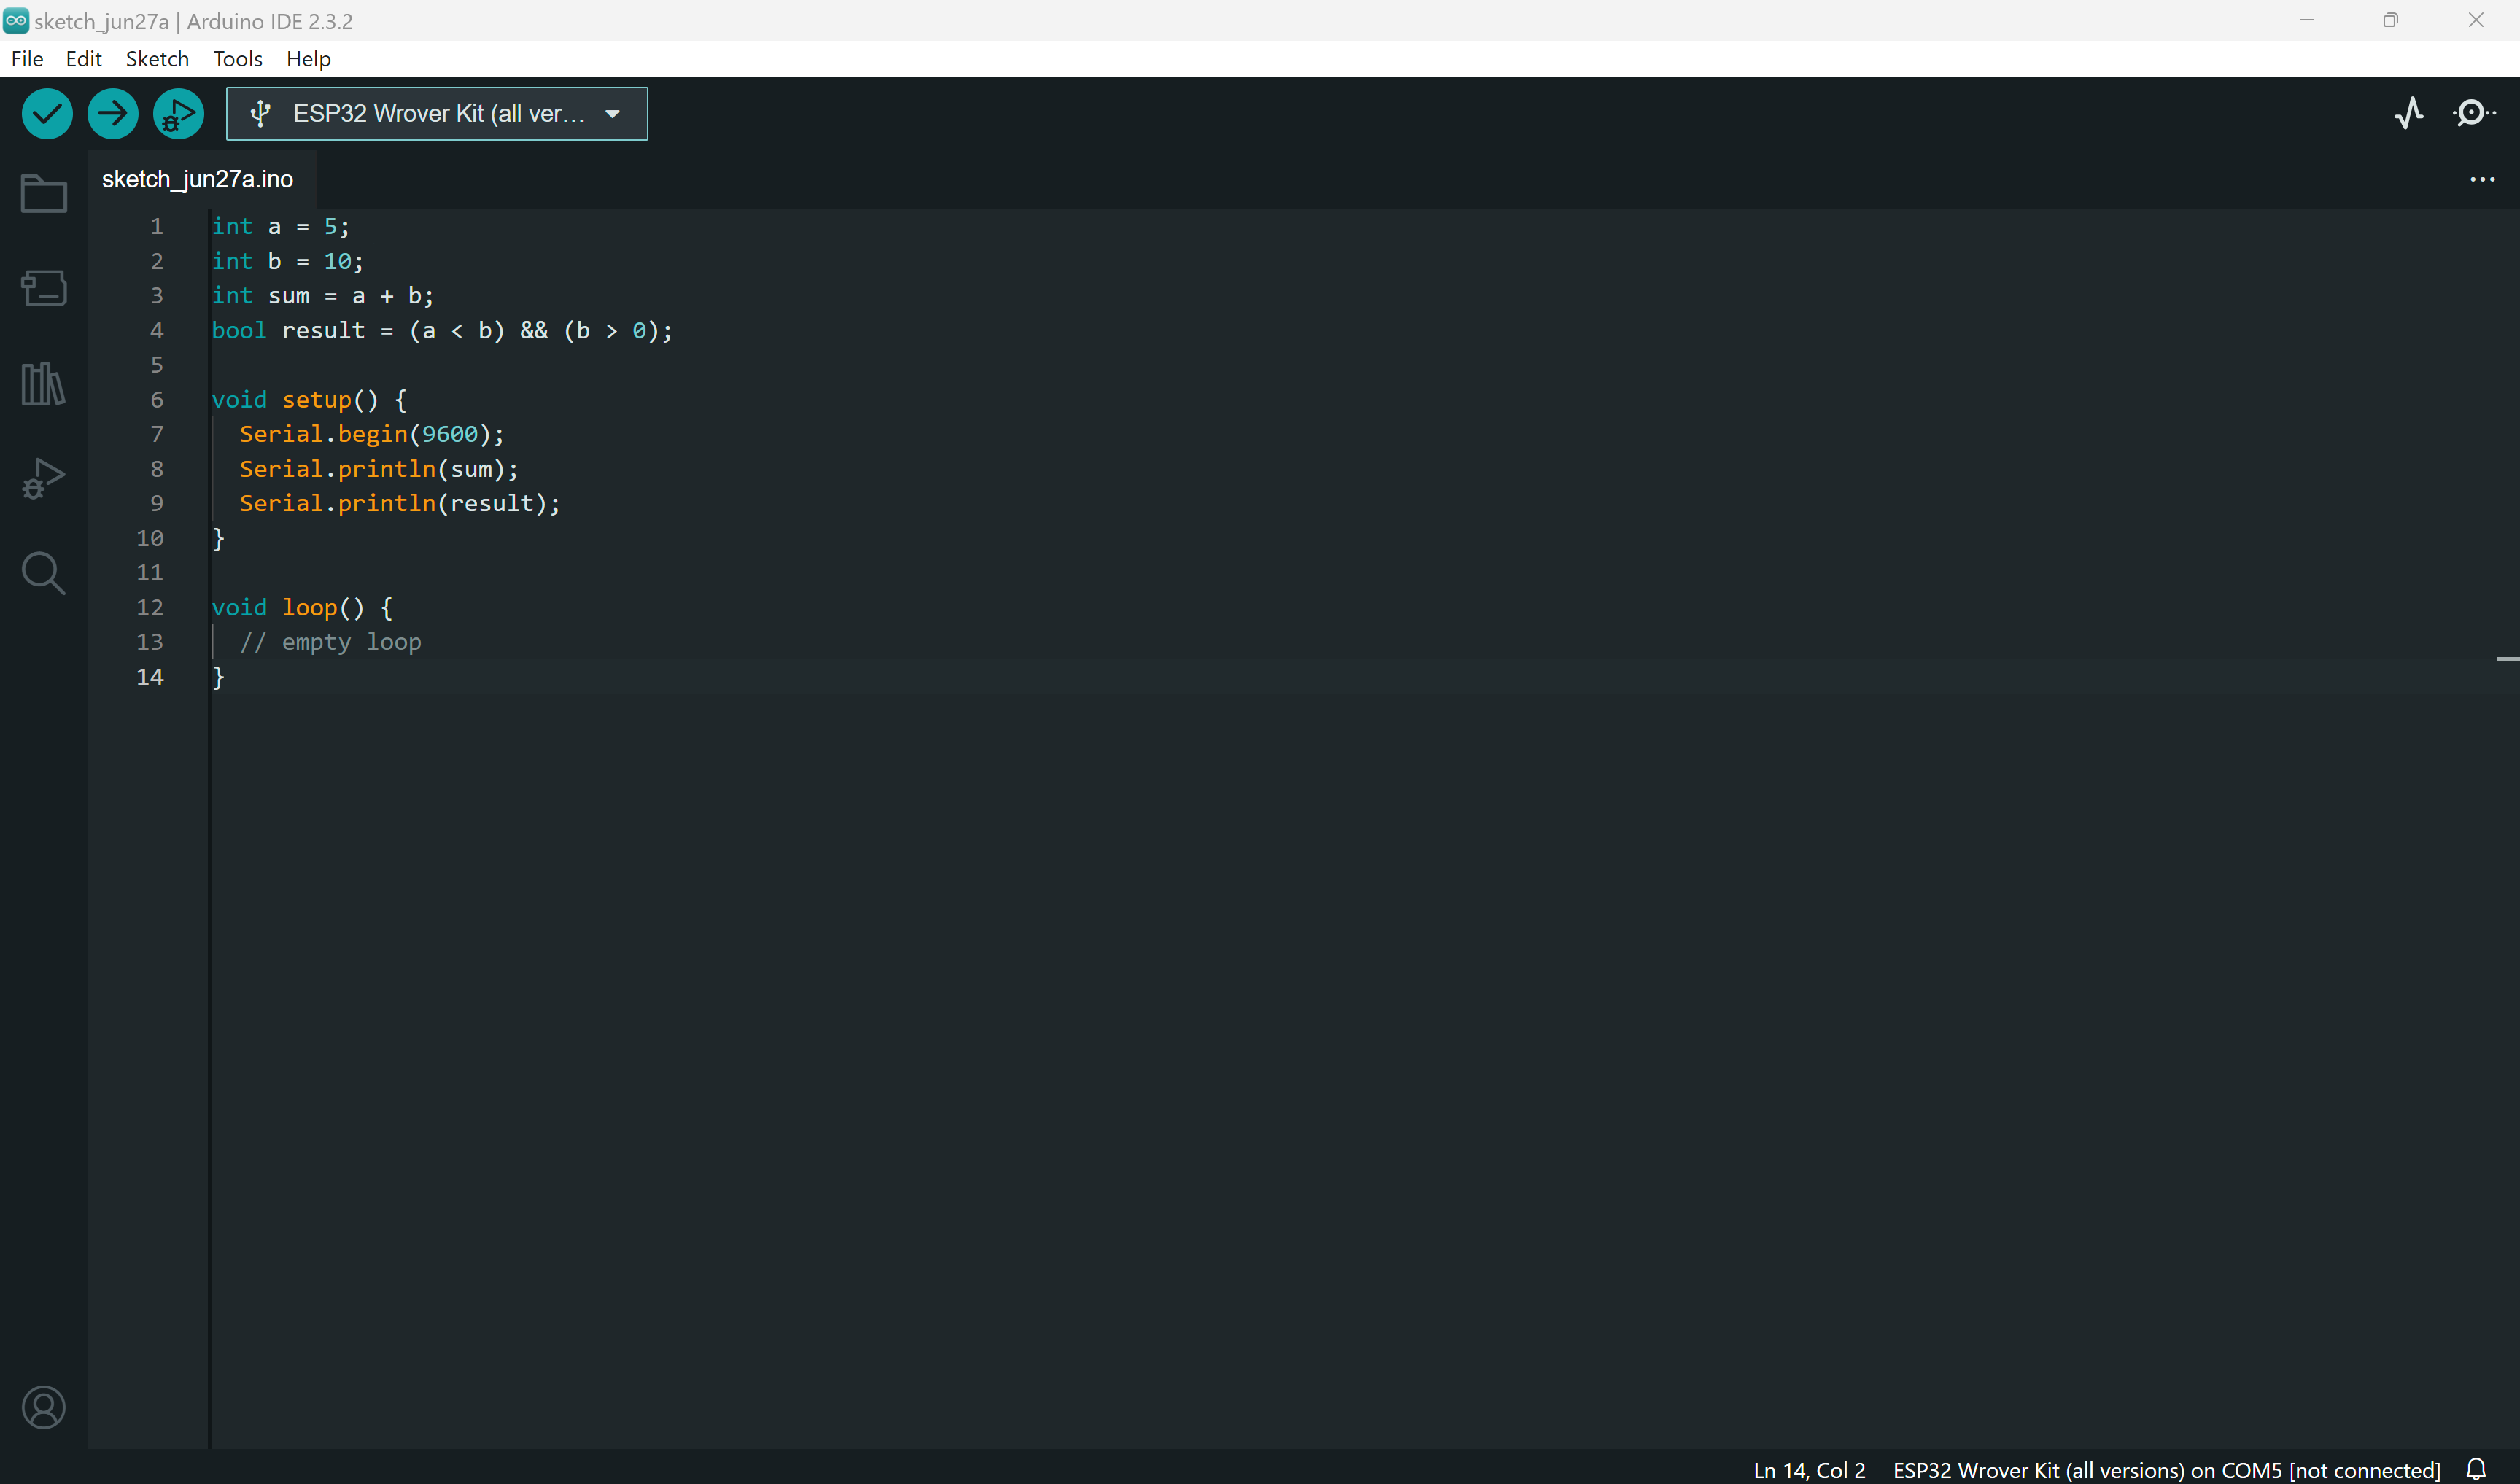
\includegraphics[width=\textwidth]{fig/fig6.png}
	\caption{C++ Operators}
	\label{fig:6}
\end{figure}

\section{C++ Strings}
\textbf{Teori:} Strings i C++ bruges til at holde tekst. De kan håndteres ved hjælp af String klassen i Arduino. Strings kan konkateneres, sammenlignes, og manipuleres på forskellige måder. Stringmanipulation er nyttig til at formatere og vise tekstbaseret data.
\newline\newline
\noindent\textbf{Eksempel:}
\begin{lstlisting}[language=C++]
	String greeting = "Hello";
	String name = "Arduino";
	String message = greeting + ", " + name + "!";
	
	void setup() {
		Serial.begin(9600);
		Serial.println(message);
	}
	
	void loop() {
		// empty loop
	}
\end{lstlisting}
\begin{figure}[h!]
	\centering
	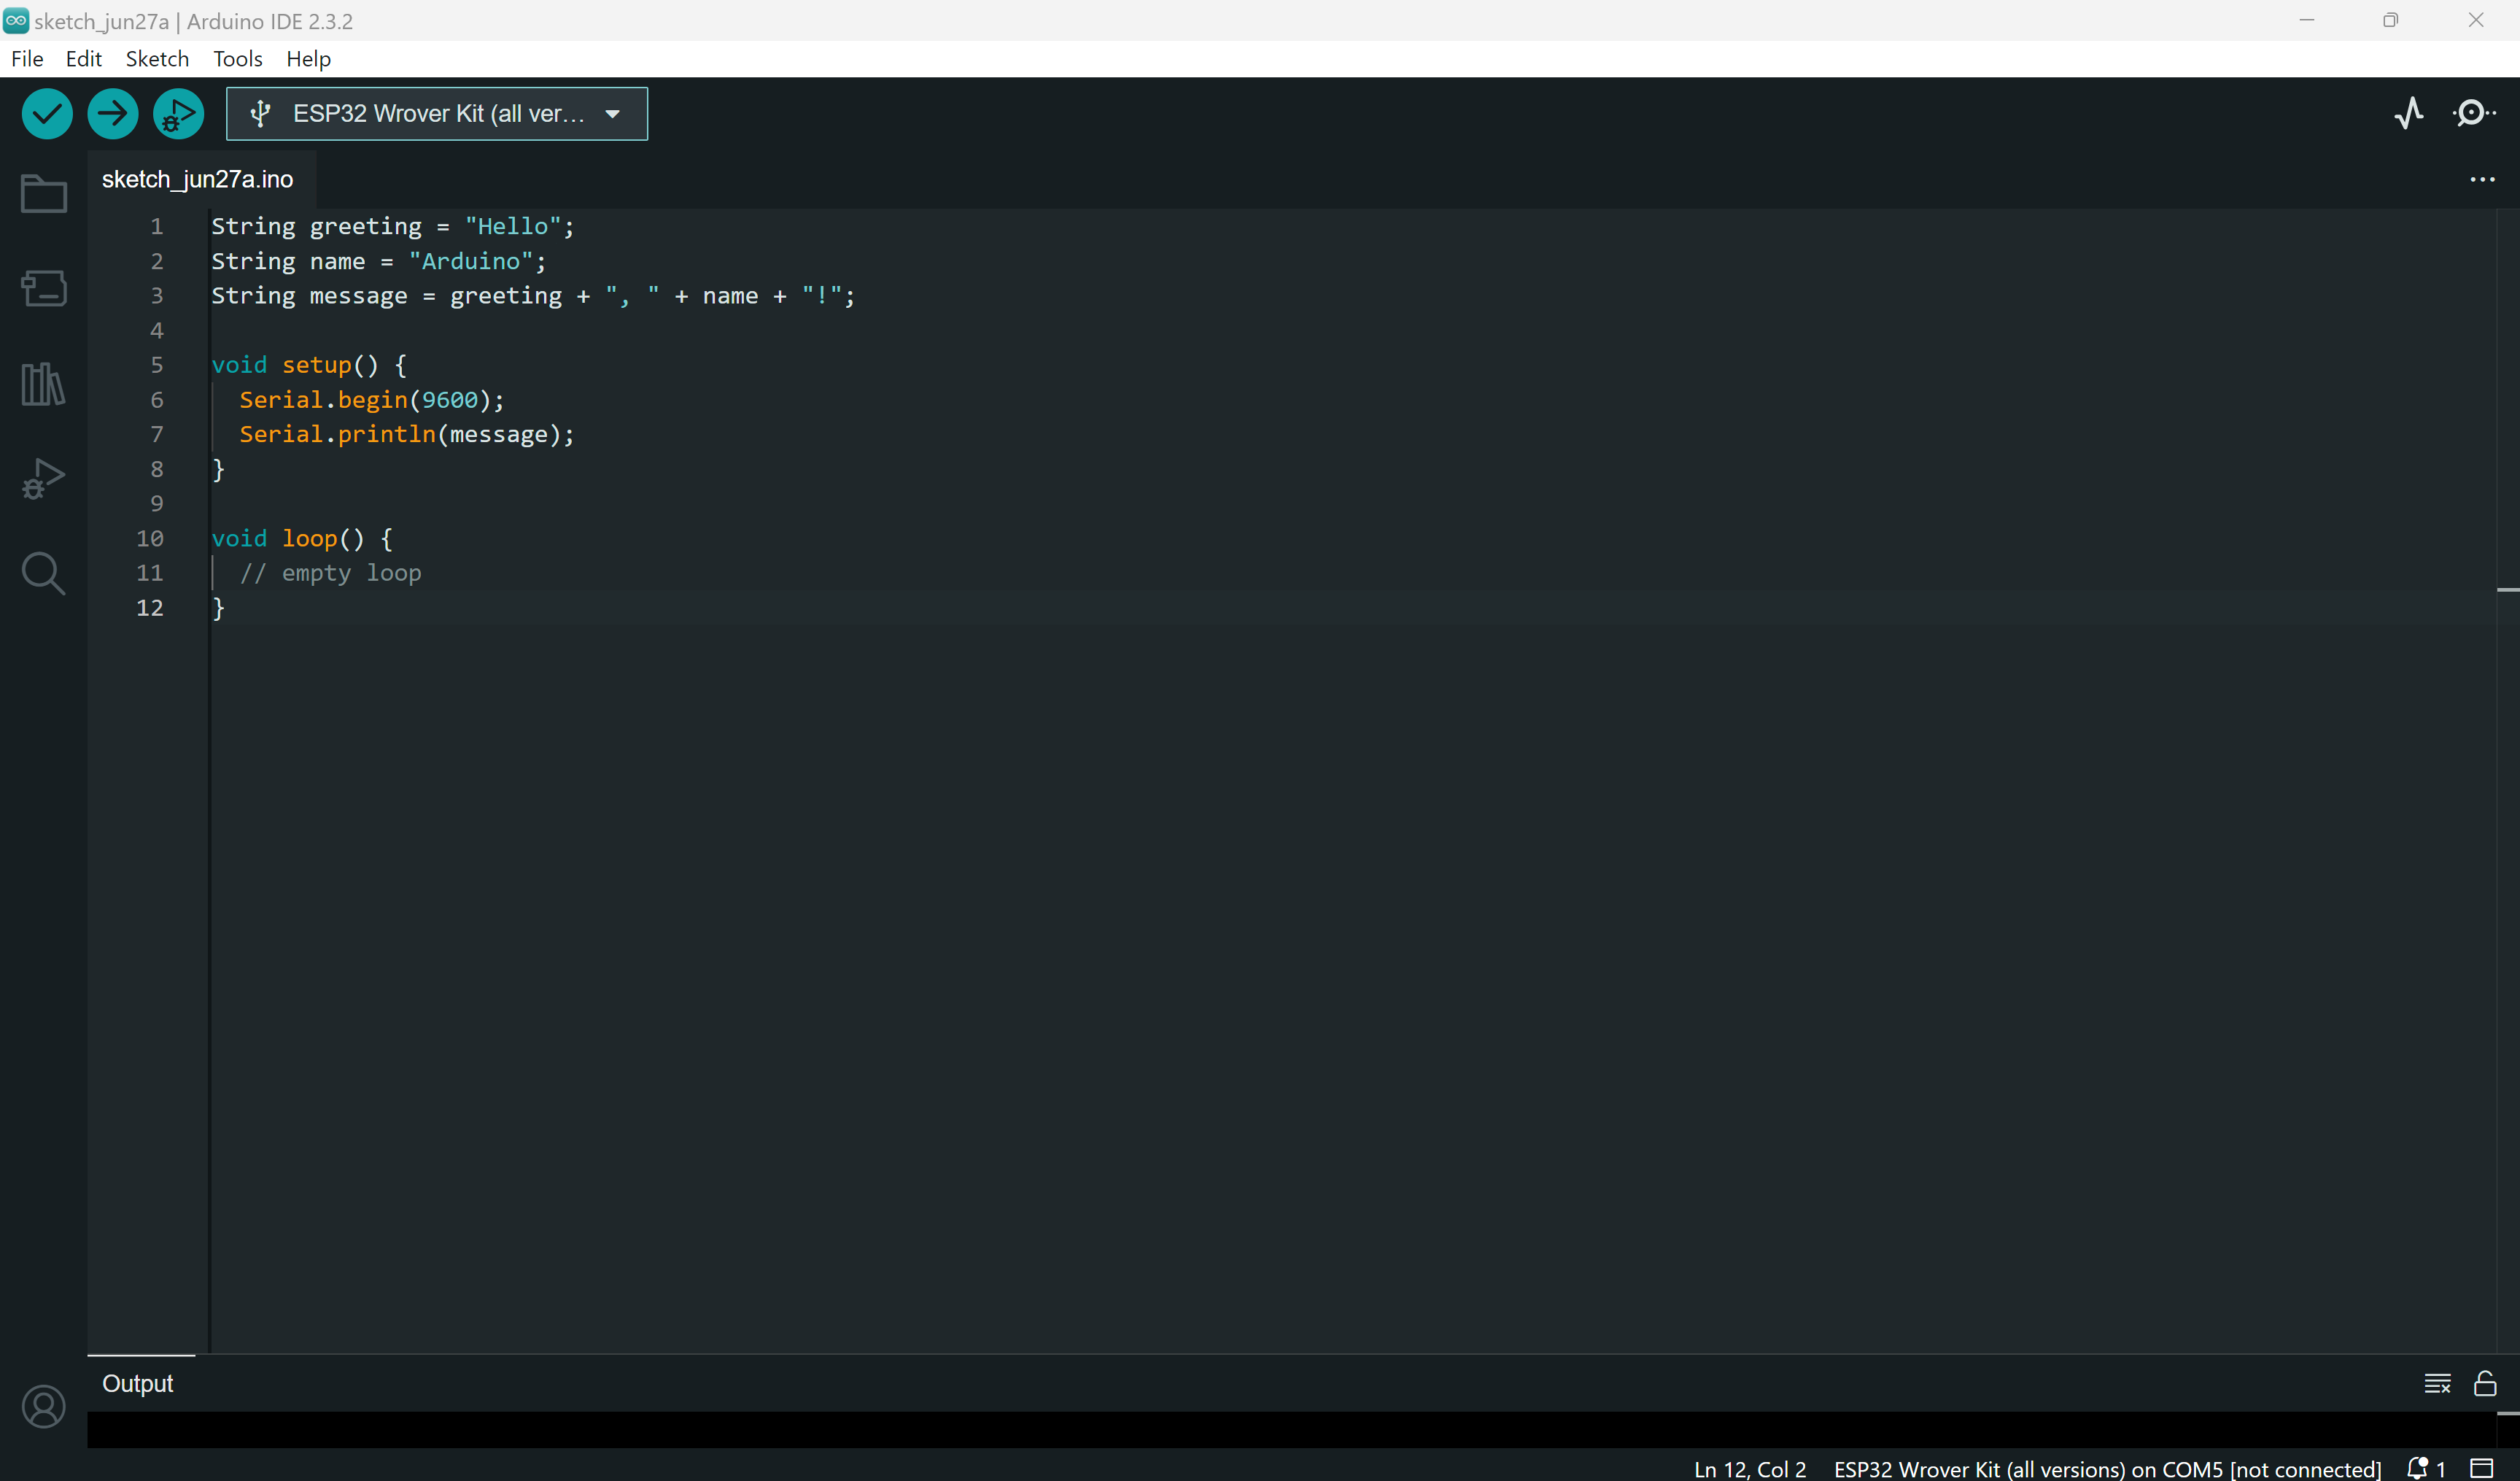
\includegraphics[width=\textwidth]{fig/fig7.png}
	\caption{C++ Strings}
	\label{fig:7}
\end{figure}

\section{C++ Conditions}
\textbf{Teori:} Betingede udsagn (if-else) bruges til at udføre forskellige handlinger baseret på forskellige betingelser. If-else strukturer tillader programmet at træffe beslutninger baseret på input eller tilstande. Komplekse beslutningstræer kan bygges ved at kombinere flere if-else udsagn. En anden betinget udsagn \texttt{case}.
\newline\newline
\noindent\textbf{Eksempel: \texttt{if}}
\begin{lstlisting}[language=C++]
	int sensorValue = 0;
	
	void setup() {
		Serial.begin(9600);
	}
	
	void loop() {
		sensorValue = analogRead(A0);
		if (sensorValue > 500) {
			Serial.println("High");
		} else {
			Serial.println("Low");
		}
		delay(1000);}
\end{lstlisting}
\begin{figure}[h!]
	\centering
	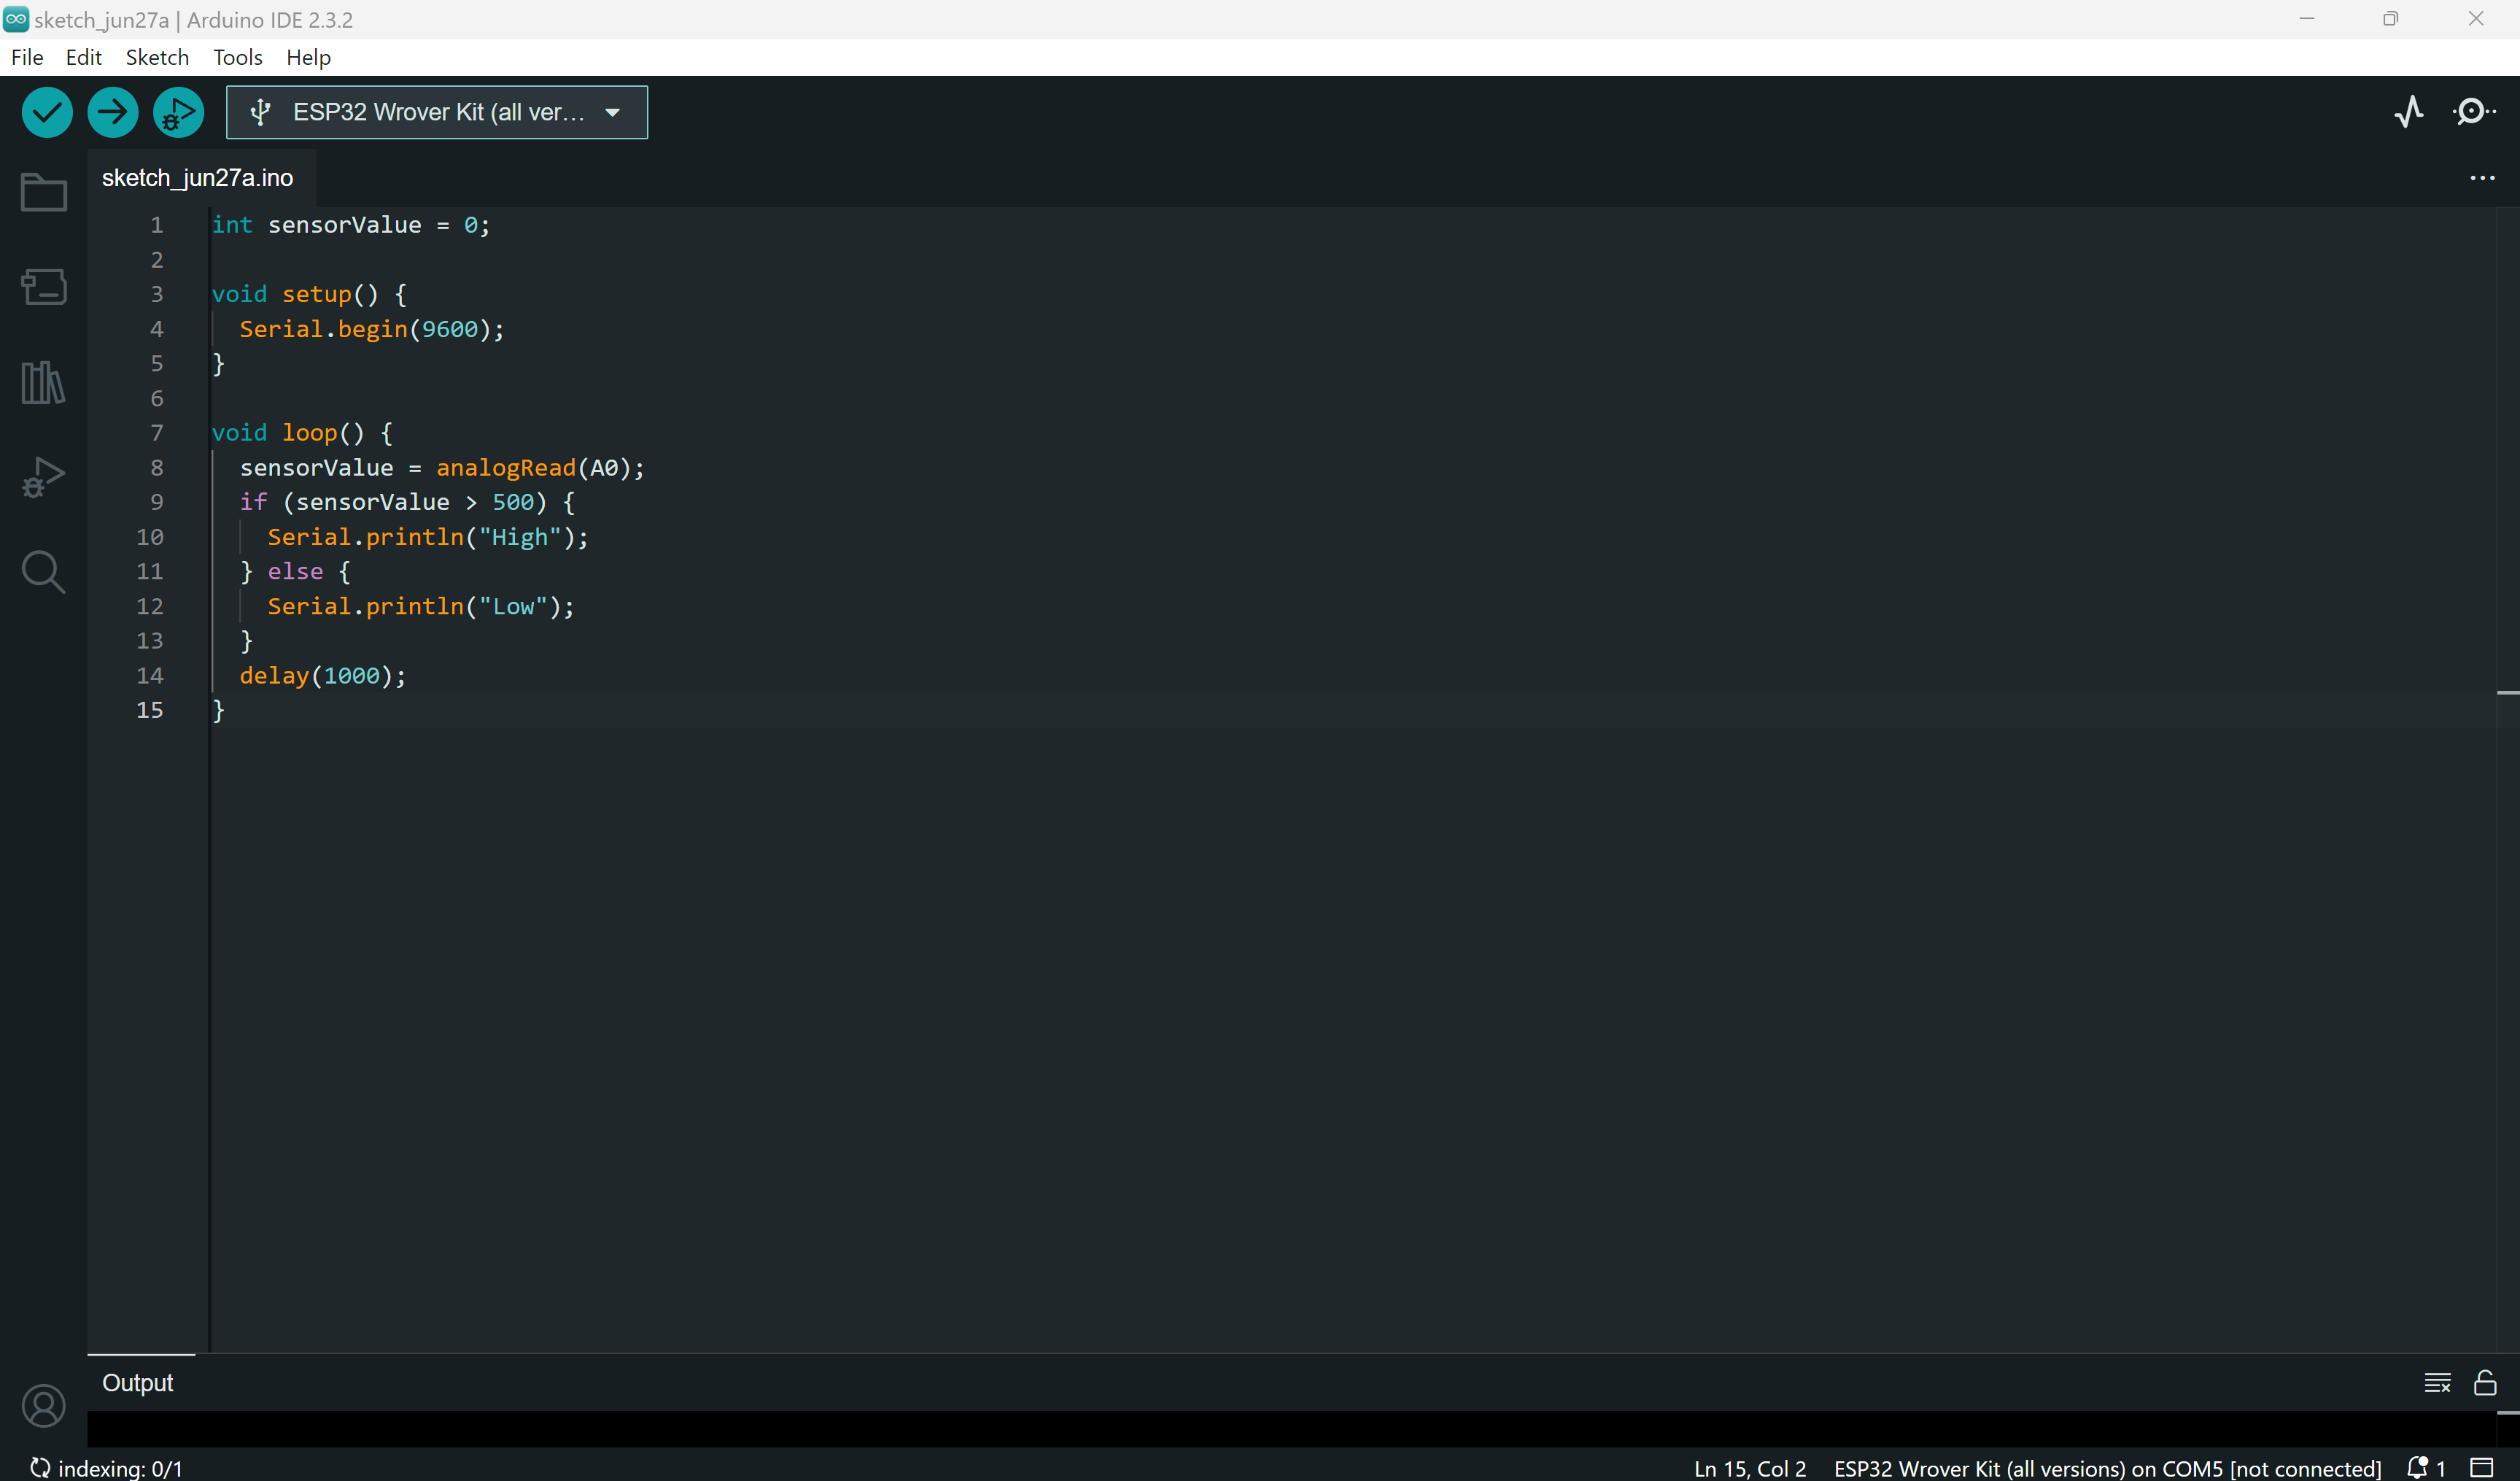
\includegraphics[width=\textwidth]{fig/fig8.png}
	\caption{C++ Conditions}
	\label{fig:8}
\end{figure}
\clearpage
\noindent\textbf{Eksempel: \texttt{case}}
\begin{lstlisting}[language=C++]
	int ledPin = 13;
	int command = 1;
	int button = 8;
	
	// Initialize with LOW because of pull-down resistor
	int lastButtonState = LOW;
	
	// Current reading from the input pin 
	int buttonState; 
	
	// the last time the output pin was toggled
	unsigned long lastDebounceTime = 0;
	
	// the debounce time; increase if the output flickers 
	unsigned long debounceDelay = 50; 
	
	void setup() {
		pinMode(ledPin, OUTPUT);
		pinMode(button, INPUT); 
		Serial.begin(9600);
		
		// Ensure LED is off initially
		digitalWrite(ledPin, LOW); 
	}
	
	void loop() {
		// Read the state of the switch into a local variable:
		int reading = digitalRead(button);
		
		// Check to see if you just pressed the button
		// (i.e. the input went from LOW to HIGH), and you've 
		//waited long enough
		// since the last press to ignore any noise:
		if (reading != lastButtonState) {
			// reset the debouncing timer
			lastDebounceTime = millis();
		}
		Serial.println(reading);
		if ((millis() - lastDebounceTime) > debounceDelay) {
			// whatever the reading is at, it's been there for 
			// longer than the debounce
			// delay, so take it as the actual current state:
			
			// if the button state has changed:
			if (reading != buttonState) {
				buttonState = reading;
				
				// only toggle the LED if the new button state is 
				//HIGH
				if (buttonState == HIGH) {
					switch (command) {
						case 1:
						Serial.println(buttonState);
						command = 0;
						break;
						case 0:
						Serial.println(buttonState);
						command = 1;
						break;
						default:
						// Do nothing
						break;
					}
				}
			}
		}
		
		// Save the reading. Next time through the loop, 
		// it'll be the lastButtonState:
		lastButtonState = reading;
		
		// Actions
		switch (command) {
			case 1:
			digitalWrite(ledPin, HIGH); // Turn LED on
			break;
			case 0:
			digitalWrite(ledPin, LOW); // Turn LED off
			break;
			default:
			// Do nothing
			break;
		}
	}
\end{lstlisting}
\clearpage
\section{C++ Loops}
\textbf{Teori:} Loops bruges til at udføre en blok kode gentagne gange. De mest almindelige loops er \texttt{while} og \texttt{for} loops. While loop udfører kodeblokken så længe betingelsen er sand, mens for loop bruges til at gentage en blok kode et bestemt antal gange. Loops er essentielle for gentagne opgaver som sensorlæsninger og LED blinkning.

\subsubsection{C++ While Loop}
\textbf{Teori:} \texttt{while} loop kontrollerer en betingelse og udfører kodeblokken gentagne gange så længe betingelsen er sand. Dette er nyttigt til opgaver, der skal fortsætte, indtil en bestemt tilstand ændres.
\newline\newline
\noindent\textbf{Eksempel:}
\begin{lstlisting}[language=C++]
	int i = 0;
	
	void setup() {
		Serial.begin(9600);
	}
	
	void loop() {
		while (i < 5) {
			Serial.println(i);
			i++;
		}
		delay(1000); // wait for a second before running again
	}
\end{lstlisting}
\begin{figure}[h!]
	\centering
	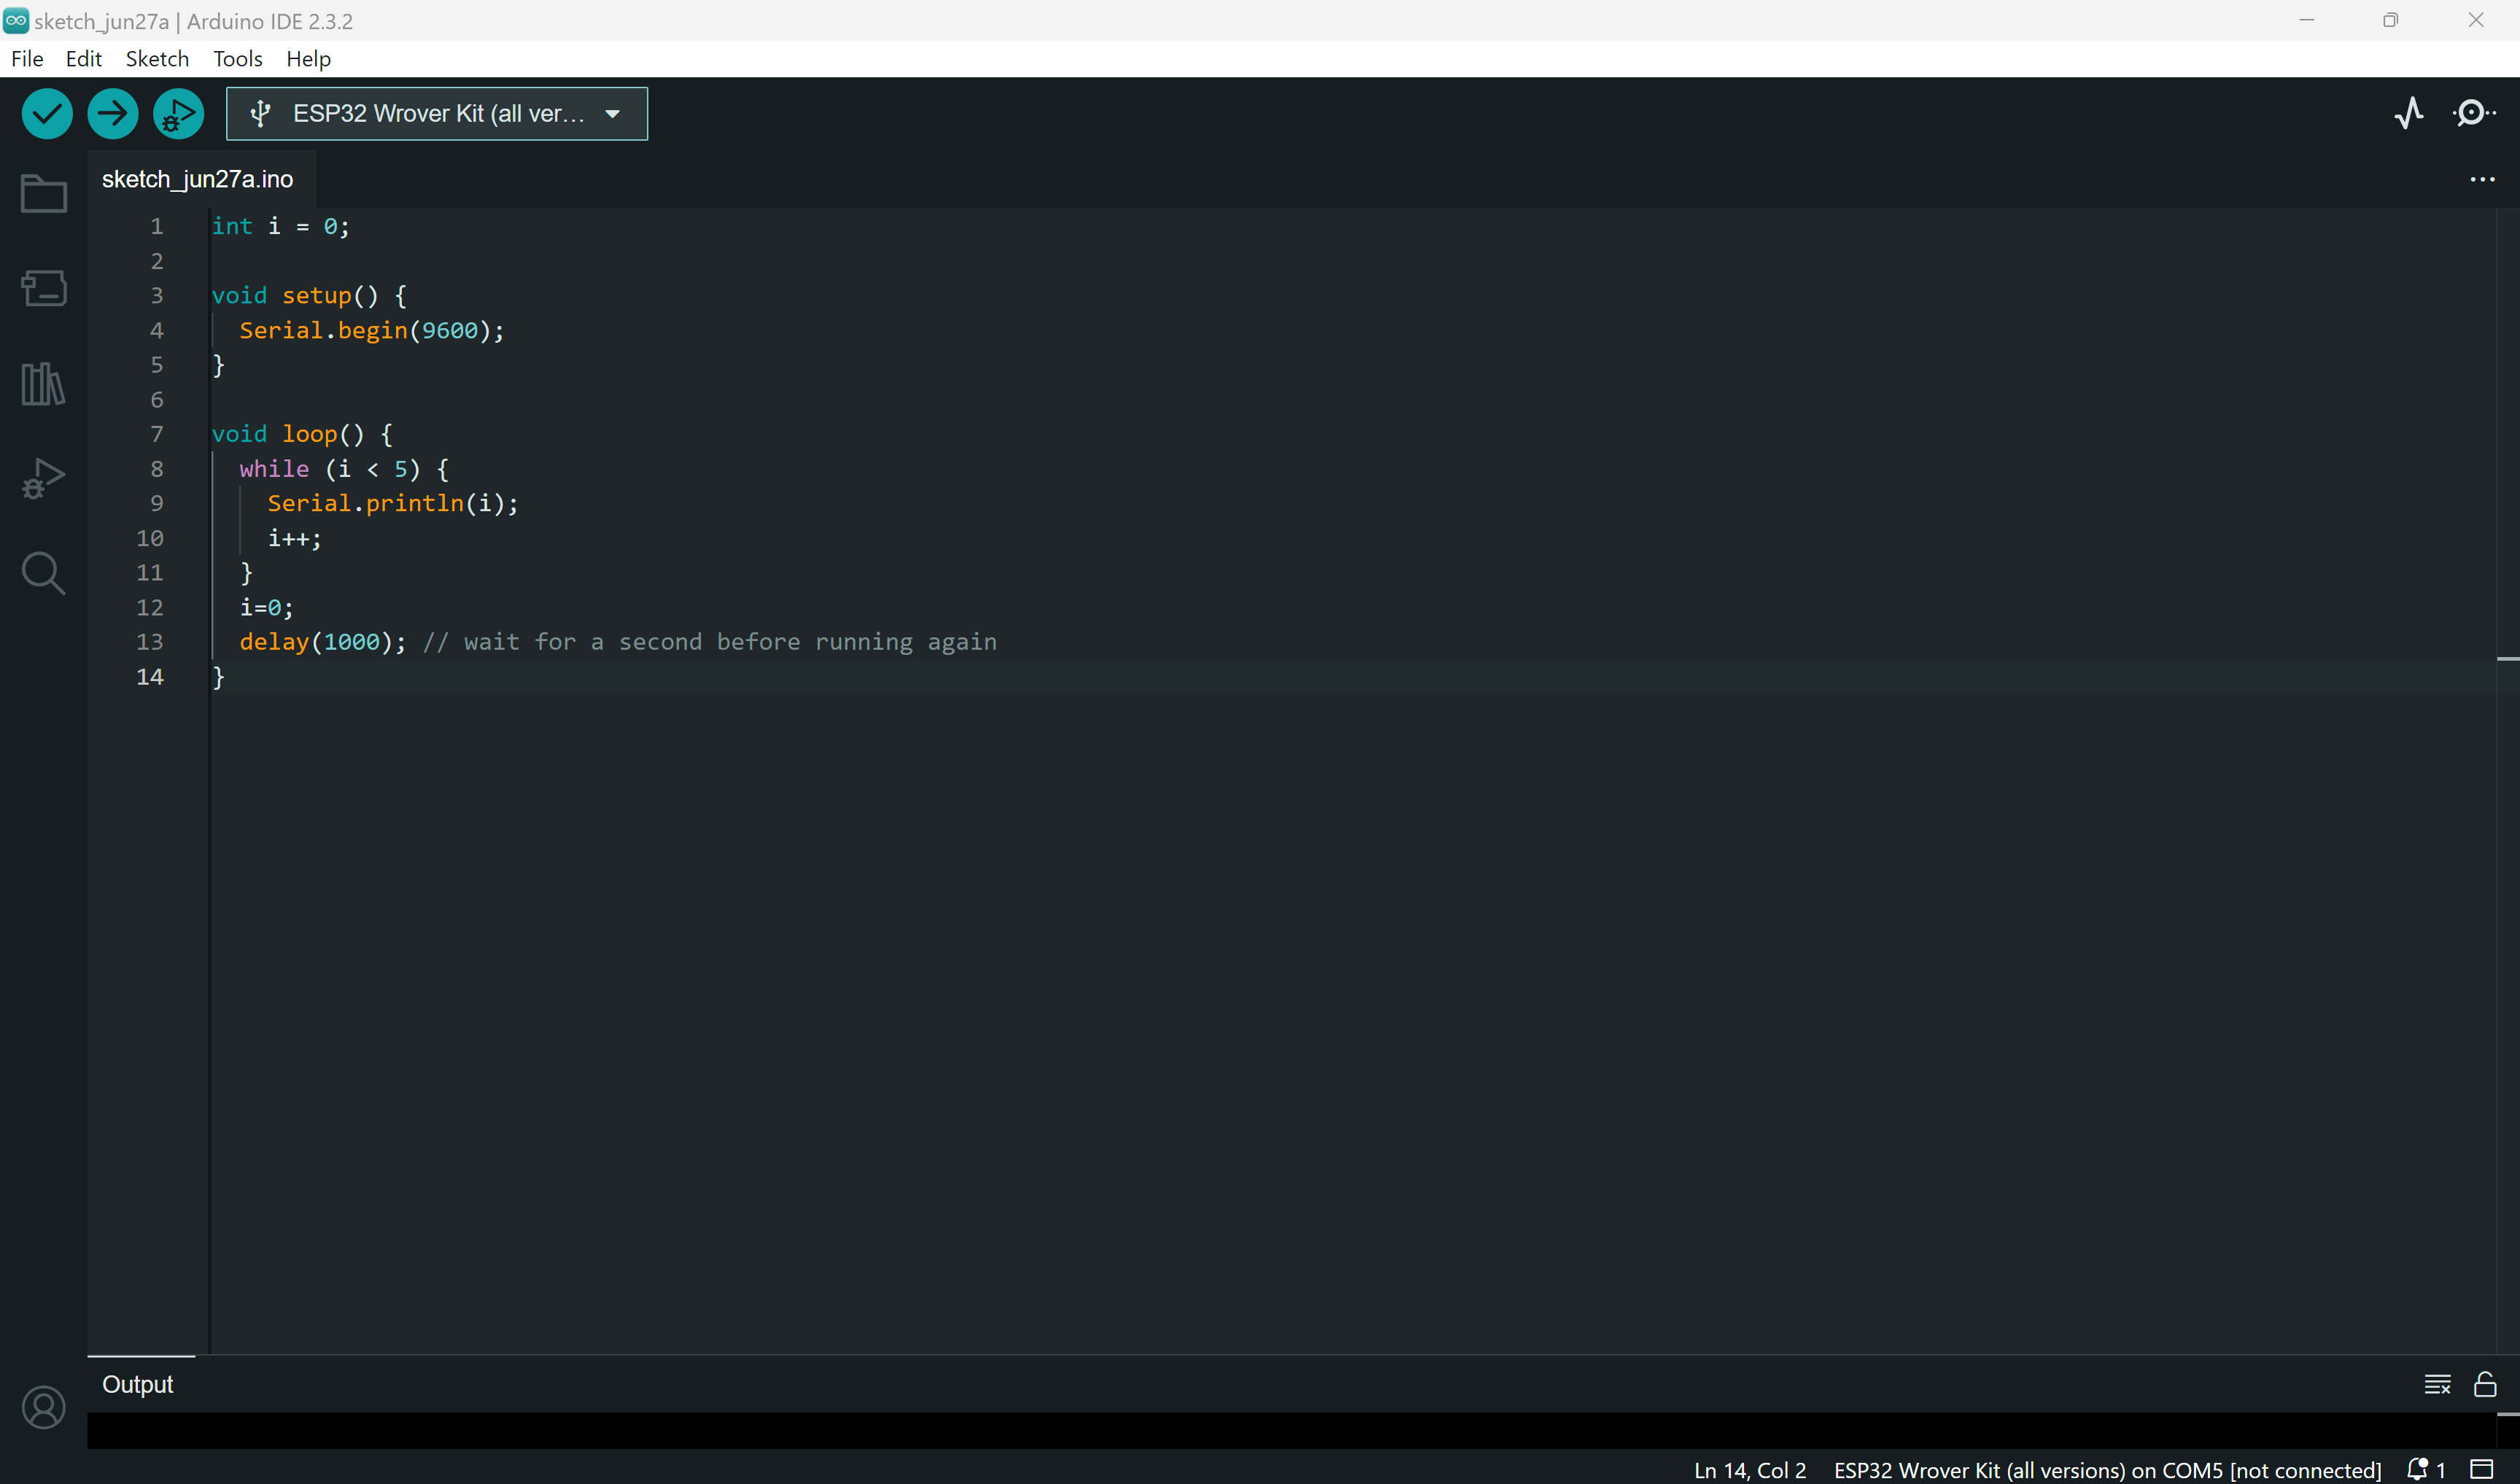
\includegraphics[width=\textwidth]{fig/fig9.png}
	\caption{while}
	\label{fig:9}
\end{figure}

\subsubsection{C++ For Loop}
\textbf{Teori:} \texttt{for} loop initialiserer en variabel, kontrollerer en betingelse og opdaterer variablen i hver iteration. For loops bruges ofte, når antallet af iterationer er kendt på forhånd.
\newline\newline
\noindent\textbf{Eksempel:}
\begin{lstlisting}[language=C++]
	void setup() {
		Serial.begin(9600);
	}
	
	void loop() {
		for (int i = 0; i < 5; i++) {
			Serial.println(i);
		}
		delay(1000); // wait for a second before running again
	}
\end{lstlisting}
\begin{figure}[h!]
	\centering
	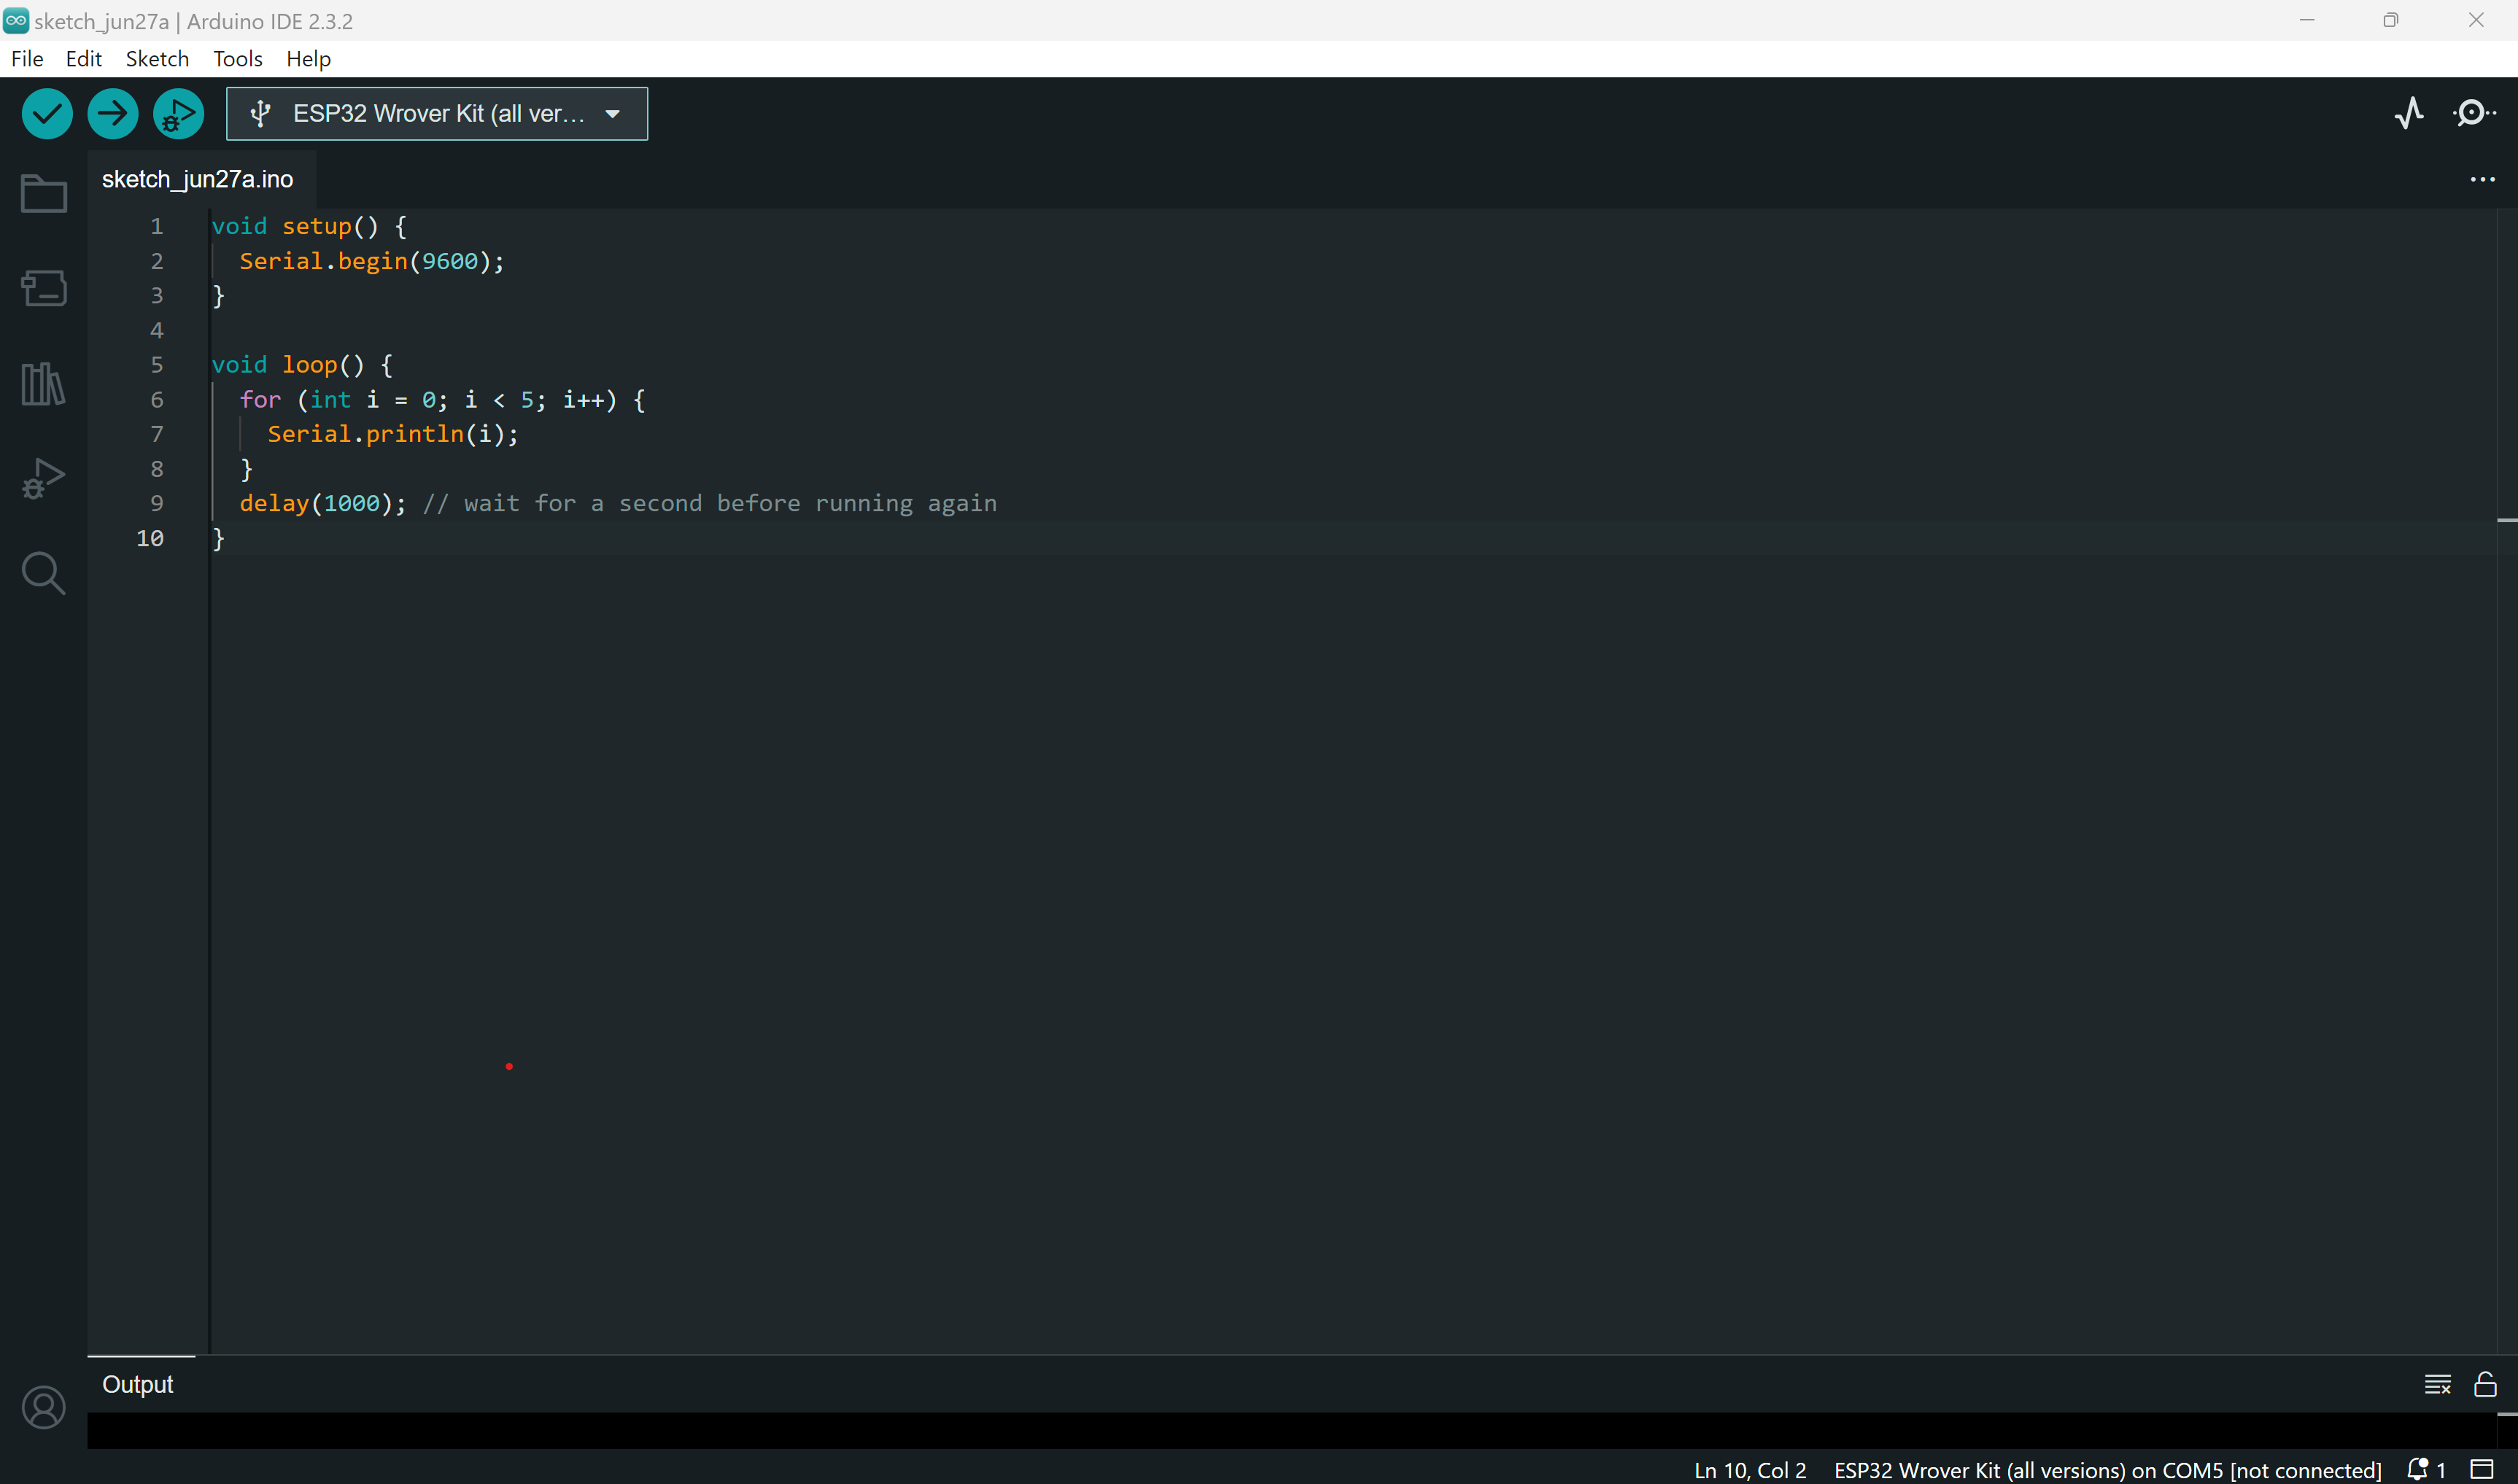
\includegraphics[width=\textwidth]{fig/fig10.png}
	\caption{For Loop}
	\label{fig:10}
\end{figure}

\section{C++ Functions}
\textbf{Formål:} Dette afsnit dækker funktioner i C++, herunder parameteroverførsel, overloading, scope og rekursion. Studerende vil lære at skrive og bruge funktioner til at strukturere og organisere deres kode på Arduino. Funktioner gør koden mere modulær og genanvendelig.

\textbf{Læringsmål:} Efter at have læst dette afsnit forventes det, at studerende kan:
\begin{itemize}
	\item Skrive og kalde funktioner i Arduino-kode.
	\item Forstå og anvende funktionsparametre i Arduino.
	\item Implementere funktion overloading hvor det er relevant.
	\item Forstå begrebet scope og livstid af variabler i Arduino-kode.
	\item Anvende rekursion i løsningen af problemer på Arduino.
\end{itemize}

\subsection{C++ Functions}
\textbf{Teori:} Funktioner er blokke af kode, der udfører en specifik opgave og kan genbruges flere steder i programmet. Funktioner kan tage parametre og returnere værdier. Dette gør det muligt at sende data til og modtage data fra funktioner.
\newline\newline
\noindent\textbf{Eksempel:}
\begin{lstlisting}[language=C++]
	void blink(int times) {
		for (int i = 0; i < times; i++) {
			digitalWrite(13, HIGH);
			delay(500);
			digitalWrite(13, LOW);
			delay(500);
		}
	}
	
	void setup() {
		pinMode(13, OUTPUT);
	}
	
	void loop() {
		blink(3); // call the blink function with parameter 3
		delay(1000); // wait for a second before running again
	}
\end{lstlisting}
\begin{figure}[h!]
	\centering
	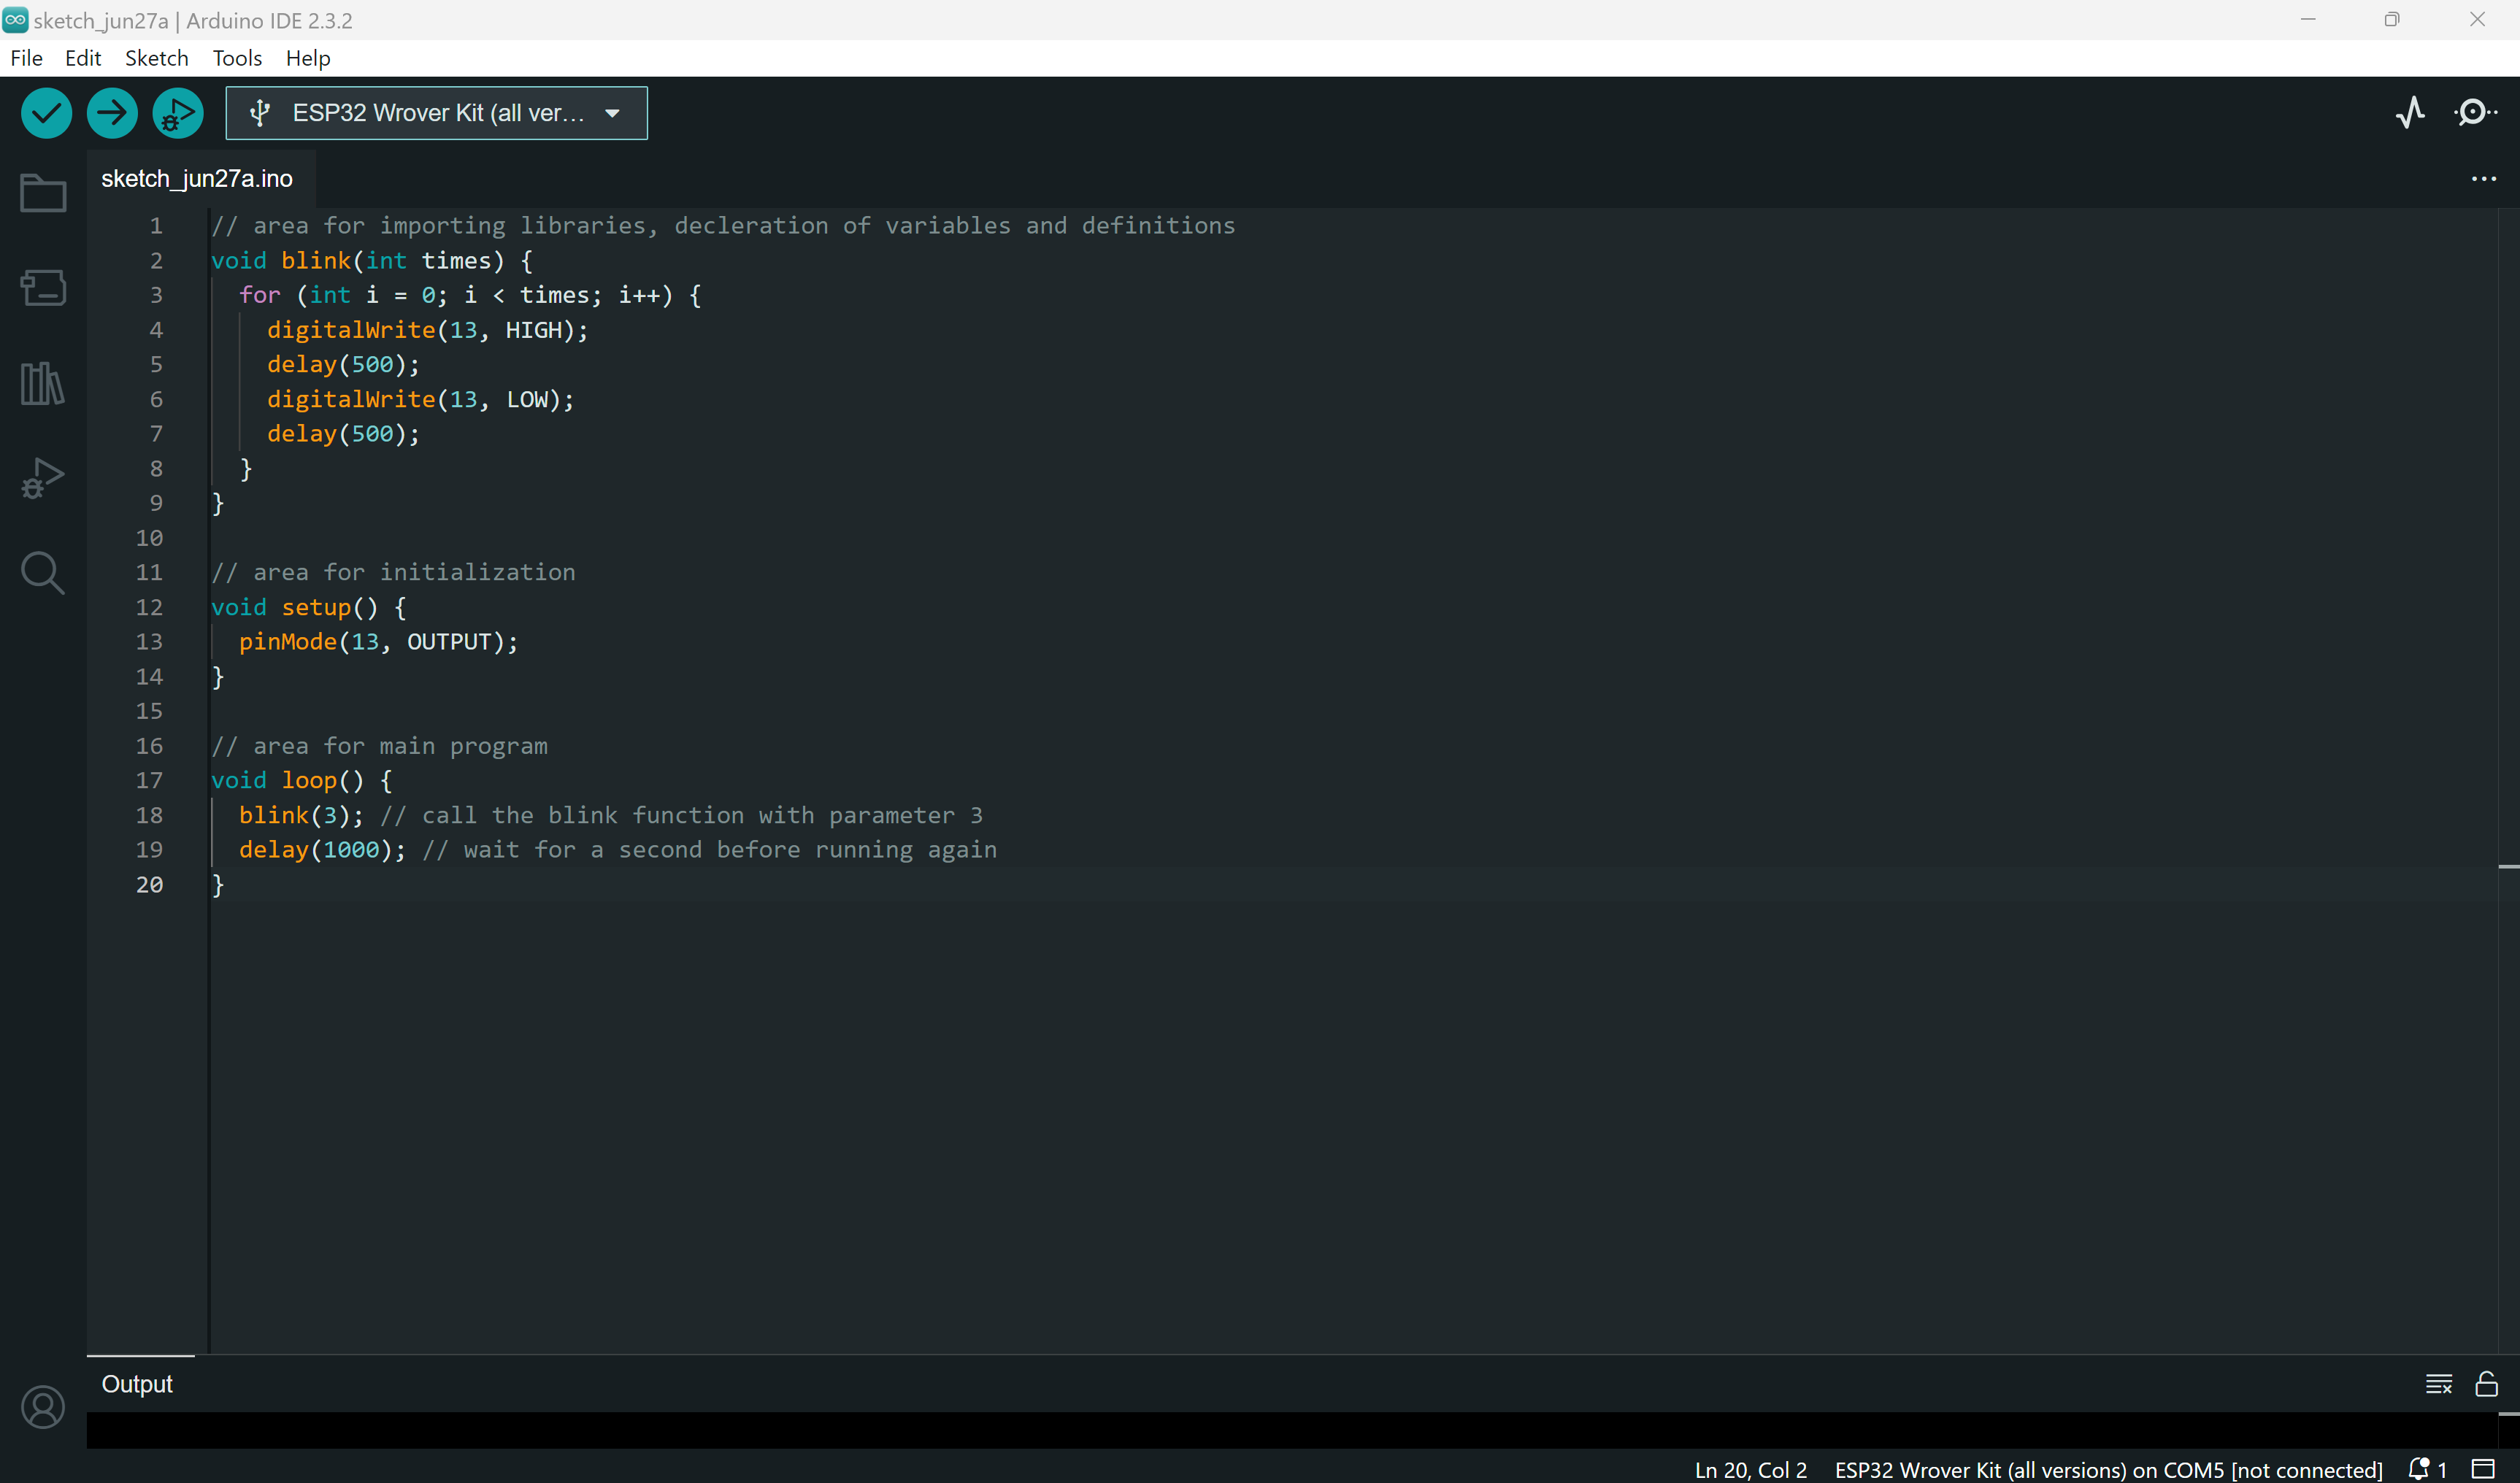
\includegraphics[width=\textwidth]{fig/fig11.png}
	\caption{text}
	\label{fig:11}
\end{figure}

\subsection{C++ Function Parameters}
\textbf{Teori:} Funktioner kan modtage input via parametre, som kan bruges inden i funktionen. Parametre specificeres i funktionsdeklarationen og defineres, når funktionen kaldes. Dette gør det muligt at skrive mere fleksible og genanvendelige funktioner.
\newline\newline
\noindent\textbf{Eksempel:}
\begin{lstlisting}[language=C++]
	void setup() {
		Serial.begin(9600);
	}
	
	void printMessage(String message) {
		Serial.println(message);
	}
	
	void loop() {
		printMessage("Hello, Arduino!"); // pass a string to the function
		delay(1000);
	}
\end{lstlisting}
\begin{figure}[h!]
	\centering
	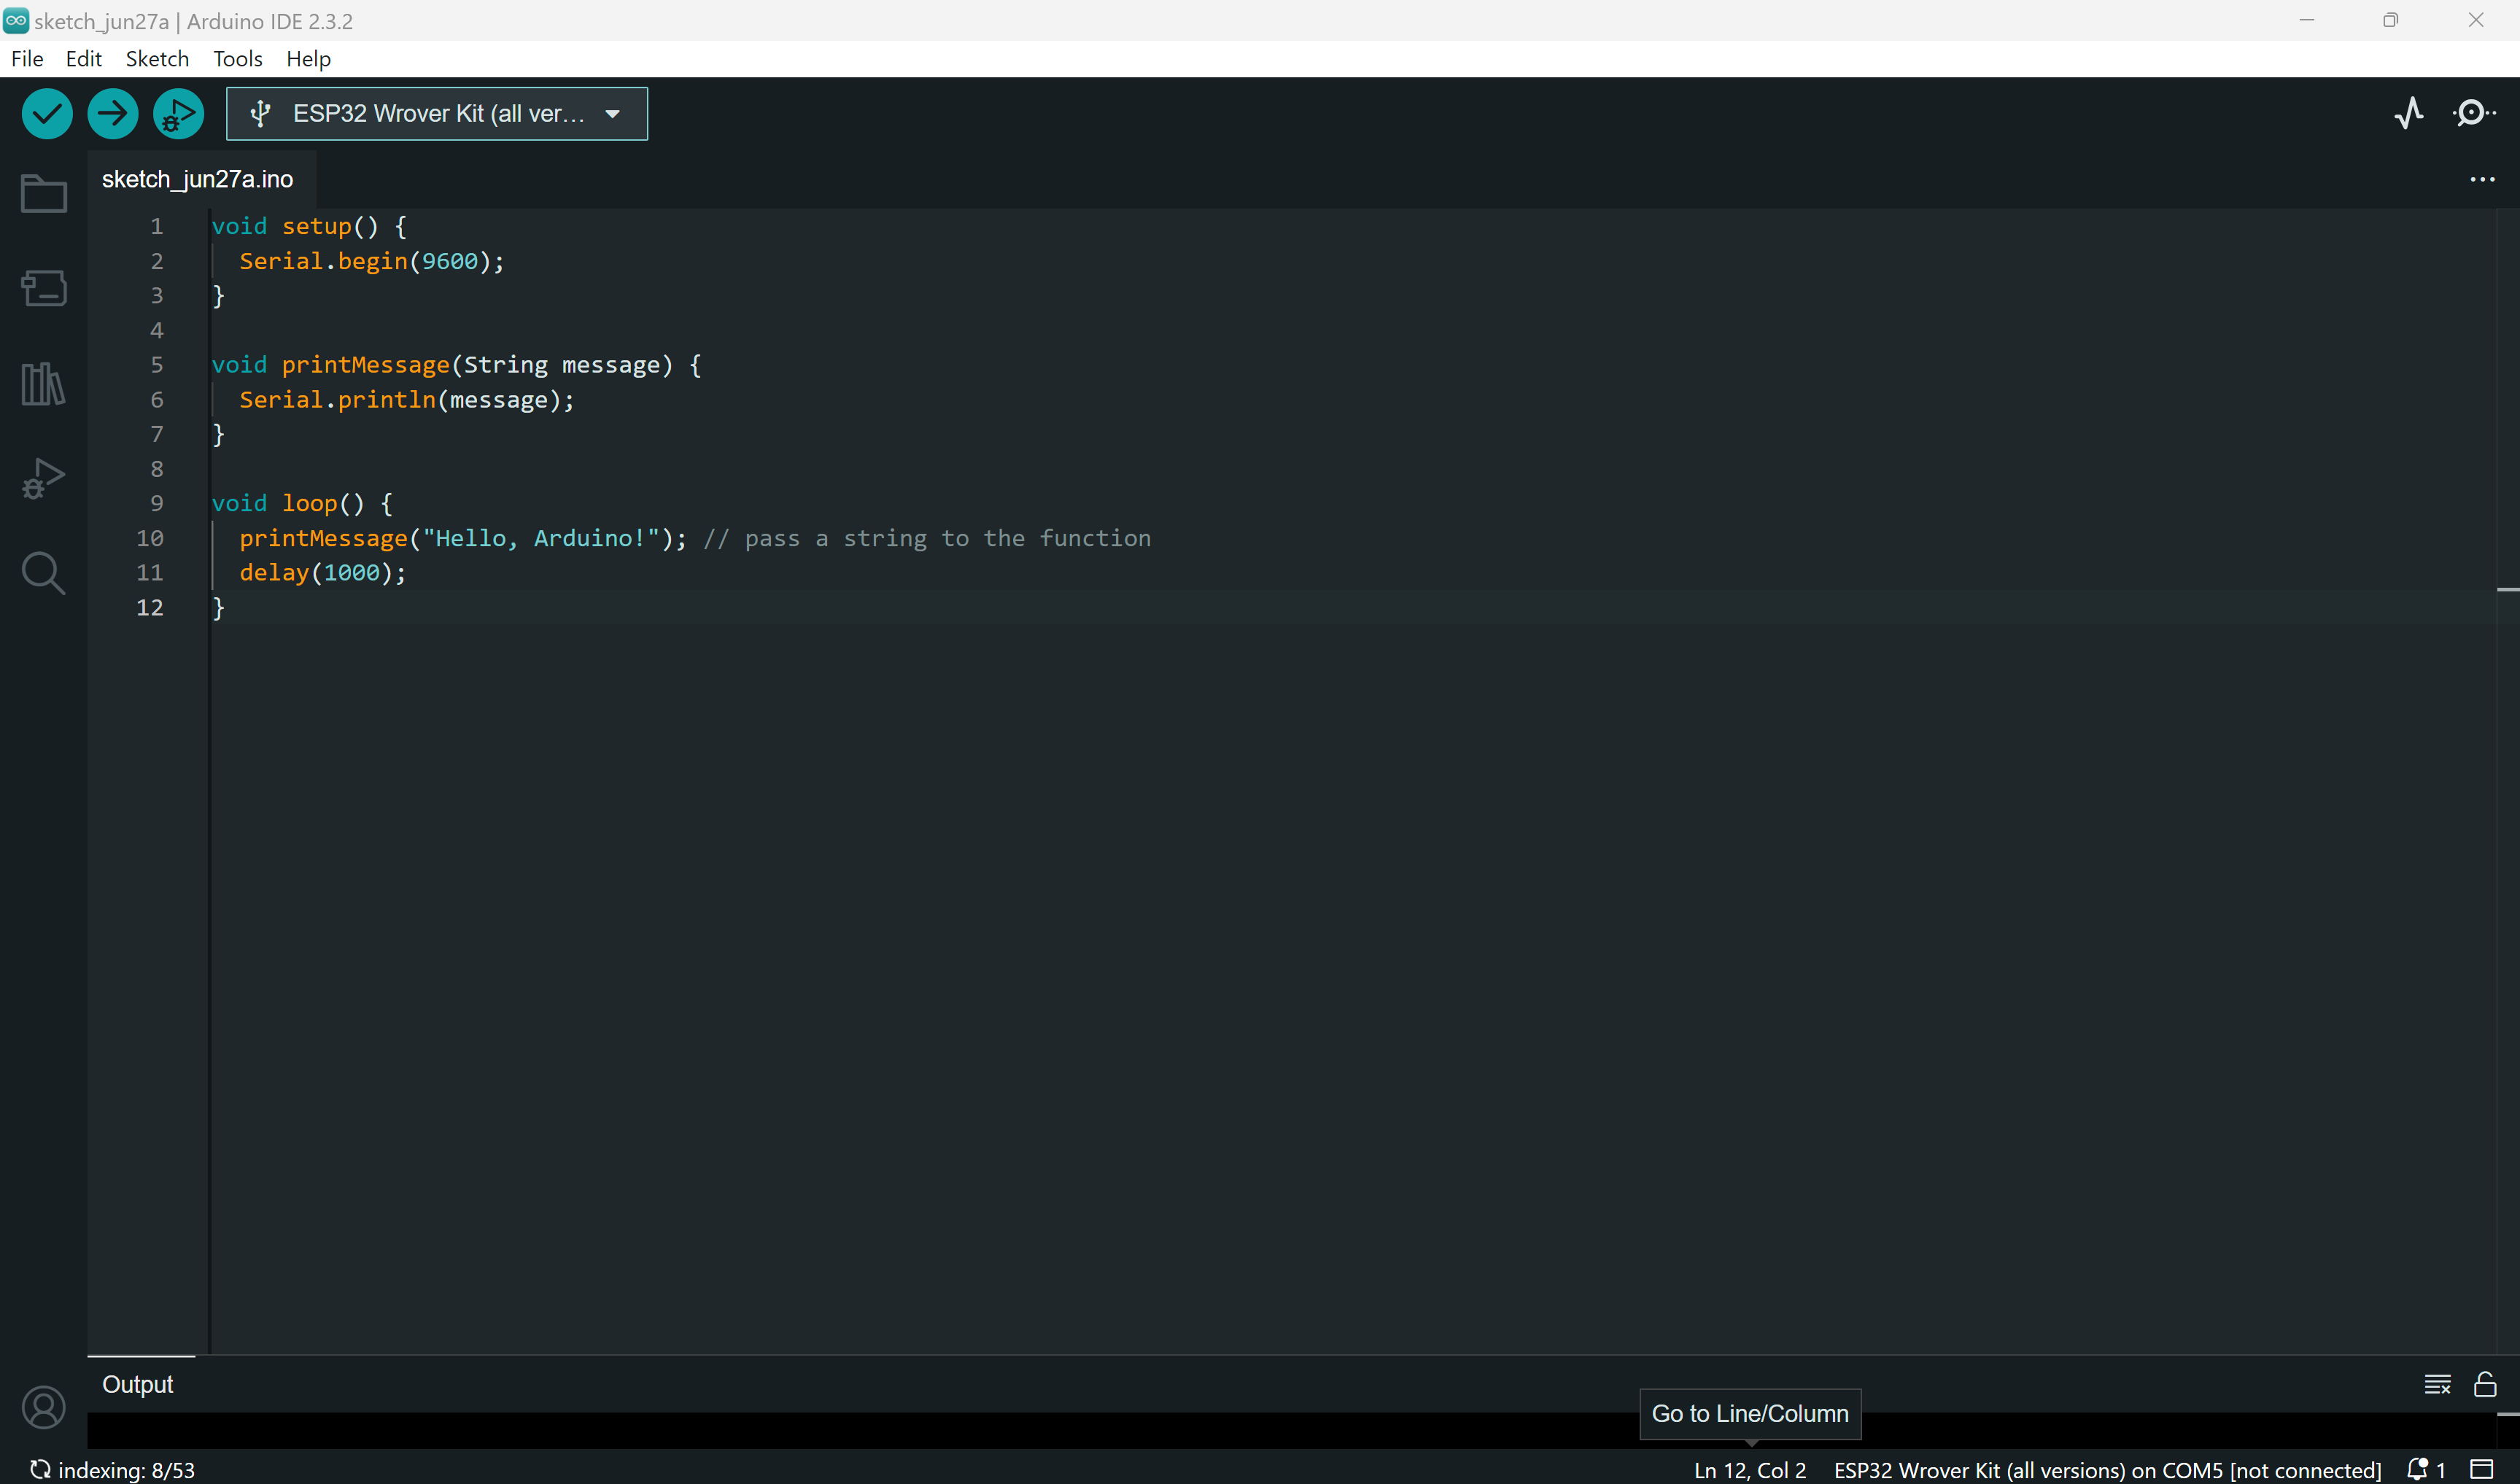
\includegraphics[width=\textwidth]{fig/fig12.png}
	\caption{C++ Function Parameters}
	\label{fig:12}
\end{figure}

\chapter{Arduino pins og special funktioner}
\section{pinMode i Arduino}
\textbf{pinMode()} funktionen i Arduino bruges til at konfigurere en specifik pin på mikrocontrolleren som enten en \textbf{input} eller \textbf{output}. Dette er et vigtigt skridt i opsætningen af hardware, da det bestemmer, hvordan en pin vil opføre sig under programkørslen. 
\newline\newline\noindent
Når en pin er konfigureret som \textbf{input}, kan den læse signaler fra sensorer eller knapper, hvilket betyder, at den kan modtage information fra omgivelserne. Når en pin er konfigureret som \textbf{output}, kan den sende signaler til komponenter som LED'er, motorer eller relæer, hvilket gør det muligt at styre disse enheder.

\begin{lstlisting}[language=C++, caption=Eksempel på brug af pinMode]
	void setup() {
		pinMode(13, OUTPUT);  // Sætter pin 13 som output (f.eks. til en LED)
		pinMode(7, INPUT);    // Sætter pin 7 som input (f.eks. til en knap)
	}
	
	void loop() {
		// Kode til at styre og læse fra pins
	}
\end{lstlisting}
I eksemplet ovenfor konfigureres pin 13 som en output, hvilket gør den velegnet til at tænde og slukke en LED. Pin 7 er konfigureret som input, hvilket gør den i stand til at læse signaler fra en knap. Dette er en grundlæggende, men afgørende funktion i Arduino-programmering, som giver brugeren kontrol over, hvordan mikrocontrolleren interagerer med eksterne komponenter.

\section{digitalRead og digitalWrite i Arduino}
\textbf{digitalRead()} og \textbf{digitalWrite()} er to essentielle funktioner i Arduino, der bruges til at læse og skrive digitale signaler på mikrocontrollerens pins.

\subsection{digitalRead()}
\textbf{digitalRead()} bruges til at læse statusen på en specificeret pin, som tidligere er sat op som \textbf{INPUT} med \texttt{pinMode()}. Denne funktion returnerer enten \texttt{HIGH} eller \texttt{LOW}, afhængigt af om der er spænding på pinnen (typisk 5V eller 3.3V for \texttt{HIGH}) eller ej (0V for \texttt{LOW}).
\begin{lstlisting}[language=C++, caption=Eksempel på brug af digitalRead]
	int buttonState = 0;
	
	void setup() {
		pinMode(7, INPUT);  // Sætter pin 7 som input
	}
	
	void loop() {
		buttonState = digitalRead(7);  // Læser tilstanden af pin 7
		if (buttonState == HIGH) {
			// Kode hvis knappen er trykket ned
		} else {
			// Kode hvis knappen ikke er trykket ned
		}
	}
\end{lstlisting}
I eksemplet ovenfor bruges \texttt{digitalRead()} til at afgøre, om en knap tilsluttet pin 7 er trykket ned (pinnen er \texttt{HIGH}) eller ej (\texttt{LOW}).

\subsection{digitalWrite()}
\textbf{digitalWrite()} bruges til at sætte en specifik pin til enten \texttt{HIGH} eller \texttt{LOW}. Dette gør det muligt at tænde eller slukke komponenter som LED'er, motorer eller relæer. For at bruge \texttt{digitalWrite()}, skal pinnen først være konfigureret som \textbf{OUTPUT} med \texttt{pinMode()}.

\begin{lstlisting}[language=C++, caption=Eksempel på brug af digitalWrite]
	void setup() {
		pinMode(13, OUTPUT);  // Sætter pin 13 som output
	}
	
	void loop() {
		digitalWrite(13, HIGH);   // Tænder LED tilsluttet pin 13
		delay(1000);              // Venter i 1 sekund
		digitalWrite(13, LOW);    // Slukker LED
		delay(1000);              // Venter i 1 sekund
	}
\end{lstlisting}
I eksemplet ovenfor bruges \texttt{digitalWrite()} til at tænde og slukke en LED tilsluttet pin 13. Funktionen skifter mellem \texttt{HIGH} (tænder LED'en) og \texttt{LOW} (slukker LED'en), med en forsinkelse på 1 sekund mellem hver skift.
\newline\newline\noindent
\textbf{digitalRead()} og \textbf{digitalWrite()} er grundlæggende byggesten i Arduino-programmering, da de giver kontrol over, hvordan mikrocontrolleren interagerer med digitale indgange og udgange.

\section{analogRead og analogWrite i Arduino}
\textbf{analogRead()} og \textbf{analogWrite()} er to funktioner i Arduino, der bruges til at læse og skrive analoge signaler på mikrocontrollerens pins.

\subsection{analogRead()}
\textbf{analogRead()} bruges til at læse værdien fra en analog indgangspin. Arduinoen har flere analoge indgange (typisk mærket som \texttt{A0}, \texttt{A1}, osv.), der kan læse spændinger mellem 0 og 5V (eller 0 og 3.3V afhængigt af modellen). Denne funktion returnerer en værdi mellem 0 og 1023, hvor 0 svarer til 0V og 1023 svarer til maksimal spænding.
\begin{lstlisting}[language=C++, caption=Eksempel på brug af analogRead]
	int sensorValue = 0;
	
	void setup() {
		Serial.begin(9600);  // Initialiserer seriel kommunikation
	}
	
	void loop() {
		sensorValue = analogRead(A0);  // Læser værdien fra pin A0
		Serial.println(sensorValue);   // Udskriver værdien til seriel monitor
		delay(500);                    // Venter i 0,5 sekunder
	}
\end{lstlisting}
I eksemplet ovenfor bruges \texttt{analogRead()} til at læse en spænding fra en sensor tilsluttet pin \texttt{A0}. Værdien udskrives derefter til seriel monitoren.

\subsection{analogWrite()}
\textbf{analogWrite()} bruges til at generere en pulsbreddemoduleret (PWM) signal på en specifik pin. Arduinoen har flere PWM-udgange (typisk markeret med en tilde, f.eks. \texttt{~3}, \texttt{~5}, osv.). Funktionen \texttt{analogWrite()} tager en værdi mellem 0 og 255, hvor 0 betyder ingen output (0V) og 255 betyder maksimal output (5V eller 3.3V, afhængigt af modellen).

\begin{lstlisting}[language=C++, caption=Eksempel på brug af analogWrite]
	int brightness = 0;
	
	void setup() {
		pinMode(9, OUTPUT);  // Sætter pin 9 som output
	}
	
	void loop() {
		for (brightness = 0; brightness <= 255; brightness++) {
			analogWrite(9, brightness);  // Justerer lysstyrken på LED'en
			delay(10);                   // Venter i 10 ms
		}
		for (brightness = 255; brightness >= 0; brightness--) {
			analogWrite(9, brightness);  // Justerer lysstyrken på LED'en
			delay(10);                   // Venter i 10 ms
		}
	}
\end{lstlisting}
I eksemplet ovenfor bruges \texttt{analogWrite()} til at kontrollere lysstyrken på en LED tilsluttet pin 9. Værdien varieres fra 0 (slukket) til 255 (maksimal lysstyrke) i en glidende overgang.
\newline\newline\noindent
\textbf{analogRead()} og \textbf{analogWrite()} er vigtige funktioner i Arduino-programmering, da de giver mulighed for at interagere med analoge signaler og justere output i forhold til en kontinuerlig skala.

\section{delay og millis i Arduino}
\textbf{delay()} og \textbf{millis()} er to funktioner i Arduino, der bruges til at arbejde med tid og timing i programmer.

\subsection{delay()}
\textbf{delay()} er en funktion, der forsinker udførelsen af programmet i et bestemt antal millisekunder. Funktionen stopper al kodeudførelse i det angivne tidsrum, hvilket kan være nyttigt, når du ønsker at skabe en simpel pause eller forsinkelse mellem handlinger.

\begin{lstlisting}[language=C++, caption=Eksempel på brug af delay]
	void setup() {
		pinMode(13, OUTPUT);  // Sætter pin 13 som output
	}
	
	void loop() {
		digitalWrite(13, HIGH);  // Tænder LED'en tilsluttet pin 13
		delay(1000);             // Venter i 1000 ms (1 sekund)
		digitalWrite(13, LOW);   // Slukker LED'en
		delay(1000);             // Venter i 1000 ms (1 sekund)
	}
\end{lstlisting}
I eksemplet ovenfor bruges \texttt{delay()} til at skabe en 1-sekunds pause, hvor en LED tændes og slukkes skiftevis. Det er en enkel måde at styre tid i dit program på, men det blokerer programudførelsen, hvilket betyder, at ingen anden kode kan køre, mens \texttt{delay()} udføres.

\subsection{millis()}
\textbf{millis()} er en funktion, der returnerer antallet af millisekunder, der er gået, siden Arduinoen startede. Funktionen bruges ofte til at udføre tidstagning uden at blokere programudførelsen, hvilket gør den ideel til opgaver, der kræver nøjagtig timing uden at stoppe al anden kodeudførelse.
\begin{lstlisting}[language=C++, caption=Eksempel på brug af millis]
	unsigned long previousMillis = 0;
	const long interval = 1000;  // Intervallet er sat til 1000 ms (1 sekund)
	
	void setup() {
		pinMode(13, OUTPUT);  // Sætter pin 13 som output
	}
	
	void loop() {
		unsigned long currentMillis = millis();
		
		if (currentMillis - previousMillis >= interval) {
			previousMillis = currentMillis;  // Opdaterer tidligere tid
			digitalWrite(13, !digitalRead(13));  // Skifter LED'ens tilstand
		}
	}
\end{lstlisting}
I eksemplet ovenfor bruges \texttt{millis()} til at blinke en LED uden at blokere programudførelsen. LED'en skifter tilstand (tændt/slukket) hver gang intervallet på 1 sekund er gået. Fordelen ved \texttt{millis()} er, at det tillader andre funktioner i \texttt{loop()} at køre samtidigt, hvilket er vigtigt i komplekse programmer, hvor flere opgaver skal udføres parallelt.
\newline\newline\noindent
\textbf{delay()} er enkel og nem at bruge, men den stopper programmet midlertidigt, hvilket kan være uønsket i mere avancerede applikationer. \textbf{millis()} giver en mere fleksibel måde at håndtere tid og timing på uden at stoppe andre dele af programmet, hvilket gør det til et foretrukket valg i mange tilfælde.



%	C++ Advanced
	\part{C++ advanced}
\chapter{C++ Advanced}
\section{C++ Classes}
\textbf{Formål:} Dette afsnit introducerer objektorienteret programmering (OOP) i C++, herunder klasser, objekter, metoder, Constructors, access specifiers, encapsulation, arv og polymorfisme. Studerende vil lære at bruge OOP-koncepter til at skrive mere struktureret og genanvendelig kode til Arduino-projekter.
\\\\
\noindent\textbf{Læringsmål:} Efter at have læst dette afsnit forventes det, at studerende kan:
\begin{itemize}
	\item Forstå grundlæggende OOP-konceptet og dets anvendelse i Arduino.
	\item Definere og bruge klasser og objekter i Arduino-kode.
	\item Implementere klassemetoder og Constructors i Arduino.
	\item Bruge access specifiers til at kontrollere adgang til klassemedlemmer i Arduino.
	\item Forstå og anvende encapsulation i Arduino-projekter.
	\item Implementere arv og polymorfisme i deres Arduino-programmer.
\end{itemize}

\subsection{C++ Classes/Objects}
\textbf{Teori:} Klasser og objekter er grundlæggende byggesten i objektorienteret programmering (OOP). En klasse er en skabelon eller blueprint for objekter, som definerer de attributter (variabler) og metoder (funktioner), objekterne skal have. En klasse repræsenterer en abstraktion af en ting, hvor tingene har fælles egenskaber og adfærd. Et objekt er en instans af en klasse, hvilket betyder, at det er en konkret manifestation af klassen med specifikke værdier for dets attributter.
\\\\
\noindent OOP gør det muligt at modellere virkelige objekter og deres adfærd på en måde, der gør koden mere struktureret og genanvendelig. Ved at bruge klasser og objekter kan programmører opdele komplekse problemer i mindre, håndterbare enheder, hvilket letter både udvikling og vedligeholdelse af koden.
\\\\
\noindent\noindent\textbf{Eksempel:}
\begin{lstlisting}[language=C++]
	class LED {
		int pin;
		
		public:
		LED(int p) {
			pin = p;
			pinMode(pin, OUTPUT);
		}
		
		void on() {
			digitalWrite(pin, HIGH);
		}
		
		void off() {
			digitalWrite(pin, LOW);
		}
	};
	
	LED led1(13); // create an object of class LED
	
	void setup() {
	}
	
	void loop() {
		led1.on();
		delay(1000);
		led1.off();
		delay(1000);
	}
\end{lstlisting}
\begin{figure}[h!]
	\centering
	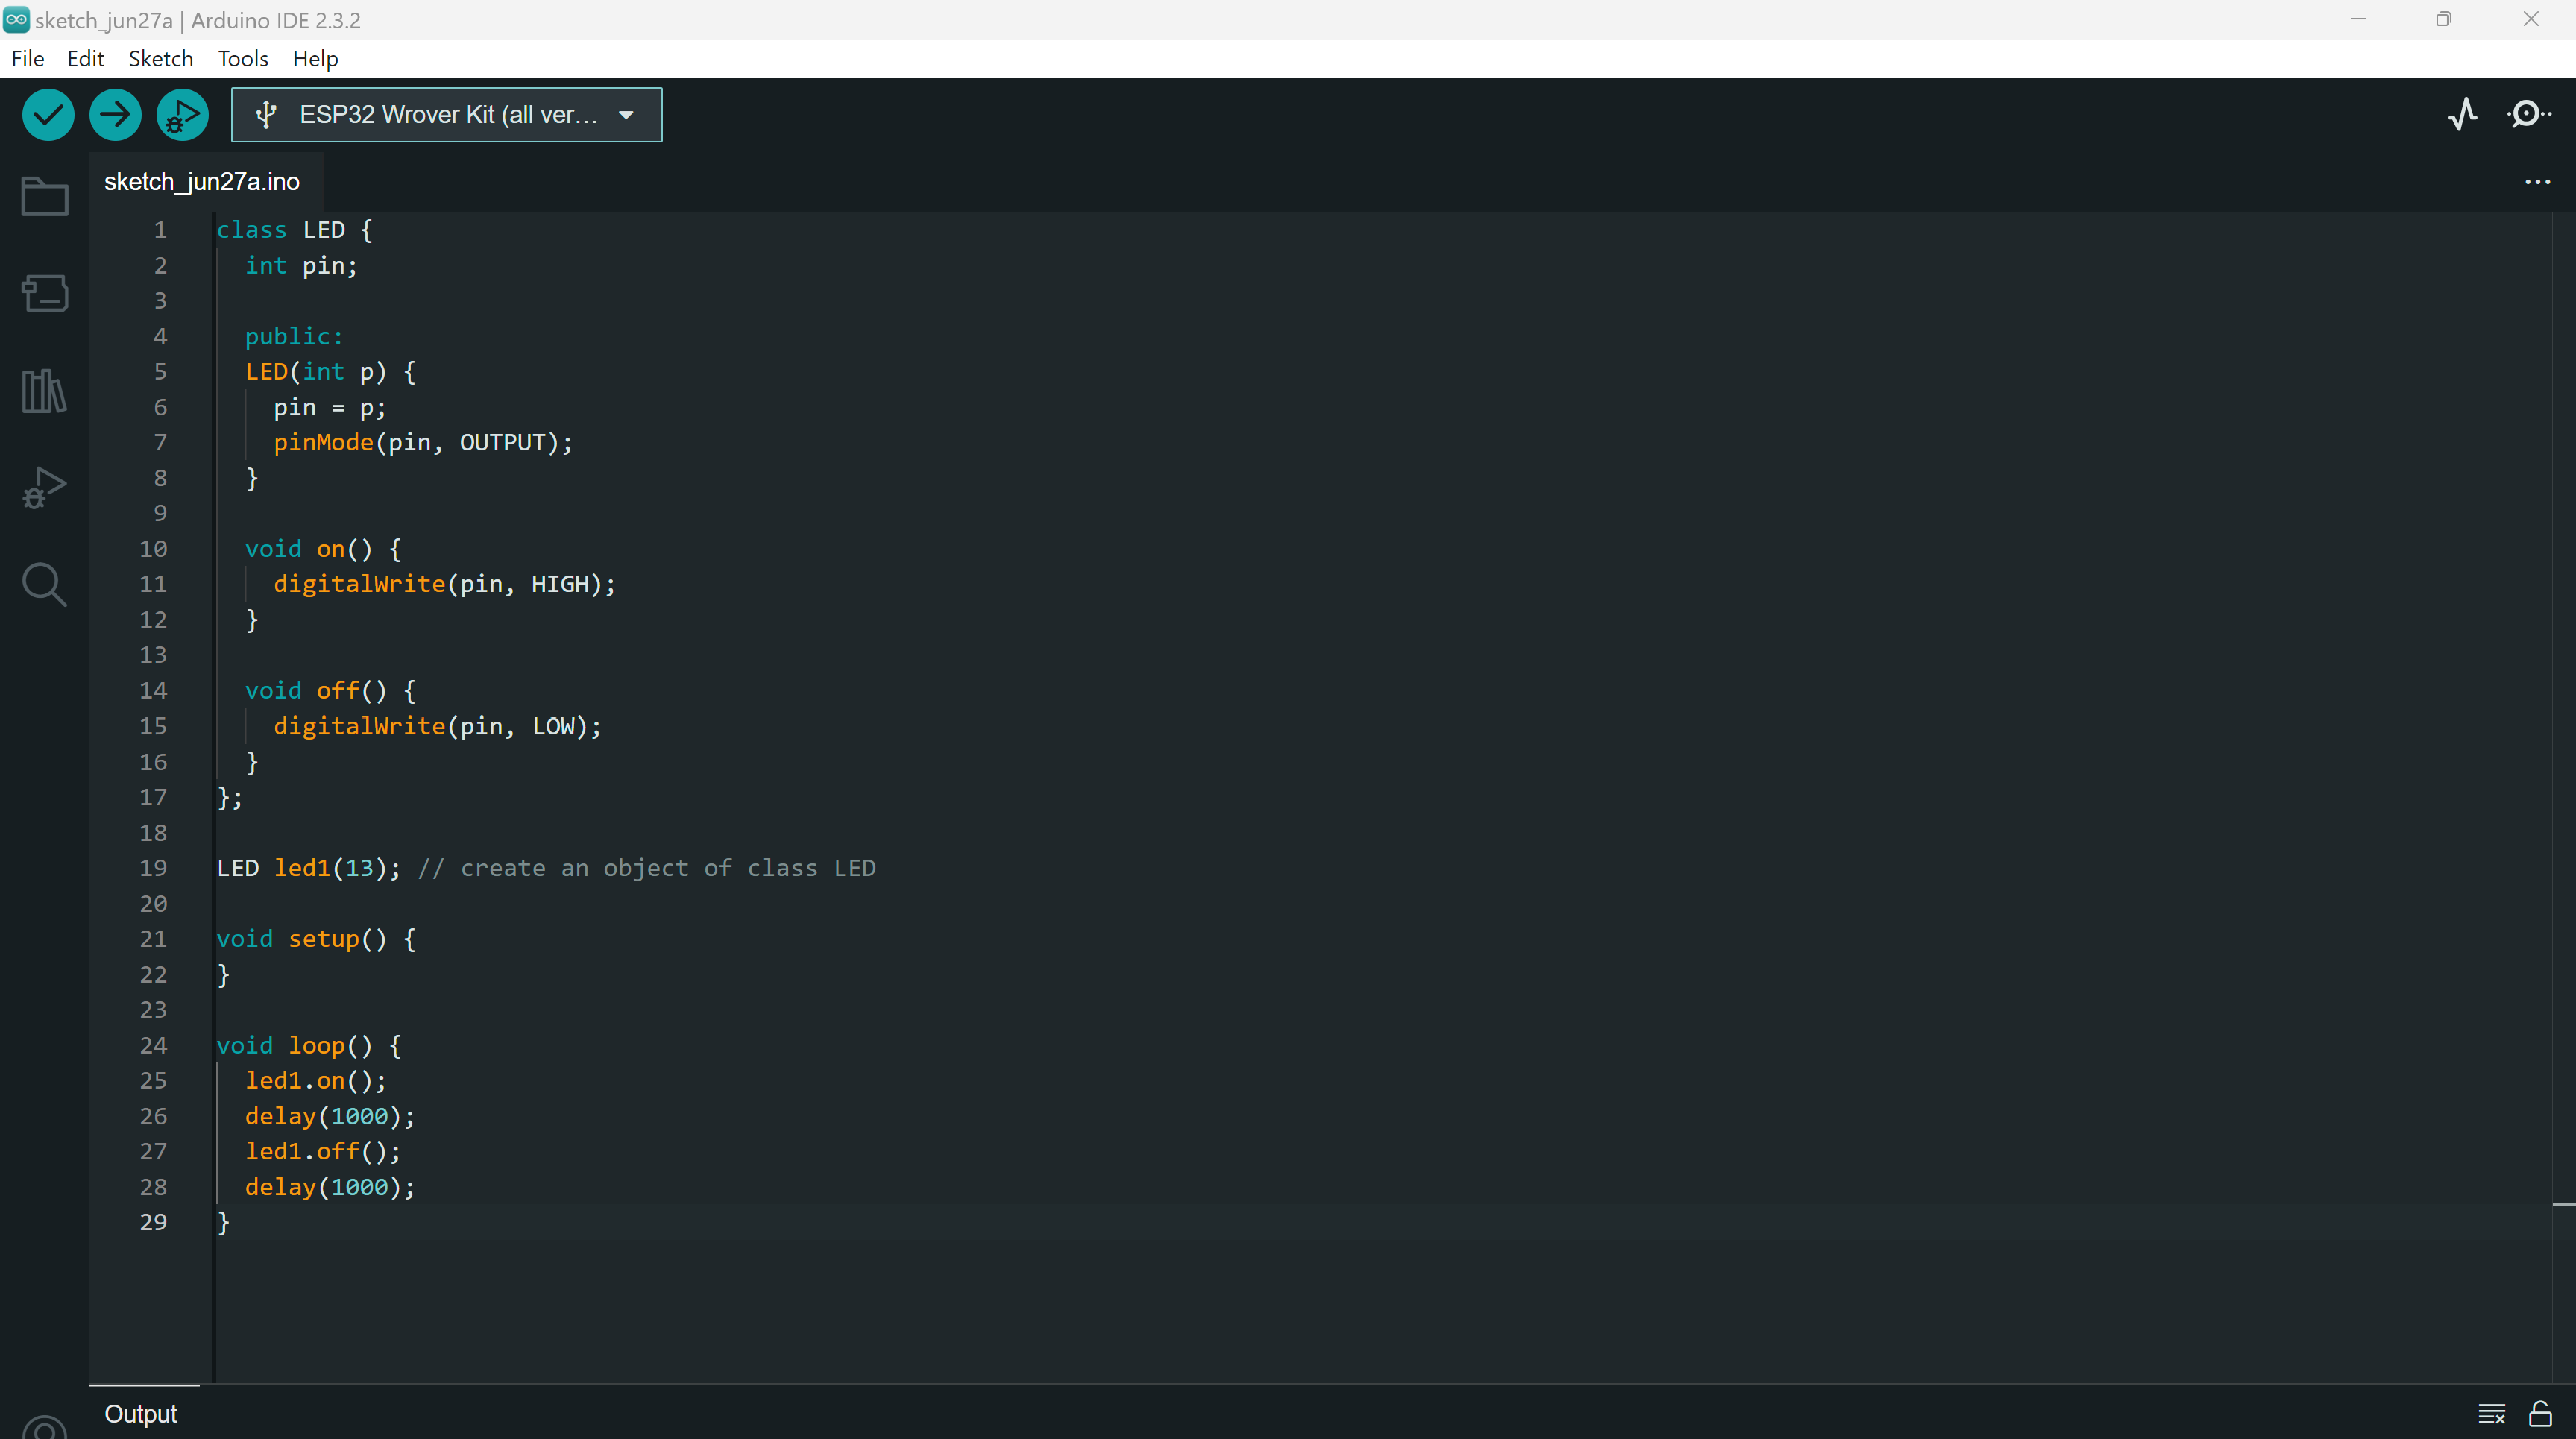
\includegraphics[width=\textwidth]{fig/fig13.png}
	\caption{text}
	\label{fig:13}
\end{figure}

\subsection{C++ Class Methods}
\textbf{Teori:} Metoder er funktioner, der er defineret inde i en klasse. De bruges til at definere adfærd for objekter. Metoder kan manipulere objektets tilstand og udføre opgaver baseret på objektets data. Metoder kan have adgang til objektets data via \texttt{this} pegeren, som implicit henviser til det kaldende objekt.
\\\\
\noindent Metoder kan være offentlige (\texttt{public}) eller private (\texttt{private}), hvilket kontrollerer deres synlighed og adgang fra udenfor klassen. Offentlige metoder er en del af klassens offentlige grænseflade, mens private metoder kun kan kaldes fra indenfor klassen selv.
\\\\
\noindent\textbf{Eksempel:}
\begin{lstlisting}[language=C++]
	class LED {
		int pin;
		
		public:
		LED(int p) {
			pin = p;
			pinMode(pin, OUTPUT);
		}
		
		void on() {
			digitalWrite(pin, HIGH);
		}
		
		void off() {
			digitalWrite(pin, LOW);
		}
	};
	
	LED led1(13);
	
	void setup() {
	}
	
	void loop() {
		led1.on();
		delay(1000);
		led1.off();
		delay(1000);
	}
\end{lstlisting}
\begin{figure}[h!]
	\centering
	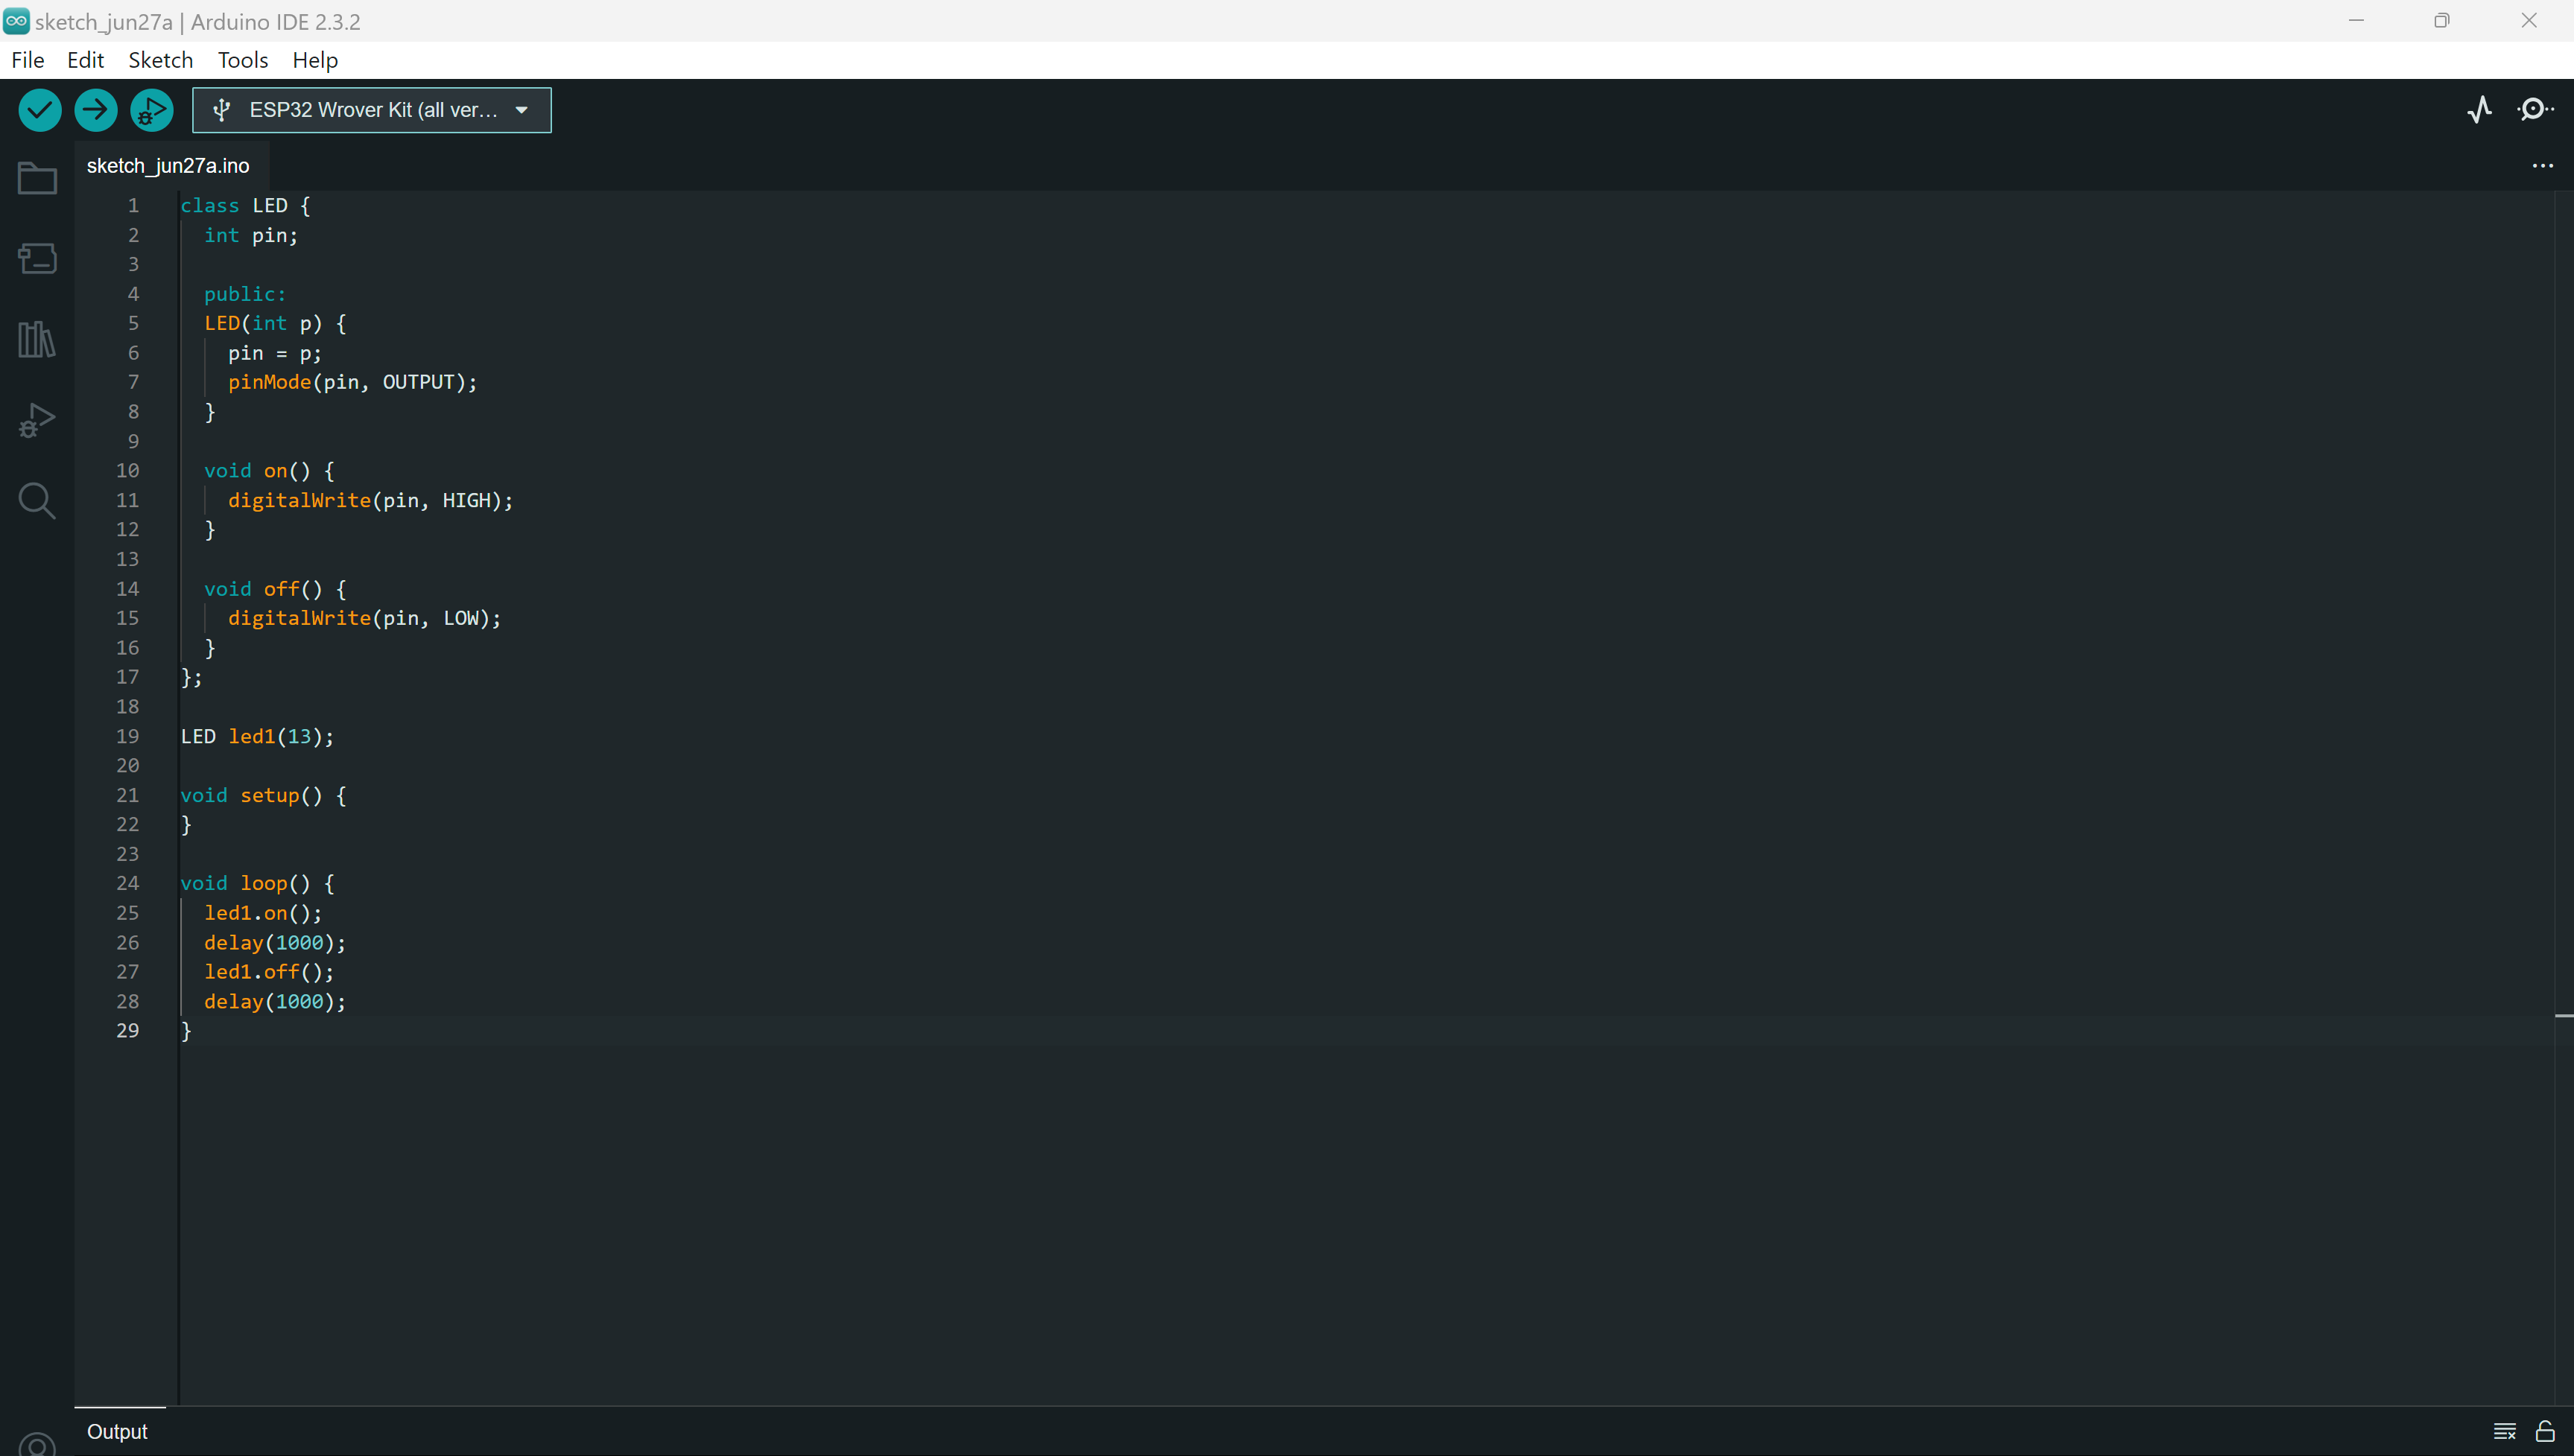
\includegraphics[width=\textwidth]{fig/fig18.png}
	\caption{C++ Class Methods}
	\label{fig:18}
\end{figure}


\subsection{C++ Constructors}
\textbf{Teori:} Constructors er specielle metoder, der kaldes automatisk, når et objekt skabes. De bruges til at initialisere objektets egenskaber. Constructors har samme navn som klassen og har ingen returtype. Constructors kan også tage parametre, som kan bruges til at initialisere objektets data med specifikke værdier ved skabelsen.
\\\\
\noindent En korrekt brug af Constructors er vigtig for at sikre, at objekter altid starter i en gyldig tilstand. Desuden kan Constructors også bruges til at allokere ressourcer, som objektet har brug for i sin levetid.
\\\\
\noindent\textbf{Eksempel:}
\begin{lstlisting}[language=C++]
	class LED {
		int pin;
		
		public:
		LED(int p) {
			pin = p;
			pinMode(pin, OUTPUT);
		}
		
		void on() {
			digitalWrite(pin, HIGH);
		}
		
		void off() {
			digitalWrite(pin, LOW);
		}
	};
	
	LED led1(13); // constructor is called here
	
	void setup() {
	}
	
	void loop() {
		led1.on();
		delay(1000);
		led1.off();
		delay(1000);
	}
\end{lstlisting}
\begin{figure}[h!]
	\centering
	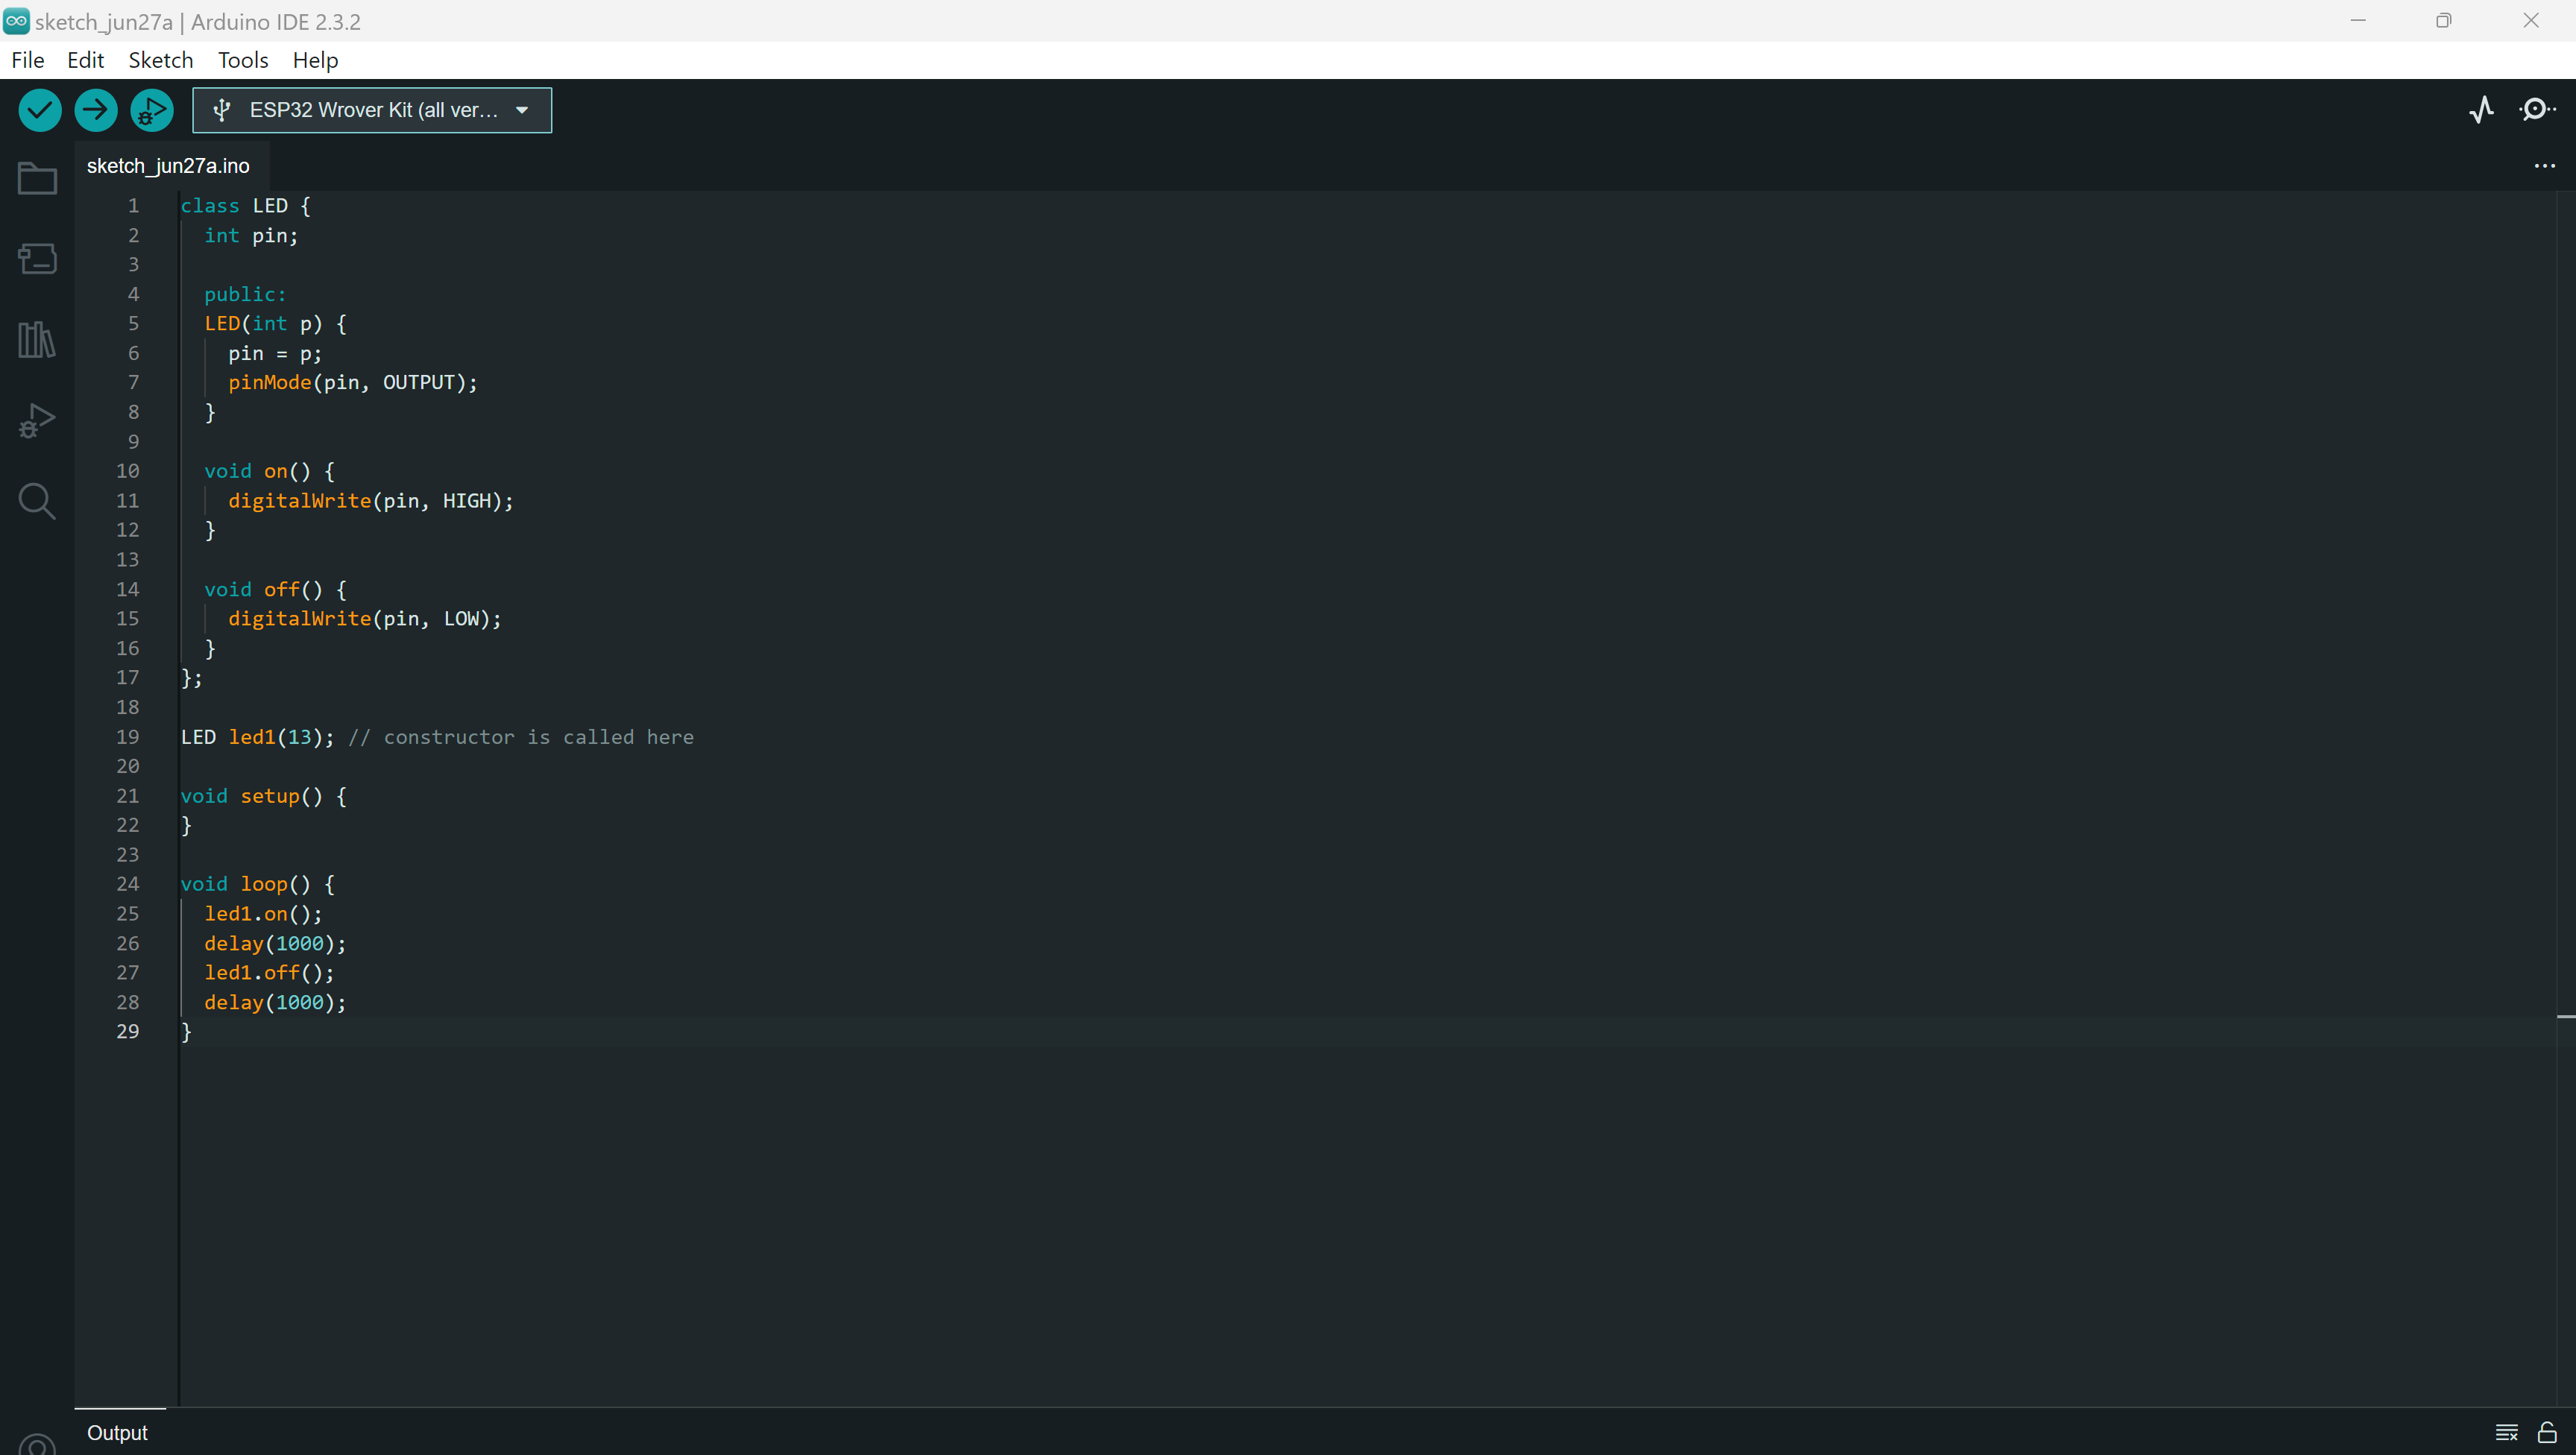
\includegraphics[width=\textwidth]{fig/fig17.png}
	\caption{C++ Constructors}
	\label{fig:17}
\end{figure}

\subsection{C++ Access Specifiers}
\textbf{Teori:} Access specifiers kontrollerer adgangen til klassemedlemmer. De mest almindelige access specifiers er \texttt{public}, \texttt{private}, og \texttt{protected}. \texttt{public} medlemmer kan tilgås fra enhver kode, mens \texttt{private} medlemmer kun kan tilgås fra indenfor klassen selv. \texttt{protected} medlemmer kan tilgås fra klassen og dens subklasser, men ikke fra andre dele af programmet.
\\\\
\noindent Access specifiers er en vigtig del af encapsulation, en OOP-praksis, der hjælper med at beskytte data og funktioner inde i en klasse fra utilsigtet eller skadelig adgang og ændring.
\\\\
\noindent\noindent\textbf{Eksempel:}
\begin{lstlisting}[language=C++]
	class LED {
		private:
		int pin;
		
		public:
		LED(int p) {
			pin = p;
			pinMode(pin, OUTPUT);
		}
		
		void on() {
			digitalWrite(pin, HIGH);
		}
		
		void off() {
			digitalWrite(pin, LOW);
		}
	};
	
	LED led1(13);
	
	void setup() {
	}
	
	void loop() {
		led1.on();
		delay(1000);
		led1.off();
		delay(1000);
	}
\end{lstlisting}
\begin{figure}[h!]
	\centering
	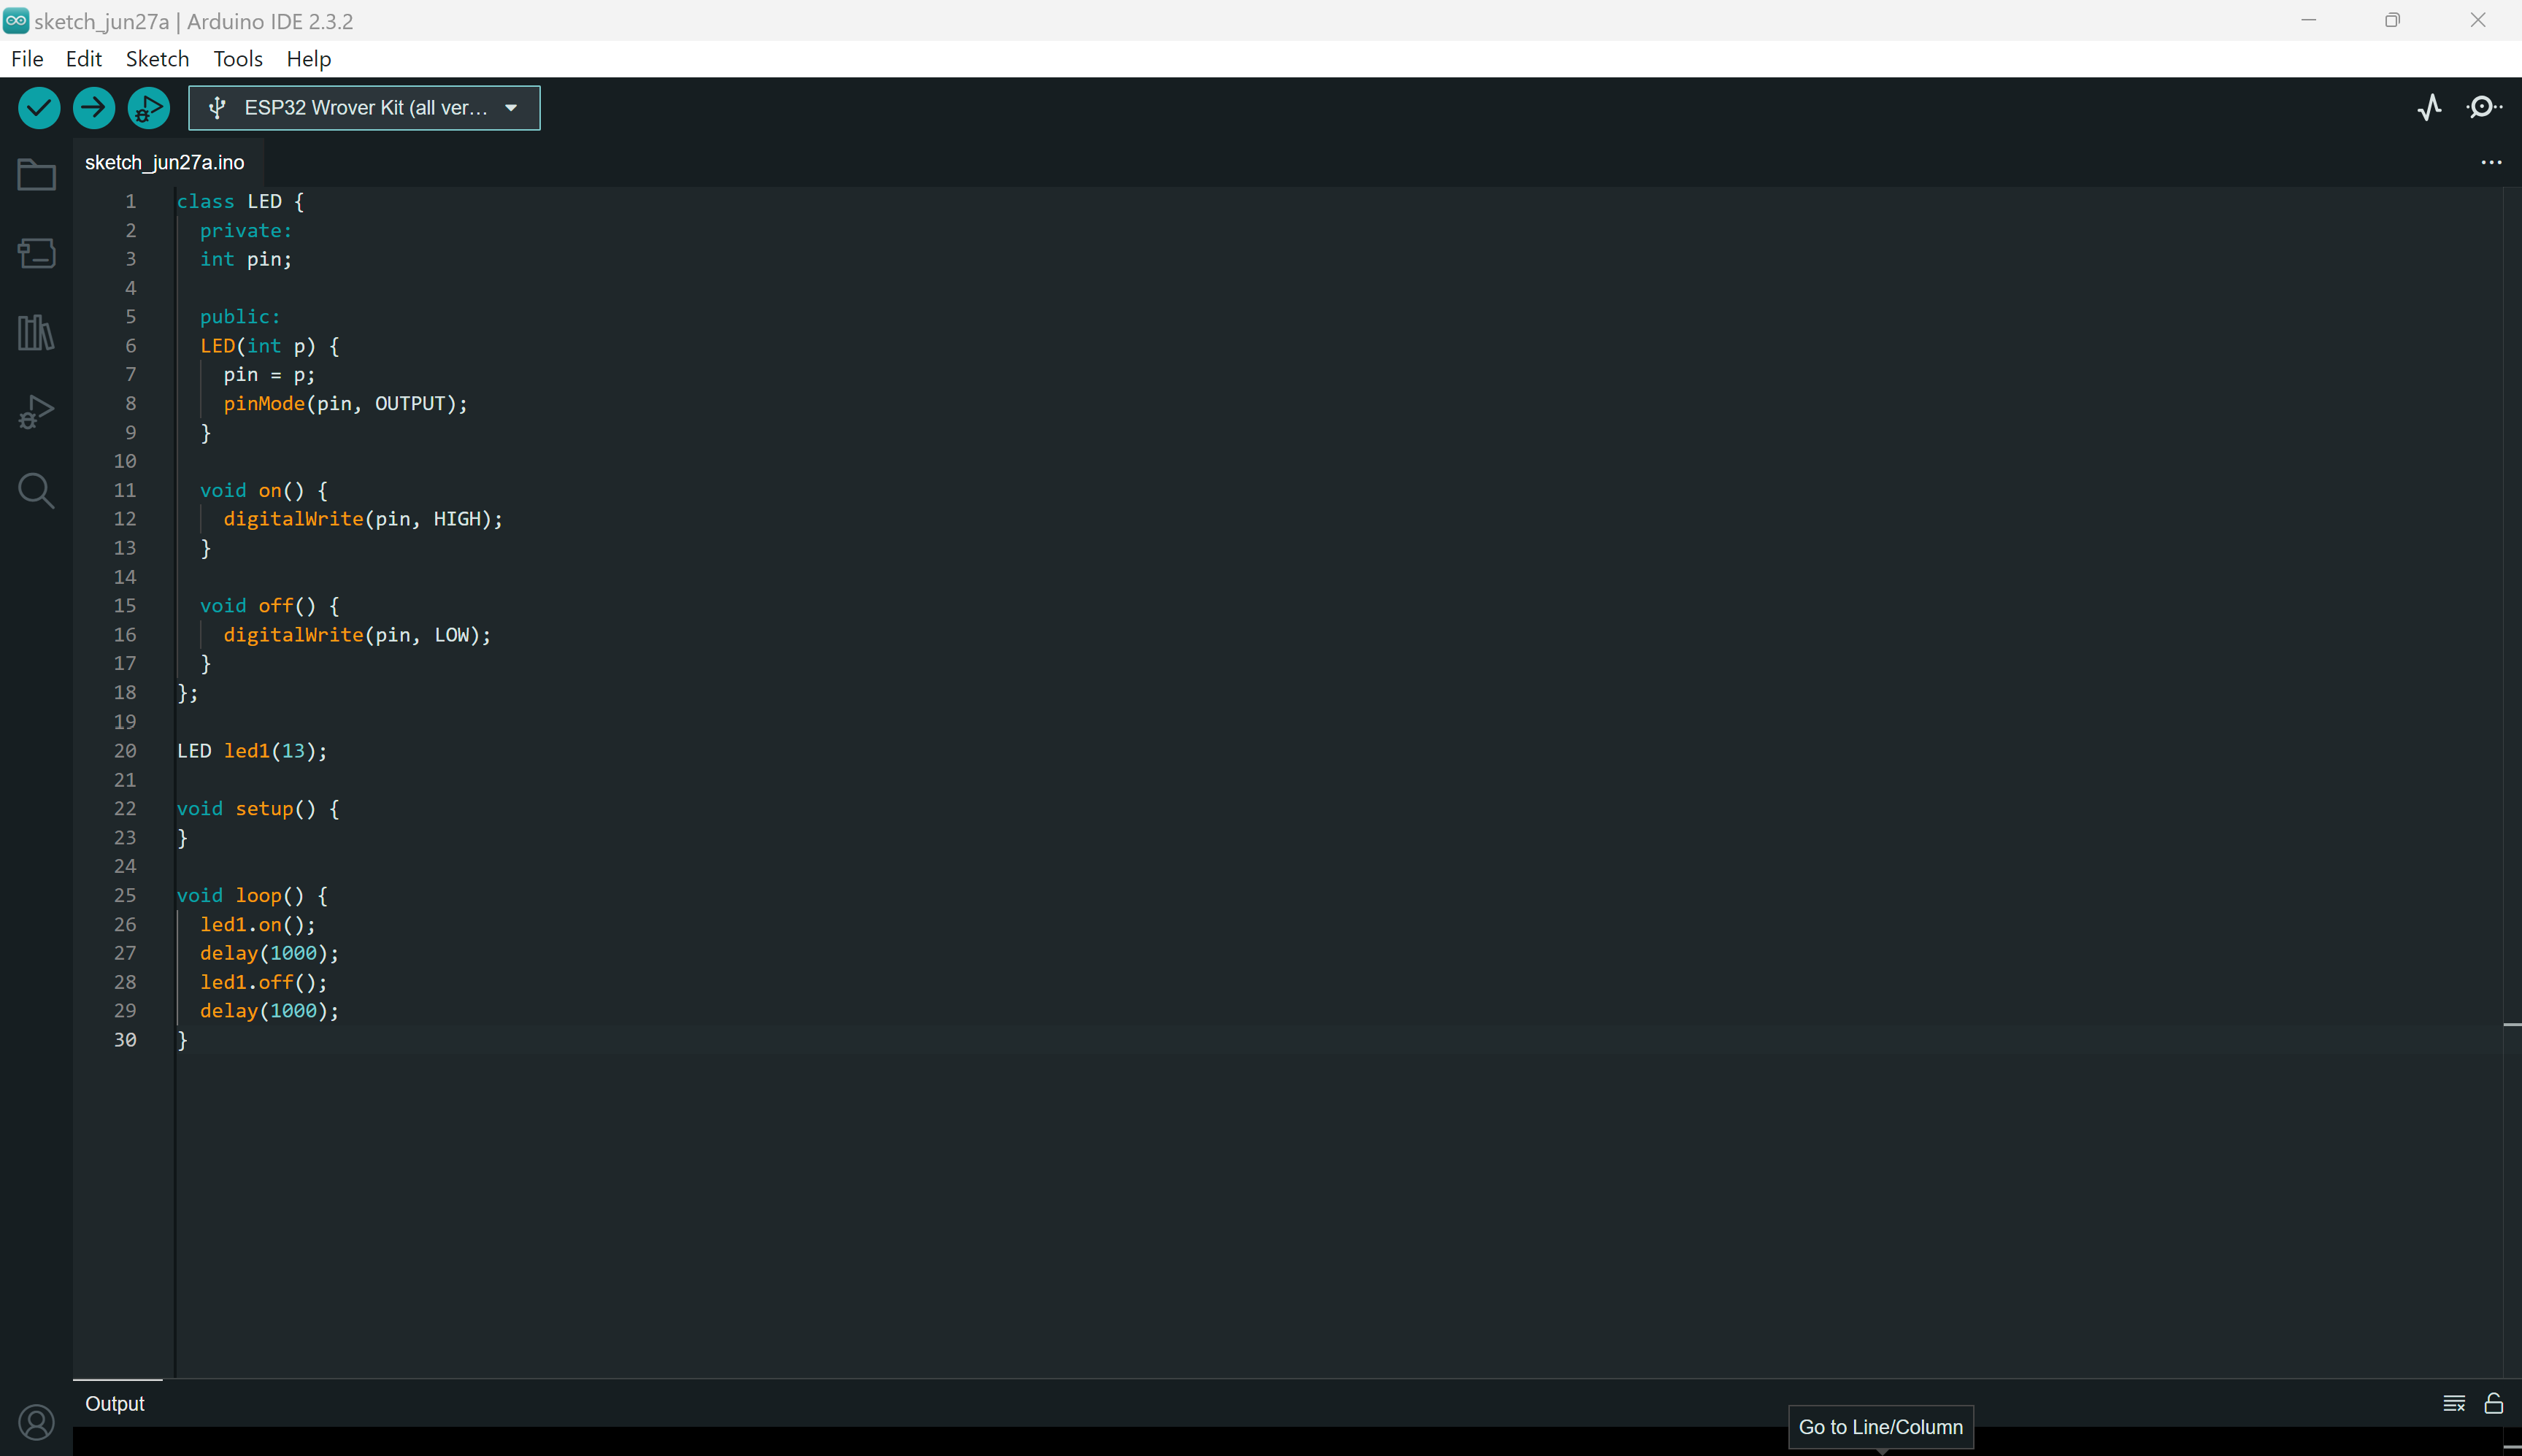
\includegraphics[width=\textwidth]{fig/fig16.png}
	\caption{C++ Access Specifiers}
	\label{fig:16}
\end{figure}

\subsection{C++ Encapsulation}
\textbf{Teori:} Encapsulation er processen med at skjule data implementeringsdetaljer og beskytte mod uautoriseret adgang. Det opnås ved hjælp af private medlemmer og offentlige metoder. Encapsulation sikrer data integritet og gør koden mere robust og vedligeholdelsesvenlig. Ved at skjule objektets indre detaljer kan udviklere ændre implementeringen uden at påvirke andre dele af programmet, som afhænger af objektets grænseflade.
\\\\
\noindent Encapsulation gør det muligt at skabe en klar og veldefineret grænseflade for en klasse, hvilket gør det lettere at bruge og forstå klassen uden at kende dens indre detaljer. Det fremmer også genbrug af kode og modularitet.
\\\\
\noindent\noindent\textbf{Eksempel:}
\begin{lstlisting}[language=C++]
	class LED {
		private:
		int pin;
		
		public:
		LED(int p) {
			pin = p;
			pinMode(pin, OUTPUT);
		}
		
		void on() {
			digitalWrite(pin, HIGH);
		}
		
		void off() {
			digitalWrite(pin, LOW);
		}
	};
	
	LED led1(13);
	
	void setup() {
	}
	
	void loop() {
		led1.on();
		delay(1000);
		led1.off();
		delay(1000);
	}
\end{lstlisting}
\begin{figure}[h!]
	\centering
	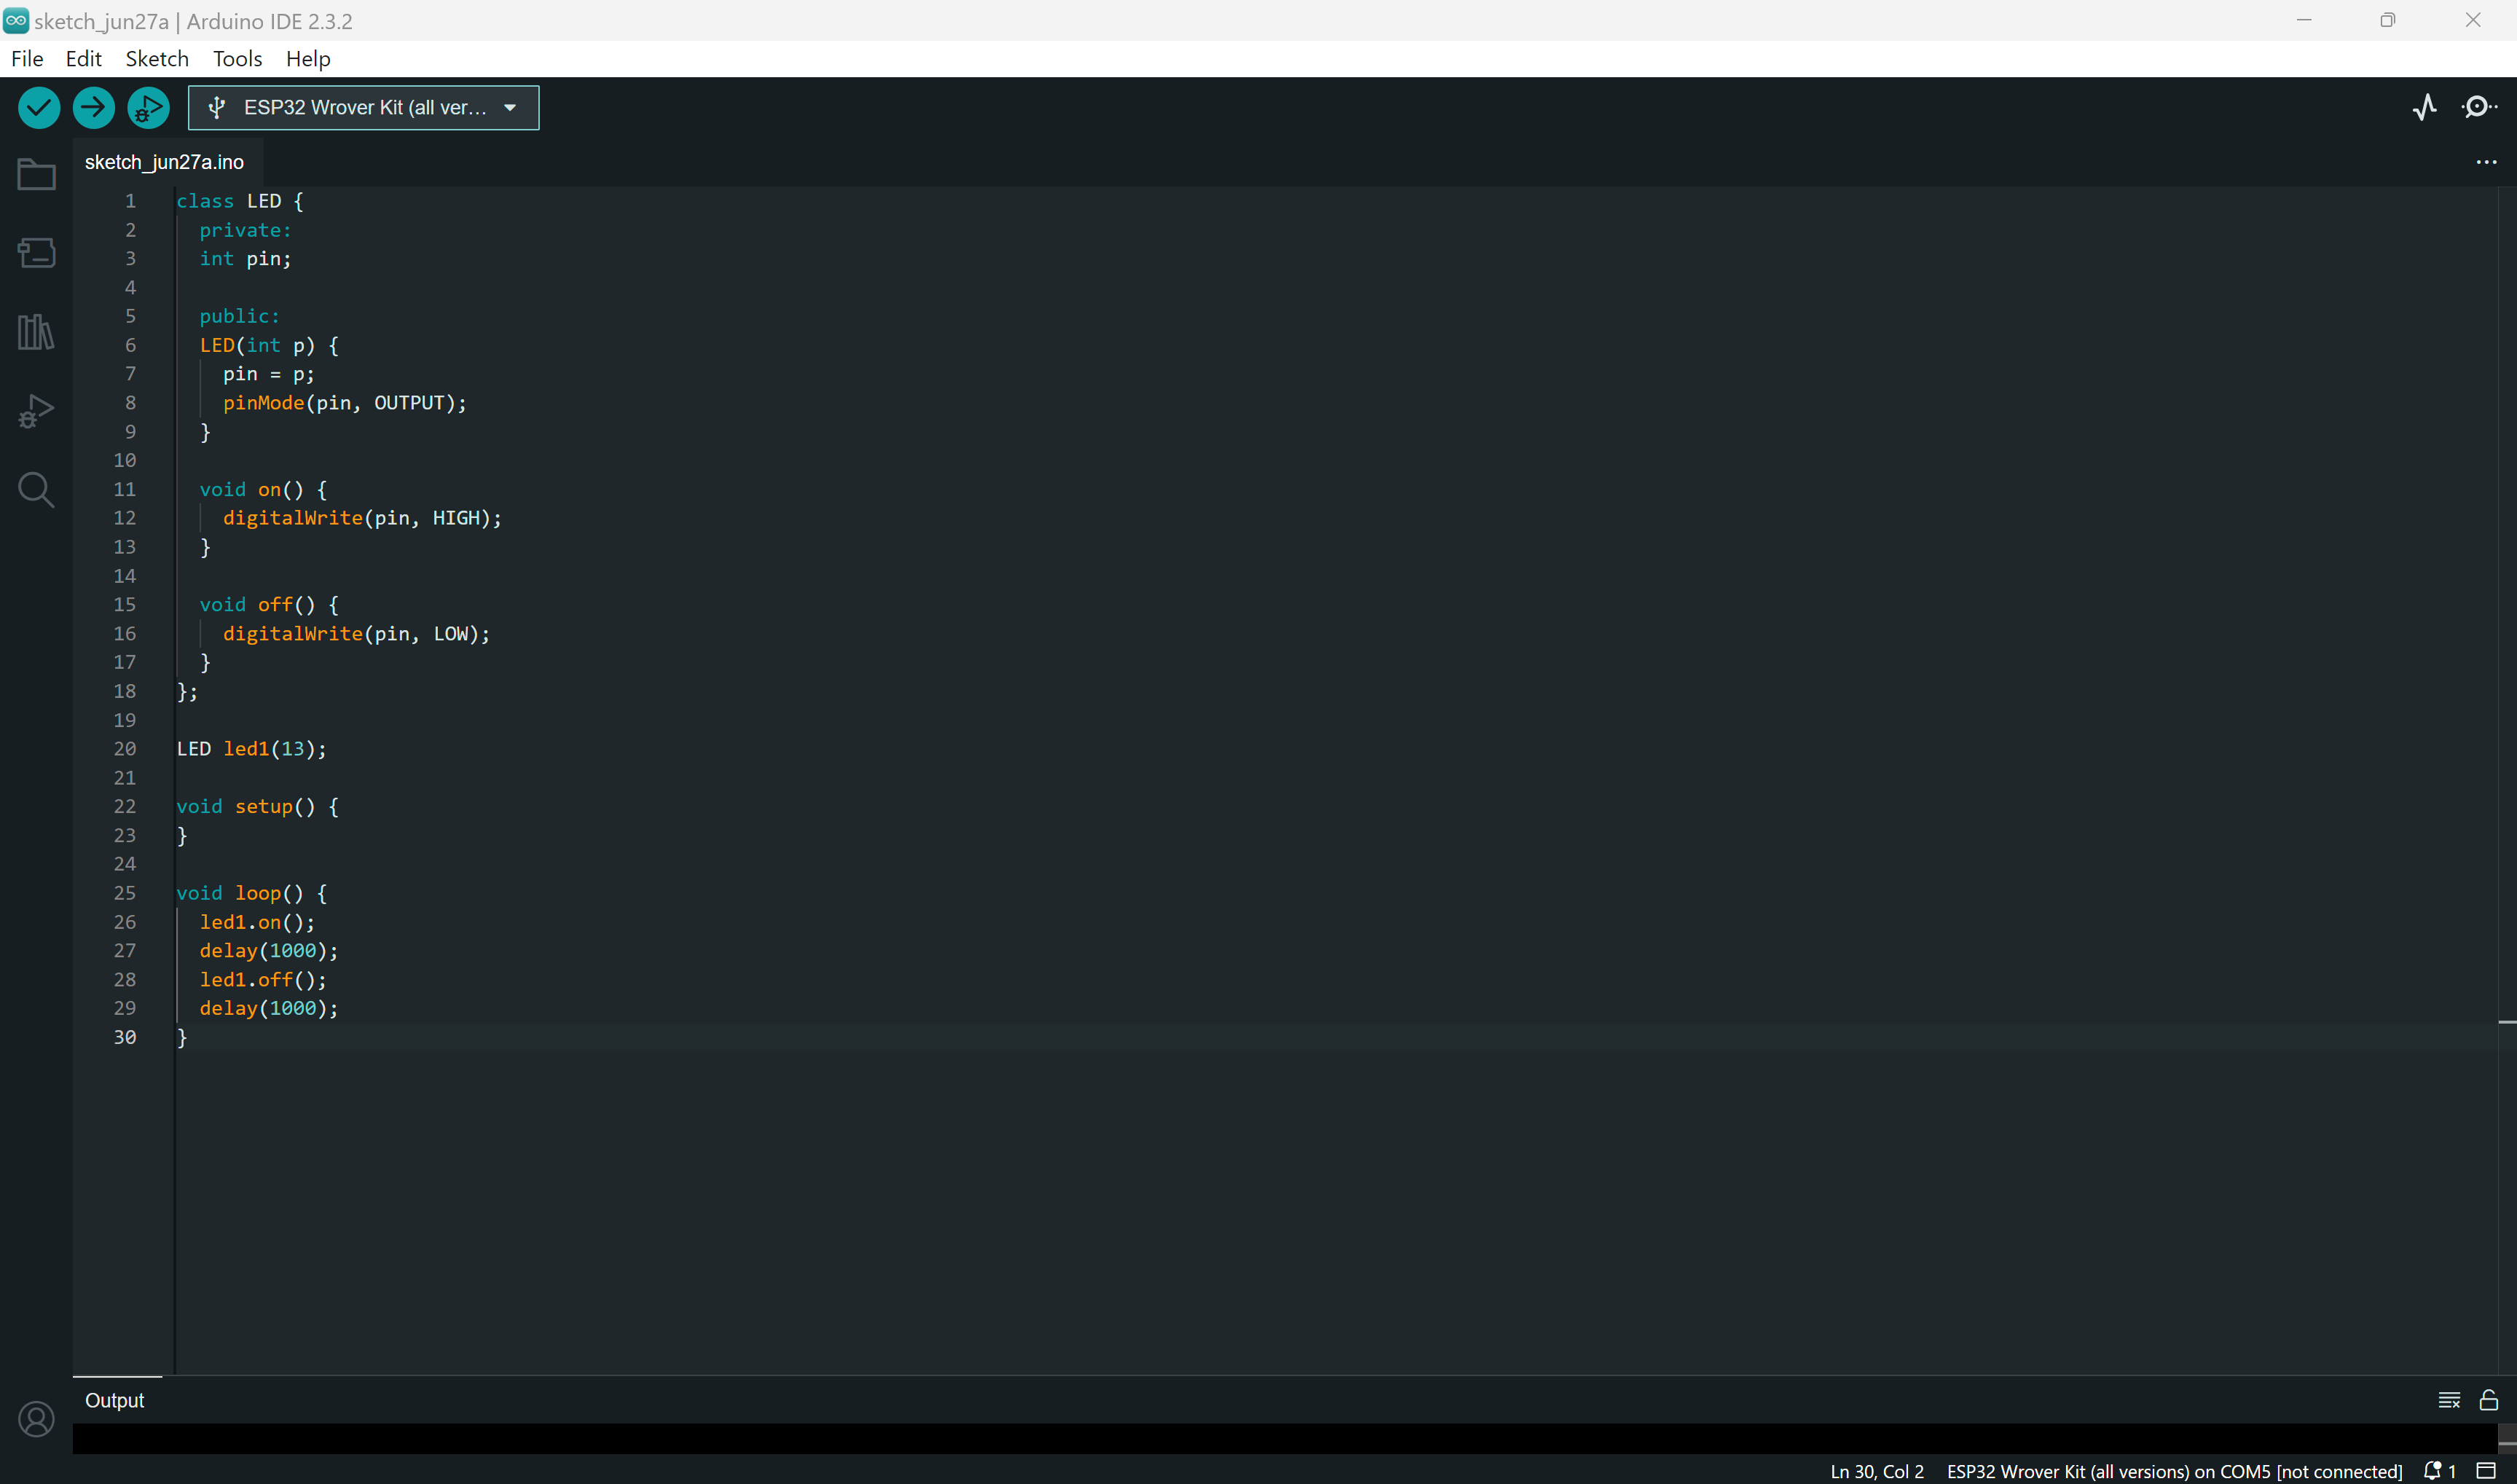
\includegraphics[width=\textwidth]{fig/fig15.png}
	\caption{C++ Encapsulation}
	\label{fig:15}
\end{figure}

\subsection{C++ Inheritance}
\textbf{Teori:} Arv tillader en klasse at arve egenskaber og metoder fra en anden klasse. Dette fremmer genbrug og struktureret kode. En baseklasse (eller superklasse) kan have flere afledte klasser (eller subklasser), som nedarver baseklassens medlemmer og metoder. Afledte klasser kan også tilføje deres egne medlemmer og metoder eller overskrive baseklassens metoder.
\\\\
\noindent Arv bruges til at skabe en hierarkisk struktur og dele funktionalitet på tværs af klasser. Det tillader udviklere at bygge komplekse systemer ved at genbruge og udvide eksisterende kode. Arv understøtter også polymorfisme, hvor objekter af forskellige klasser kan behandles ens, hvis de deler samme baseklasse.
\\\\
\noindent\textbf{Eksempel:}
\begin{lstlisting}[language=C++]
	class LED {
		protected:
		int pin;
		
		public:
		LED(int p) {
			pin = p;
			pinMode(pin, OUTPUT);
		}
		
		void on() {
			digitalWrite(pin, HIGH);
		}
		
		void off() {
			digitalWrite(pin, LOW);
		}
	};
	
	class BlinkingLED : public LED {
		public:
		BlinkingLED(int p) : LED(p) {}
		
		void blink() {
			on();
			delay(500);
			off();
			delay(500);
		}
	};
	
	BlinkingLED led1(13);
	
	void setup() {
	}
	
	void loop() {
		led1.blink();
	}
\end{lstlisting}
\begin{figure}[h!]
	\centering
	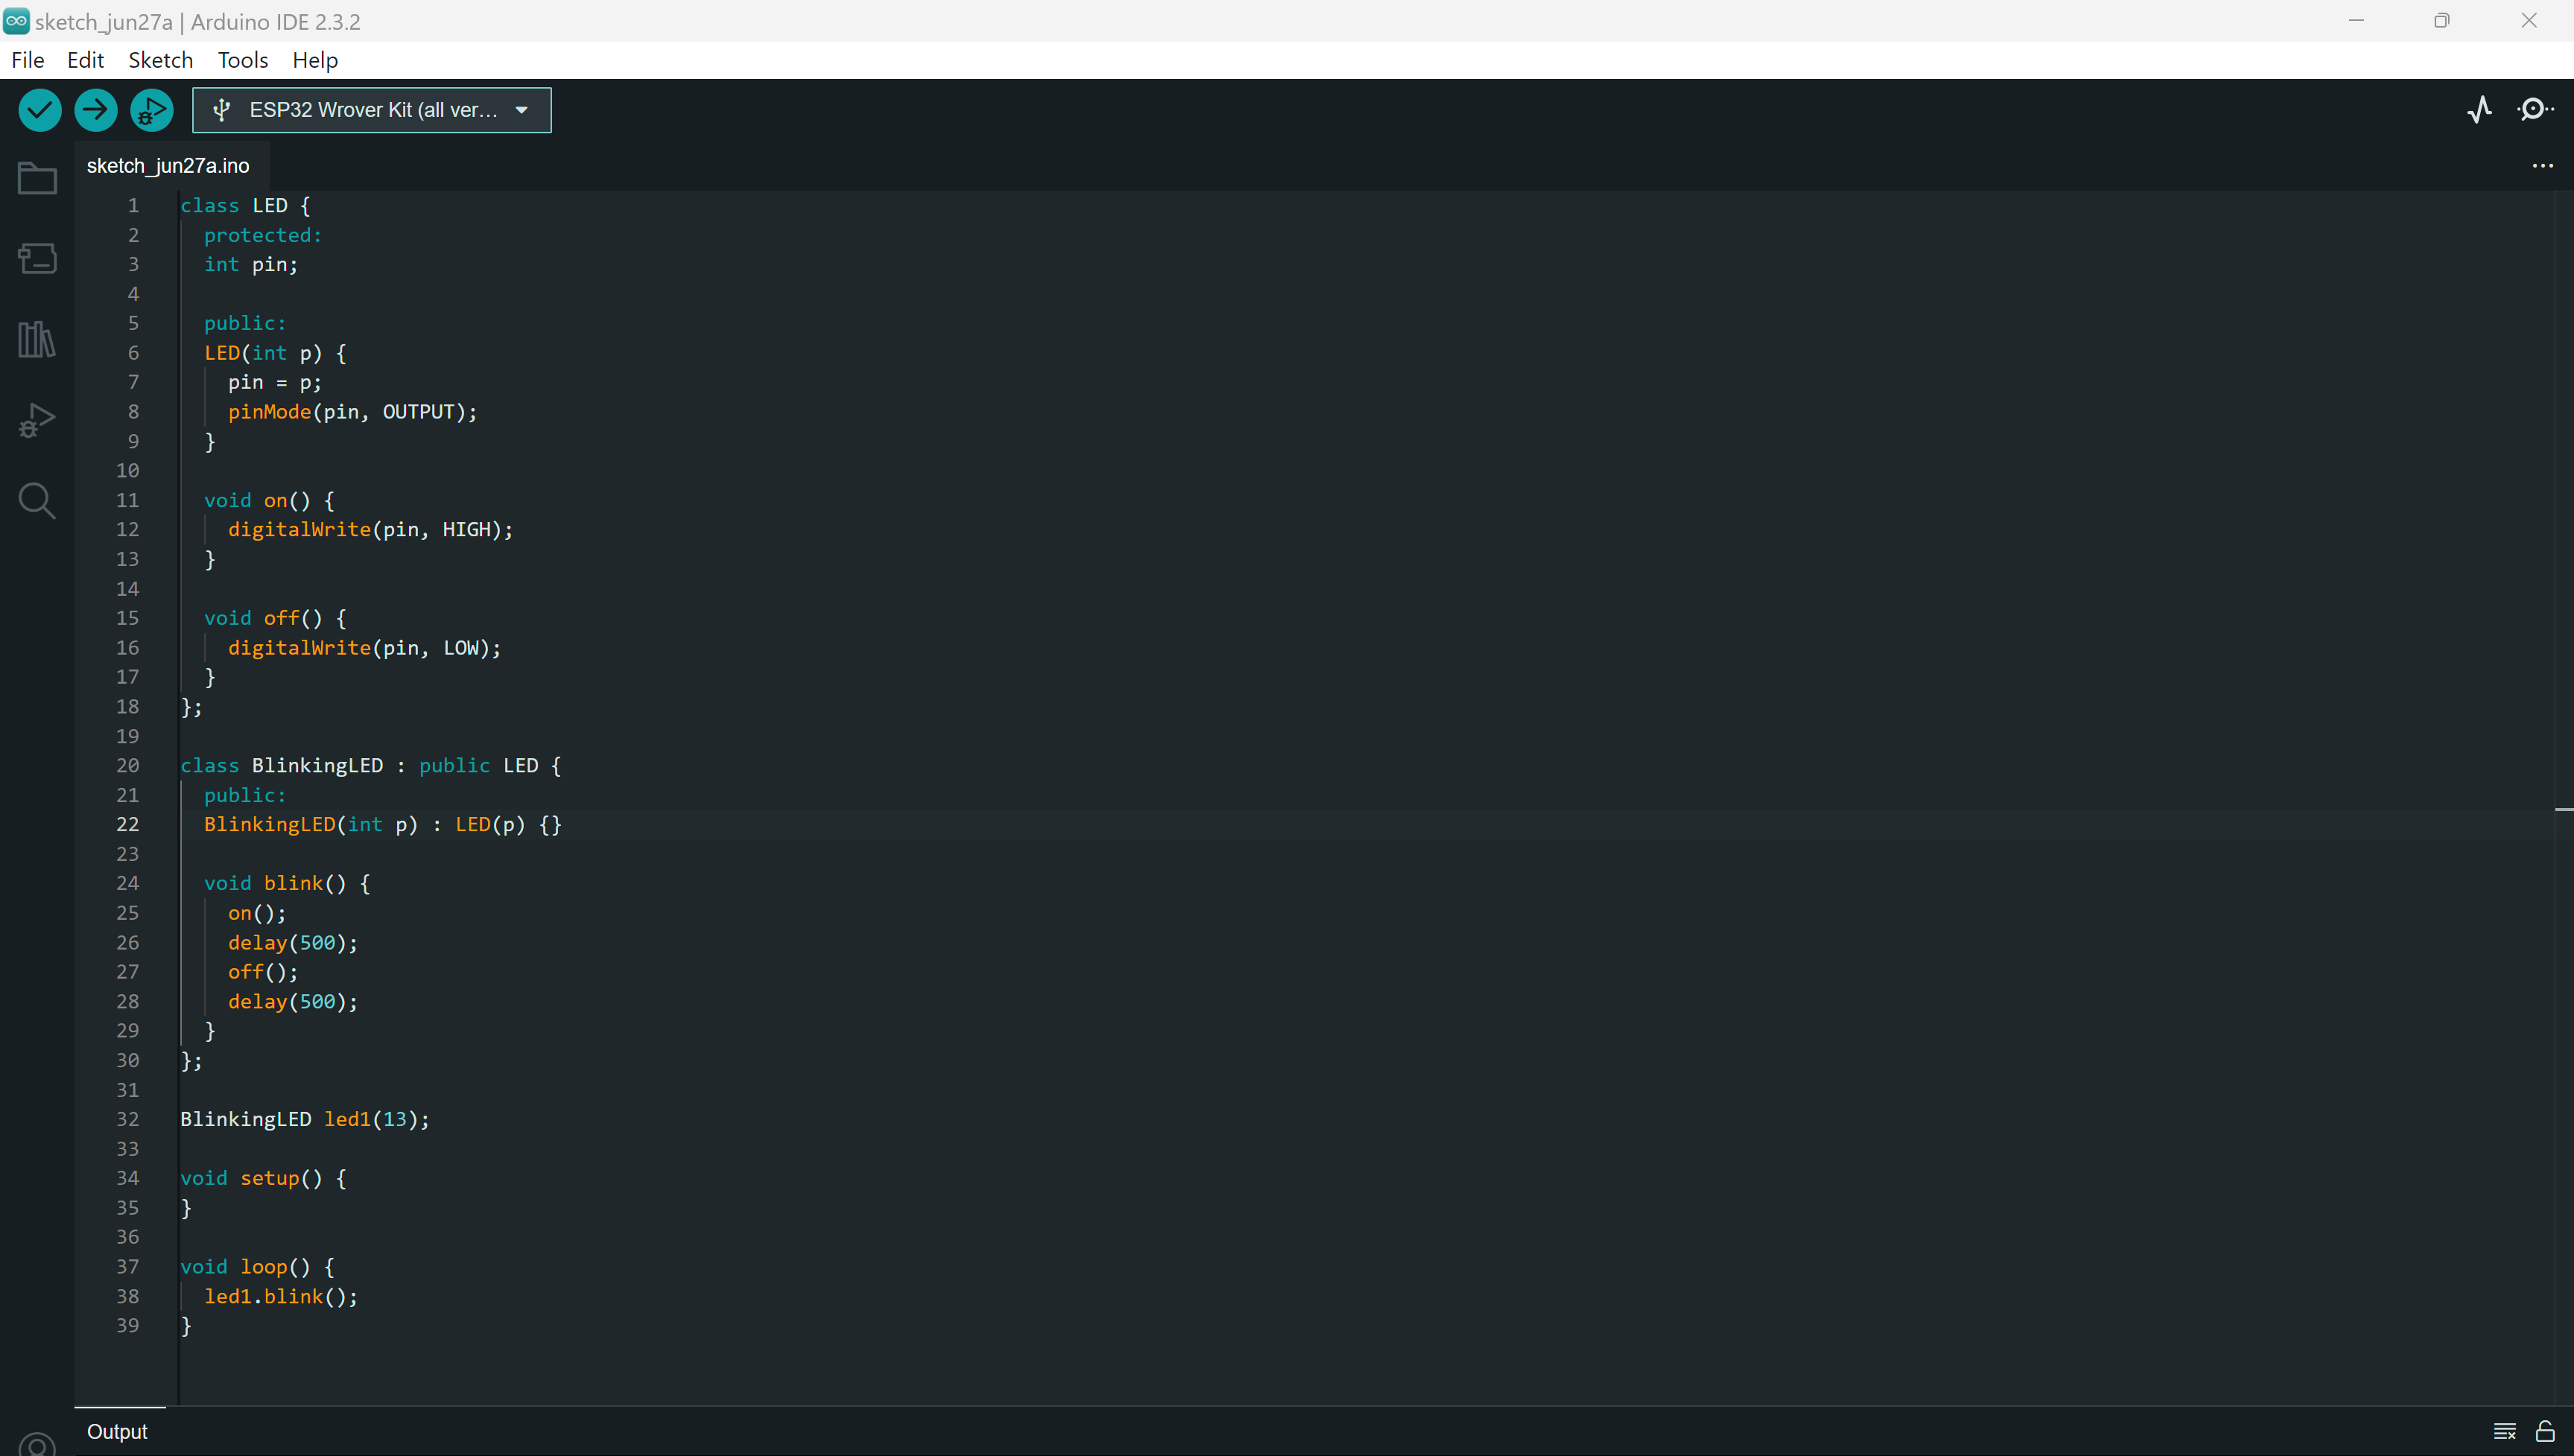
\includegraphics[width=\textwidth]{fig/fig14.png}
	\caption{C++ Inheritance}
	\label{fig:14}
\end{figure}

\subsection{C++ Polymorphism}
\textbf{Teori:} Polymorfisme tillader metoder at have forskellige implementeringer, selv når de deler samme navn. Dette opnås gennem virtual funktioner og arv. Virtual funktioner tillader afledte klasser at overskrive baseklassens funktioner, hvilket gør det muligt at kalde forskellige implementeringer afhængigt af objektets type.
\\\\
\noindent Polymorfisme gør det muligt at skrive fleksibel og udvidelig kode. Det tillader en funktion at håndtere objekter af forskellige typer på en ensartet måde, hvilket reducerer kompleksiteten og øger genanvendeligheden af koden.
\\\\
\noindent\textbf{Eksempel:}
\begin{lstlisting}[language=C++]
	class LED {
		protected:
		int pin;
		
		public:
		LED(int p) {
			pin = p;
			pinMode(pin, OUTPUT);
		}
		
		virtual void on() {
			digitalWrite(pin, HIGH);
		}
		
		virtual void off() {
			digitalWrite(pin, LOW);
		}
	};
	
	class BlinkingLED : public LED {
		public:
		BlinkingLED(int p) : LED(p) {}
		
		void on() override {
			digitalWrite(pin, HIGH);
			delay(500);
			digitalWrite(pin, LOW);
			delay(500);
		}
	};
	
	LED* led = new BlinkingLED(13);
	
	void setup() {
	}
	
	void loop() {
		led->on();
	}
\end{lstlisting}
\begin{figure}[h!]
	\centering
	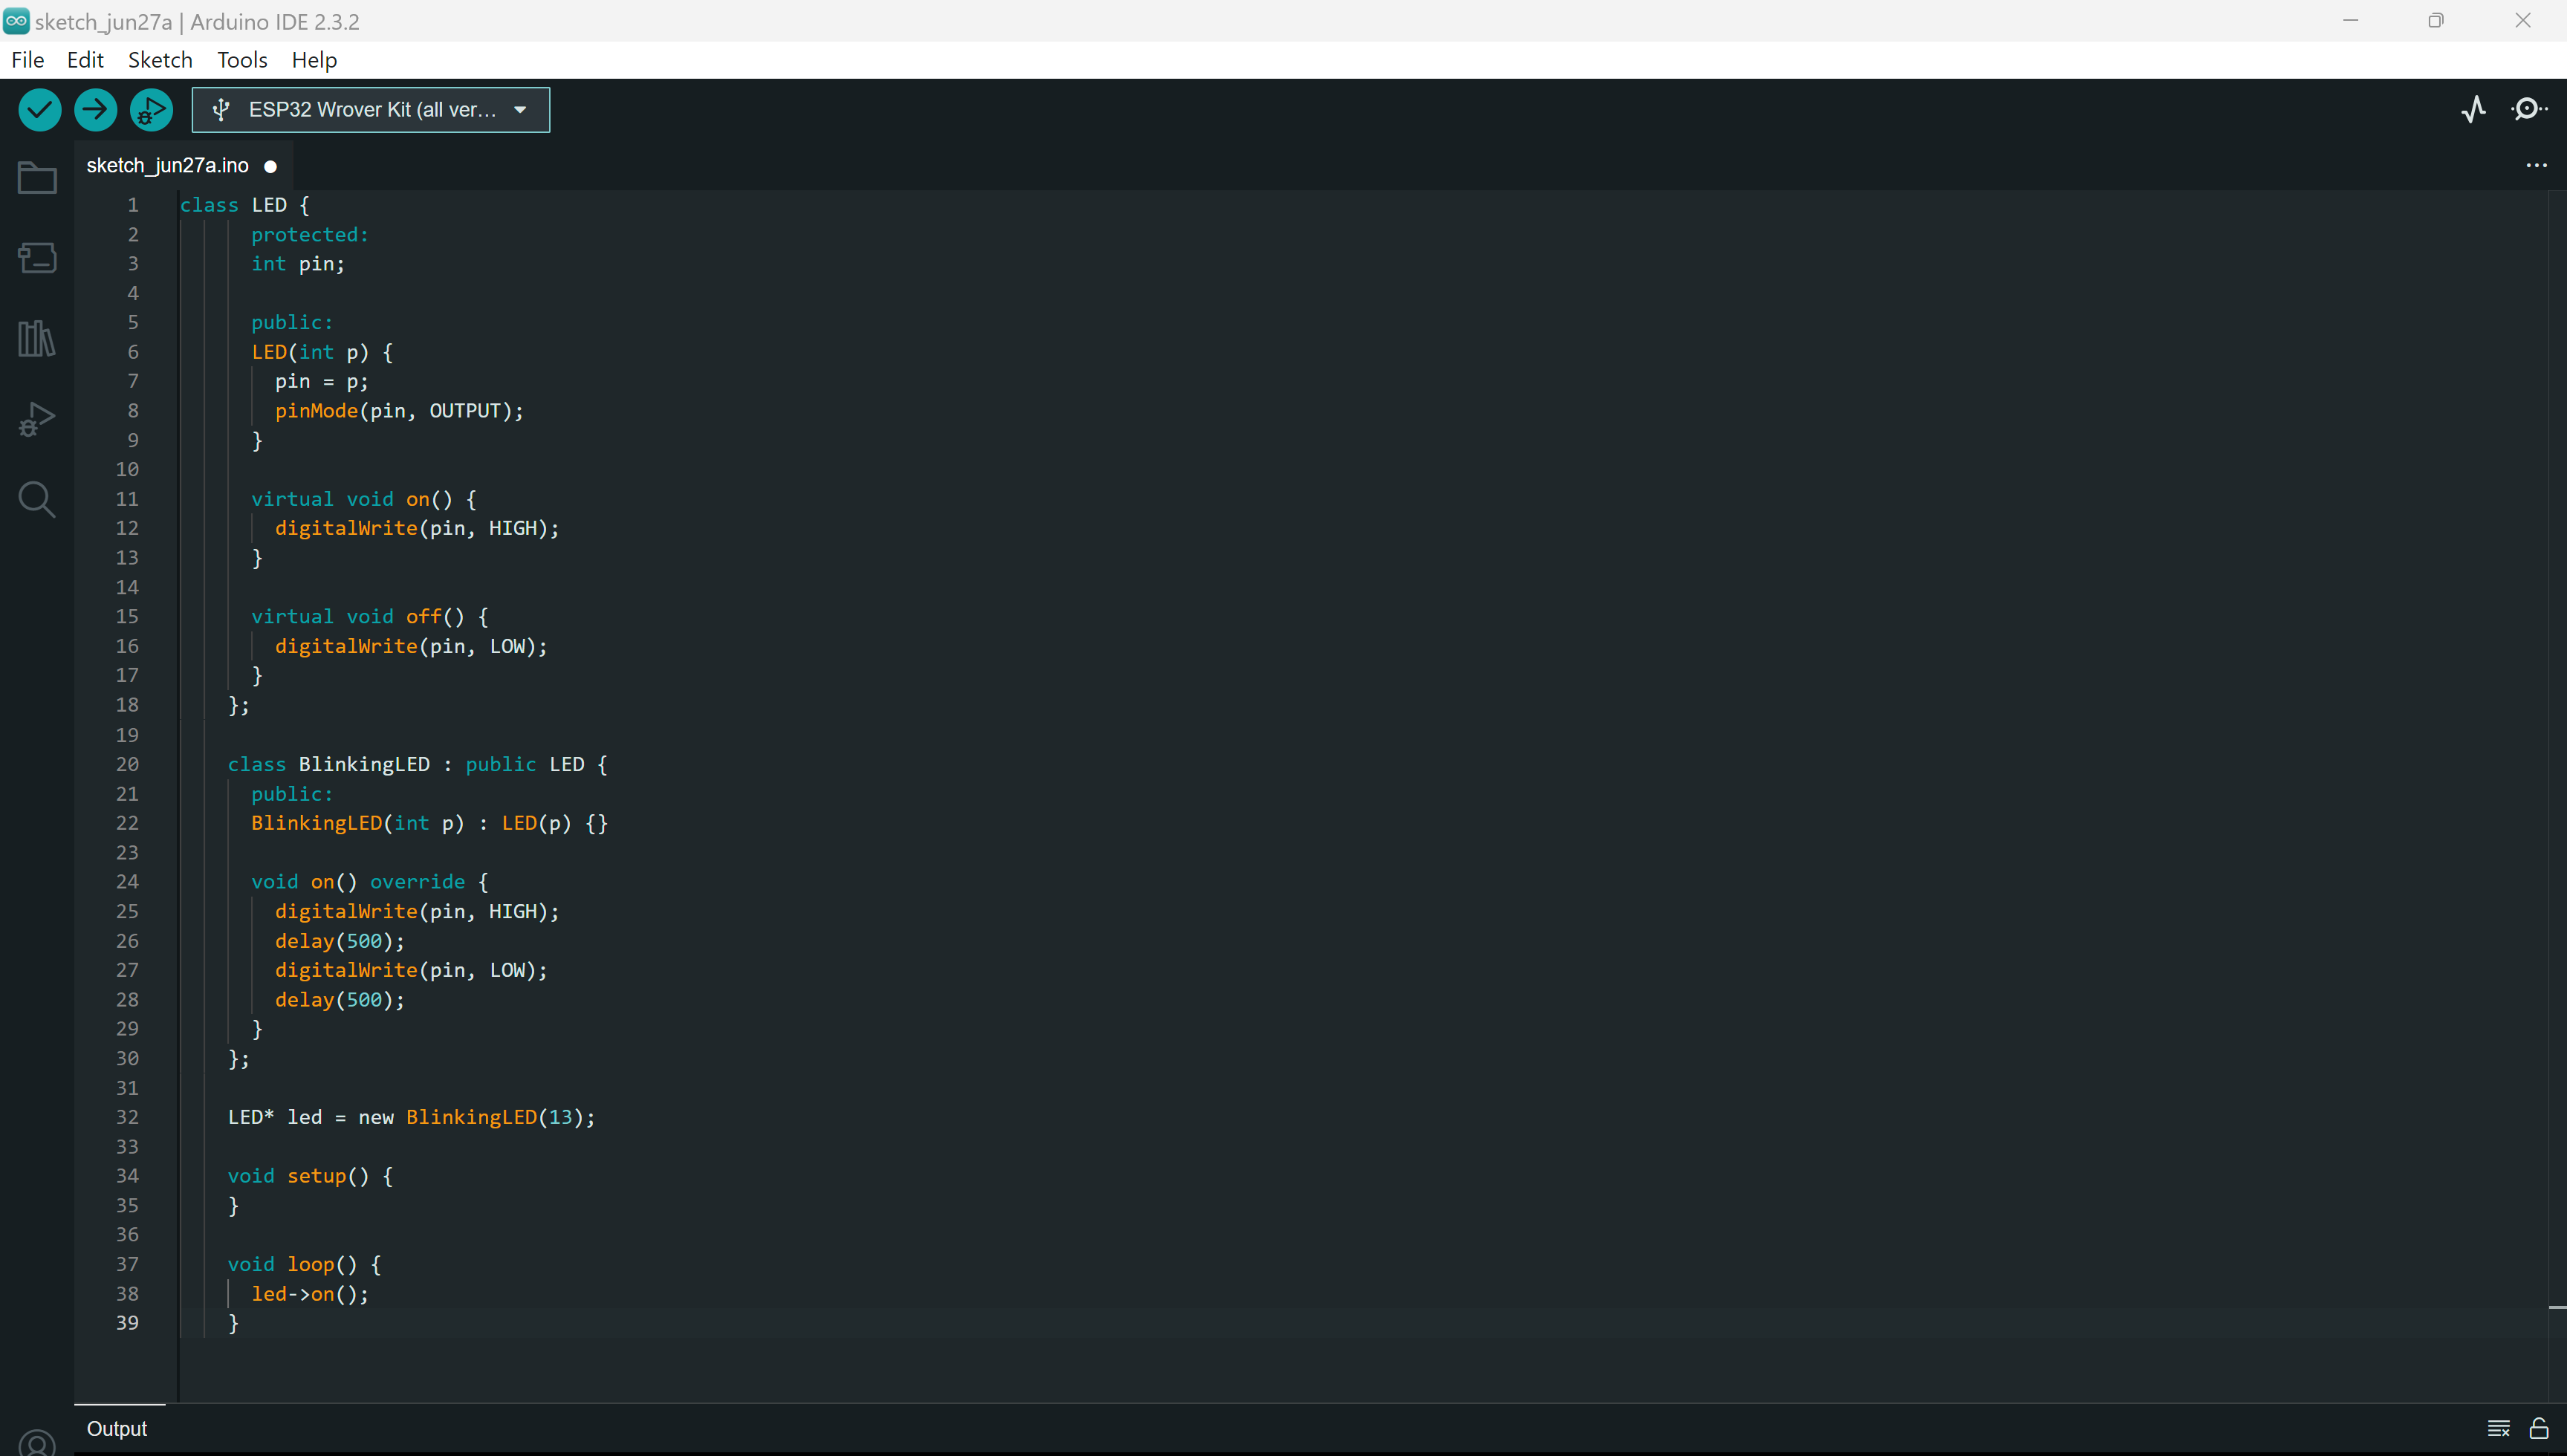
\includegraphics[width=\textwidth]{fig/fig20.png}
	\caption{text}
	\label{fig:20}
\end{figure}

\chapter{Opgave}
\textbf{Opgave:} Lav et Arduino-program, der bruger en klasse til at styre en LED. Klassen skal have metoder til at tænde, slukke og blinke LED'en. Brug en knap til at skifte mellem at tænde, slukke og blinke LED'en.
\begin{itemize}
	\item Opret en klasse \texttt{LED} med metoderne \texttt{on()}, \texttt{off()} og \texttt{blink()}.
	\item Brug en knap til at skifte mellem tilstande (tændt, slukket, blinkende).
	\item Brug \texttt{digitalRead()} til at læse knapstatus.
	\item Brug \texttt{digitalWrite()} til at styre LED'en.
\end{itemize}
\clearpage
\noindent\textbf{Løsningsforslag:}
\begin{lstlisting}[language=C++]
	class LED {
		int pin;
		
		public:
		// Constructor to initialize the LED pin
		LED(int p) {
			pin = p;
			pinMode(pin, OUTPUT);
		}
		
		// Turn the LED on
		void on() {
			digitalWrite(pin, HIGH);
		}
		
		// Turn the LED off
		void off() {
			digitalWrite(pin, LOW);
		}
		
		// Blink the LED with a 500ms delay (blocking function)
		void blink() {
			on();
			delay(500);
			off();
			delay(500);
		}
	};
	
	LED led(13);             // Create an LED object on pin 13
	int buttonPin = 2;       // Button input pin
	int buttonState = 0;     // Current state of the button
	int ledState = 0;        // 0: off, 1: on, 2: blink
	
	void setup() {
		pinMode(buttonPin, INPUT); // Initialize the button pin as input
	}
	
	void loop() {
		buttonState = digitalRead(buttonPin); // Read the button state
		
		// Check if the button is pressed
		if (buttonState == HIGH) {
			ledState = (ledState + 1) % 3; // Cycle through LED states
			delay(200); // Debounce delay (consider reducing to ~50-100ms)
		}
		
		// Handle the LED state
		switch (ledState) {
			case 0:
			led.off(); // Turn off the LED
			break;
			case 1:
			led.on();  // Turn on the LED
			break;
			case 2:
			led.blink(); // Blink the LED
			break;
		}
	}
\end{lstlisting}

%	Netværk basic
	\include{netværkbasic.tex}
%	IoT platform
	\part{IoT platform}
\chapter{Node-RED}
\section{Node-RED: En Teknisk Gennemgang}
\subsection{Introduktion til Node-RED}
Node-RED er et kraftfuldt udviklingsværktøj baseret på flow-baseret programmering, primært anvendt til at forbinde hardwareenheder, API'er og online-tjenester på nye og innovative måder. Det blev udviklet af IBM og er bygget på Node.js, hvilket gør det platform-uafhængigt, skalerbart og velegnet til IoT (Internet of Things) applikationer. Node-RED leverer en webbaseret editor, der gør det muligt for brugere at oprette JavaScript-funktioner og forbinde noder for at skabe flows. Disse flows kan interagere med forskellige protokoller og hardware, hvilket gør Node-RED til et alsidigt værktøj til IoT og automatiseringsopgaver. 

\begin{figure}[h!]
	\centering
	
\includegraphics[width=0.7\textwidth]{fig/fig26.png} % A high-level architecture diagram of Node-RED
	\caption{Node-RED}
\end{figure}

\subsection{Arkitektur og Kernekomponenter}
Node-RED's arkitektur er modulær og består af tre primære komponenter:

\subsubsection{Node-RED Runtime}
Runtime-miljøet er bygget på Node.js og er ansvarligt for at eksekvere flows, håndtere noder og håndtere meddelelser mellem noder. Det opererer inden for en enkelt-trådet event loop, typisk for Node.js-applikationer, hvilket muliggør asynkron behandling og non-blocking operationer. Runtime-miljøet indlæser flow-definitioner fra en JSON-fil og administrerer eksekveringen af noder, når meddelelser passerer gennem flowet. Det giver også API'er til at oprette, slette og administrere flows programmatisk.

\subsubsection{Node-RED Editor}
Node-RED editoren er en webbaseret grænseflade, der bruges til at udvikle flows. Den tilbyder en drag-and-drop grænseflade, hvor brugere kan placere noder på en arbejdsflade og forbinde dem for at definere dataflowet.

\begin{figure}[h!]
	\centering
	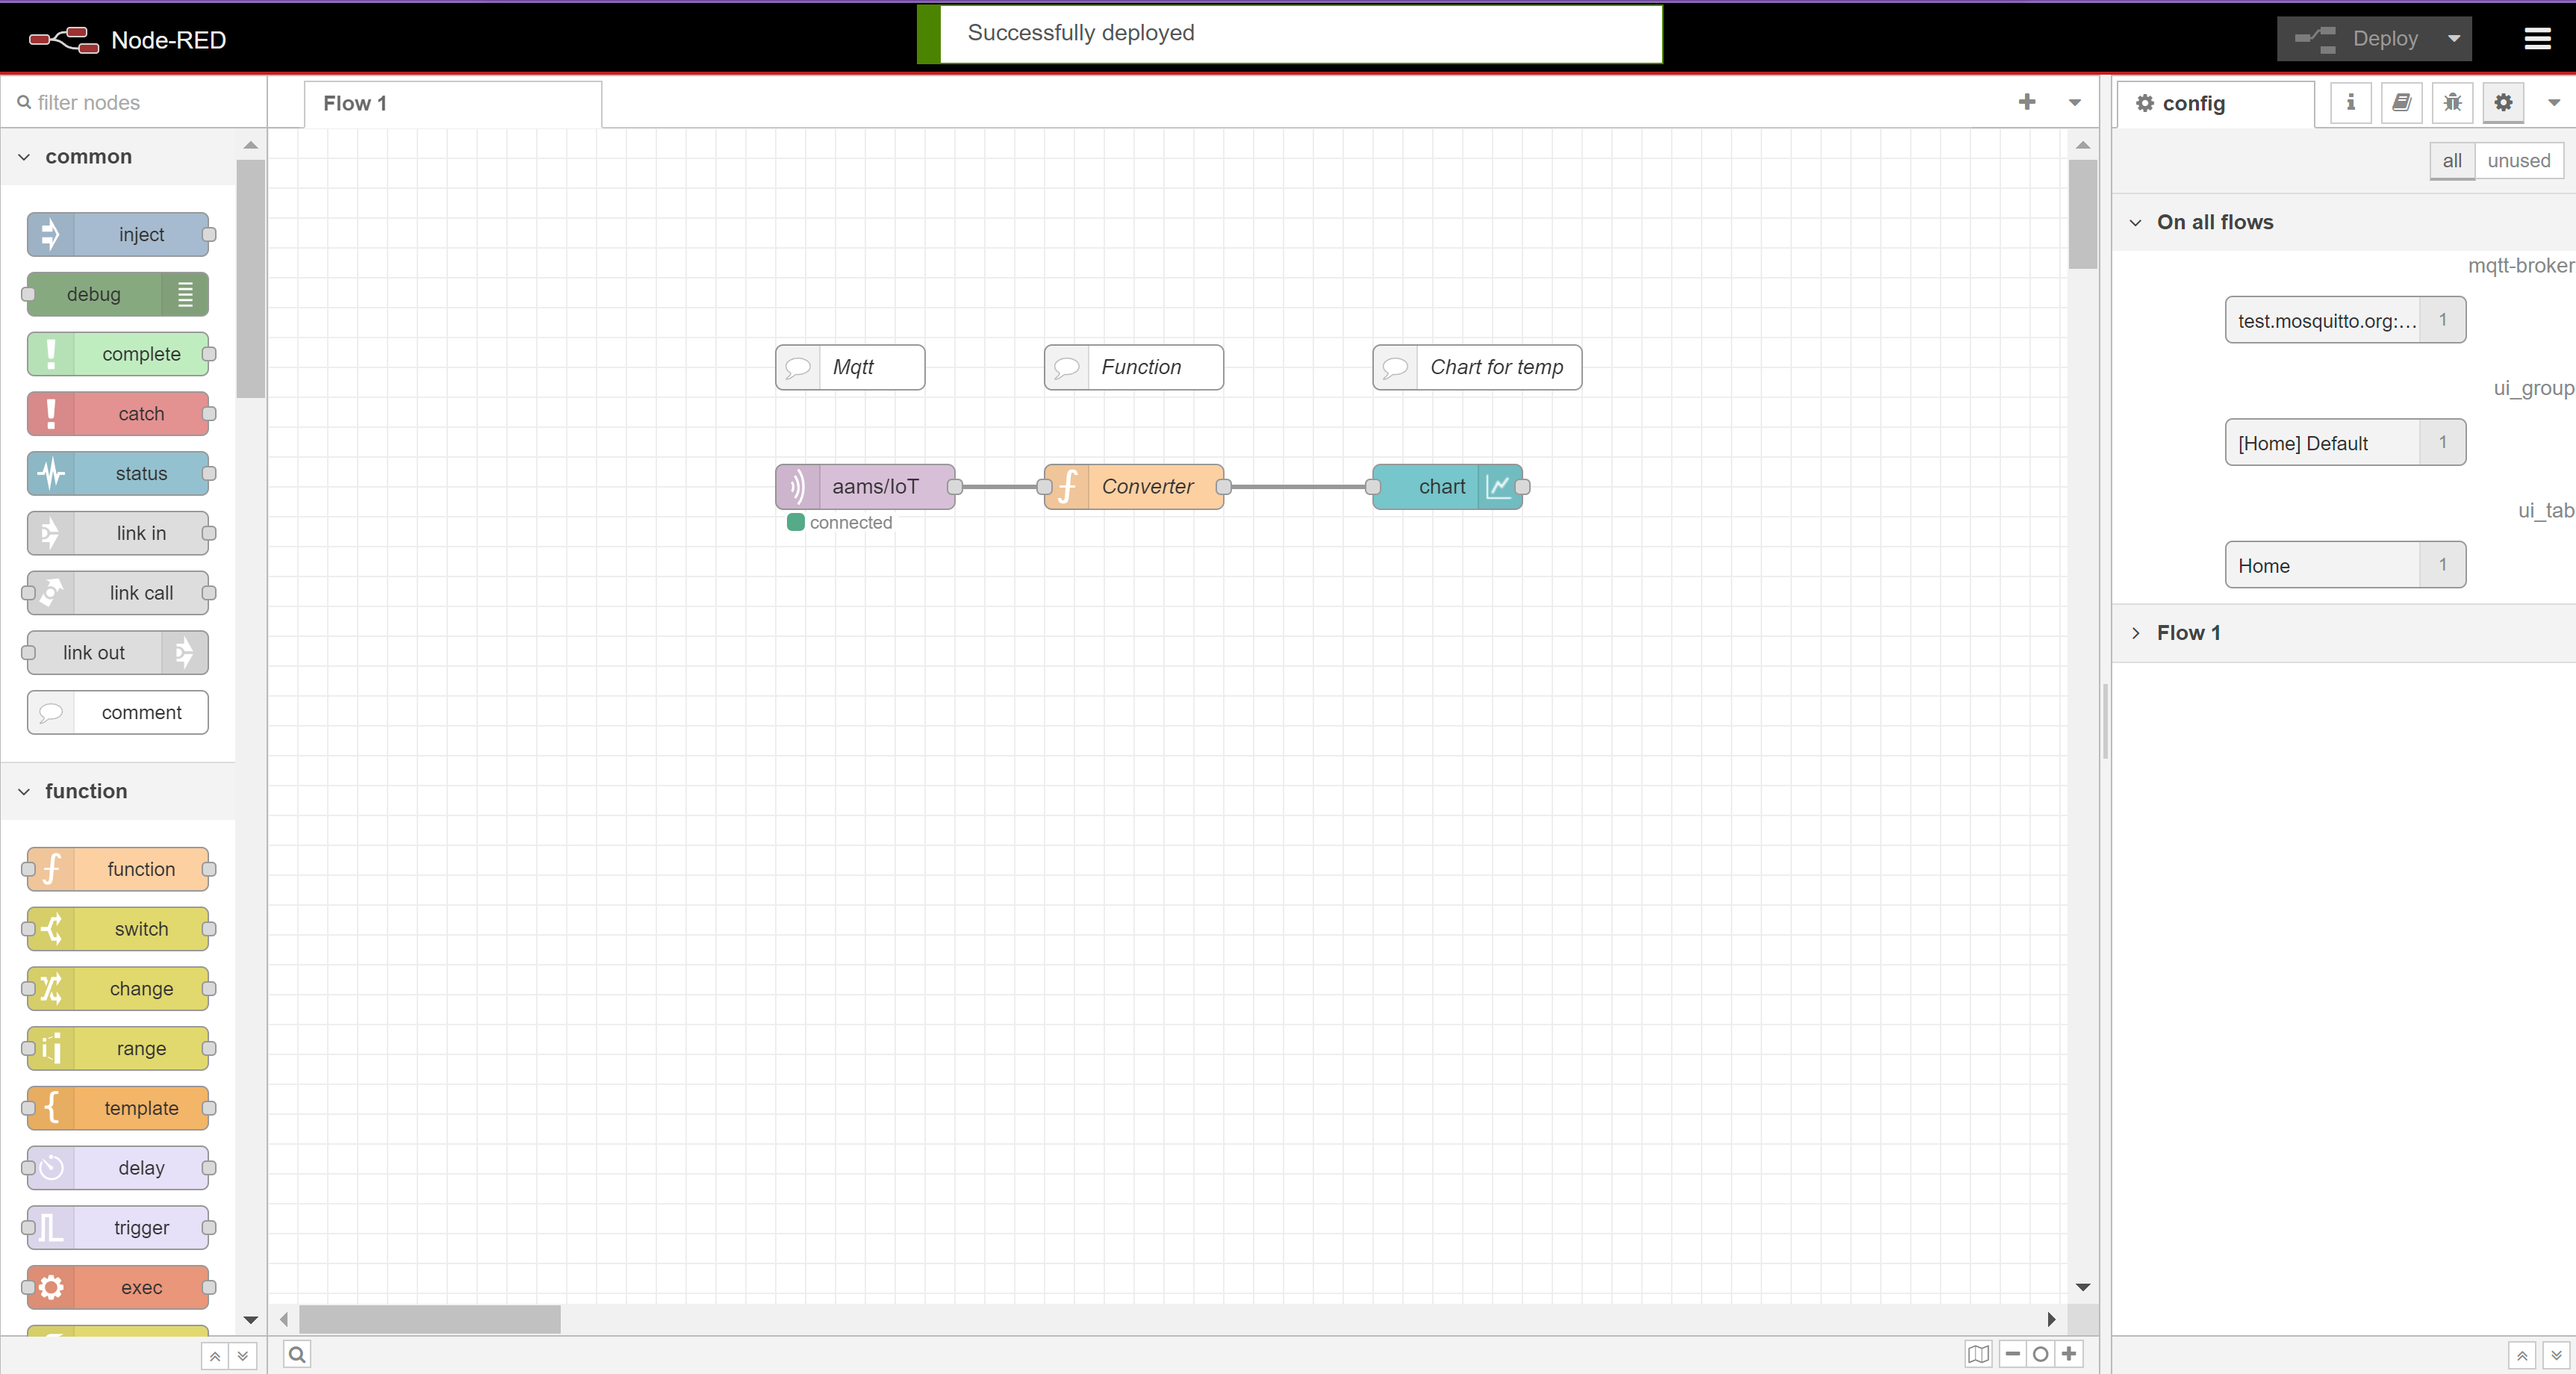
\includegraphics[width=\textwidth]{fig/fig25.png} % A screenshot of the Node-RED web-based editor with a simple flow
	\caption{Node-RED editoren med et simpelt flow, hvor noder er trukket ind i arbejdsområdet og forbundet.}
\end{figure}
\noindent Editorens kommunikation med runtime-miljøet sker via WebSocket og HTTP-protokoller, hvilket muliggør realtidsopdateringer og interaktion med kørende flows. Editorens output er JSON-baserede flow-definitioner, som derefter eksekveres af runtime-miljøet.

\subsubsection{Noder}
Noder er de grundlæggende byggeklodser i Node-RED. Hver node repræsenterer en specifik funktion, input, output eller serviceintegration. Noder kategoriseres i kerne-noder (som er indbygget i Node-RED) og bidrags-noder (som er tilgængelige via Node-RED-biblioteket). Noder kommunikerer ved at sende meddelelser til hinanden. Disse meddelelser er JavaScript-objekter, der kan indeholde data, konfigurationsindstillinger og metadata. Noder kan ændre, dirigere eller oprette meddelelser, mens de eksekverer.

\subsection{Flow-baseret Programmeringsparadigme}
Node-RED anvender et flow-baseret programmeringsparadigme, hvor udviklere opbygger applikationer ved at skabe flows eller grafer af noder, der repræsenterer behandlingsskridt. Hver node i et flow udfører en specifik opgave, såsom at læse sensordata, behandle dem og sende resultaterne til en database eller en ekstern API.

\subsubsection{Meddelelsesflow}
I Node-RED flyder meddelelser mellem noder langs definerede stier. Hver node behandler indkommende meddelelser og bestemmer, hvordan de skal ændres eller dirigeres til efterfølgende noder.

\subsubsection{Funktionsnoder}
For brugerdefineret logik tilbyder Node-RED funktionsnoder, hvor udviklere kan skrive JavaScript-kode. Dette muliggør kompleks databehandling, transformation og kontrollogik inden for et flow.

\subsection{Implementering og Skalerbarhed}
Node-RED er designet til at køre på en bred vifte af platforme, fra små enheder som Raspberry Pi til cloud-baserede tjenester. Implementering kan være så simpelt som at køre en lokal instans på en enkelt maskine eller at implementere i et cloud-miljø ved hjælp af Docker eller andre containerteknologier.

\subsubsection{Skalerbarhed}
Node-RED's event-drevne, non-blocking arkitektur gør det iboende skalerbart. Det kan håndtere flere forbindelser og høj-throughput datastreams, hvilket gør det velegnet til store IoT-implementeringer.

\subsubsection{Clustering}
Selvom Node-RED ikke selv understøtter clustering, kan det implementeres i et klynge-miljø ved hjælp af værktøjer som Kubernetes, hvilket muliggør skalering på tværs af flere noder og fejltolerance.

\subsection{Integration med IoT Protokoller og Tjenester}
Node-RED er særligt kraftfuldt inden for IoT på grund af dets omfattende understøttelse af forskellige protokoller og tjenester:

\subsubsection{MQTT}
Node-RED understøtter naturligt MQTT (Message Queuing Telemetry Transport), en letvægtsbeskedsprotokol, der ofte anvendes i IoT. MQTT-noder kan bruges til at abonnere på emner, publicere meddelelser og integrere med MQTT-brokers.

\subsubsection{HTTP og WebSocket}
Node-RED tilbyder noder til håndtering af HTTP og WebSocket-kommunikation, hvilket muliggør integration med webtjenester, RESTful API'er og realtidsapplikationer.

\subsubsection{Modbus, OPC-UA og Andre Industrielle Protokoller}
Til industrielle IoT-applikationer (IIoT) tilbyder Node-RED noder til interaktion med Modbus, OPC-UA og andre industrielle protokoller. Dette muliggør interface med PLC'er, SCADA-systemer og andet industrielt udstyr.

\subsubsection{Cloud Tjenester}
Node-RED kan integrere med cloud-tjenester såsom AWS, Azure og Google Cloud, hvilket tillader data at blive sendt til cloud-databaser, behandlet af cloud-funktioner eller visualiseret ved hjælp af cloud-dashboards.

\subsection{Sikkerhed og Godkendelse}
Sikkerhed er et kritisk aspekt af enhver IoT-implementering, og Node-RED tilbyder flere mekanismer til at sikre sikker drift:

\subsubsection{Brugergodkendelse}
Node-RED kan konfigureres til at kræve brugergodkendelse for adgang til editoren og API'er. Dette gøres typisk ved hjælp af HTTP basic authentication eller ved integration med eksterne godkendelsesudbydere.

\subsubsection{TLS/SSL}
Node-RED understøtter TLS/SSL-kryptering for at sikre HTTP, WebSocket og MQTT-kommunikation. Dette sikrer, at data, der sendes til og fra Node-RED, er beskyttet mod aflytning og manipulation.

\subsection{Udvidelsesmuligheder og Custom Noder}
Node-RED er designet til at være fleksibelt og udvidelsesbart. Ud over de mange indbyggede noder kan udviklere oprette og dele deres egne custom noder.

\subsubsection{Oprettelse af Custom Noder}
Udviklere kan oprette custom noder ved hjælp af JavaScript og Node.js-økosystemet. Disse noder kan derefter integreres i Node-RED editoren og bruges sammen med eksisterende noder.

\chapter{Opgaver}
\section{Modtagelse af Seriel Data fra ESP32 i Node-RED}
I denne sektion beskrives processen for, hvordan man kan opsætte og modtage seriel data fra en ESP32-mikrocontroller til Node-RED. Seriel kommunikation er en simpel og effektiv måde at overføre data mellem enheder, og ved at integrere dette med Node-RED, kan dataene nemt visualiseres, behandles eller videresendes.

\subsection{Opsætning af Seriel Kommunikation}
For at opsætte seriel kommunikation mellem ESP32 og Node-RED skal følgende trin følges:

\begin{enumerate}
	\item \textbf{Forbind ESP32 til Computeren:} Start med at forbinde din ESP32 til din computer via USB. Dette vil oprette en seriel forbindelse, som både ESP32 og Node-RED kan kommunikere over.
	
	\item \textbf{Installér Serial Node i Node-RED:} Åbn Node-RED og installér \texttt{node-red-node-serialport}, hvis det ikke allerede er installeret. Dette bibliotek giver adgang til at læse og skrive seriel data i Node-RED.
	
	\item \textbf{Tilføj og Konfigurer en Serial In Node:} Træk en \texttt{serial in} node ind i dit flow i Node-RED. Konfigurer noden til at lytte på den serielle port, som din ESP32 er tilsluttet. Sørg for, at baudraten og andre kommunikationsparametre matcher dem, der er indstillet på ESP32.
	
	\item \textbf{Tilføj en Debug Node:} For at kunne se de data, som modtages via den serielle port, tilføj en \texttt{debug} node og forbind den til \texttt{serial in} noden. Dette vil vise de modtagne data i Node-RED's debug-vindue.
	
	\item \textbf{Programmering af ESP32:} Upload en simpel skitse til din ESP32, der sender data via seriel kommunikation. Dette kan være så simpelt som at sende en tekststreng eller sensordata hver gang en bestemt hændelse indtræffer.
	
	\item \textbf{Kør Flowet i Node-RED:} Når alle trin er fulgt, kan du køre dit flow i Node-RED. Data, der sendes fra ESP32, vil nu kunne ses i debug-vinduet i Node-RED.
	
\end{enumerate}
Denne proces sikrer, at data fra din ESP32 kan modtages og håndteres i Node-RED, hvilket gør det muligt at integrere enheder og sensorer i dit IoT-netværk.

\subsection{Opgave: Modtagelse og Visualisering af Temperaturdata fra ESP32 i Node-RED}
\noindent \textbf{Mål:} Konfigurer Node-RED til at modtage seriel data fra en ESP32, som sender temperaturmålinger, og visualiser dataene i Node-RED's dashboard.

\subsubsection*{Opgavebeskrivelse:}
\begin{enumerate}
	\item \textbf{Forberedelse:}
	\begin{itemize}
		\item Installer \texttt{node-red-node-serialport} i Node-RED.
		\item Sørg for, at din ESP32 er forbundet til din computer via USB.
		\item Upload en skitse til ESP32, der måler temperaturen (f.eks. med en DHT11-sensor) og sender dataene via den serielle port.
	\end{itemize}
	
	\item \textbf{Implementering:}
	\begin{itemize}
		\item Tilføj en \texttt{serial in} node i Node-RED og konfigurer den til at læse data fra den korrekte serielle port.
		\item Tilføj en \texttt{debug} node for at sikre, at dataene modtages korrekt.
		\item Tilføj en \texttt{chart} node i Node-RED's dashboard for at visualisere temperaturdataene.
		\item Forbind noderne i Node-RED, så dataene flyder fra \texttt{serial in} noden til \texttt{chart} noden via en funktion eller \texttt{change} node for at formatere dataene korrekt.
	\end{itemize}
	
	\item \textbf{Test:}
	\begin{itemize}
		\item Start flowet i Node-RED og verificer, at temperaturdataene modtages korrekt og vises i dashboardet.
		\item Juster om nødvendigt dataformatet eller baudraten for at sikre, at al kommunikation sker uden fejl.
	\end{itemize}
\end{enumerate}
\noindent \textbf{Formål:} Formålet med denne opgave er at lære at opsætte seriel kommunikation mellem en ESP32 og Node-RED, samt hvordan man kan visualisere sensor data i et brugervenligt dashboard.
	
%	\part{Protokoller}
%	
\chapter{TCP/IP}
\section{TCP-protokollen}
\subsubsection*{Introduktion til TCP i Embedded Systems}
TCP (Transmission Control Protocol) er en forbindelsesorienteret protokol, der bruges til pålidelig dataoverførsel mellem enheder på et netværk. I modsætning til UDP sikrer TCP, at alle datapakker ankommer i den rigtige rækkefølge og uden tab. Dette gør TCP velegnet til applikationer, hvor dataens integritet og rækkefølge er afgørende, såsom i filoverførsler eller kommunikation med databaser.

\subsubsection*{TCP's Funktionsmåde}
\paragraph{Trevejs-håndtrykket (Three-Way Handshake)}
TCP-forbindelsen etableres gennem en proces kaldet trevejs-håndtrykket. Denne proces sikrer, at både klienten og serveren er synkroniseret og klar til at kommunikere. Processen involverer tre trin:
\begin{enumerate}
	\item \textbf{SYN (Synchronize):} Klienten sender en SYN-pakke til serveren for at anmode om at oprette en forbindelse.
	\item \textbf{SYN-ACK (Synchronize-Acknowledge):} Serveren svarer med en SYN-ACK-pakke, der bekræfter modtagelsen af SYN-pakken og anmoder om at oprette forbindelse til klienten.
	\item \textbf{ACK (Acknowledge):} Klienten sender en ACK-pakke for at bekræfte modtagelsen af serverens SYN-ACK-pakke. Efter dette trin er forbindelsen etableret.
\end{enumerate}
Dette trevejs-håndtryk er en grundlæggende del af TCP, der sikrer pålidelighed i forbindelsen.

\begin{figure}[!h]
	\centering
	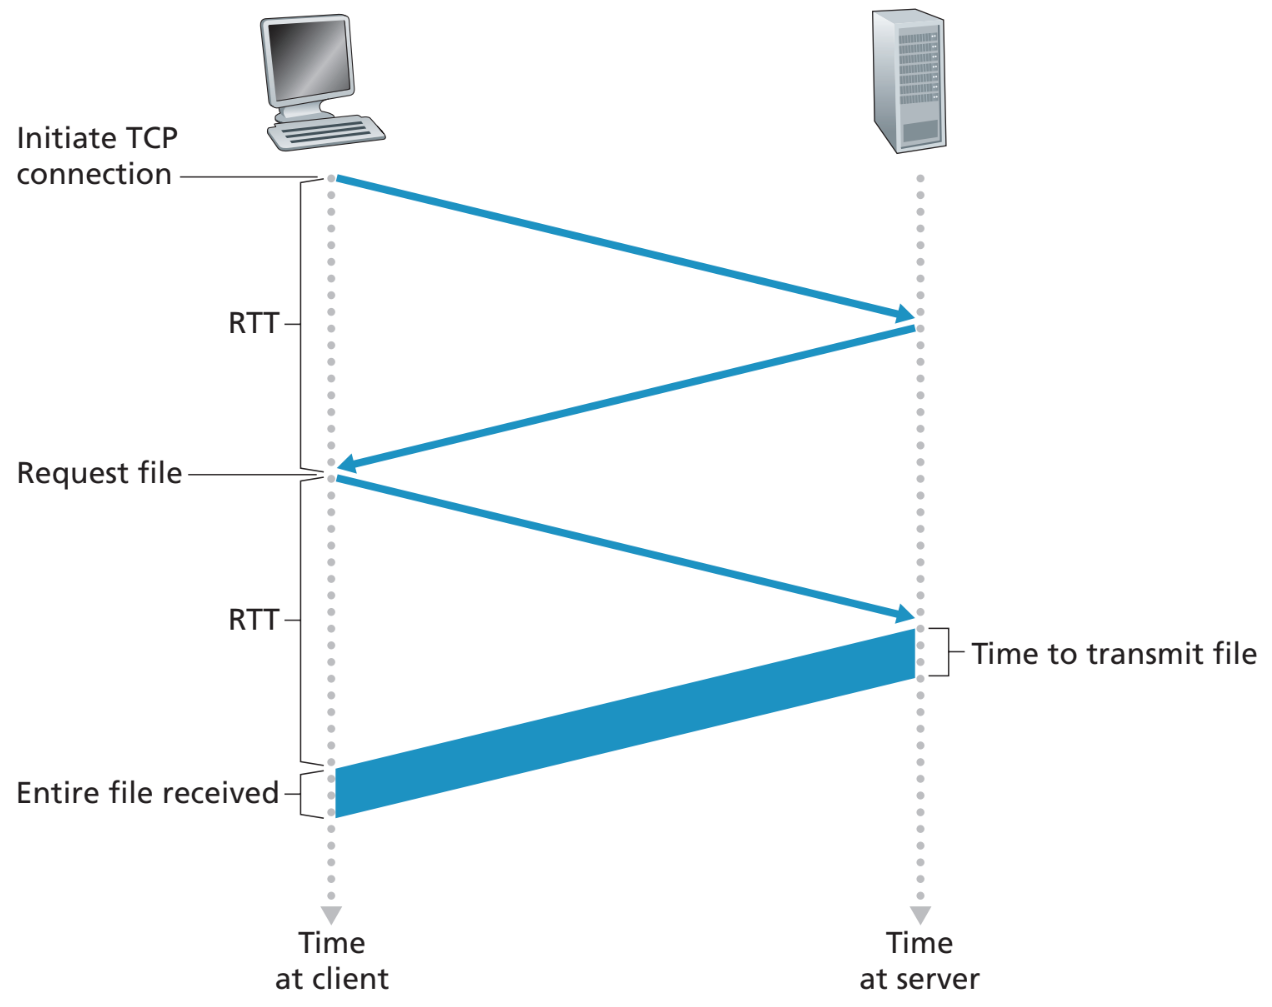
\includegraphics{fig/fig27.png}
	\caption{Three-way handshake}
\end{figure}

\paragraph{Dataoverførsel og Fejlhåndtering}
Når forbindelsen er etableret, opdeler TCP de data, der skal sendes, i segmenter. Hvert segment sendes separat og bekræftes af modtageren ved hjælp af ACK-pakker. Hvis et segment går tabt eller modtages i en forkert rækkefølge, sørger TCP for at sende det igen, indtil modtageren bekræfter det. Dette sikrer, at alle data ankommer i den rigtige rækkefølge og uden tab.
\newline\newline\noindent
TCP bruger også en mekanisme kaldet "flow control" for at sikre, at modtageren ikke bliver overvældet af for mange data ad gangen. Dette gør TCP velegnet til applikationer, hvor stabil og ordnet dataoverførsel er nødvendig.

\paragraph{Brug af TCP i Embedded Systems}
I indlejrede systemer bruges TCP ofte til applikationer, hvor pålidelighed er afgørende, såsom i dataoverførsler mellem en IoT-enhed og en central server. For eksempel kan en sensor, der sender kritiske data til en cloud-server, bruge TCP for at sikre, at dataene ankommer uden fejl eller tab.

\paragraph{Sikkerhed i TCP}
For at beskytte data under overførsel kan TCP kombineres med TLS (Transport Layer Security), som giver kryptering og beskytter mod aflytning og manipulation. Dette er især vigtigt i applikationer, hvor følsomme data overføres over internettet.

\subsubsection{Integration af ESP32 med TCP}
I dette afsnit beskrives de nødvendige trin for at integrere ESP32 med TCP:

\begin{enumerate}
	\item \textbf{Inkluder nødvendige biblioteker}
	\begin{lstlisting}[language=C++, caption=Syntaks]
		#include <WiFi.h>       // WiFi library for ESP32
	\end{lstlisting}
	\noindent Denne linje inkluderer det nødvendige bibliotek for WiFi-forbindelse på ESP32.
	
	\item \textbf{Definer WiFi og TCP-oplysninger}
	\begin{lstlisting}[language=C++, caption=Syntaks]
		const char* ssid = "your_network_name";   // WiFi SSID
		const char* password = "your_password";   // WiFi password
		const char* serverAddress = "server_address"; // TCP server IP address
		const int serverPort = 8080;              // TCP server port
	\end{lstlisting}
	\noindent Her defineres netværksnavnet og adgangskoden til dit WiFi-netværk samt TCP-serverens IP-adresse og port.
	
	\item \textbf{Opret WiFi klient og TCP forbindelse}
	\begin{lstlisting}[language=C++, caption=Syntaks]
		WiFiClient client;  // Create WiFi client object
	\end{lstlisting}
	\noindent Dette skaber et klientobjekt til at styre TCP-forbindelsen.
	
	\item \textbf{Initialiser WiFi-forbindelsen i Setup}
	\begin{lstlisting}[language=C++, caption=Syntaks]
		void setup() {
			Serial.begin(115200); // Start serial communication
			WiFi.begin(ssid, password); // Connect to WiFi
			while (WiFi.status() != WL_CONNECTED) {
				delay(1000); // Wait until connected
				Serial.println("Connecting to WiFi...");
			}
			Serial.println("Connected to WiFi");
		}
	\end{lstlisting}
	\noindent I setup-funktionen initialiseres WiFi-forbindelsen.
	
	\item \textbf{Eksempel på TCP dataoverførsel i Loop}
	\begin{lstlisting}[language=C++, caption=Syntaks]
		void loop() {
			if (!client.connected()) {
				Serial.println("Connecting to server...");
				client.connect(serverAddress, serverPort); // Connect to TCP server
				Serial.println("Connected to server!");
			}
			
			// Send data to the server
			client.println("Hello, Server!");
			
			// Receive data from the server
			while (client.available()) {
				String line = client.readStringUntil('\r');
				Serial.print(line);
			}
			
			delay(10000); // Wait 10 seconds before the next update
		}
	\end{lstlisting}
	Dette eksempel viser, hvordan ESP32 kan sende en besked til en TCP-server og modtage et svar.
	
	\item \textbf{Eksempel på TCP-server på ESP32}
	\begin{lstlisting}[language=C++, caption=Syntaks]
		WiFiServer server(serverPort); // Create a TCP server object
		
		void setup() {
			Serial.begin(115200); // Start serial communication
			WiFi.begin(ssid, password); // Connect to WiFi
			while (WiFi.status() != WL_CONNECTED) {
				delay(1000); // Wait until connected
				Serial.println("Connecting to WiFi...");
			}
			Serial.println("Connected to WiFi");
			
			server.begin(); // Start the server
		}
		
		void loop() {
			WiFiClient client = server.available(); // Check if a client has connected
			if (client) {
				String request = client.readStringUntil('\r');
				Serial.println(request);
				client.flush();
				
				// Handle the client's request
				client.println("HTTP/1.1 200 OK");
				client.println();
				client.stop(); // Close the connection
			}
		}
	\end{lstlisting}
	Dette eksempel viser, hvordan ESP32 kan fungere som en TCP-server, modtage forbindelser fra klienter og sende svar.
\end{enumerate}
\noindent Denne procedure skitserer trin for trin, hvordan ESP32 kan integreres med TCP-protokollen for at kommunikere effektivt i et IoT-miljø. TCP er ideelt til brug i situationer, hvor pålidelig og ordnet dataoverførsel er nødvendig, såsom i applikationer, der kræver en høj grad af dataintegritet.


\chapter{UDP}
\section{UDP-protokollen}
\subsubsection*{Introduktion til UDP i Embedded Systems}
UDP (User Datagram Protocol) er en letvægts, forbindelsesløs kommunikationsprotokol, der anvendes på tværs af netværk til hurtig og effektiv dataoverførsel. I modsætning til TCP (Transmission Control Protocol) giver UDP ingen garantier for levering, rækkefølge eller beskyttelse mod duplikation, hvilket gør det hurtigere, men mindre pålideligt. Disse egenskaber gør UDP velegnet til applikationer, hvor hurtig dataoverførsel er vigtigere end pålidelighed, såsom i streaming eller sensor dataopsamling i indlejrede systemer.

\paragraph{Grundlæggende Funktionsmåde}
UDP fungerer ved at sende datagrammer, som er selvstændige pakker af data, til modtageren. Hver pakke behandles uafhængigt, og der er ingen håndtryk eller forbindelsesoprettelse mellem afsender og modtager, hvilket resulterer i minimal protokoloverhead og hurtigere kommunikation.

\paragraph{Unicast, Multicast og Broadcast}
UDP understøtter forskellige kommunikationstyper, herunder unicast, multicast og broadcast, som hver især er velegnet til forskellige typer af netværksapplikationer:

\begin{itemize}
	\item \textbf{Unicast:} I unicast kommunikation sendes data fra én afsender til én modtager. Dette er den mest almindelige form for kommunikation, hvor data leveres direkte til en specifik enhed.
	\item \textbf{Multicast:} Multicast tillader en enkelt afsender at sende data til flere udvalgte modtagere på én gang. Dette er effektivt i applikationer som streaming, hvor flere enheder skal modtage den samme information samtidig.
	\item \textbf{Broadcast:} I broadcast sendes data fra én afsender til alle enheder i et netværk. Dette bruges ofte i scenarier, hvor en besked skal nå alle tilgængelige enheder, som f.eks. i netværksopdagelse.
\end{itemize}

\paragraph{Fordele i Embedded Systems}
UDP's lette natur og hurtige\\ overførselshastighed gør det særligt velegnet til indlejrede systemer, hvor der kan være behov for at sende små mængder data hurtigt uden behov for bekræftelse. Dette gør det ideelt til real-time applikationer og enkle sensor-netværk.

\paragraph{Sikkerhed}
Da UDP ikke har indbyggede mekanismer til sikring af data, anbefales det at bruge UDP sammen med sikkerhedsprotokoller som DTLS (Datagram Transport Layer Security) for at beskytte data mod aflytning og manipulation.

\subsubsection{Integration af ESP32 med UDP}

Nedenstående kode viser, hvordan man integrerer ESP32 med UDP-protokollen. Koden omfatter opsætning af WiFi-forbindelse og både afsendelse og modtagelse af UDP-pakker.

\begin{lstlisting}[language=C++, caption=ESP32 integration med UDP]
	#include <WiFi.h>       // WiFi library for ESP32
	#include <WiFiUdp.h>    // UDP library for ESP32
	
	// WiFi og UDP konfigurationer
	const char* ssid = "your_network_name";   // WiFi SSID
	const char* password = "your_password";   // WiFi password
	const char* udp_server = "server_address"; // UDP server IP address
	const unsigned int udp_port = 12345;       // UDP server port
	
	WiFiUDP udpClient;  // Opret UDP klient objekt
	
	void setup() {
		Serial.begin(115200); // Start seriel kommunikation
		WiFi.begin(ssid, password); // Forbind til WiFi netværket
		while (WiFi.status() != WL_CONNECTED) {
			delay(1000); // Vent indtil forbindelsen er etableret
			Serial.println("Connecting to WiFi...");
		}
		Serial.println("Connected to WiFi");
	}
	
	void loop() {
		// Afsendelse af UDP pakke til serveren
		udpClient.beginPacket(udp_server, udp_port); // Start UDP pakke
		udpClient.print("Hello, UDP Server!"); // Tilføj besked til pakken
		udpClient.endPacket(); // Send UDP pakke
		
		delay(5000); // Vent 5 sekunder før næste pakke sendes
		
		// Modtagelse af UDP pakker fra serveren
		int packetSize = udpClient.parsePacket(); // Tjek for indkommende pakke
		if (packetSize) {
			char incomingPacket[255];
			int len = udpClient.read(incomingPacket, 255); // Læs pakken ind i buffer
			if (len > 0) {
				incomingPacket[len] = '\0'; // Null-terminer streng
			}
			Serial.print("Received UDP packet: ");
			Serial.println(incomingPacket); // Print modtaget pakke
		}
		
		delay(1000); // Vent 1 sekund før næste tjek
	}
\end{lstlisting}
Denne kode implementerer UDP-kommunikation på en ESP32-enhed. Den viser, hvordan man sender en simpel besked til en UDP-server og modtager data fra serveren. Ved at bruge WiFiUdp-biblioteket kan ESP32 kommunikere over UDP-protokollen, hvilket er ideelt til applikationer, der kræver hurtig og effektiv dataoverførsel, hvor levering af data ikke nødvendigvis skal bekræftes.




\chapter{Modbus}
\section{Modbus-protokollen}

\subsection{Introduktion til Modbus i Embedded Systems}
Modbus er en kommunikationsprotokol oprindeligt udviklet af Modicon (nu Schneider Electric) i slutningen af 1970'erne til brug i industrielt udstyr. Protokollen er blevet en industri-standard for kommunikation i industrielle systemer og er blevet adopteret bredt på grund af dens enkelhed og pålidelighed. Modbus anvendes ofte i indlejrede systemer, især hvor der er behov for kommunikation mellem mikrocontrollere, sensorer, aktuatorer og andre enheder over serielle forbindelser som RS-485 eller over TCP/IP.

\paragraph{Grundlæggende Funktionsmåde}
Modbus fungerer som en master/slave-protokol, hvor en master-enhed (f.eks. en PLC eller mikrocontroller) kommunikerer med en eller flere slave-enheder. Masteren initierer anmodninger, og slaverne reagerer på disse anmodninger. Modbus understøtter forskellige datatyper som coils, discrete inputs, input registers og holding registers, som kan bruges til at læse eller skrive data.

\paragraph{Modbus Function Codes}
Modbus-protokollen definerer forskellige funktionelle koder (function codes) for at udføre specifikke operationer. De mest almindelige funktioner inkluderer:
\begin{itemize}
	\item \textbf{01 - Read Coils}: Læser status af coils (0 eller 1), som er binære udgange, der kan tændes eller slukkes.
	\item \textbf{02 - Read Discrete Inputs}: Læser status af discrete inputs (0 eller 1), som er binære indgange.
	\item \textbf{03 - Read Holding Registers}: Læser værdien af holding registers, som normalt er brugt til at gemme outputdata.
	\item \textbf{04 - Read Input Registers}: Læser værdien af input registers, som normalt er brugt til at gemme inputdata.
	\item \textbf{05 - Write Single Coil}: Skriver en værdi til en enkelt coil.
	\item \textbf{06 - Write Single Register}: Skriver en værdi til et enkelt holding register.
	\item \textbf{15 - Write Multiple Coils}: Skriver værdier til flere coils.
	\item \textbf{16 - Write Multiple Registers}: Skriver værdier til flere holding registers.
\end{itemize}

\paragraph{Data Typer i Modbus}
Modbus definerer flere datatyper, som kan bruges til at interagere med enheder:
\begin{itemize}
	\item \textbf{Coils (0X)}: En coil er en binær output, som kan tændes (1) eller slukkes (0).
	\item \textbf{Discrete Inputs (1X)}: En discrete input er en binær input, som kan være høj (1) eller lav (0).
	\item \textbf{Input Registers (3X)}: Input registers er 16-bit værdier, der typisk bruges til at læse analoge inputdata.
	\item \textbf{Holding Registers (4X)}: Holding registers er 16-bit værdier, der typisk bruges til at gemme outputdata eller konfigurationer.
\end{itemize}

\paragraph{Fordele i Embedded Systems}
Modbus er meget effektiv i indlejrede systemer, hvor stabil kommunikation mellem enheder er nødvendig. Protokollen understøtter både seriel og TCP/IP kommunikation, hvilket gør den fleksibel til mange forskellige typer applikationer.

\paragraph{Sikkerhed}
Modbus i sin grundform tilbyder ikke nogen indbygget sikkerhed. For at sikre Modbus-kommunikation kan den dog køres over sikre transportlag som TLS, eller netværket kan sikres via VPN.

\subsubsection*{Integration af ESP32 med Modbus}
I dette afsnit beskrives de nødvendige trin for at integrere ESP32 med Modbus:

\begin{lstlisting}[language=C++, caption=Integration af ESP32 med Modbus]
	#include <WiFi.h>        // WiFi library for ESP32
	#include <ModbusIP_ESP8266.h> // Modbus TCP library for ESP32
	
	// WiFi configurations
	const char* ssid = "your_network_name";   // WiFi SSID
	const char* password = "your_password";   // WiFi password
	
	// Create Modbus server object
	ModbusIP mb;
	
	void setup() {
		Serial.begin(115200); // Start serial communication
		WiFi.begin(ssid, password); // Connect to WiFi
		
		// Wait for WiFi connection
		while (WiFi.status() != WL_CONNECTED) {
			delay(1000); 
			Serial.println("Connecting to WiFi...");
		}
		Serial.println("Connected to WiFi");
		
		mb.server();  // Start Modbus TCP server
	}
	
	void loop() {
		mb.task();  // Process incoming Modbus requests
		
		// Example: Update a holding register at address 0x0001 with the value 1234
		mb.Hreg(0x0001, 1234);
		
		delay(1000);  // Delay before the next operation
	}
\end{lstlisting}
Denne kode integrerer ESP32 med Modbus-protokollen og samler alle nødvendige funktioner, herunder WiFi-forbindelse, samt læsning og skrivning af coils og registre via Modbus, i én enkelt kodeblok. Dette sikrer robust og pålidelig kommunikation med Modbus-slaver, hvilket er afgørende i industrielle applikationer.	

\chapter{MQTT}
\section{MQTT-protokollen}
\subsubsection*{Introduktion til MQTT i Embedded Systems}
MQTT (Message Queue Telemetry Transport) er en letvægts, publikations- og abonnementsbaseret beskedprotokol, der er designet til at være effektiv og strømlinet, hvilket gør den ideel til brug i Embedded Systems. Dette gør den til en populær protokol indenfor IoT-området, hvor netværksbåndbredde og batteristrøm kan være begrænset.

\paragraph{Grundlæggende Funktionsmåde}
MQTT fungerer på en klient-server-model, hvor klienten kommunikerer med en mægler (broker). Klienter kan abonnere på emner (topics), og når en besked er offentliggjort på et emne af en anden klient, videresender mægleren beskeden til alle abonnenter på det pågældende emne.

\paragraph{QoS (Quality of Service)}
MQTT understøtter forskellige serviceniveauer, kaldet QoS. Disse niveauer bestemmer, hvordan og hvor ofte beskeder sendes:
\begin{itemize}
	\item \textbf{QoS 0}: "Højst én gang" - Beskeden sendes en enkelt gang uden bekræftelse.
	\item \textbf{QoS 1}: "Mindst én gang" - Beskeden sendes og bekræftes, men kan modtages mere end én gang.
	\item \textbf{QoS 2}: "Nøjagtigt én gang" - Beskeden sendes og bekræftes, så modtageren får den nøjagtigt én gang.
\end{itemize}

\paragraph{Fordel i Embedded Systems}
MQTT's letvægts natur og evne til at håndtere ustabile forbindelser gør den særligt velegnet til indlejrede systemer, hvor ressourcer kan være begrænsede. Derudover er dets publikations- og abonnementsmodel egnet til enheder, der kommunikerer over netværk med lav båndbredde.

\paragraph{Sikkerhed}
Selvom MQTT ikke i sig selv tilbyder avancerede sikkerhedsfunktioner, kan det kombineres med sikre transportlag som TLS for at tilbyde en sikker kommunikationskanal.

Dette afsnit giver en oversigt over MQTT og dens egenskaber, som gør den ideel til Embedded Systems. Det dækker grundlæggende funktioner, QoS-niveauer, fordelene ved brug i Embedded Systems og sikkerhedsaspekter.

\subsubsection{Integration af ESP32 med MQTT}

I dette afsnit beskrives de nødvendige trin for at integrere ESP32 med MQTT:

\begin{enumerate}
	\item \textbf{Inkluder nødvendige biblioteker}
	\begin{lstlisting}[language=C++, caption=Syntaks]
		#include <WiFi.h>
		#include <PubSubClient.h>
	\end{lstlisting}
	Disse linjer inkluderer de nødvendige biblioteker for WiFi-forbindelse og MQTT-klient.
	
	\item \textbf{Definer WiFi og MQTT-oplysninger}
	\begin{lstlisting}[language=C++, caption=Syntaks]
		const char* ssid = "your_network_name"; // WiFi SSID
		const char* password = "your_password"; // WiFi password
		const char* mqtt_server = "broker_address"; // MQTT broker address
	\end{lstlisting}
	Her defineres netværksnavnet og adgangskoden til dit WiFi-netværk samt MQTT-brokerens adresse.
	
	\item \textbf{Opret WiFiClient og PubSubClient}
	\begin{lstlisting}[language=C++, caption=Syntaks]
		WiFiClient espClient; // Create a WiFi client object
		PubSubClient client(espClient); // Create a PubSub client object
	\end{lstlisting}
	Dette skaber klientobjekter til at styre WiFi- og MQTT-forbindelserne.
	
	\item \textbf{Definer MQTT Reconnect-funktion}
	\begin{lstlisting}[language=C++, caption=Syntaks]
		void reconnect() {
			while (!client.connected()) {
				Serial.println("Connecting to MQTT..."); // Attempt to connect to MQTT broker
				if (client.connect("ESP32Client")) { // MQTT client ID
					Serial.println("Connected to MQTT!"); // Success message
				} else {
					delay(5000); // Wait before retrying
				}
			}
		}
	\end{lstlisting}
	Denne funktion forsøger at forbinde til MQTT-brokeren, indtil forbindelsen er etableret.
	
	\item \textbf{Initialiser WiFi-forbindelsen og MQTT i Setup}
	\begin{lstlisting}[language=C++, caption=Syntaks]
		void setup() {
			Serial.begin(115200); // Start serial communication
			WiFi.begin(ssid, password); // Connect to WiFi
			while (WiFi.status() != WL_CONNECTED) {
				delay(1000); // Wait until connected
				Serial.println("Connecting to WiFi...");
			}
			Serial.println("Connected to WiFi");
			client.setServer(mqtt_server, 1883); // Set MQTT broker and port
			reconnect(); // Connect to MQTT broker
		}
	\end{lstlisting}
	I setup-funktionen initialiseres forbindelsen til WiFi-netværket og MQTT-brokeren.
	
	\item \textbf{Publiser og abonner på emner i Loop}
	\begin{lstlisting}[language=C++, caption=Syntaks]
		void loop() {
			if (!client.connected()) {
				reconnect(); // Ensure connection to MQTT broker
			}
			client.loop(); // Maintain MQTT connection
			client.publish("topic/path", "Hello from ESP32!"); // Publish a message
			delay(5000); // Delay before next message
			client.subscribe("another/topic/path"); // Subscribe to a topic
		}
	\end{lstlisting}
	I loop-funktionen sikres forbindelsen til MQTT-brokeren, og koden til at publisere og abonnere på emner placeres her.
\end{enumerate}
Denne procedure skitserer trin for trin, hvordan ESP32 kan integreres med MQTT for at sende og modtage beskeder via en broker. Dette kan være fundamentet for forskellige IoT-applikationer, hvor enheder skal kommunikere med hinanden over internettet.

\chapter{HTTP}
\section{HTTP-protokollen}

\subsection*{Introduktion til HTTP i Embedded Systems}
HTTP (HyperText Transfer Protocol) er en protokol, der bruges til at kommunikere over internettet. Den er især nyttig i indlejrede systemer, som f.eks. ESP32, til at sende og modtage data fra servere og andre enheder. Ved at udnytte HTTP kan ESP32 kommunikere med webservices, fjernservere og andre netværksenheder, hvilket gør det muligt at indsamle data fra sensorer, styre aktuatorer og meget mere.

\subsection*{Opsætning og Krav}

\textbf{Hardwarekrav}
\begin{itemize}
	\item \textbf{ESP32 Board:} ESP32 er en kraftfuld mikrocontroller med indbygget WiFi og Bluetooth, ideel til IoT-projekter, hvor der er behov for trådløs kommunikation.
	\item \textbf{Power Supply:} ESP32 kræver en strømforsyning på 3.3V. En USB-kabel, der er forbundet til en computer eller et 3.3V batteri, kan bruges.
	\item \textbf{WiFi Access:} Da HTTP-kommunikation kræver internetadgang, skal ESP32 have adgang til et stabilt WiFi-netværk.
	\item \textbf{Optional External Hardware:} Afhængig af projektet kan yderligere sensorer, aktuatorer eller displays være nødvendige.
\end{itemize}

\textbf{Softwarekrav}
\begin{itemize}
	\item \textbf{Development Environment:} ESP32 kan programmeres ved hjælp af Arduino IDE eller PlatformIO. Disse udviklingsmiljøer skal installeres på din computer.
	\item \textbf{ESP32 Drivers:} For at få ESP32 til at arbejde med Arduino IDE eller PlatformIO skal du installere de nødvendige drivere og biblioteker.
	\item \textbf{HTTP and JSON Libraries:} For at arbejde med HTTP-protokollen og REST API'er skal du inkludere specifikke biblioteker, som \texttt{HTTPClient} til HTTP-kommunikation og \texttt{ArduinoJson} til JSON-parsing.
\end{itemize}

\subsection*{HTTP Requests med ESP32}

Denne sektion forklarer, hvordan du opretter HTTP-requests med ESP32 til at interagere med servere og webservices. Vi vil gennemgå de fire mest almindelige HTTP-metoder: POST, PUT, GET og DELETE.

\subsubsection*{POST Request}
En POST-request bruges til at sende data til en server for at oprette en ny ressource. Dataene sendes i anmodningens body, og serveren opretter en ny ressource baseret på de modtagne data.

\begin{enumerate}
	\item \textbf{Inkluder nødvendige biblioteker:}
	\begin{lstlisting}[language=C++, caption=Include necessary libraries]
		#include <WiFi.h>
		#include <HTTPClient.h>
	\end{lstlisting}
	Disse linjer inkluderer de nødvendige biblioteker for WiFi-forbindelse og HTTP-klient.
	
	\item \textbf{Definer WiFi-oplysninger:}
	\begin{lstlisting}[language=C++, caption=Define WiFi credentials]
		const char* ssid = "your_network_name";
		const char* password = "your_password";
	\end{lstlisting}
	Her defineres netværksnavnet og adgangskoden til dit WiFi-netværk.
	
	\item \textbf{Initialiser WiFi-forbindelsen i \texttt{setup()}:}
	\begin{lstlisting}[language=C++, caption=Initialize WiFi connection in setup()]
		void setup() {
			Serial.begin(115200);
			WiFi.begin(ssid, password);
			while (WiFi.status() != WL_CONNECTED) {
				delay(1000);
				Serial.println("Connecting to WiFi...");
			}
			Serial.println("Connected to WiFi");
		}
	\end{lstlisting}
	I \texttt{setup()}-funktionen initialiseres forbindelsen til WiFi-netværket, og programmet venter, indtil forbindelsen er etableret.
	
	\item \textbf{Opret HTTP-forbindelse i \texttt{loop()}:}
	\begin{lstlisting}[language=C++, caption=Create HTTP connection in loop()]
		void loop() {
			if(WiFi.status() == WL_CONNECTED) {
				HTTPClient http;
				
				http.begin("http://yourNodeRedServerIP:1880/postdata"); // Specify the URL
				http.addHeader("Content-Type", "application/x-www-form-urlencoded"); // Set content type
				
				String postData = "key1=value1&key2=value2"; // Your POST data
				
				int httpResponseCode = http.POST(postData);
				
				if(httpResponseCode>0){
					String response = http.getString();
					Serial.println(response);
				}
				else {
					Serial.print("Error sending POST: ");
					Serial.println(httpResponseCode);
				}
				
				http.end(); // Free resources
			}
			
			delay(10000); // Wait 10 seconds before next update
		}
	\end{lstlisting}
	Denne kode sender en POST-anmodning til din Node-RED-server med dataene \texttt{"key1=value1\&key2=value2"} og udskriver serverens svar i Serial Monitor.
\end{enumerate}

\subsubsection*{PUT Request}
En PUT-request bruges til at opdatere en eksisterende ressource eller oprette en ny ressource, hvis den ikke findes. Dataene sendes til en specifik URL, hvor ressourcen opdateres eller oprettes.

\begin{enumerate}
	\item \textbf{Inkluder nødvendige biblioteker:}
	\begin{lstlisting}[language=C++, caption=Include necessary libraries]
		#include <WiFi.h>
		#include <HTTPClient.h>
	\end{lstlisting}
	
	\item \textbf{Definer WiFi-oplysninger:}
	\begin{lstlisting}[language=C++, caption=Define WiFi credentials]
		const char* ssid = "your_network_name";
		const char* password = "your_password";
	\end{lstlisting}
	
	\item \textbf{Initialiser WiFi-forbindelsen i \texttt{setup()}:}
	\begin{lstlisting}[language=C++, caption=Initialize WiFi connection in setup()]
		void setup() {
			Serial.begin(115200);
			WiFi.begin(ssid, password);
			while (WiFi.status() != WL_CONNECTED) {
				delay(1000);
				Serial.println("Connecting to WiFi...");
			}
			Serial.println("Connected to WiFi");
		}
	\end{lstlisting}
	
	\item \textbf{Opret HTTP-forbindelse i \texttt{loop()}:}
	\begin{lstlisting}[language=C++, caption=Create HTTP connection in loop()]
		void loop() {
			if(WiFi.status() == WL_CONNECTED) {
				HTTPClient http;
				http.begin("http://yourNodeRedServerIP:1880/putdata"); // Specify the URL
				http.addHeader("Content-Type", "application/x-www-form-urlencoded"); // Set content type
				
				String putData = "key1=value1&key2=value2"; // Your PUT data
				
				int httpResponseCode = http.PUT(putData); // Send PUT request
				
				if(httpResponseCode>0){
					String response = http.getString();
					Serial.println(response);
				}
				else {
					Serial.print("Error sending PUT: ");
					Serial.println(httpResponseCode);
				}
				
				http.end(); // Free resources
			}
			
			delay(10000); // Wait 10 seconds before next update
		}
	\end{lstlisting}
	Denne kode sender en PUT-anmodning til din Node-RED-server med dataene \texttt{"key1=value1\&key2=value2"} og udskriver serverens svar i Serial Monitor.
\end{enumerate}

\subsubsection*{GET Request}
En GET-request bruges til at anmode om data fra en server. Dataene returneres som svar på anmodningen, og GET-metoden inkluderer ingen data i anmodningens body.

\begin{enumerate}
	\item \textbf{Inkluder nødvendige biblioteker:}
	\begin{lstlisting}[language=C++, caption=Include necessary libraries]
		#include <WiFi.h>
		#include <HTTPClient.h>
	\end{lstlisting}
	
	\item \textbf{Definer WiFi-oplysninger:}
	\begin{lstlisting}[language=C++, caption=Define WiFi credentials]
		const char* ssid = "your_network_name";
		const char* password = "your_password";
	\end{lstlisting}
	
	\item \textbf{Initialiser WiFi-forbindelsen i \texttt{setup()}:}
	\begin{lstlisting}[language=C++, caption=Initialize WiFi connection in setup()]
		void setup() {
			Serial.begin(115200);
			WiFi.begin(ssid, password);
			while (WiFi.status() != WL_CONNECTED) {
				delay(1000);
				Serial.println("Connecting to WiFi...");
			}
			Serial.println("Connected to WiFi");
		}
	\end{lstlisting}
	
	\item \textbf{Foretag HTTP GET-request i \texttt{loop()}:}
	\begin{lstlisting}[language=C++, caption=Create HTTP connection in loop()]
		void loop() {
			if(WiFi.status() == WL_CONNECTED) {
				HTTPClient http;
				
				http.begin("http://yourServerIP:1880/getdata"); // Specify the URL
				
				int httpResponseCode = http.GET();
				
				if(httpResponseCode>0){
					String response = http.getString();
					Serial.println(response);
				}
				else {
					Serial.print("Error sending GET: ");
					Serial.println(httpResponseCode);
				}
				
				http.end(); // Free resources
			}
			
			delay(10000); // Wait 10 seconds before next update
		}
	\end{lstlisting}
	Denne kode sender en GET-anmodning til din server og udskriver serverens svar i Serial Monitor.
\end{enumerate}

\subsubsection*{DELETE Request}
En DELETE-request bruges til at anmode om, at en ressource bliver fjernet fra serveren.

\begin{enumerate}
	\item \textbf{Inkluder nødvendige biblioteker:}
	\begin{lstlisting}[language=C++, caption=Include necessary libraries]
		#include <WiFi.h>
		#include <HTTPClient.h>
	\end{lstlisting}
	
	\item \textbf{Definer WiFi-oplysninger:}
	\begin{lstlisting}[language=C++, caption=Define WiFi credentials]
		const char* ssid = "your_network_name";
		const char* password = "your_password";
	\end{lstlisting}
	
	\item \textbf{Initialiser WiFi-forbindelsen i \texttt{setup()}:}
	\begin{lstlisting}[language=C++, caption=Initialize WiFi connection in setup()]
		void setup() {
			Serial.begin(115200);
			WiFi.begin(ssid, password);
			while (WiFi.status() != WL_CONNECTED) {
				delay(1000);
				Serial.println("Connecting to WiFi...");
			}
			Serial.println("Connected to WiFi");
		}
	\end{lstlisting}
	
	\item \textbf{Foretag HTTP DELETE-request i \texttt{loop()}:}
	\begin{lstlisting}[language=C++, caption=Create HTTP connection in loop()]
		void loop() {
			if(WiFi.status() == WL_CONNECTED) {
				HTTPClient http;
				
				http.begin("http://yourServerIP:1880/deletedata"); // Specify the URL
				
				int httpResponseCode = http.sendRequest("DELETE");
				
				if(httpResponseCode>0){
					String response = http.getString();
					Serial.println(response);
				}
				else {
					Serial.print("Error sending DELETE: ");
					Serial.println(httpResponseCode);
				}
				
				http.end(); // Free resources
			}
			
			delay(10000); // Wait 10 seconds before next update
		}
	\end{lstlisting}
	Denne kode sender en DELETE-anmodning til din server, som typisk bruges til at anmode om, at en ressource bliver fjernet fra serveren.
\end{enumerate}

\chapter{Socket}
\section{Socket Protokol}

Socket-protokollen fungerer som en fundamental byggesten for netværkskommunikation og muliggør interaktion mellem processer på samme eller forskellige maskiner. En socket repræsenterer en ende af en kommunikationskanal og kan bruges til at sende og modtage data over netværket.

\subsection*{Egenskaber og Arkitektur}
Sockets er en metode til kommunikation mellem en klient og en server på samme eller forskellige maskiner og kan bruges med en lang række protokoller som TCP, UDP og mere. Her er nogle centrale egenskaber:

\begin{itemize}
	\item \textbf{Protokoluafhængig}: Sockets kan bruge forskellige underliggende protokoller til at etablere forbindelsen, som TCP (for pålidelig, forbindelsesorienteret kommunikation) eller UDP (for forbindelsesløs, hurtig dataudveksling).
	\item \textbf{Server og Klient Arkitektur}: Sockets følger en server-klient-model, hvor serveren lytter efter forbindelser, og klienten anmoder om forbindelser.
	\item \textbf{Port Adressering}: Sockets identificerer specifikke applikationer ved hjælp af portnumre, så dataen kan sendes korrekt.
	\item \textbf{Datastrøm eller Datagram}: Sockets kan være strømorienterede (som TCP) eller datagram-orienterede (som UDP), afhængig af anvendelsen.
\end{itemize}

\subsection*{Anvendelse i Netværkskommunikation}
Sockets spiller en vigtig rolle i moderne netværksprogrammering og bruges i alt fra webservere og browsere til mere komplekse distribuerede systemer. De fungerer som grænsefladen mellem applikationslaget og transportlaget i netværksmodellen.

\subsection*{Integrere NodeMCU med Socket Protokol}
Integration af NodeMCU med socket-protokollen kan tilbyde en fleksibel metode til at håndtere netværkskommunikation, især i IoT-scenarier. I næste afsnit vil vi udforske, hvordan man kan konfigurere NodeMCU som en socket-klient eller -server, afhængigt af behovet, og interagere med andre enheder over netværket.

\subsubsection*{Konfigurere NodeMCU som Socket Server}
For at oprette en socket-server med NodeMCU følger vi disse trin:

\begin{enumerate}
	\item \textbf{Inkluder Nødvendige Biblioteker}
	\begin{lstlisting}[language=C++, caption=Syntaks]
		#include <WiFi.h>
		#include <WiFiServer.h>
	\end{lstlisting}
	Disse linjer inkluderer de nødvendige biblioteker for WiFi-forbindelse og serverfunktionalitet.
	
	\item \textbf{Definer WiFi Oplysninger og Portnummer}
	\begin{lstlisting}[language=C++, caption=Syntaks]
		const char* ssid = "your_network_name";
		const char* password = "your_password";
		const int portNumber = 8080; // Your chosen port
	\end{lstlisting}
	Her defineres netværksnavnet, adgangskoden til dit WiFi-netværk, og portnummeret serveren vil lytte på.
	
	\item \textbf{Opret WiFi-forbindelse og Serverobjekt}
	\begin{lstlisting}[language=C++, caption=Syntaks]
		WiFiServer server(portNumber);
	\end{lstlisting}
	Dette skaber et serverobjekt til at styre forbindelsen på den valgte port.
	
	\item \textbf{Initialiser WiFi-forbindelsen og Start Serveren i Setup}
	\begin{lstlisting}[language=C++, caption=Syntaks]
		void setup() {
			Serial.begin(115200);
			WiFi.begin(ssid, password);
			while (WiFi.status() != WL_CONNECTED) {
				delay(1000);
				Serial.println("Forbinder til WiFi...");
			}
			Serial.println("Forbundet til WiFi");
			server.begin();
		}
	\end{lstlisting}
	I setup-funktionen initialiseres forbindelsen til WiFi-netværket, og serveren starter med at lytte på den valgte port.
	
	\item \textbf{Håndter Klientforbindelser i Loop}
	\begin{lstlisting}[language=C++, caption=Syntaks]
		void loop() {
			WiFiClient client = server.available();
			if (client) {
				String request = client.readStringUntil('\r');
				Serial.println(request);
				client.flush();
				
				// Here you can add logic to handle the client's request
				client.println("HTTP/1.1 200 OK");
				client.println();
				client.stop();
			}
		}
	\end{lstlisting}
	I loop-funktionen håndteres klientforbindelser, og data læses fra klienten. Tilpasset logik kan tilføjes for at reagere på klientens anmodninger.
\end{enumerate}

\subsubsection*{Konfigurere NodeMCU som Socket Klient}
Integration af NodeMCU som en socket-klient kræver følgende trin:

\begin{enumerate}
	\item \textbf{Inkluder Nødvendige Biblioteker}
	\begin{lstlisting}[language=C++, caption=Syntaks]
		#include <WiFi.h>
		#include <WiFiClient.h>
	\end{lstlisting}
	Disse linjer inkluderer de nødvendige biblioteker for WiFi-forbindelse og klientfunktionalitet.
	
	\item \textbf{Definer WiFi Oplysninger og Serveroplysninger}
	\begin{lstlisting}[language=C++, caption=Syntaks]
		const char* ssid = "your_network_name";
		const char* password = "your_password";
		const char* serverAddress = "server_address";
		const int portNumber = 8080; // The server's port
	\end{lstlisting}
	Her defineres netværksnavnet, adgangskoden til dit WiFi-netværk, serverens adresse og portnummer.
	
	\item \textbf{Opret WiFi-forbindelse og Klientobjekt}
	\begin{lstlisting}[language=C++, caption=Syntaks]
		WiFiClient client;
	\end{lstlisting}
	Dette skaber et klientobjekt til at håndtere forbindelsen med serveren.
	
	\item \textbf{Initialiser WiFi-forbindelsen i Setup}
	\begin{lstlisting}[language=C++, caption=Syntaks]
		void setup() {
			Serial.begin(115200);
			WiFi.begin(ssid, password);
			while (WiFi.status() != WL_CONNECTED) {
				delay(1000);
				Serial.println("Forbinder til WiFi...");
			}
			Serial.println("Forbundet til WiFi");
		}
	\end{lstlisting}
	I setup-funktionen initialiseres forbindelsen til WiFi-netværket.
	
	\item \textbf{Forbind til Serveren og Send/Modtag Data i Loop}
	\begin{lstlisting}[language=C++, caption=Syntaks]
		void loop() {
			if (!client.connected()) {
				Serial.println("Connecting to server...");
				client.connect(serverAddress, portNumber);
				Serial.println("Connected to server!");
			}
			
			// To send data to the server
			client.println("Hello, Server!");
			
			// To receive data from the server
			while (client.available()) {
				String line = client.readStringUntil('\r');
				Serial.print(line);
			}
			
			delay(10000); // Wait 10 seconds before the next update
		}
	\end{lstlisting}
	I loop-funktionen forbindes til serveren, og interaktion med serveren, herunder både at sende og modtage data, udføres her.
\end{enumerate}
Dette afsnit beskriver, hvordan du kan konfigurere NodeMCU som en socket-klient og forbinde til en server for at sende og modtage data. Det kan yderligere tilpasses for at opfylde specifikke kommunikationsbehov eller integrere med forskellige typer servere.

\chapter{CoAP}
\section{CoAP-protokollen}
\subsubsection{Introduktion til CoAP i Embedded Systems}
CoAP (Constrained Application Protocol) er en internetprotokol designet til brug i indlejrede systemer med begrænsede ressourcer. CoAP er en letvægtsprotokol baseret på REST (Representational State Transfer), som anvendes til kommunikation mellem noder i et IoT-netværk. Protokollen er designet til at være nem at implementere i mikrocontrollere og sensorer med begrænset hukommelse og processorkraft. CoAP kører over UDP (User Datagram Protocol), hvilket gør det til en effektiv protokol med lav overhead, hvilket er ideelt til IoT-applikationer.

\paragraph{Grundlæggende Funktionsmåde}
CoAP fungerer på samme måde som HTTP, men er optimeret til brug i begrænsede miljøer. Ligesom HTTP anvender CoAP en klient-server-model, hvor klienten sender anmodninger (requests) til serveren, som derefter svarer med svar (responses). CoAP understøtter metoder som GET, POST, PUT og DELETE, hvilket gør det muligt at interagere med ressourcer på en server.

\paragraph{CoAP Meddelelser}
CoAP-meddelelser består af forskellige typer, som hjælper med at opretholde pålidelig kommunikation:
\begin{itemize}
	\item \textbf{Confirmable (CON)}: En meddelelse, der kræver bekræftelse fra modtageren. Hvis modtageren ikke sender en bekræftelse, vil afsenderen gensende meddelelsen.
	\item \textbf{Non-Confirmable (NON)}: En meddelelse, der ikke kræver bekræftelse. Den sendes kun én gang.
	\item \textbf{Acknowledgement (ACK)}: En meddelelse, der sendes som svar på en Confirmable meddelelse for at bekræfte modtagelsen.
	\item \textbf{Reset (RST)}: En meddelelse, der indikerer, at en modtager har modtaget en meddelelse, men ikke kunne behandle den.
\end{itemize}

\paragraph{Fordele i Embedded Systems}
CoAP's lette karakter og brug af UDP gør det særligt velegnet til indlejrede systemer, hvor ressourcer som båndbredde og batterilevetid er begrænsede. Dens evne til at arbejde i usikre netværk gør den også til en god kandidat til IoT-applikationer.

\paragraph{Sikkerhed}
CoAP kan anvendes med Datagram Transport Layer Security (DTLS) for at tilføje et sikkerhedslag til meddelelserne, hvilket giver funktioner som kryptering og autentificering.

\subsubsection{Integration af ESP32 med CoAP}
I dette afsnit beskrives de nødvendige trin for at integrere ESP32 med CoAP:

\begin{enumerate}
	\item \textbf{Inkluder nødvendige biblioteker}
	\begin{lstlisting}[language=C++, caption=Syntaks]
		#include <WiFi.h>         // WiFi library for ESP32
		#include <CoAP-simple.h>  // CoAP library for ESP32
	\end{lstlisting}
	\noindent Disse linjer inkluderer de nødvendige biblioteker for WiFi-forbindelse og CoAP-kommunikation.
	
	\item \textbf{Definer WiFi og CoAP-oplysninger}
	\begin{lstlisting}[language=C++, caption=Syntaks]
		const char* ssid = "your_network_name";   // WiFi SSID
		const char* password = "your_password";   // WiFi password
		const char* CoAP_server = "CoAP://CoAP.me"; // CoAP server URL
	\end{lstlisting}
	\noindent Her defineres netværksnavnet og adgangskoden til dit WiFi-netværk samt CoAP-serverens URL.
	
	\item \textbf{Opret WiFi og CoAP klienter}
	\begin{lstlisting}[language=C++, caption=Syntaks]
		WiFiClient wifiClient;          // Create WiFi client object
		CoAP CoAP(wifiClient);          // Create CoAP client object
	\end{lstlisting}
	\noindent Dette skaber klientobjekter til at styre WiFi- og CoAP-forbindelserne.
	
	\item \textbf{Initialiser WiFi-forbindelsen i Setup}
	\begin{lstlisting}[language=C++, caption=Syntaks]
		void setup() {
			Serial.begin(115200); // Start serial communication
			WiFi.begin(ssid, password); // Connect to WiFi
			while (WiFi.status() != WL_CONNECTED) {
				delay(1000); // Wait until connected
				Serial.println("Connecting to WiFi...");
			}
			Serial.println("Connected to WiFi");
		}
	\end{lstlisting}
	\noindent I setup-funktionen initialiseres WiFi-forbindelsen.
	
	\item \textbf{Eksempel på CoAP GET-anmodning i Loop}
	\begin{lstlisting}[language=C++, caption=Syntaks]
		void loop() {
			CoAP.get(CoAP_server, "/path/resource", [](CoAPPacket &packet, IPAddress ip, int port) {
				String response = ""; // String to hold the response
				for (int i = 0; i < packet.payloadlen; i++) {
					response += (char)packet.payload[i]; // Construct response string
				}
				Serial.print("CoAP Response: ");
				Serial.println(response); // Print response
			});
			
			delay(10000); // Delay before the next request
		}
	\end{lstlisting}
	\noindent Dette eksempel viser, hvordan man sender en GET-anmodning til en CoAP-server og modtager et svar.
	
	\item \textbf{Eksempel på CoAP POST-anmodning i Loop}
	\begin{lstlisting}[language=C++, caption=Syntaks]
		void loop() {
			String payload = "temperature=25"; // Data to send
			CoAP.post(CoAP_server, "/path/resource", payload.c_str(), payload.length(), [](CoAPPacket &packet, IPAddress ip, int port) {
				Serial.println("Data sent successfully"); // Print success message
			});
			
			delay(10000); // Delay before the next request
		}
	\end{lstlisting}
	\noindent Dette eksempel viser, hvordan man sender en POST-anmodning til en CoAP-server med data som en del af anmodningen.
	
	\item \textbf{Eksempel på håndtering af indkommende CoAP-anmodninger}
	\begin{lstlisting}[language=C++, caption=Syntaks]
		void handleRequest(CoAPPacket &packet, IPAddress ip, int port) {
			String request = "";
			for (int i = 0; i < packet.payloadlen; i++) {
				request += (char)packet.payload[i]; // Construct request string
			}
			
			Serial.print("Received CoAP request: ");
			Serial.println(request); // Print the request
			
			// Respond to the request
			String response = "Acknowledged";
			CoAP.sendResponse(ip, port, packet.messageid, packet.token, response.c_str(), response.length(), packet.type);
		}
		
		void setup() {
			Serial.begin(115200);
			WiFi.begin(ssid, password);
			while (WiFi.status() != WL_CONNECTED) {
				delay(1000);
				Serial.println("Connecting to WiFi...");
			}
			Serial.println("Connected to WiFi");
			
			CoAP.server(handleRequest); // Set CoAP server callback
			CoAP.start(); // Start the CoAP server
		}
		
		void loop() {
			CoAP.loop(); // Handle incoming CoAP requests
		}
	\end{lstlisting}
	\noindent Dette eksempel viser, hvordan ESP32 kan håndtere indkommende CoAP-anmodninger og sende et svar tilbage til klienten.
\end{enumerate}
\noindent Denne procedure skitserer trin for trin, hvordan ESP32 kan integreres med CoAP-protokollen for at kommunikere effektivt i et IoT-miljø. CoAP er ideelt til brug i ressourcestærke miljøer, hvor pålidelig, men letvægtskommunikation er afgørende.

\chapter{Opgaver}
\section{TCP/IP}
\subsection*{TCP/IP Kommunikation med ESP32 og Node-RED}
\subsection*{Send Data fra ESP32 til Node-RED}
\textbf{Mål:} Opsæt en TCP/IP-forbindelse for at sende data fra en DHT11 sensor tilkoblet en ESP32 til Node-RED.
\newline\newline\noindent
\textbf{Opgavedetaljer:}
\begin{enumerate}
	\item \textbf{Forberedelse:}
	\begin{itemize}
		\item Opsæt ESP32 med en DHT11 temperatur- og fugtighedssensor.
		\item Installer Node-RED på en server eller en lokal maskine.
	\end{itemize}
	\item \textbf{Implementering:}
	\begin{itemize}
		\item Programmer ESP32 til at læse data fra DHT11 sensoren.
		\item Konfigurér ESP32 til at fungere som en TCP-klient, der sender disse data til Node-RED.
	\end{itemize}
	\item \textbf{Test:}
	\begin{itemize}
		\item Verificer, at data korrekt overføres fra ESP32 til Node-RED.
	\end{itemize}
\end{enumerate}
\textbf{Formål:} Denne opgave vil demonstrere din evne til at indsamle sensor data og sende dem over et netværk ved hjælp af TCP/IP protokollen.

\subsection*{Modtag Data på ESP32 fra Node-RED}
\textbf{Mål:} Modtag kontrolværdier fra Node-RED på ESP32 ved hjælp af en TCP/IP-forbindelse.
\newline\newline\noindent
\textbf{Opgavedetaljer:}
\begin{enumerate}
	\item \textbf{Forberedelse:}
	\begin{itemize}
		\item Sikre, at ESP32 er korrekt konfigureret og forbundet til internettet.
		\item Konfigurer Node-RED til at sende data til ESP32 baseret på foruddefinerede kriterier.
	\end{itemize}
	\item \textbf{Implementering:}
	\begin{itemize}
		\item Programmer ESP32 til at fungere som en TCP-server eller klient, der kan modtage data.
		\item Opret et Node-RED flow, der sender data til ESP32.
	\end{itemize}
	\item \textbf{Test:}
	\begin{itemize}
		\item Verificer, at ESP32 korrekt modtager og reagerer på data sendt fra Node-RED.
	\end{itemize}
\end{enumerate}
\textbf{Formål:} Denne opgave vil vise, hvordan man kan konfigurere interaktiv kommunikation mellem en server og en IoT-enhed, og implementere handlinger baseret på modtagne data.

\section{UDP}
\subsection*{UDP Kommunikation med ESP32 og Node-RED}
\subsection*{Send Data fra ESP32 til Node-RED via UDP}
\textbf{Mål:} Opsæt en UDP-forbindelse for at sende data fra en DHT11 sensor tilkoblet en ESP32 til Node-RED.
\newline\newline\noindent
\textbf{Opgavedetaljer:}
\begin{enumerate}
	\item \textbf{Forberedelse:}
	\begin{itemize}
		\item Opsæt ESP32 med en DHT11 temperatur- og fugtighedssensor.
		\item Installer Node-RED på en server eller en lokal maskine.
	\end{itemize}
	\item \textbf{Implementering:}
	\begin{itemize}
		\item Programmer ESP32 til at læse data fra DHT11 sensoren.
		\item Konfigurér ESP32 til at fungere som en UDP-klient, der sender disse data til Node-RED.
	\end{itemize}
	\item \textbf{Test:}
	\begin{itemize}
		\item Verificer, at data korrekt overføres fra ESP32 til Node-RED via UDP.
	\end{itemize}
\end{enumerate}
\textbf{Formål:} Denne opgave vil demonstrere din evne til at indsamle sensor data og sende dem over et netværk ved hjælp af UDP protokollen.

\subsection*{Modtag Data på ESP32 fra Node-RED via UDP}
\textbf{Mål:} Modtag kontrolværdier fra Node-RED på ESP32 ved hjælp af en UDP-forbindelse.
\newline\newline\noindent
\textbf{Opgavedetaljer:}
\begin{enumerate}
	\item \textbf{Forberedelse:}
	\begin{itemize}
		\item Sikre, at ESP32 er korrekt konfigureret og forbundet til internettet.
		\item Konfigurer Node-RED til at sende data til ESP32 baseret på foruddefinerede kriterier.
	\end{itemize}
	\item \textbf{Implementering:}
	\begin{itemize}
		\item Programmer ESP32 til at fungere som en UDP-server eller klient, der kan modtage data.
		\item Opret et Node-RED flow, der sender data til ESP32 via UDP.
	\end{itemize}
	\item \textbf{Test:}
	\begin{itemize}
		\item Verificer, at ESP32 korrekt modtager og reagerer på data sendt fra Node-RED via UDP.
	\end{itemize}
\end{enumerate}
\textbf{Formål:} Denne opgave vil vise, hvordan man kan konfigurere interaktiv kommunikation mellem en server og en IoT-enhed over UDP, og implementere handlinger baseret på modtagne data.

\section{Modbus}
\subsection*{Modbus Kommunikation med ESP32 som Server og Node-RED som Klient}
\subsection*{Send Data fra ESP32 til Node-RED via Modbus TCP}
\textbf{Mål:} Konfigurer ESP32 til at fungere som en Modbus TCP-server, der sender data til Node-RED, som fungerer som klient.
\newline\newline\noindent
\textbf{Opgavedetaljer:}
\begin{enumerate}
	\item \textbf{Forberedelse:}
	\begin{itemize}
		\item Installer og konfigurer Modbus TCP-biblioteket på ESP32.
		\item Opsæt Node-RED med nødvendige Modbus-noder til at fungere som klient.
	\end{itemize}
	\item \textbf{Implementering:}
	\begin{itemize}
		\item Programmer ESP32 til at agere som Modbus-server, der regelmæssigt opdaterer bestemte registreringer.
		\item Konfigurer Node-RED til periodisk at forespørge disse registreringer fra ESP32.
	\end{itemize}
	\item \textbf{Test:}
	\begin{itemize}
		\item Sikre at Node-RED korrekt kan læse data sendt fra ESP32.
	\end{itemize}
\end{enumerate}
\textbf{Formål:} At demonstrere oprettelse og drift af en Modbus TCP-server på ESP32 og interaktion med en Node-RED-klient.

\subsection*{Modtag Kommandoer på ESP32 fra Node-RED via Modbus TCP}
\textbf{Mål:} Implementer ESP32 som en Modbus TCP-server, der modtager og reagerer på kommandoer fra Node-RED.
\newline\newline\noindent
\textbf{Opgavedetaljer:}
\begin{enumerate}
	\item \textbf{Forberedelse:}
	\begin{itemize}
		\item Konfigurer ESP32 som Modbus TCP-server.
		\item Opsæt Node-RED til at fungere som en Modbus klient, der kan sende kommandoer.
	\end{itemize}
	\item \textbf{Implementering:}
	\begin{itemize}
		\item Opret Modbus-funktionskoder på ESP32 til at håndtere skriveanmodninger fra Node-RED.
		\item Konfigurer Node-RED til at sende skriveanmodninger til ESP32, der styrer f.eks. GPIO-pins.
	\end{itemize}
	\item \textbf{Test:}
	\begin{itemize}
		\item Test at ESP32 korrekt modtager og reagerer på Modbus-kommandoer fra Node-RED.
	\end{itemize}
\end{enumerate}
\textbf{Formål:} At udforske, hvordan ESP32 kan fungere som en server i et Modbus TCP-netværk og interagere med en ekstern klient for realtid kontrol og dataudveksling.

\section{MQTT}
\subsection*{MQTT Kommunikation med ESP32 og Node-RED}
\subsection*{Send Data fra ESP32 til Node-RED via MQTT}
\textbf{Mål:} Konfigurer ESP32 som en MQTT-klient, der sender data til en MQTT-broker, som Node-RED abonnerer på for at modtage data.
\newline\newline\noindent
\textbf{Opgavedetaljer:}
\begin{enumerate}
	\item \textbf{Forberedelse:}
	\begin{itemize}
		\item Konfigurer en ekstern MQTT-broker (f.eks. Mosquitto) til at fungere som mellemmand mellem ESP32 og Node-RED.
		\item Installer og konfigurer et passende MQTT-bibliotek på ESP32.
		\item Konfigurer Node-RED til at forbinde til MQTT-brokeren og abonnere på de relevante topics.
	\end{itemize}
	\item \textbf{Implementering:}
	\begin{itemize}
		\item Konfigurer ESP32 til at publicere data til MQTT-brokeren på specifikke topics.
		\item Sørg for, at data sendt fra ESP32 korrekt kan læses af Node-RED via MQTT-brokeren.
	\end{itemize}
	\item \textbf{Test:}
	\begin{itemize}
		\item Verificér, at Node-RED korrekt modtager og viser data sendt fra ESP32 via MQTT-brokeren ved hjælp af f.eks. en debug-node.
	\end{itemize}
\end{enumerate}
\textbf{Formål:} At demonstrere opsætningen og driften af MQTT-kommunikation, hvor ESP32 fungerer som en klient, der sender data til en central broker, hvorfra Node-RED kan hente og behandle dataene.

\subsection*{Modtag Kommandoer på ESP32 fra Node-RED via MQTT}
\textbf{Mål:} Implementer ESP32 som en MQTT-klient, der modtager og reagerer på kommandoer fra Node-RED gennem en MQTT-broker.
\newline\newline\noindent
\textbf{Opgavedetaljer:}
\begin{enumerate}
	\item \textbf{Forberedelse:}
	\begin{itemize}
		\item Konfigurer ESP32 og Node-RED til at forbinde til den samme MQTT-broker.
		\item Opsæt Node-RED til at fungere som en MQTT-klient, der kan publicere kommandoer til brokeren.
	\end{itemize}
	\item \textbf{Implementering:}
	\begin{itemize}
		\item Opret topics på brokeren, der håndterer kommandoer fra Node-RED, som ESP32 abonnerer på.
		\item Konfigurer ESP32 til at handle baseret på modtagne kommandoer fra Node-RED gennem MQTT-brokeren.
	\end{itemize}
	\item \textbf{Test:}
	\begin{itemize}
		\item Test, at ESP32 korrekt modtager og udfører kommandoer publiceret af Node-RED gennem MQTT-brokeren.
	\end{itemize}
\end{enumerate}
\textbf{Formål:} At udforske, hvordan ESP32 kan fungere som en klient i et MQTT-netværk og interagere med en Node-RED-klient for realtidskontrol og dataudveksling gennem en central broker.

\section{HTTP}
\subsection*{HTTP Kommunikation med ESP32 og Node-RED}
\subsection*{Send Data fra ESP32 til Node-RED via HTTP POST Request}
\textbf{Mål:} Konfigurer ESP32 til at sende data til Node-RED ved hjælp af en HTTP POST request, hvor Node-RED fungerer som en webserver, der modtager og behandler dataene.

\textbf{Opgavedetaljer:}
\begin{enumerate}
	\item \textbf{Forberedelse:}
	\begin{itemize}
		\item Installer og konfigurer Node-RED som en HTTP-server, der kan modtage POST requests.
		\item Konfigurer en HTTP endpoint i Node-RED, der kan håndtere data modtaget fra ESP32.
		\item Installer nødvendige HTTP-biblioteker på ESP32.
	\end{itemize}
	\item \textbf{Implementering:}
	\begin{itemize}
		\item Konfigurer ESP32 til at oprette en HTTP-forbindelse og sende data til Node-RED via en POST request.
		\item Sørg for, at dataene sendes i korrekt format (f.eks. JSON eller form data) og modtages korrekt af Node-RED.
	\end{itemize}
	\item \textbf{Test:}
	\begin{itemize}
		\item Verificér at Node-RED korrekt modtager og behandler data sendt fra ESP32 ved hjælp af HTTP POST. Brug f.eks. en debug-node til at vise de modtagne data.
	\end{itemize}
\end{enumerate}
\textbf{Formål:} At demonstrere, hvordan ESP32 kan sende data til Node-RED ved hjælp af en HTTP POST request, og hvordan Node-RED kan konfigureres til at modtage og behandle disse data.

\subsection*{Modtag Data på ESP32 fra Node-RED via HTTP GET Request}
\textbf{Mål:} Konfigurer ESP32 til at modtage data fra Node-RED ved hjælp af en HTTP GET request, hvor Node-RED fungerer som en webserver, der leverer dataene.
\newline\newline\noindent
\textbf{Opgavedetaljer:}
\begin{enumerate}
	\item \textbf{Forberedelse:}
	\begin{itemize}
		\item Installer og konfigurer Node-RED som en HTTP-server, der kan håndtere GET requests.
		\item Opret en HTTP endpoint i Node-RED, der returnerer data til ESP32 ved en GET request.
		\item Installer nødvendige HTTP-biblioteker på ESP32.
	\end{itemize}
	\item \textbf{Implementering:}
	\begin{itemize}
		\item Konfigurer ESP32 til at sende en HTTP GET request til Node-RED og modtage data som svar.
		\item Sørg for, at de modtagne data på ESP32 kan bearbejdes eller bruges direkte i koden.
	\end{itemize}
	\item \textbf{Test:}
	\begin{itemize}
		\item Test, at ESP32 korrekt modtager og håndterer data fra Node-RED via HTTP GET. Verificér, at de modtagne data er korrekte og anvendelige.
	\end{itemize}
\end{enumerate}
\textbf{Formål:} At demonstrere, hvordan ESP32 kan modtage data fra Node-RED ved hjælp af en HTTP GET request, og hvordan denne kommunikation kan bruges til at udveksle information mellem enheder.

\section{Socket}
\subsection*{Socket Kommunikation med ESP32 og Node-RED}
\subsection*{Send Data fra ESP32 til Node-RED via TCP Socket}
\textbf{Mål:} Konfigurer ESP32 til at sende data til Node-RED ved hjælp af en TCP socket-forbindelse, hvor Node-RED fungerer som en server, der modtager og behandler dataene.
\newline\newline\noindent
\textbf{Opgavedetaljer:}
\begin{enumerate}
	\item \textbf{Forberedelse:}
	\begin{itemize}
		\item Konfigurer Node-RED til at fungere som en TCP-server, der kan modtage forbindelser fra ESP32.
		\item Installer og konfigurer nødvendige TCP-biblioteker på ESP32.
		\item Definér en port, hvor serveren skal lytte efter indgående forbindelser.
	\end{itemize}
	\item \textbf{Implementering:}
	\begin{itemize}
		\item Konfigurer ESP32 til at oprette en TCP socket-forbindelse til Node-RED serveren.
		\item Implementér kode på ESP32, der sender data til Node-RED gennem denne socket-forbindelse.
		\item Sørg for, at dataene sendes i korrekt format, så de kan modtages og behandles korrekt af Node-RED.
	\end{itemize}
	\item \textbf{Test:}
	\begin{itemize}
		\item Verificér, at Node-RED korrekt modtager og viser data sendt fra ESP32 via TCP socket. Brug f.eks. en debug-node i Node-RED for at vise de modtagne data.
	\end{itemize}
\end{enumerate}
\textbf{Formål:} At demonstrere, hvordan ESP32 kan sende data til Node-RED ved hjælp af en TCP socket-forbindelse, og hvordan Node-RED kan konfigureres til at modtage og behandle disse data.

\subsection*{Modtag Data på ESP32 fra Node-RED via TCP Socket}
\textbf{Mål:} Konfigurer ESP32 til at modtage data fra Node-RED via en TCP socket-forbindelse, hvor Node-RED fungerer som en server, der sender data til ESP32.
\newline\newline\noindent
\textbf{Opgavedetaljer:}
\begin{enumerate}
	\item \textbf{Forberedelse:}
	\begin{itemize}
		\item Konfigurer Node-RED til at fungere som en TCP-server, der kan sende data til ESP32.
		\item Installer og konfigurer nødvendige TCP-biblioteker på ESP32.
		\item Definér en port, hvor ESP32 skal lytte efter indgående data fra Node-RED.
	\end{itemize}
	\item \textbf{Implementering:}
	\begin{itemize}
		\item Konfigurer ESP32 til at lytte på en TCP socket-forbindelse og modtage data fra Node-RED serveren.
		\item Implementér kode på ESP32, der modtager og behandler data fra Node-RED.
		\item Sørg for, at de modtagne data på ESP32 kan bearbejdes eller bruges direkte i koden.
	\end{itemize}
	\item \textbf{Test:}
	\begin{itemize}
		\item Test, at ESP32 korrekt modtager og håndterer data sendt fra Node-RED via TCP socket. Verificér, at de modtagne data er korrekte og anvendelige.
	\end{itemize}
\end{enumerate}
\textbf{Formål:} At demonstrere, hvordan ESP32 kan modtage data fra Node-RED via en TCP socket-forbindelse, og hvordan denne kommunikation kan bruges til at udveksle information mellem enheder.

\section{CoAP}
\subsection*{CoAP Kommunikation med ESP32 og Node-RED}
\subsection*{Send Data fra ESP32 til Node-RED via CoAP}
\textbf{Mål:} Konfigurer ESP32 til at sende data til Node-RED ved hjælp af CoAP (Constrained Application Protocol), hvor Node-RED fungerer som en CoAP-server, der modtager og behandler dataene.
\newline\newline\noindent
\textbf{Opgavedetaljer:}
\begin{enumerate}
	\item \textbf{Forberedelse:}
	\begin{itemize}
		\item Installer CoAP-noder i Node-RED for at kunne fungere som en CoAP-server, der kan modtage data fra ESP32.
		\item Installer og konfigurer nødvendige CoAP-biblioteker på ESP32.
		\item Definér en CoAP-resource på Node-RED-serveren, hvor ESP32 kan sende data til.
	\end{itemize}
	\item \textbf{Implementering:}
	\begin{itemize}
		\item Konfigurer ESP32 til at sende en POST-anmodning til Node-RED-serveren via CoAP-protokollen.
		\item Implementér kode på ESP32, der sender sensordata (f.eks. DHT11 temperatur- og fugtighedsdata) til Node-RED.
		\item Sørg for, at dataene sendes i korrekt format (f.eks. JSON), så de kan modtages og behandles korrekt af Node-RED.
	\end{itemize}
	\item \textbf{Test:}
	\begin{itemize}
		\item Verificér, at Node-RED korrekt modtager og viser data sendt fra ESP32 via CoAP. Brug f.eks. en debug-node i Node-RED for at vise de modtagne data.
	\end{itemize}
\end{enumerate}
\textbf{Formål:} At demonstrere, hvordan ESP32 kan sende data til Node-RED ved hjælp af CoAP-protokollen, og hvordan Node-RED kan konfigureres til at modtage og behandle disse data.

\subsection*{Modtag Kommandoer på ESP32 fra Node-RED via CoAP}
\textbf{Mål:} Konfigurer ESP32 til at modtage kommandoer fra Node-RED via CoAP, hvor Node-RED fungerer som en CoAP-server, der sender kommandoer til ESP32.
\newline\newline\noindent
\textbf{Opgavedetaljer:}
\begin{enumerate}
	\item \textbf{Forberedelse:}
	\begin{itemize}
		\item Installer CoAP-noder i Node-RED for at kunne fungere som en CoAP-server, der kan sende kommandoer til ESP32.
		\item Installer og konfigurer nødvendige CoAP-biblioteker på ESP32.
		\item Definér en CoAP-resource på ESP32, hvor den kan modtage kommandoer fra Node-RED.
	\end{itemize}
	\item \textbf{Implementering:}
	\begin{itemize}
		\item Konfigurer ESP32 til at lytte på en bestemt CoAP-resource og modtage kommandoer fra Node-RED.
		\item Implementér kode på ESP32, der udfører en bestemt handling (f.eks. tænder eller slukker en LED) baseret på de modtagne kommandoer.
		\item Sørg for, at kommandoerne fra Node-RED er formateret korrekt, så ESP32 kan behandle dem uden fejl.
	\end{itemize}
	\item \textbf{Test:}
	\begin{itemize}
		\item Test, at ESP32 korrekt modtager og udfører kommandoer sendt fra Node-RED via CoAP. Verificér, at ESP32 reagerer korrekt på forskellige kommandoer.
	\end{itemize}
\end{enumerate}
\textbf{Formål:} At demonstrere, hvordan ESP32 kan modtage og reagere på kommandoer fra Node-RED ved hjælp af CoAP-protokollen, hvilket muliggør effektiv og pålidelig kommunikation i IoT-applikationer.

%	
%	\part{API}
%	
\chapter{Firebase}
\section{Hvad er Firebase?}
Firebase er en platform udviklet af Google, der tilbyder en række cloud-baserede tjenester og værktøjer designet til at hjælpe udviklere med at bygge og skalere mobil- og webapplikationer. Firebase blev oprindeligt lanceret som en Realtime Database i 2011 og blev senere erhvervet af Google i 2014. Siden da er Firebase blevet udvidet til en komplet app-udviklingsplatform, der inkluderer en bred vifte af funktioner såsom autentificering, hosting, cloud storage, analytics, og meget mere.

\subsection*{Firebase Realtime Database (RTDB)}
Firebase Realtime Database er en cloud-hosted NoSQL-database, der gemmer data som JSON-objekter. Dens primære funktion er at synkronisere data i realtid med alle tilsluttede klienter. Dette betyder, at så snart data ændres i databasen, opdateres den automatisk hos alle tilsluttede enheder. Dette gør Firebase RTDB ideel til applikationer, hvor realtidsdata er afgørende, såsom chatapplikationer, multiplayer-spil, IoT-systemer og mere.
\newline\newline\noindent
Firebase RTDB understøtter offline datalagring, hvilket betyder, at applikationer kan forblive funktionelle, selv når de ikke har en aktiv internetforbindelse. Data, der indtastes offline, bliver automatisk synkroniseret, når forbindelsen genoprettes. 

\subsection*{Cloud Firestore}
Cloud Firestore er en nyere database i Firebase-familien, som også er en cloud-hosted NoSQL-database, men med nogle væsentlige forskelle og forbedringer i forhold til Realtime Database. Cloud Firestore gemmer data som dokumenter, der organiseres i samlinger. Hver dokument indeholder felter, der kan lagre forskellige datatyper, herunder underdokumenter.
\newline\newline\noindent
En af de væsentlige fordele ved Firestore er dens avancerede forespørgselsfunktioner. Firestore understøtter komplekse forespørgsler, der kan filtrere og sortere data på tværs af flere felter. Dette gør det nemmere at håndtere komplekse datamodeller og relationer mellem data.
\newline\newline\noindent
Firestore er også designet til at skalere automatisk, hvilket gør det til et godt valg for applikationer, der forventer at vokse hurtigt eller have store mængder data. Ligesom Realtime Database tilbyder Firestore også realtidssynkronisering og offline support, hvilket gør det muligt for applikationer at fungere selv under ustabile netværksforhold.

\subsection*{Firebase Authentication}
Firebase Authentication tilbyder enkle og sikre metoder til at administrere brugergodkendelse i applikationer. Det understøtter en række forskellige godkendelsesudbydere, herunder e-mail og adgangskode, Google, Facebook, Twitter og mange flere. Dette gør det nemt for udviklere at tilføje autentificering til deres applikationer uden at skulle bygge deres eget autentificeringssystem fra bunden.

\subsection*{Firebase Cloud Messaging (FCM)}
Firebase Cloud Messaging (FCM) er en tjeneste, der giver dig mulighed for at sende beskeder og notifikationer til applikationer på tværs af platforme, herunder Android, iOS og web. FCM er især nyttigt til at sende push-notifikationer til brugere, selv når applikationen ikke kører aktivt.

\subsection*{Firebase Hosting}
Firebase Hosting tilbyder en hurtig, sikker og skalerbar hostingplatform til webapplikationer. Det er velegnet til hosting af HTML-, CSS-, JavaScript- og andre statiske filer samt dynamiske webapplikationer, der er genereret af f.eks. serverless funktioner.

\subsection*{Firebase Functions}
Firebase Functions er en serverless computing-løsning, der giver udviklere mulighed for at køre backend-kode som svar på hændelser, der udløses af Firebase-tjenester eller HTTPS-anmodninger. Dette gør det muligt at udvide applikationens funktionalitet uden at skulle administrere servere.

\subsection*{Sammenhæng mellem Firebase og IoT}
I konteksten af IoT (Internet of Things) spiller Firebase en vigtig rolle som backend-tjeneste, der muliggør realtidskommunikation mellem enheder (som ESP32) og skyen. Ved hjælp af Firebase RTDB eller Firestore kan IoT-enheder sende sensor- eller aktuatordata til skyen og modtage kommandoer eller konfigurationsopdateringer. Firebase Authentication kan bruges til at sikre, at kun autoriserede enheder har adgang til data, og Firebase Functions kan automatisere reaktioner på specifikke dataændringer, hvilket skaber et kraftfuldt og fleksibelt IoT-økosystem.

\section{Kommunikation mellem ESP32 og Firebase Realtime Database (RTDB)}

\subsection*{Formål}
Formålet med dette dokument er at introducere læseren til kommunikation mellem ESP32 mikrocontrolleren og Firebase's Realtime Database (RTDB). Dokumentet giver instruktioner om, hvordan man opsætter og konfigurerer ESP32 og Firebase for at sende og modtage data.

\subsection*{Opsætning af Firebase RTDB}
\begin{enumerate}
	\item Opret en ny Firebase-projekt på \url{https://console.firebase.google.com/}.
	\item Vælg "Realtime Database" i venstre menu og opret en ny database.
	\item Konfigurer databasens regler for læse/skrive-adgang som nødvendigt.
	\item Gå til "Indstillinger" > "Tjenestekonti" og generer en ny privat nøgle. Denne nøgle vil blive brugt til at autentificere ESP32 for at få adgang til databasen.
\end{enumerate}

\subsection*{Opsætning af Firebase RTDB}
\begin{enumerate}
	\item \textbf{Opret et projekt:} Gå til \url{https://console.firebase.google.com/} og klik på "Tilføj projekt". Indtast et projektnavn og følg trinene for at oprette et nyt Firebase-projekt.
	
	\item \textbf{Aktivér Realtime Database:} Fra Firebase-konsolens dashboard, vælg "Realtime Database" fra venstre sidepanel. Klik på "Opret database" for at begynde at oprette din Realtime Database. Vælg en starttilstand (f.eks. "Testtilstand") og klik på "Aktivér".
	
	\item \textbf{Konfigurer regler:} Firebase RTDB kommer med sikkerhedsregler. For dette eksempel (og kun i en testindstilling) kan du sætte reglerne til at tillade alle læsninger og skrivninger. Vær opmærksom på, at sådanne regler ikke bør anvendes i produktion.
	\begin{lstlisting}[language=C++]
		{
			"rules": {
				".read": "true",
				".write": "true"
			}
		}
	\end{lstlisting}
	Efter testfasen bør du stramme reglerne for at sikre din database.
	
	\item \textbf{Tjenestekonti og hemmelig nøgle:} Gå til Firebase-konsollen, vælg dit projekt, klik på tandhjulsikonet øverst til venstre og vælg "Projektindstillinger". Under "Tjenestekonti"-fanen skal du klikke på knappen "Generer ny nøgle". Dette vil downloade en privat nøgle i JSON-format, som vil blive brugt til at autentificere ESP32 for at få adgang til databasen. Opbevar denne nøgle sikkert.
	
	\item \textbf{Database URL:} På dashboardet for din Realtime Database bør du se en URL øverst. Den vil se sådan ud: "https://your-project-id.firebaseio.com/". Dette er den URL, din ESP32 vil bruge til at interagere med databasen.
\end{enumerate}

\subsection*{Opsætning af ESP32}
For at integrere ESP32 med Firebase RTDB, kan du bruge biblioteket `Firebase ESP32 Client`.

\begin{enumerate}
	\item Installér biblioteket via Arduino IDE's bibliotekshåndterer.
	\item Download den tidligere genererede privatnøgle (JSON-fil) fra Firebase.
	\item Konfigurer din WiFi-forbindelse og Firebase-credentials i din ESP32-kode.
\end{enumerate}

\subsection*{Eksempler}

\subsubsection*{Send temperatur fra ESP32 til Firebase RTDB}

ESP32 kode:
\begin{lstlisting}[language=C++, caption=ESP32 kode til kommunikation med Firebase RTDB]
	#include <FirebaseESP32.h>
	#include <WiFi.h>
	
	// Erstat med dine WiFi-oplysninger
	const char* WIFI_SSID = "Dit_WiFi_Navn";
	const char* WIFI_PASSWORD = "Dit_WiFi_Password";
	
	// Erstat med din Firebase projektinformation
	#define FIREBASE_HOST "your-project-id.firebaseio.com"
	#define FIREBASE_AUTH "dinFirebaseSecret"
	
	// Opretter en instans af FirebaseData-objektet
	FirebaseData firebaseData;
	
	void setup() {
		// Start WiFi-forbindelse
		WiFi.begin(WIFI_SSID, WIFI_PASSWORD);
		while (WiFi.status() != WL_CONNECTED) {
			delay(1000);
		}
		
		// Indstiller Firebase til host og auth
		Firebase.begin(FIREBASE_HOST, FIREBASE_AUTH);
	}
	
	void loop() {
		// Send temperaturdata (25 grader) til Firebase
		if (Firebase.setFloat(firebaseData, "/temperature", 25.0)) {
			Serial.println("Data sendt til Firebase!");
		} else {
			Serial.println("Fejl under afsendelse af data: " + firebaseData.errorReason());
		}
		
		delay(10000); // Vent 10 sekunder foer naeste udsendelse
	}
\end{lstlisting}
\clearpage
\subsection*{Modtag LED-kontrolstatus fra Firebase RTDB og anvend på ESP32}

ESP32 kode:
\begin{lstlisting}[language=C++, caption=ESP32 kode til modtagelse af LED status fra Firebase RTDB]
	#include <WiFi.h>
	#include <FirebaseESP32.h>
	
	#define WIFI_SSID "your-SSID"
	#define WIFI_PASSWORD "your-PASSWORD"
	#define FIREBASE_HOST "your-project-id.firebaseio.com"
	#define FIREBASE_AUTH "your-secret"
	const int ledPin = 2;
	
	FirebaseData firebaseData;
	
	void setup() {
		Serial.begin(115200);
		
		WiFi.begin(WIFI_SSID, WIFI_PASSWORD);
		while (WiFi.status() != WL_CONNECTED) {
			delay(1000);
			Serial.println("Connecting to WiFi...");
		}
		
		pinMode(ledPin, OUTPUT);
		
		Firebase.begin(FIREBASE_HOST, FIREBASE_AUTH);
	}
	
	void loop() {
		if (Firebase.getInt(firebaseData, "/ledStatus")) {
			int status = firebaseData.intData();
			digitalWrite(ledPin, status);
		}
		delay(1000);
	}
\end{lstlisting}

For at ændre LED-status fra Firebase-konsollen:
\begin{enumerate}
	\item Gå til din Realtime Database i Firebase-konsollen.
	\item Opret eller opdater "/ledStatus" til enten 0 (slukket) eller 1 (tændt).
\end{enumerate}

\subsection*{Opgaver}

\subsubsection{Opgave 1: Ændring af Temperaturværdi}

\textbf{Opgavebeskrivelse:} Modificer den viste kode, så ESP32 sender en variabel temperaturværdi mellem 20 og 30 grader til Firebase ved hver iteration. Anvend en tilfældig værdigenerator til dette formål.

\textbf{Løsningsforslag:}
\begin{lstlisting}[language=C++]
	#include <FirebaseESP32.h>
	#include <WiFi.h>
	
	#define WIFI_SSID         "dit_wifi_navn"
	#define WIFI_PASSWORD     "dit_wifi_kodeord"
	#define FIREBASE_HOST     "dit_firebase_projekt_id.firebaseio.com"
	#define FIREBASE_AUTH     "din_firebase_sekret_key"
	
	FirebaseData firebaseData;
	
	void setup() {
		Serial.begin(115200);
		WiFi.begin(WIFI_SSID, WIFI_PASSWORD);
		while (WiFi.status() != WL_CONNECTED) {
			delay(500);
			Serial.print(".");
		}
		Serial.println();
		
		Firebase.begin(FIREBASE_HOST, FIREBASE_AUTH);
		Firebase.reconnectWiFi(true);
	}
	
	void loop() {
		float randomTemperature = random(200, 301) / 10.0;
		
		if (Firebase.setFloat(firebaseData, "/temperature", randomTemperature)) {
			Serial.println("Data sendt til Firebase!");
		} else {
			Serial.println("Fejl under afsendelse af data: " + firebaseData.errorReason());
		}
		
		delay(10000);
	}
\end{lstlisting}           

\subsubsection*{Opgave 2: Tilføj Fugtighedsdata}

\textbf{Opgavebeskrivelse:} Udvid den eksisterende kode til også at sende fugtighedsdata til Firebase. Fugtigheden skal være en tilfældig værdi mellem 40\% og 60\%.

\textbf{Løsningsforslag:}
\begin{lstlisting}[language=C++]
	#include <FirebaseESP32.h>
	#include <WiFi.h>
	
	#define WIFI_SSID         "dit_wifi_navn"
	#define WIFI_PASSWORD     "dit_wifi_kodeord"
	#define FIREBASE_HOST     "dit_firebase_projekt_id.firebaseio.com"
	#define FIREBASE_AUTH     "din_firebase_sekret_key"
	
	FirebaseData firebaseData;
	
	void setup() {
		Serial.begin(115200);
		WiFi.begin(WIFI_SSID, WIFI_PASSWORD);
		while (WiFi.status() != WL_CONNECTED) {
			delay(500);
			Serial.print(".");
		}
		Serial.println();
		
		Firebase.begin(FIREBASE_HOST, FIREBASE_AUTH);
		Firebase.reconnectWiFi(true);
	}
	
	void loop() {
		float randomTemperature = random(200, 301) / 10.0;
		float randomHumidity = random(400, 601) / 10.0;
		
		if (Firebase.setFloat(firebaseData, "/temperature", randomTemperature)) {
			Serial.println("Temperaturdata sendt til Firebase!");
		} else {
			Serial.println("Fejl under afsendelse af temperaturdata: " + firebaseData.errorReason());
		}
		
		if (Firebase.setFloat(firebaseData, "/humidity", randomHumidity)) {
			Serial.println("Fugtighedsdata sendt til Firebase!");
		} else {
			Serial.println("Fejl under afsendelse af fugtighedsdata: " + firebaseData.errorReason());
		}
		
		delay(10000);
	}
\end{lstlisting}
\clearpage
\subsubsection*{Opgave 3: LED-styring gennem Firebase}

\textbf{Opgavebeskrivelse:} Lav en funktion, hvor ESP32 lytter til en bestemt sti i Firebase, fx \texttt{/ledControl}. Hvis værdien på denne sti ændres til 1, skal en LED tændes på ESP32. Hvis værdien ændres til 0, skal LED'en slukkes.

\textbf{Løsningsforslag:}
\begin{lstlisting}[language=C++]
	#include <FirebaseESP32.h>
	#include <WiFi.h>
	
	#define WIFI_SSID         "dit_wifi_navn"
	#define WIFI_PASSWORD     "dit_wifi_kodeord"
	#define FIREBASE_HOST     "dit_firebase_projekt_id.firebaseio.com"
	#define FIREBASE_AUTH     "din_firebase_sekret_key"
	
	const int ledPin = 2;
	FirebaseData firebaseData;
	
	void setup() {
		Serial.begin(115200);
		pinMode(ledPin, OUTPUT);
		
		WiFi.begin(WIFI_SSID, WIFI_PASSWORD);
		while (WiFi.status() != WL_CONNECTED) {
			delay(500);
			Serial.print(".");
		}
		Serial.println();
		
		Firebase.begin(FIREBASE_HOST, FIREBASE_AUTH);
		Firebase.reconnectWiFi(true);
	}
	
	void loop() {
		int ledControl = Firebase.getInt(firebaseData, "/ledControl");
		
		if(firebaseData.dataType() == "int") {
			if(ledControl == 1) {
				digitalWrite(ledPin, HIGH);
				Serial.println("LED er taendt.");
			} else if(ledControl == 0) {
				digitalWrite(ledPin, LOW);
				Serial.println("LED er slukket.");
			}
		}
		
		delay(5000);
	}
\end{lstlisting}
\subsection*{Opsummering}
I dette afsnit blev processen for opsætning af Firebase Realtime Database (RTDB) og integration med ESP32 gennemgået. Vi startede med at oprette og konfigurere en ny Firebase-projekt og RTDB, herunder opsætning af adgangsregler og generering af en hemmelig nøgle for autentificering. Derefter blev ESP32 opsat til at kommunikere med RTDB ved hjælp af Firebase ESP32 Client-biblioteket. Praktiske eksempler blev præsenteret for at illustrere, hvordan man kan sende og modtage data mellem ESP32 og Firebase RTDB, herunder temperaturdata og LED-kontrol. Der blev også stillet opgaver, der udfordrer anvendelsen af Firebase RTDB i et IoT-miljø med ESP32, som giver mulighed for yderligere udforskning og forståelse af emnet.	

%	
%	\part{AI}
%	\section{Kunstig Intelligens (AI) i IoT}
\subsection{Introduktion til Kunstig Intelligens (AI)}
Kunstig Intelligens (AI) refererer til evnen hos computere og systemer til at udføre opgaver, der traditionelt kræver menneskelig intelligens. Dette inkluderer evnen til at lære af data, identificere mønstre og tage beslutninger. Når AI kombineres med Internet of Things (IoT), skabes kraftfulde systemer, der kan analysere data fra forskellige sensorer og handle på baggrund af den viden, de opnår. AI muliggør automatiseret beslutningstagning, som kan optimere ressourceforbrug, forbedre sikkerhed og effektivisere systemer.

\subsection{Anvendelsesområder for AI i IoT}
Kombinationen af AI og IoT åbner op for en række nye anvendelsesområder, som kan forbedre funktionaliteten og anvendeligheden af IoT-enheder:
\begin{itemize}
	\item \textbf{Smart Homes:} AI kan anvendes til at lære beboernes præferencer og justere temperatur, belysning og sikkerhedssystemer automatisk.
	\item \textbf{Predictive Maintenance:} AI kan forudsige hvornår maskiner eller enheder er ved at fejle, baseret på data indsamlet fra IoT-sensorer, og dermed reducere nedetid.
	\item \textbf{Energistyring:} AI kan optimere energiforbruget i bygninger ved at analysere energiforbrugsdata og tilpasse systemernes driftstider.
	\item \textbf{Sundhedsmonitorering:} IoT-enheder, kombineret med AI, kan overvåge sundhedsdata i realtid og give tidlige advarsler om potentielle helbredsproblemer.
\end{itemize}

\subsection{Supervised og Unsupervised Learning}
AI i IoT anvender ofte maskinlæring, som kan opdeles i to hovedkategorier: supervised og unsupervised learning.

\paragraph{Supervised Learning}
Supervised learning er en maskinlæringstilgang, hvor modellen trænes ved hjælp af et datasæt, der indeholder både inputdata og de tilsvarende ønskede outputdata. Modellen lærer at mappe input til output ved at identificere mønstre i dataene. Eksempler inkluderer klassifikation (f.eks. at identificere om en e-mail er spam eller ikke) og regression (f.eks. at forudsige fremtidige temperaturer baseret på tidligere målinger).

\paragraph{Unsupervised Learning}
I modsætning til supervised learning, hvor dataene er mærket med det ønskede output, bruges unsupervised learning til at finde skjulte mønstre eller grupperinger i data uden at have specifikke mål for output. Eksempler på unsupervised learning inkluderer klyngeanalyse, hvor data opdeles i grupper baseret på deres egenskaber, og dimensionreduktionsalgoritmer, der forenkler data ved at reducere antallet af variabler.

\subsection{Avancerede Maskinlæringsteknikker}
Udover de grundlæggende teknikker som supervised og unsupervised learning, er der også andre maskinlæringsteknikker, der kan anvendes i IoT:
\begin{itemize}
	\item \textbf{Neurale Netværk:} Kan bruges til at håndtere komplekse data og finde mønstre, som ikke er synlige med enkle modeller.
	\item \textbf{Decision Trees:} En teknik, der anvendes til både klassifikation og regression, hvor dataene opdeles i en træstruktur baseret på beslutningsregler.
	\item \textbf{Reinforcement Learning:} En læringsmetode hvor en agent lærer at tage beslutninger ved at interagere med miljøet og modtage belønninger eller straf for sine handlinger.
\end{itemize}

\subsection{Lineær Regression}
En af de mest grundlæggende teknikker i supervised learning er lineær regression. Lineær regression bruges til at modellere forholdet mellem en afhængig variabel og en eller flere uafhængige variabler. Målet er at finde en lineær sammenhæng, der kan forudsige den afhængige variabel baseret på de uafhængige variabler.

\paragraph{Matematisk Formulering}
For en simpel lineær regression med en uafhængig variabel, kan modellen beskrives som:

\[
y = \beta_0 + \beta_1 x + \epsilon
\]

Her er:
\begin{itemize}
	\item \(y\) den afhængige variabel (f.eks. temperatur),
	\item \(x\) den uafhængige variabel (f.eks. tid),
	\item \(\beta_0\) skæringspunktet på y-aksen,
	\item \(\beta_1\) hældningen af linjen,
	\item \(\epsilon\) fejlleddet.
\end{itemize}
\noindent Ved at bruge data til at estimere \(\beta_0\) og \(\beta_1\) kan man forudsige fremtidige værdier af \(y\) baseret på nye værdier af \(x\).

\subsection{Udfordringer ved AI i IoT}
Der er en række udfordringer ved at implementere AI i IoT, som inkluderer:
\begin{itemize}
	\item \textbf{Dataintegritet:} Kvaliteten af de data, der bruges til at træne AI-modeller, er afgørende. Dårlige eller inkonsistente data kan føre til unøjagtige forudsigelser.
	\item \textbf{Beregningseffektivitet:} AI-algoritmer kræver betydelige beregningsressourcer, hvilket kan være en udfordring i ressourcebegrænsede IoT-enheder.
	\item \textbf{Sikkerhed:} Med flere IoT-enheder forbundet til AI-systemer, er der større risiko for sikkerhedsbrud, hvilket kan kompromittere både data og beslutningsprocesser.
	\item \textbf{Skalerbarhed:} Når antallet af IoT-enheder vokser, skal AI-systemer kunne skalere for at håndtere den øgede datamængde og kompleksitet.
\end{itemize}

\subsection{Dataindsamling og Modellering med Firebase og Python}
En mulig anvendelse af AI i IoT er at kombinere dataindsamling med maskinlæring. Dette kan implementeres ved at følge disse trin:

\paragraph{Trin:}
\begin{enumerate}
	\item Brug ESP32 til at indsamle sensordata (f.eks. temperatur og fugtighed) og logge disse data til Firebase.
	\item Analyser de indsamlede data med Python og byg en lineær regressionsmodel, der kan forudsige fremtidige temperaturer.
	\item Integrer den trænede model i Node-RED, hvor den bruges til at optimere husets klimakontrol baseret på forudsigelser.
\end{enumerate}
Denne fremgangsmåde illustrerer, hvordan AI kan anvendes i IoT for at forbedre systemernes effektivitet og intelligens. Ved at integrere dataindsamling, modellering og automatiseret kontrol, skabes et system, der kan forudsige og tilpasse sig fremtidige forhold.	

\part{Sikkerhed}
\chapter{Sikkerhed i IoT}
\section*{Introduktion til IoT-sikkerhed}
Internet of Things (IoT) refererer til det stadigt voksende netværk af internetforbundne enheder, som er i stand til at indsamle, dele og analysere data. Mens IoT åbner op for en bred vifte af innovative applikationer, fra smart home-løsninger til sundhedsovervågning og industrielle systemer, medfører det også betydelige sikkerhedsudfordringer. Disse enheder kan være mål for angreb, der udnytter svagheder i systemerne, hvilket kan resultere i uautoriseret adgang, datatyveri eller endda fysisk skade.

\section*{Grundlæggende sikkerhedsprincipper}
For at beskytte IoT-enheder og de data, de behandler, er det vigtigt at implementere nogle grundlæggende sikkerhedsforanstaltninger. Nogle af de vigtigste principper inkluderer:

\subsection*{Autentificering}
Autentificering er processen med at bekræfte identiteten af en enhed eller bruger, før adgang til systemet gives. Dette kan omfatte brugen af adgangskoder, digitale certifikater eller biometriske data. I IoT-sammenhæng er det essentielt at sikre, at kun autoriserede enheder og brugere kan få adgang til netværket og dets ressourcer.

\subsection*{Kryptering}
Kryptering beskytter data ved at gøre dem ulæselige for uautoriserede parter. Dette kan omfatte både data, der overføres mellem enheder (in-transit), og data, der er lagret på enheder (at-rest). Ved at bruge stærke krypteringsmetoder sikres det, at selv hvis data opsnappes af en angriber, vil de være ubrugelige uden den korrekte dekrypteringsnøgle.

\subsection*{Adgangskontrol}
Adgangskontrol indebærer at bestemme, hvem der har tilladelse til at få adgang til specifikke data eller systemfunktioner. Dette kan implementeres gennem adgangslister, roller og rettigheder, hvor kun autoriserede enheder eller brugere har adgang til kritiske systemfunktioner eller følsomme data.

\subsection*{Opdatering og vedligeholdelse}
Mange IoT-enheder har lang levetid og er ofte i drift i årtier. Det er afgørende, at disse enheder opdateres regelmæssigt med de nyeste sikkerhedsrettelser og firmwareopdateringer for at lukke kendte sårbarheder. Automatisk opdatering eller push-opdateringer kan hjælpe med at sikre, at enhederne forbliver sikre over tid.

\section*{Eksempler på sikkerhedstrusler i IoT}
Selvom der er mange fordele ved IoT, er der også betydelige sikkerhedstrusler, som bør overvejes:

\subsection*{Man-in-the-Middle (MitM) angreb}
I et MitM-angreb aflytter en angriber kommunikationen mellem to enheder for at opsnappe eller ændre informationen. Uden kryptering kan disse angreb give angriberen adgang til følsomme data eller tillade dem at injicere falske kommandoer i systemet.

\subsection*{Botnet-angreb}
Et botnet er et netværk af inficerede enheder, der kan bruges til at udføre koordinerede angreb, såsom Distributed Denial of Service (DDoS) angreb. IoT-enheder med svage sikkerhedsforanstaltninger kan blive kompromitteret og brugt som en del af et botnet til at overvælde mål med trafik.

\subsection*{Uautoriseret adgang og kontrol}
Mange IoT-enheder har utilstrækkelige adgangskontroller, hvilket gør dem sårbare over for uautoriseret adgang. En angriber, der får kontrol over en IoT-enhed, kan potentielt misbruge den til at udføre skadelige handlinger eller få adgang til andre enheder på netværket.

\section*{Best Practices for IoT-sikkerhed}
For at reducere risikoen for sikkerhedsbrud i IoT-miljøer bør følgende bedste praksis følges:
\begin{itemize}
	\item \textbf{Implementer stærk autentificering:} Brug stærke, unikke adgangskoder og to-faktor autentificering, hvor det er muligt.
	\item \textbf{Krypter data:} Sørg for, at alle data, der overføres mellem enheder og til servere, er krypteret ved hjælp af stærke krypteringsalgoritmer.
	\item \textbf{Opdater regelmæssigt:} Hold firmware og software opdateret med de nyeste sikkerhedsrettelser.
	\item \textbf{Adgangskontrol:} Begræns adgang til enheder og data til kun de personer eller enheder, der har brug for det.
	\item \textbf{Netværkssegmentering:} Adskil IoT-enheder fra det øvrige netværk ved hjælp af VLANs eller separate subnetværk for at reducere risikoen ved kompromittering af en enhed.
\end{itemize}

\section*{Opsummering}
Sikkerhed i IoT er en kompleks udfordring, men ved at følge grundlæggende sikkerhedsprincipper og bedste praksis kan man reducere risikoen for kompromittering betydeligt. Det er vigtigt at være proaktiv med hensyn til at beskytte både data og enheder for at sikre et sikkert og pålideligt IoT-miljø.
%	
%	\part{Projekt}
%	\chapter{Eksamen}
\subsection*{Prøveform, tilrettelæggelse og formkrav}
Prøven er individuel og består af en individuel videopræsentation af en selvvalgt case med anvendelse af relevante teorier og værktøjer inden for IoT. Videoen skal have en varighed af ca. 5 minutter.

\subsection*{Forudsætninger for at deltage i prøven}
For at deltage i prøven skal indholdet i videopræsentationen være redeligt. Det skal desuden opfylde formkrav samt være korrekt og rettidigt afleveret jf. årsplan på Campus.
\newline\newline\noindent
Det er et forudsætningskrav for at deltage i prøven, at man via underskrift bekræfter, at man er ansvarlig for udarbejdelsen af videopræsentationen. Dette sker rent praktisk ved upload i WISEflow.
\newline\newline\noindent
Manglende opfyldelse af blot en eller flere forudsætninger betyder, at den studerende ikke kan deltage i prøven, og der er brugt et prøveforsøg.

\subsection*{Bedømmelseskriterier og censurtype}
Bedømmelseskriterierne for valgfagets prøve er lig med læringsmål for valgfaget. Bedømmelse sker efter 7-trinsskalaen, og der er intern censur. Der gives en samlet karakter ud fra en helhedsvurdering. I bedømmelsen indgår videopræsentationen.

\subsection*{Anvendelse af hjælpemidler}
Under prøverne er anvendelse af hjælpemidler, herunder elektroniske hjælpemidler, tilladt, medmindre der i bekendtgørelsen eller studieordningen for den enkelte uddannelse er fastsat begrænsninger i anvendelsen.
\newline\newline\noindent
Eventuelle regler for indskrænkning af brug for hjælpemidler vil fremgå af beskrivelsen af den enkelte prøve.

\section{Teknologikæde}
\subsubsection*{IoT Projekt med ESP32}
Internet of Things (IoT) er en teknologi, der forbinder forskellige enheder til internettet og med hinanden. I dette afsnit vil vi undersøge en komplet IoT-løsning ved hjælp af ESP32, en populær mikrocontroller med indbygget Wi-Fi og Bluetooth, og gennemgå hele teknologikæden fra sensorer til integration med andre systemer.

\subsection*{Sensorer og Aktuatorer}
Vi kan tilslutte en DHT22 temperatur- og fugtighedssensor til ESP32'en. Denne sensor vil opsamle realtidsdata om temperatur og fugtighed.

\subsection*{Embedded Systems og Mikrocontrollere}
ESP32'en læser data fra DHT22-sensoren og behandler dem. Den kan udføre en simpel analyse som at bestemme, om temperaturen er over et bestemt niveau.

\subsection*{Kommunikation}
ESP32'en kan konfigureres til at sende disse data over Wi-Fi ved hjælp af MQTT-protokollen til en MQTT-broker. Denne broker kan være en lokal server eller en cloud-baseret service.

\subsection*{Datacenter og Cloud Computing}
MQTT-brokeren modtager data og lagrer dem i en database. Dette kan være en SQL-database, der kører på en server i et datacenter eller i skyen (f.eks., AWS, Azure, Firebase).

\subsection*{Analyser og Applikationer}
Data fra databasen kan analyseres yderligere ved hjælp af et dataanalyseværktøj som Python med Pandas. Du kan bygge en webapplikation med en teknologi som Node.js for at præsentere data til brugerne.

\subsection*{Sikkerhed}
Hele systemet skal sikres for at forhindre uautoriseret adgang og manipulation. Dette inkluderer at bruge stærke adgangskoder, opdateret firmware/software, og sikkerhedsprotokoller som TLS til krypteret dataoverførsel.

\subsection*{Integration med andre systemer}
Denne IoT-løsning kan integreres med et smart hjem system. Hvis temperaturen overstiger et bestemt niveau, kan systemet automatisk tænde en ventilator ved at sende et signal til en smart stikkontakt.

\subsection{Samlet Flow}
Dette eksempel illustrerer, hvordan en ESP32 kan bruges til at skabe en komplet IoT-løsning, der strækker sig fra den fysiske sensor til en slutbrugerapplikation, med fuld overvejelse af kommunikation, databehandling, analyse, sikkerhed og integration. Det viser, hvordan forskellige teknologier og protokoller kan samarbejde om at skabe en sammenhængende og nyttig løsning.
\newline\newline\noindent
Teknologikæden er repræsenteret i nedenstående figur fra sensor til den applikation, som brugeren anvender.
%\begin{figure}[!h]
%	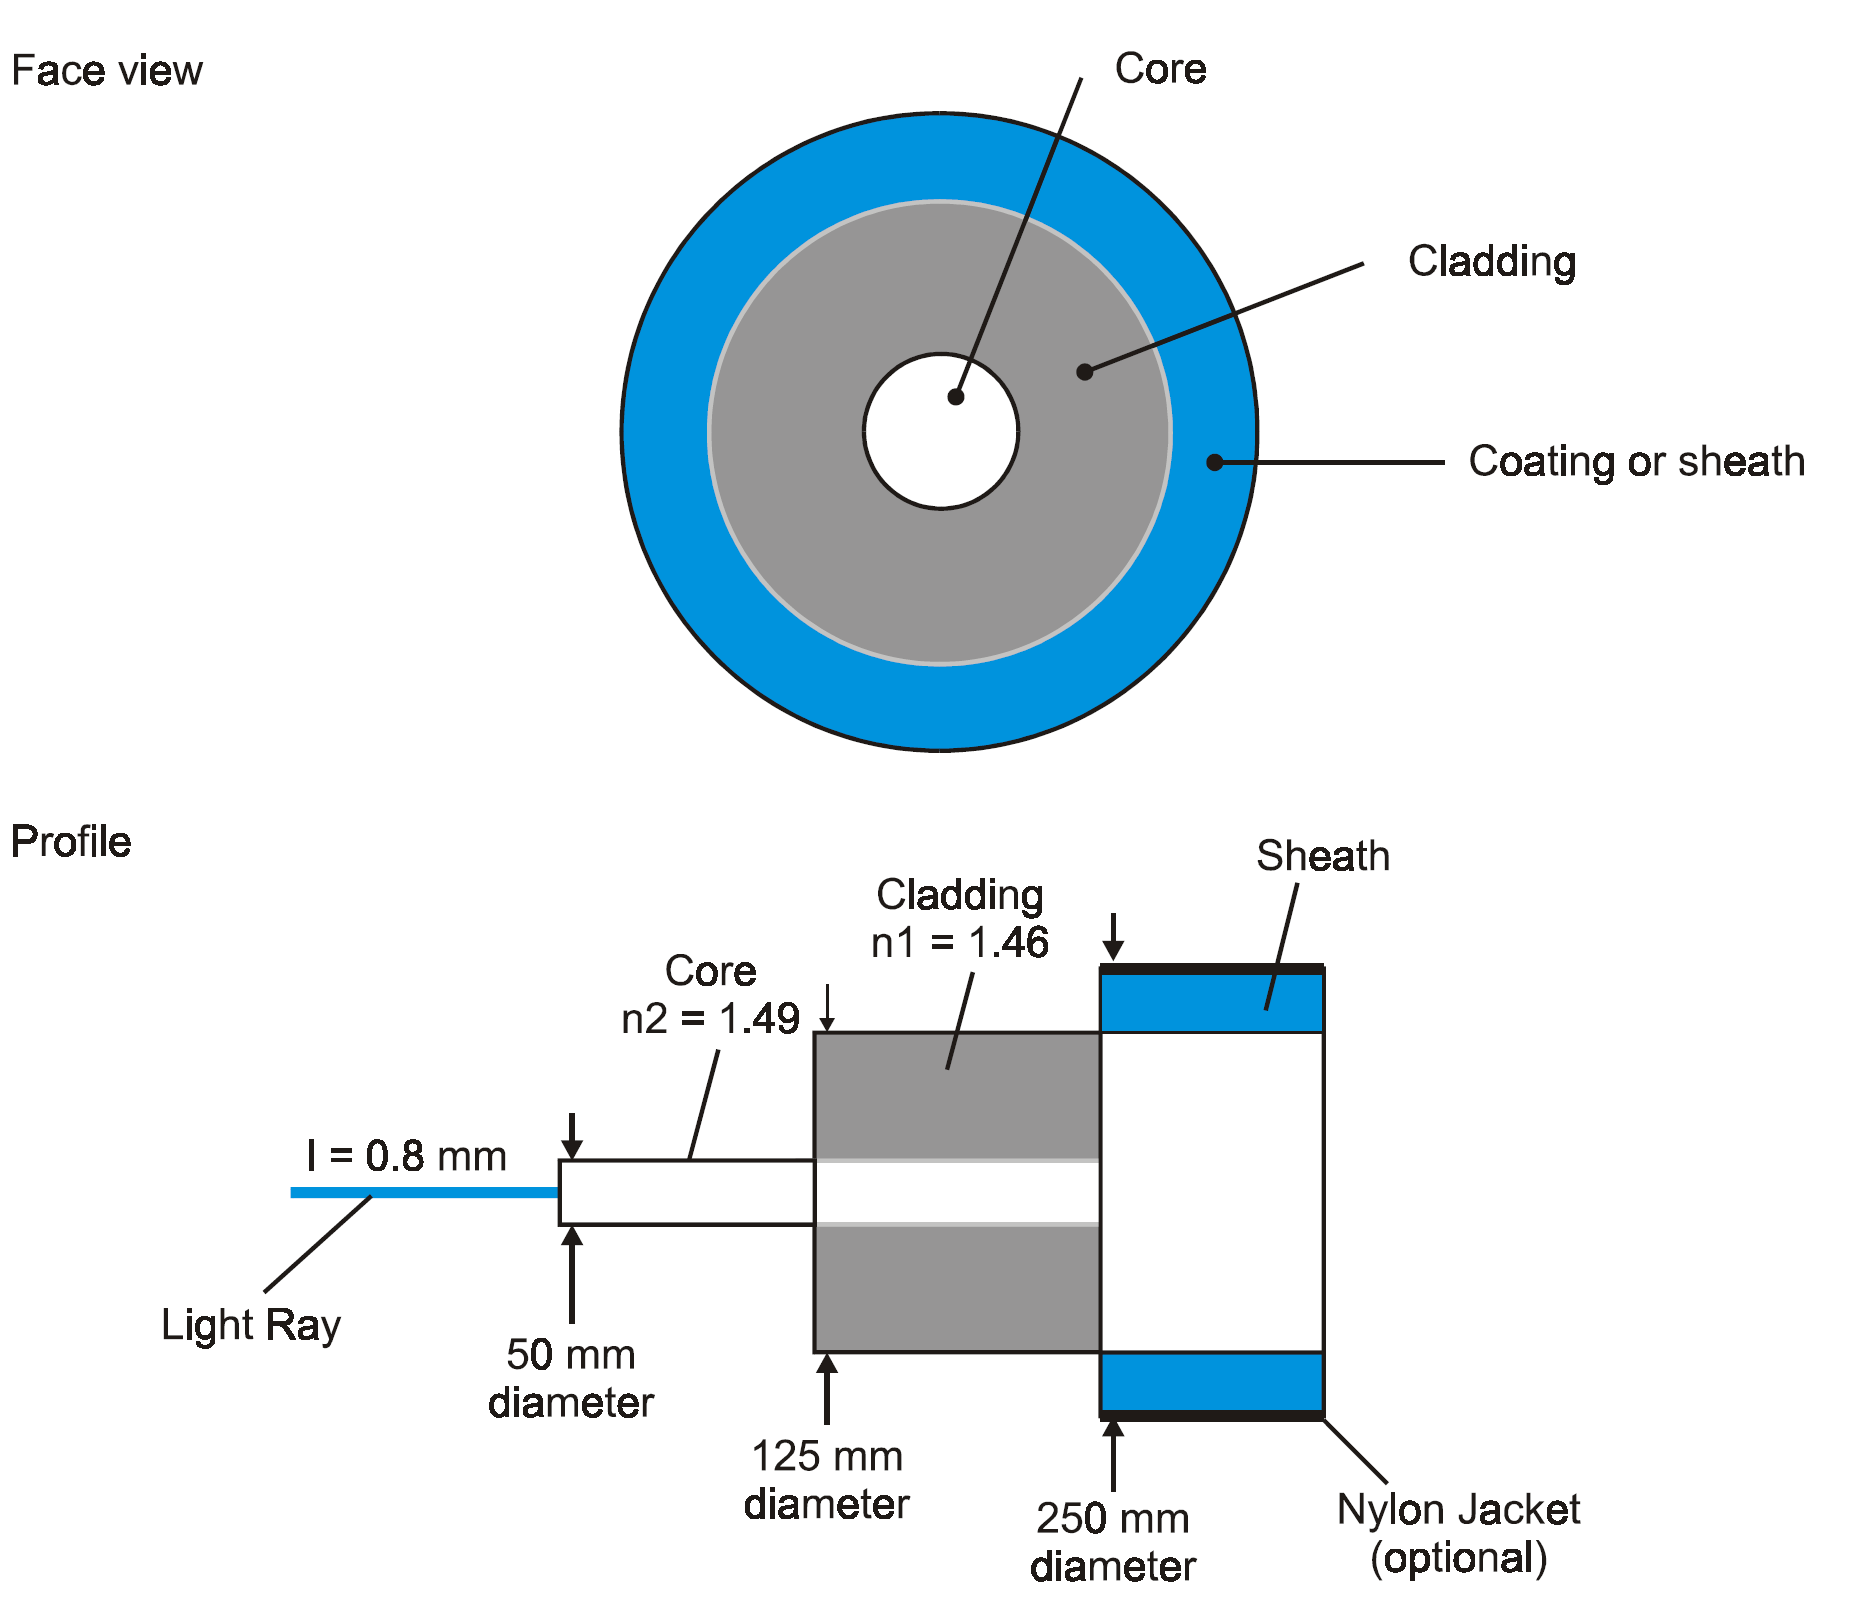
\includegraphics[width=\textwidth]{fig/fig35.png}	
%\end{figure}


\chapter{Projektbeskrivelse for Eksamensprojekt: IoT Smart House}
\section*{Formål}
Formålet med dette eksamensprojekt er at udvikle et IoT Smart House, hvor der redegøres for teknologikæden og anvendt IoT-teknologi. Projektet vil inkludere implementering og integration af forskellige sensorer og aktuatorer, kommunikationsprotokoller, datalagring, og et kontrolpanel ved hjælp af Node-RED. Projektet skal demonstreres i en 5-minutters videopræsentation, hvor løsningen beskrives og evalueres.

\section*{Projektindhold}

\subsection*{Teknologikæde}
Dette projekt vil udforske en komplet teknologikæde, der begynder med sensorer og aktuatorer forbundet til en ESP32-mikrocontroller. Data fra sensorerne vil blive behandlet og sendt videre ved hjælp af en eller flere kommunikationsprotokoller. Disse data vil blive lagret i en database, som f.eks. Firebase Realtime Database (RTDB), og præsenteret i et dashboard udviklet i Node-RED. Projektet vil også undersøge sikkerhedsaspekter af IoT-løsningen.

\subsection*{Anvendt IoT-teknologi}

\paragraph{Node-RED og Dashboard}
Node-RED vil blive brugt som et kontrolpanel til at overvåge og styre IoT-enhederne. Et brugervenligt dashboard vil blive udviklet for at visualisere data fra sensorer og give kontrol over aktuatorer.

\paragraph{Kommunikationsprotokoller}
To til tre kommunikationsprotokoller vil blive implementeret for at forbinde enhederne i Smart House. Eksempler kan være MQTT, HTTP, og Modbus, som vil blive anvendt til at overføre data mellem ESP32 og centrale systemer.

\paragraph{Data Lagring}
Data fra sensorerne vil blive sendt til en Firebase Realtime Database (RTDB), hvor de lagres for senere analyse og overvågning. Alternativt kan en anden database anvendes, afhængigt af projektets krav.

\subsection*{Prøveform og Præsentation}
Projektet vil blive præsenteret gennem en individuel videopræsentation, hvor de valgte teknologier og løsninger forklares og demonstreres. Videoen skal være ca. 5 minutter lang og skal tydeligt vise forståelsen af IoT-teknologi og dens anvendelse i et Smart House.

\subsection*{Opsummering}
Dette eksamensprojekt har til formål at udvikle og demonstrere en IoT-baseret Smart House-løsning, der integrerer flere teknologier, herunder Node-RED, kommunikationsprotokoller og datalagring. Projektet vil blive præsenteret i en videopræsentation, som viser de praktiske anvendelser af IoT i et moderne hjem.

\subsection*{Sensor \& aktuator}
IoT Smart House har et antal sensor og aktuatorer som er følgende:
\begin{itemize}
	\item DHT11 - Temperatur- og fugtighedssensor (tilsluttet IO17).
	\item PIR Motion Sensor - Bevægelsessensor (tilsluttet IO14).
	\item Gas Sensor - (tilsluttet IO23).
	\item Steam Sensor - (tilsluttet IO34).
	\item RFID Module - (tilsluttet via I2C).
	\item LED Module - Yellow LED (tilsluttet IO12).
	\item 6812RGB LED - RGB LED (tilsluttet IO26).
	\item Buzzer - (tilsluttet IO25).
	\item Servo Motor (Windows) - Styring af vinduer (tilsluttet IO5).
	\item Servo Motor (Doors) - Styring af døre (tilsluttet IO13).
	\item Left Button Module - Venstre knap (tilsluttet IO16).
	\item Right Button Module - Højre knap (tilsluttet IO27).
	\item Fan - (tilsluttet IO18 og IO19).
	\item LCD1602 Display - Tilsluttet via I2C.
\end{itemize}

\clearpage

\subsection*{Sensor \& aktuator kode}
\subsubsection*{DHT11 - Temperatur- og fugtighedssensor}
\begin{lstlisting}[language=C++]
	#include <DHT.h>
	
	// Define the DHTSensor class directly in the .ino file
	class DHTSensor {
		private:
		uint8_t pin;  // Pin number where the sensor is connected
		DHT dht;      // DHT object for handling the sensor
		
		public:
		// Constructor to initialize the DHTSensor with a pin and sensor type (DHT11/DHT22)
		DHTSensor(uint8_t p, uint8_t type) : pin(p), dht(p, type) {}
		
		// Method to initialize the sensor
		void begin() {
			dht.begin();
		}
		
		// Method to read temperature from the sensor
		float readTemperature() {
			float temp = dht.readTemperature();
			if (isnan(temp)) {
				Serial.println("Failed to read temperature!");
				return -1.0;
			}
			return temp;
		}
		
		// Method to read humidity from the sensor
		float readHumidity() {
			float humidity = dht.readHumidity();
			if (isnan(humidity)) {
				Serial.println("Failed to read humidity!");
				return -1.0;
			}
			return humidity;
		}
	};
	
	// Create an object of the DHTSensor class
	DHTSensor dhtSensor(17, DHT11);
	
	void setup() {
		Serial.begin(115200);   // Initialize serial communication at 115200 baud rate
		dhtSensor.begin();      // Initialize the DHT sensor
	}
	
	void loop() {
		// Read temperature and humidity from the sensor
		float temperature = dhtSensor.readTemperature();
		float humidity = dhtSensor.readHumidity();
		
		// Print temperature if it's valid
		if (temperature != -1.0) {
			Serial.print("Temperature: ");
			Serial.print(temperature);
			Serial.println(" C");
		}
		
		// Print humidity if it's valid
		if (humidity != -1.0) {
			Serial.print("Humidity: ");
			Serial.print(humidity);
			Serial.println(" %");
		}
		
		delay(2000);  // Wait 2 seconds between readings
	}
\end{lstlisting}
\clearpage
\subsubsection*{PIR Motion Sensor}
\begin{lstlisting}[language=C++]
	// Define the PIRSensor class directly in the .ino file
	class PIRSensor {
		private:
		uint8_t pin;  // Pin number where the PIR sensor is connected
		
		public:
		// Constructor to initialize the PIRSensor with a specific pin
		PIRSensor(uint8_t p) : pin(p) {
			pinMode(pin, INPUT);  // Set the PIR sensor pin as input
		}
		
		// Method to check if motion is detected by the PIR sensor
		bool isMotionDetected() {
			return digitalRead(pin) == HIGH;  // Return true if motion is detected
		}
	};
	
	// Create an object of the PIRSensor class
	PIRSensor pirSensor(14);
	
	void setup() {
		Serial.begin(115200);  // Initialize serial communication at 115200 baud rate
	}
	
	void loop() {
		// Check if motion is detected by the PIR sensor
		if (pirSensor.isMotionDetected()) {
			Serial.println("Motion detected!");  // Print a message if motion is detected
		} else {
			Serial.println("No motion.");  // Print a message if no motion is detected
		}
		
		delay(2000);  // Wait 2 seconds between checks
	}
\end{lstlisting}
\clearpage
\subsubsection*{Gas Sensor}
\begin{lstlisting}[language=C++]
	// Define the GasSensor class directly in the .ino file
	class GasSensor {
		private:
		uint8_t pin;  // Pin number where the Gas sensor is connected
		
		public:
		// Constructor to initialize the GasSensor with a specific pin
		GasSensor(uint8_t p) : pin(p) {
			pinMode(pin, INPUT);  // Set the Gas sensor pin as input
		}
		
		// Method to read the gas level from the sensor
		int readGasLevel() {
			return analogRead(pin);  // Return the analog value from the sensor
		}
	};
	
	// Create an object of the GasSensor class
	GasSensor gasSensor(23);
	
	void setup() {
		Serial.begin(115200);  // Initialize serial communication at 115200 baud rate
	}
	
	void loop() {
		// Read the gas level from the sensor
		int gasLevel = gasSensor.readGasLevel();
		Serial.print("Gas level: ");
		Serial.println(gasLevel);
		
		delay(2000);  // Wait 2 seconds between readings
	}
\end{lstlisting}
\clearpage	
\subsubsection*{Steam Sensor}
\begin{lstlisting}[language=C++]
	// Define the SteamSensor class directly in the .ino file
	class SteamSensor {
		private:
		uint8_t pin;  // Pin number where the Steam sensor is connected
		
		public:
		// Constructor to initialize the SteamSensor with a specific pin
		SteamSensor(uint8_t p) : pin(p) {
			pinMode(pin, INPUT);  // Set the Steam sensor pin as input
		}
		
		// Method to read the steam level from the sensor
		int readSteamLevel() {
			return analogRead(pin);  // Return the analog value from the sensor
		}
	};
	
	// Create an object of the SteamSensor class
	SteamSensor steamSensor(34);
	
	void setup() {
		Serial.begin(115200);  // Initialize serial communication at 115200 baud rate
	}
	
	void loop() {
		// Read the steam level from the sensor
		int steamLevel = steamSensor.readSteamLevel();
		Serial.print("Steam level: ");
		Serial.println(steamLevel);
		
		delay(2000);  // Wait 2 seconds between readings
	}
\end{lstlisting}
\clearpage
\subsubsection*{RFID Module}
\begin{lstlisting}[language=C++]
	#include <Wire.h>
	#include <MFRC522_I2C.h>
	
	// Define the RFIDModule class directly in the .ino file
	class RFIDModule {
		private:
		uint8_t address;  // I2C address for the RFID module
		MFRC522 mfrc522;
		
		public:
		// Constructor to initialize the RFIDModule with a specific I2C address
		RFIDModule(uint8_t addr) : address(addr), mfrc522(addr) {}
		
		// Method to initialize the RFID module
		void begin() {
			mfrc522.PCD_Init();
		}
		
		// Method to check if a new card is present and read its UID
		bool readCardUID() {
			if (!mfrc522.PICC_IsNewCardPresent() || ! mfrc522.PICC_ReadCardSerial()) {
				return false;
			}
			
			Serial.print("Card UID:");
			for (byte i = 0; i < mfrc522.uid.size; i++) {
				Serial.print(mfrc522.uid.uidByte[i] < 0x10 ? " 0" : " ");
				Serial.print(mfrc522.uid.uidByte[i], HEX);
			}
			Serial.println();
			return true;
		}
	};
	
	// Create an object of the RFIDModule class
	RFIDModule rfidModule(0x28);  // I2C address for the RFID module
	
	void setup() {
		Serial.begin(115200);  // Initialize serial communication at 115200 baud rate
		Wire.begin();          // Initialize I2C communication
		rfidModule.begin();    // Initialize RFID module
	}
	
	void loop() {
		// Check if a card is present and read its UID
		if (rfidModule.readCardUID()) {
			Serial.println("Card detected.");
		} else {
			Serial.println("No card detected.");
		}
		
		delay(1000);  // Wait 1 second between checks
	}
\end{lstlisting}
\clearpage
\subsubsection*{LED Module - Yellow LED}
\begin{lstlisting}[language=C++]
	// Define the LEDModule class directly in the .ino file
	class LEDModule {
		private:
		uint8_t pin;  // Pin number where the LED is connected
		
		public:
		// Constructor to initialize the LEDModule with a specific pin
		LEDModule(uint8_t p) : pin(p) {
			pinMode(pin, OUTPUT);  // Set the LED pin as output
		}
		
		// Method to turn on the LED
		void turnOn() {
			digitalWrite(pin, HIGH);  // Set the pin high to turn on the LED
		}
		
		// Method to turn off the LED
		void turnOff() {
			digitalWrite(pin, LOW);  // Set the pin low to turn off the LED
		}
	};
	
	// Create an object of the LEDModule class
	LEDModule yellowLED(12);
	
	void setup() {
		Serial.begin(115200);  // Initialize serial communication at 115200 baud rate
	}
	
	void loop() {
		// Turn the LED on and off with a 1-second delay
		yellowLED.turnOn();
		Serial.println("Yellow LED is ON");
		delay(1000);
		
		yellowLED.turnOff();
		Serial.println("Yellow LED is OFF");
		delay(1000);
	}
\end{lstlisting}
\clearpage
\subsubsection*{Buzzer}
\begin{lstlisting}[language=C++]
	// Define the Buzzer class directly in the .ino file
	class Buzzer {
		private:
		uint8_t pin;  // Pin number where the Buzzer is connected
		
		public:
		// Constructor to initialize the Buzzer with a specific pin
		Buzzer(uint8_t p) : pin(p) {
			pinMode(pin, OUTPUT);  // Set the Buzzer pin as output
		}
		
		// Method to turn on the Buzzer
		void turnOn() {
			digitalWrite(pin, HIGH);  // Set the pin high to turn on the Buzzer
		}
		
		// Method to turn off the Buzzer
		void turnOff() {
			digitalWrite(pin, LOW);  // Set the pin low to turn off the Buzzer
		}
		
		// Method to make the Buzzer beep for a specified duration
		void beep(unsigned int duration) {
			turnOn();
			delay(duration);
			turnOff();
		}
	};
	
	// Create an object of the Buzzer class
	Buzzer buzzer(25);
	
	void setup() {
		Serial.begin(115200);  // Initialize serial communication at 115200 baud rate
	}
	
	void loop() {
		// Make the Buzzer beep with a 500ms duration
		buzzer.beep(500);
		Serial.println("Buzzer beeped");
		delay(2000);  // Wait 2 seconds between beeps
	}
\end{lstlisting}
\clearpage
\subsubsection*{Servo Motor}
Efersom servo motor er den samme kode for både dør og vindue så laves kun en klasse, men fordi det er en klasse så kan koden genbruges.
\begin{lstlisting}[language=C++]
	#include <ESP32Servo.h>
	
	// Define the ServoMotor class directly in the .ino file
	class ServoMotor {
		private:
		Servo servo;       // Servo object
		uint8_t pin;       // Pin number where the servo is connected
		int position;      // Current position of the servo
		
		public:
		// Constructor to initialize the ServoMotor with a specific pin
		ServoMotor(uint8_t p) : pin(p), position(0) {}
		
		// Method to attach the servo to the specified pin
		void begin() {
			servo.attach(pin);
		}
		
		// Method to set the position of the servo within the range 0-180 degrees
		void setPosition(int pos) {
			if (pos >= 0 && pos <= 180) {
				position = pos;
				servo.write(position);  // Move servo to the specified position
				Serial.print("Servo moved to: ");
				Serial.print(position);
				Serial.println(" degrees");
			} else {
				Serial.println("Error: Position out of range (0-180)");
			}
		}
		
		// Method to get the current position of the servo
		int getPosition() {
			return position;
		}
	};
	
	// Create an object of the ServoMotor class
	ServoMotor myServo(5);
	
	void setup() {
		Serial.begin(115200);  // Initialize serial communication at 115200 baud rate
		myServo.begin();       // Attach the servo motor
		myServo.setPosition(90);  // Start with the servo at 90 degrees
	}
	
	void loop() {
		// Example of setting the servo to different angles
		delay(2000);
		myServo.setPosition(45);  // Move the servo to 45 degrees
		delay(2000);
		myServo.setPosition(135); // Move 
	\end{lstlisting}
	\clearpage
	\subsubsection*{Button Module}
	Efersom servo motor er den samme kode for både dør og vindue så laves kun en klasse, men fordi det er en klasse så kan koden genbruges.
	\begin{lstlisting}[language=C++]
		#include <Arduino.h>
		
		volatile bool buttonStateChanged = false;  // Flag to indicate button state change
		
		class ButtonModule {
			private:
			uint8_t pin;  // Pin number where the button is connected
			int buttonState;  // Variable to store the current state of the button
			
			public:
			// Constructor to initialize the ButtonModule with a specific pin
			ButtonModule(uint8_t p) : pin(p), buttonState(HIGH) {
				pinMode(pin, INPUT_PULLUP);  // Set the button pin as input with internal pull-up
				attachInterrupt(digitalPinToInterrupt(pin), handleInterrupt, CHANGE);  // Attach interrupt to handle button state change
			}
			
			// Method to check if the button state changed
			int getState() {
				if (buttonStateChanged) {
					buttonStateChanged = false;  // Reset the flag after reading
					buttonState = digitalRead(pin);  // Read and return the current state of the button
				}
				return buttonState;  // Return the last known state if no change
			}
			
			// Interrupt Service Routine to handle the button state change
			static void handleInterrupt() {
				buttonStateChanged = true;  // Set the flag to indicate button state change
			}
		};
		
		// Create an object of the ButtonModule class
		ButtonModule button(16);  // Replace 16 with the actual pin number if necessary
		
		void setup() {
			Serial.begin(115200);  // Initialize serial communication at 115200 baud rate
		}
		
		void loop() {
			// Check if the button state changed and print the result
			int buttonState = button.getState();
			Serial.print("Button state: ");
			Serial.println(buttonState == LOW ? "Pressed" : "Released");
			
			delay(100);  // Small delay for debounce
		}
	\end{lstlisting}
	\clearpage
	\subsubsection*{Fan}
	\begin{lstlisting}[language=C++]
		#include <Arduino.h>
		
		class Fan {
			private:
			uint8_t pinIn1;  // Pin number for IN1 on the fan driver
			uint8_t pinIn2;  // Pin number for IN2 on the fan driver
			
			public:
			// Constructor to initialize the Fan with specific pins
			Fan(uint8_t in1, uint8_t in2) : pinIn1(in1), pinIn2(in2) {
				pinMode(pinIn1, OUTPUT);  // Set pinIn1 as output
				pinMode(pinIn2, OUTPUT);  // Set pinIn2 as output
				control(LOW);             // Ensure the fan is off at the start
			}
			
			// Method to control the fan with HIGH or LOW
			void control(int state) {
				if (state == HIGH) {
					digitalWrite(pinIn1, HIGH);  // Set IN1 high
					digitalWrite(pinIn2, LOW);   // Set IN2 low
					Serial.println("Fan is ON");
				} else {
					digitalWrite(pinIn1, LOW);   // Set IN1 low
					digitalWrite(pinIn2, LOW);   // Set IN2 low
					Serial.println("Fan is OFF");
				}
			}
		};
		
		// Create an object of the Fan class
		Fan fan(18, 19);  // Replace 18 and 19 with the actual pin numbers if necessary
		
		void setup() {
			Serial.begin(115200);  // Initialize serial communication at 115200 baud rate
			fan.control(LOW);      // Start with the fan off
		}
		
		void loop() {
			delay(2000);
			fan.control(HIGH);  // Turn the fan on
			delay(2000);
			fan.control(LOW);   // Turn the fan off
		}
	\end{lstlisting}
	
	\subsubsection*{LCD1602 Display}
	\begin{lstlisting}[language=C++]
		#include <Wire.h>
		#include <LiquidCrystal_I2C.h>
		
		class LCD1602Display {
			private:
			LiquidCrystal_I2C lcd;  // LCD object
			
			public:
			// Constructor to initialize the LCD with the I2C address
			LCD1602Display(uint8_t lcdAddr) : lcd(lcdAddr, 16, 2) {
				lcd.init();  // Initialize the LCD
				lcd.backlight();  // Turn on the backlight
			}
			
			// Method to print text on the first row
			void printLine1(const char* row1) {
				lcd.setCursor(0, 0);  // Set cursor to the first row, first column
				lcd.print("                "); // Clear the line
				lcd.setCursor(0, 0);  // Set cursor back to the first row
				lcd.print(row1);  // Print text on the first row
			}
			
			// Method to print text on the second row
			void printLine2(const char* row2) {
				lcd.setCursor(0, 1);  // Set cursor to the second row, first column
				lcd.print("                "); // Clear the line
				lcd.setCursor(0, 1);  // Set cursor back to the second row
				lcd.print(row2);  // Print text on the second row
			}
		};
		
		// Create an object of the LCD1602Display class with I2C address 0x27
		LCD1602Display lcdDisplay(0x27);
		
		void setup() {
			// Initial text on the LCD
			lcdDisplay.printLine1("Hello, World!");
			lcdDisplay.printLine2("Welcome!");
		}
		
		void loop() {
			// Example: Change text on the LCD every 5 seconds
			delay(5000);
			lcdDisplay.printLine1("Line 1 Updated");
			lcdDisplay.printLine2("Line 2 Updated");
			
			delay(5000);
			lcdDisplay.printLine1("Another Line 1");
			lcdDisplay.printLine2("Another Line 2");
		}
	\end{lstlisting}
	
	\subsection*{Alt kode}
	\begin{lstlisting}
		
	\end{lstlisting}
	
	\part{Opgaver}
\chapter{C++ Basic}
\section{\texttt{Delay()} i Arduino}

\subsection*{Formål}
Formålet med dette afsnit er at introducere og forklare, hvordan \texttt{delay()}-funktionen fungerer i Arduino-programmering, herunder dens fordele og ulemper, samt hvordan man kan anvende funktionen effektivt i projekter.

\subsection*{Introduktion}
\texttt{delay()} er en indbygget funktion i Arduino-programmeringssproget, der bruges til at skabe en pause i kodeudførelsen i en bestemt periode. Funktionen tager en enkelt parameter: den tid, programmet skal vente, angivet i millisekunder.

\subsection*{Hvad er \texttt{delay()}?}
\texttt{delay()}-funktionen bruges til at stoppe programudførelsen for en angivet tid, hvilket kan være nyttigt i mange situationer, såsom at blinke en LED eller skabe tidsbaserede sekvenser. Her er et eksempel på, hvordan \texttt{delay()} kan bruges til at tænde og slukke den indbyggede LED på et Arduino-board:

\begin{lstlisting}[language=C++, caption={Using the \texttt{delay()} function with the built-in LED.}]
	void setup() {
		pinMode(LED_BUILTIN, OUTPUT); 
		// Set the built-in LED as OUTPUT
	}
	
	void loop() {
		digitalWrite(LED_BUILTIN, HIGH); 
		// Turn on the built-in LED
		delay(1000);                     
		// Wait for 1000 milliseconds (1 second)
		digitalWrite(LED_BUILTIN, LOW);  
		// Turn off the built-in LED
		delay(1000);                     
		// Wait for 1000 milliseconds (1 second)
	}
\end{lstlisting}

\subsection*{Opgaver med \texttt{delay()}}

\subsubsection*{Opgave 1: Blinkende LED}
\textbf{Formål:}\\
Lær at styre den indbyggede LED på en ESP32 eller Arduino-board ved hjælp af \texttt{delay()}-funktionen.

\textbf{Opgave:}
\begin{enumerate}
	\item Tænd den indbyggede LED i 2 sekunder.
	\item Sluk den indbyggede LED i 3 sekunder.
	\item Gentag trin 1 og 2 kontinuerligt.
\end{enumerate}

\subsubsection*{Opgave 2: Sekvens af LED'er}
\textbf{Formål:}\\
Lær at styre flere LED'er sekventielt ved hjælp af \texttt{delay()}-funktionen.

\textbf{Materialer:}
\begin{itemize}
	\item 3 LED'er
	\item 3 220-ohm modstande
	\item Breadboard og jumperkabler
\end{itemize}

\textbf{Opgave:}
\begin{enumerate}
	\item Tilslut de tre LED'er til henholdsvis pin 2, 3 og 4 på dit board.
	\item Tænd LED 1 (pin 2) i 1 sekund, og sluk den derefter.
	\item Umiddelbart efter LED 1 slukker, tænd LED 2 (pin 3) i 1 sekund, og sluk den derefter.
	\item Umiddelbart efter LED 2 slukker, tænd LED 3 (pin 4) i 1 sekund, og sluk den derefter.
	\item Gentag trin 2-4 kontinuerligt.
\end{enumerate}

\subsubsection*{Opgave 3: Trafiklys-simulator}
\textbf{Formål:}\\
Simulere et trafiklys ved hjælp af \texttt{delay()}-funktionen.

\textbf{Materialer:}
\begin{itemize}
	\item Rød, gul og grøn LED
	\item 3 220-ohm modstande
	\item Breadboard og jumperkabler
\end{itemize}

\textbf{Opgave:}
\begin{enumerate}
	\item Tilslut de tre LED'er til henholdsvis pin 2 (rød), 3 (gul) og 4 (grøn) på dit board.
	\item Tænd den røde LED i 5 sekunder, og sluk den derefter.
	\item Tænd den gule LED i 1,5 sekund, og sluk den derefter.
	\item Tænd den grønne LED i 4 sekunder, og sluk den derefter.
	\item Gentag trin 2-4 kontinuerligt.
\end{enumerate}

\subsection*{Konklusion}
\texttt{delay()}-funktionen er en simpel, men kraftfuld måde at introducere tidsbaserede handlinger i dine Arduino-projekter. Selvom det er en nem måde at implementere pauser i kodeudførelsen, kan det også føre til udfordringer, såsom at blokere andre processer. I de kommende kapitler vil vi udforske alternative metoder til tidsstyring, som giver mere fleksibilitet og effektivitet.

\subsection*{Løsningsforslag}

\subsubsection*{Løsningsforslag for Opgave 1}
\begin{lstlisting}[language=C++]
	void setup() {
		pinMode(LED_BUILTIN, OUTPUT);
	}
	
	void loop() {
		digitalWrite(LED_BUILTIN, HIGH);  // Turn on the built-in LED
		delay(2000);                      // Wait for 2000 ms or 2 seconds
		digitalWrite(LED_BUILTIN, LOW);   // Turn off the built-in LED
		delay(3000);                      // Wait for 3000 ms or 3 seconds
	}
\end{lstlisting}

\subsubsection*{Løsningsforslag for Opgave 2}
\begin{lstlisting}[language=C++]
	void setup() {
		pinMode(2, OUTPUT);
		pinMode(3, OUTPUT);
		pinMode(4, OUTPUT);
	}
	
	void loop() {
		digitalWrite(2, HIGH);  
		delay(1000);                      
		digitalWrite(2, LOW);   
		
		digitalWrite(3, HIGH);  
		delay(1000);                      
		digitalWrite(3, LOW);   
		
		digitalWrite(4, HIGH);  
		delay(1000);                      
		digitalWrite(4, LOW);   
	}
\end{lstlisting}

\subsubsection*{Løsningsforslag for Opgave 3}
\begin{lstlisting}[language=C++]
	void setup() {
		pinMode(2, OUTPUT);  // Red LED
		pinMode(3, OUTPUT);  // Yellow LED
		pinMode(4, OUTPUT);  // Green LED
	}
	
	void loop() {
		digitalWrite(2, HIGH);  // Turn on red LED
		delay(5000);            // Wait for 5000 ms or 5 seconds
		digitalWrite(2, LOW);   // Turn off red LED
		
		digitalWrite(3, HIGH);  // Turn on yellow LED
		delay(1500);            // Wait for 1500 ms or 1.5 seconds
		digitalWrite(3, LOW);   // Turn off yellow LED
		
		digitalWrite(4, HIGH);  // Turn on green LED
		delay(4000);            // Wait for 4000 ms or 4 seconds
		digitalWrite(4, LOW);   // Turn off green LED
	}
\end{lstlisting}

\section{Trykknapper}
\subsubsection*{Introduktion}
Pull-up og pull-down modstande er essentielle for at sikre, at en digital indgang får en klart defineret værdi, uanset om den er åben eller kortsluttet. Dette er særligt vigtigt for at undgå tilfældige omskiftninger på grund af støj.

\subsubsection*{Pull-Up Modstand}
En pull-up modstand er forbundet til en digital indgang og Vcc. Når trykknappen ikke er aktiveret (ingen forbindelse), vil digital indgang læse "HIGH" på grund af pull-up modstanden. Når trykknappen er trykket, vil den digitale indgang læse "LOW", fordi knappen nu er kortsluttet til jorden.

\subsubsection*{Pull-Down Modstand}
Tilsvarende er en pull-down modstand forbundet til en digital indgang og jord. Når trykknappen ikke er aktiveret, vil den digitale indgang læse "LOW" på grund af pull-down modstanden. Når trykknappen er trykket, vil den digitale indgang læse "HIGH", da knappen nu er kortsluttet til Vcc.

\subsubsection*{Opgaver}
\begin{itemize}
	\item \textbf{Blinkende LED ved Tryk:} Skriv et program, hvor den indbyggede LED blinker, når trykknappen er trykket, og er slukket, når knappen ikke er trykket.
	\item \textbf{Veksling ved Tryk:} Skriv et program, hvor den indbyggede LED skifter mellem tændt og slukket hver gang trykknappen trykkes og frigives.
	\item \textbf{Tryk Tæller:} Skriv et program, der tæller antallet af gange, trykknappen er blevet trykket. Hver gang knappen trykkes, skal den indbyggede LED blinke svarende til det aktuelle antal tryk.
\end{itemize}

\subsubsection*{Konklusion}
For at sikre stabil aflæsning af trykknapper i digitale kredsløb er det vigtigt at anvende enten pull-up eller pull-down modstande. Dette eliminerer usikkerhed og sikrer, at mikrocontrolleren korrekt kan aflæse, om en knap er blevet trykket eller ej.

\clearpage

\subsection*{Løsningsforslag}

\subsubsection*{Blinkende LED ved Tryk}
Når trykknappen er trykket, skal den indbyggede LED tænde, og når den ikke er trykket, skal LED'en være slukket.
\begin{lstlisting}[language=C++]
	int buttonPin = 2;  // assume the button is connected to pin 2
	int ledPin = LED_BUILTIN;  // built-in LED
	
	void setup() {
		pinMode(buttonPin, INPUT_PULLUP);
		pinMode(ledPin, OUTPUT);
	}
	
	void loop() {
		int buttonState = digitalRead(buttonPin);
		if (buttonState == LOW) {   // If the button is pressed (due to INPUT_PULLUP)
			digitalWrite(ledPin, HIGH);
		} else {
			digitalWrite(ledPin, LOW); // If the button is not pressed
		}
	}
\end{lstlisting}

\subsubsection*{Veksling ved Tryk}
LED'en skifter mellem tændt og slukket hver gang trykknappen trykkes og frigives.
\begin{lstlisting}[language=C++]
	int buttonPin = 2;
	int ledPin = LED_BUILTIN;
	bool lastButtonState = HIGH;
	bool ledState = LOW;
	
	void setup() {
		pinMode(buttonPin, INPUT_PULLUP);
		pinMode(ledPin, OUTPUT);
	}
	
	void loop() {
		bool currentButtonState = digitalRead(buttonPin);
		
		if (currentButtonState == LOW && lastButtonState == HIGH) {
			ledState = !ledState;
			digitalWrite(ledPin, ledState);
			delay(50); // debounce
		}
		lastButtonState = currentButtonState;
	}
\end{lstlisting}

\subsubsection*{Tryk Tæller}
Hver gang knappen trykkes, blinker LED'en svarende til det aktuelle antal tryk.
\begin{lstlisting}[language=C++]
	int buttonPin = 2;
	int ledPin = LED_BUILTIN;
	bool lastButtonState = HIGH;
	int pressCount = 0;
	
	void setup() {
		pinMode(buttonPin, INPUT_PULLUP);
		pinMode(ledPin, OUTPUT);
	}
	
	void loop() {
		bool currentButtonState = digitalRead(buttonPin);
		
		if (currentButtonState == LOW && lastButtonState == HIGH) {
			pressCount++;
			for(int i = 0; i < pressCount; i++) {
				digitalWrite(ledPin, HIGH);
				delay(250);
				digitalWrite(ledPin, LOW);
				delay(250);
			}
			delay(50); // debounce
		}
		lastButtonState = currentButtonState;
	}
\end{lstlisting}
Med disse løsningsforslag vil din Arduino reagere forskelligt på trykknappens tilstand afhængigt af det specifikke program, du har valgt.

\section{DHT11 Sensor}
\subsection*{Formål}
Formålet med dette afsnit er at introducere læseren til DHT11-føleren, en prisvenlig og effektiv enhed til måling af temperatur og luftfugtighed. Ved at kombinere teoretisk viden med praktisk anvendelse vil læseren få hands-on erfaring med at opsætte, programmere og aflæse data fra DHT11 ved hjælp af ESP32 mikrocontrolleren. De medfølgende opgaver er designet til at styrke forståelsen af, hvordan DHT11-føleren fungerer, samt hvordan data kan bearbejdes og anvendes i forskellige scenarier. Derudover inkorporeres matematiske koncepter for at styrke integrationen af programmering og matematik i realverdenen. Gennem dette afsnit vil læseren opnå en solid forståelse for både hardware- og softwareaspekterne ved at arbejde med temperatur- og fugtighedsfølere i indlejrede systemer.

\subsection*{Introduktion til DHT11-føleren}
DHT11 er en populær temperatur- og luftfugtighedsføler, som er både omkostningseffektiv og nem at bruge. Den fungerer ved at måle omgivende luft og give digitale signaler, der kan læses fra et mikrocontroller board som ESP32.

\subsection*{Opsætning af DHT11 med ESP32}
\begin{enumerate}
	\item Tilslut DHT11-følerens VCC og GND til ESP32's 3,3V og GND henholdsvis.
	\item Tilslut data-pinden fra DHT11-føleren til en valgfri GPIO-pin på ESP32.
	\item Installér det nødvendige bibliotek til DHT11 ved at benytte PlatformIO's bibliotekshåndtering eller Arduino IDE's bibliotekshåndtering.
\end{enumerate}

\subsection*{Opgaver}
\begin{itemize}
	\item \textbf{Temperature Alarm:} Write a program that turns on the built-in LED if the temperature exceeds 25 degrees Celsius.
	\item \textbf{Humidity Difference Calculator:} Given that the maximum comfortable humidity level for a person is \(X\%\), write a program that calculates the difference between the current humidity and \(X\%\) and prints this value.
	\item \textbf{Temperature Converter:} Write a program that converts the measured temperature from Celsius to Fahrenheit and prints both values.
\end{itemize}

\subsection*{Konklusion}
Gennem denne vejledning har vi dykket ned i, hvordan DHT11-føleren fungerer og kan integreres med ESP32 for at aflæse omgivelsens temperatur og fugtighed. Denne viden er afgørende for mange IoT-applikationer, især dem, der fokuserer på klimakontrol, landbrug eller generel miljøovervågning.
\newline\newline\noindent
Med korrekt integration og programmering er DHT11 en pålidelig kilde til miljødata. Kombineret med matematisk analyse har vi også set, hvordan man kan manipulere og bruge disse data til at drage konklusioner eller lave forudsigelser.
\newline\newline\noindent
For dem, der ønsker at gå videre, kan yderligere eksperimenter og udviklingsprojekter med DHT11 og andre sensorer udforske, hvordan disse teknologier kan integreres i større systemer eller anvendes til at løse specifikke tekniske udfordringer.
\subsection*{Løsningsforslag}
\begin{itemize}
	\item \textbf{Temperature Alarm:} 
	\begin{lstlisting}[language=C++]
		#include <DHT.h>
		#define DHTPIN <Your GPIO pin>
		#define DHTTYPE DHT11
		DHT dht(DHTPIN, DHTTYPE);
		
		void setup() {
			dht.begin();
			pinMode(LED_BUILTIN, OUTPUT);
		}
		
		void loop() {
			float temp = dht.readTemperature();
			if (temp > 25) {
				digitalWrite(LED_BUILTIN, HIGH);
			} else {
				digitalWrite(LED_BUILTIN, LOW);
			}
		}
	\end{lstlisting}
	
	\item \textbf{Humidity Difference Calculator:}
	\begin{lstlisting}[language=C++]
		#include <DHT.h>
		#define DHTPIN <Your GPIO pin>
		#define DHTTYPE DHT11
		#define MAX_HUMIDITY X
		DHT dht(DHTPIN, DHTTYPE);
		
		void setup() {
			dht.begin();
			Serial.begin(9600);
		}
		
		void loop() {
			float humidity = dht.readHumidity();
			float diff = humidity - MAX_HUMIDITY;
			Serial.println(diff);
			delay(2000);
		}
	\end{lstlisting}
	
	\item \textbf{Temperature Converter:} 
	\begin{lstlisting}[language=C++]
		#include <DHT.h>
		#define DHTPIN <Your GPIO pin>
		#define DHTTYPE DHT11
		DHT dht(DHTPIN, DHTTYPE);
		
		void setup() {
			dht.begin();
			Serial.begin(9600);
		}
		
		void loop() {
			float tempC = dht.readTemperature();
			float tempF = tempC * 1.8 + 32;
			Serial.print("Temperature in C: "); Serial.println(tempC);
			Serial.print("Temperature in F: "); Serial.println(tempF);
			delay(2000);
		}
	\end{lstlisting}
\end{itemize}

\section{PIR Sensors}

\subsection*{Formål}
Formålet med dette afsnit er at introducere læseren til PIR-sensorer, en pålidelig teknologi til detektion af bevægelse baseret på infrarød stråling. Vi vil undersøge, hvordan PIR-sensorer arbejder, hvordan de kan integreres med ESP32 mikrocontrolleren, og hvordan de anvendes i praksis for at skabe bevægelsesaktiverede systemer. Dette vil suppleres med en række opgaver, der kombinerer tekniske og matematiske koncepter for at forstærke forståelsen af dette område.

\subsection*{Introduktion til PIR-sensorer}
En PIR-sensor (Passive Infrared-sensor) er en elektronisk sensor, der måler infrarødt (IR) lys, som udsendes fra genstande i dens synsfelt. De mest almindeligt anvendte typer af PIR-sensorer bruges i bevægelsesdetekteringssystemer som alarmer og belysning.

\subsection*{Opsætning af PIR-sensor med ESP32}
\begin{enumerate}
	\item Tilslut PIR-sensorens VCC og GND til ESP32's 3,3V og GND henholdsvis.
	\item Tilslut data-pinden fra PIR-sensoren til en valgfri GPIO-pin på ESP32.
	\item Initialiser GPIO-pinden i INPUT-tilstand i din kode.
\end{enumerate}

\subsection*{Opgaver}
\begin{itemize}
	\item \textbf{Motion Alarm:} Write a program that turns on the built-in LED if motion is detected by the PIR sensor.
	\item \textbf{Motion Time Calculator:} Record the time of the last five detected motions. Calculate the time intervals between them and print the average.
	\item \textbf{Alarm Counter:} Write a program that counts the number of times motion is detected within a given time period, such as 10 minutes.
\end{itemize}

\subsection*{Konklusion}
PIR-sensorer er essentielle i mange IoT- og automatiseringsprojekter, hvor bevægelsesdetektering er nødvendig. Ved korrekt integration med ESP32 kan man skabe intelligente systemer, der reagerer på menneskelig eller dyrisk bevægelse. Gennem denne vejledning og de tilhørende opgaver skulle læseren gerne have opnået en solid forståelse for, hvordan man opsætter, programmerer og drager nytte af PIR-sensorer.

\clearpage

\subsection*{Løsningsforslag}

\subsubsection*{Motion Alarm}
The built-in LED should turn on when motion is detected and turn off when no motion is detected.
\begin{lstlisting}[language=C++]
	#define PIRPIN <Your GPIO pin>
	void setup() {
		pinMode(PIRPIN, INPUT);
		pinMode(LED_BUILTIN, OUTPUT);
	}
	void loop() {
		int pirState = digitalRead(PIRPIN);
		if (pirState == HIGH) {
			digitalWrite(LED_BUILTIN, HIGH);
		} else {
			digitalWrite(LED_BUILTIN, LOW);
		}
	}
\end{lstlisting}

\subsubsection*{Motion Time Calculator}
This program records the time of the last five detected motions and calculates the average time interval between them.
\begin{lstlisting}[language=C++]
	#define PIRPIN <Your GPIO pin>
	unsigned long lastDetectedTimes[5] = {0, 0, 0, 0, 0};
	int currentIndex = 0;
	
	void setup() {
		pinMode(PIRPIN, INPUT);
		Serial.begin(9600);
	}
	
	void loop() {
		int pirState = digitalRead(PIRPIN);
		if (pirState == HIGH) {
			unsigned long currentTime = millis();
			lastDetectedTimes[currentIndex] = currentTime;
			currentIndex = (currentIndex + 1) % 5;
			
			unsigned long intervalSum = 0;
			for (int i = 1; i < 5; i++) {
				intervalSum += (lastDetectedTimes[i] - lastDetectedTimes[i - 1]);
			}
			float averageInterval = intervalSum / 4.0;
			Serial.println("Average interval: " + String(averageInterval) + " ms");
			delay(1000);  // Wait to avoid multiple detections
		}
	}
\end{lstlisting}

\subsubsection*{Alarm Counter}
This program counts the number of times motion is detected within a given time period, such as 10 minutes.
\begin{lstlisting}[language=C++]
	#define PIRPIN <Your GPIO pin>
	unsigned long startTime;
	int movementCount = 0;
	const unsigned long TEN_MINUTES = 10 * 60 * 1000;
	
	void setup() {
		pinMode(PIRPIN, INPUT);
		Serial.begin(9600);
		startTime = millis();
	}
	
	void loop() {
		if (millis() - startTime >= TEN_MINUTES) {
			Serial.println("Number of motions in the last 10 minutes: " + String(movementCount));
			movementCount = 0;
			startTime = millis();
		}
		
		int pirState = digitalRead(PIRPIN);
		if (pirState == HIGH) {
			movementCount++;
			delay(1000);  // Wait to avoid multiple detections
		}
	}
\end{lstlisting}

\section{RFID Teknologi}

\subsection*{Formål}
Formålet med dette afsnit er at introducere læseren for RFID-teknologi og den typiske anvendelse af en RFID-kortlæser, som MFRC522, sammen med en ESP32-mikrocontroller. Afsnittet giver en dybdegående forståelse af, hvordan man kan programmere og interagere med RFID-tags ved hjælp af ESP32, og hvordan disse tags kan bruges i daglige applikationer som adgangskontrol, identifikation og sporing.

\subsection*{Introduktion til RFID Kortlæseren}
RFID står for Radio Frequency Identification. Med RFID kan man trådløst identificere og spore tags, der er fastgjort til objekter. Kortlæseren, som MFRC522, bruger elektromagnetiske felter til automatisk at identificere og spore tags, som indeholder lagret information.

\subsection*{Opsætning af MFRC522 med ESP32}
\begin{enumerate}
	\item Tilslut MFRC522's VCC, RST, GND til ESP32's 3,3V, valgfri RESET pin og GND henholdsvis.
	\item Tilslut MISO, MOSI, SCK og SDA (SS) til ESP32's relevante SPI-pins.
	\item Installér det nødvendige bibliotek (f.eks., MFRC522 library) via PlatformIO eller Arduino IDE.
\end{enumerate}

\subsection*{Opgaver}
\begin{itemize}
	\item \textbf{Basic Card Reading:} Write a program that reads an RFID tag and prints its unique ID (UID) to the serial monitor.
	\item \textbf{Access Control:} Design a system where only specific RFID tags can turn on an LED. All other tags should turn off the LED.
	\item \textbf{Card Reading with Time:} Write a program that prints the exact time an RFID tag was scanned.
\end{itemize}

\subsection*{Konklusion}
Med denne vejledning har vi opnået grundlæggende viden om RFID-teknologi og dens mange applikationer, specifikt ved at integrere MFRC522-kortlæseren med ESP32-mikrocontrolleren. Teknologien bag RFID kan drastisk forbedre automatiserings- og identifikationsprocesserne i mange industrier, og forståelsen af dens grundlæggende funktionsmåde er essentiel for moderne elektronikentusiaster og ingeniører.

\clearpage

\subsection*{Løsningsforslag}
Her er løsningsforslagene til de stillede opgaver:

\subsubsection*{Basic Card Reading}

\begin{lstlisting}[language=C++, caption=Basic Card Reading Solution]
	#include <MFRC522.h>
	
	MFRC522 mfrc522(SS_PIN, RST_PIN);  // Create MFRC522 instance
	
	void setup() {
		Serial.begin(9600);
		SPI.begin();
		mfrc522.PCD_Init();
	}
	
	void loop() {
		if (!mfrc522.PICC_IsNewCardPresent()) return;
		if (!mfrc522.PICC_ReadCardSerial()) return;
		
		Serial.print("RFID tag UID:");
		for (byte i = 0; i < mfrc522.uid.size; i++) {
			Serial.print(mfrc522.uid.uidByte[i] < 0x10 ? " 0" : " ");
			Serial.print(mfrc522.uid.uidByte[i], HEX);
		}
		Serial.println();
	}
\end{lstlisting}

\subsubsection*{Access Control}

\begin{lstlisting}[language=C++, caption=Access Control Solution]
	#include <MFRC522.h>
	
	#define LED_PIN 13  // LED pin
	
	MFRC522 mfrc522(SS_PIN, RST_PIN);  // Create MFRC522 instance
	
	void setup() {
		Serial.begin(9600);
		pinMode(LED_PIN, OUTPUT);
		SPI.begin();
		mfrc522.PCD_Init();
	}
	
	void loop() {
		if (!mfrc522.PICC_IsNewCardPresent()) return;
		if (!mfrc522.PICC_ReadCardSerial()) return;
		
		// Example of a valid tag UID
		byte validUID[] = {0x12, 0x34, 0x56, 0x78};
		
		bool isValid = true;
		for (byte i = 0; i < mfrc522.uid.size; i++) {
			if (mfrc522.uid.uidByte[i] != validUID[i]) {
				isValid = false;
				break;
			}
		}
		
		if (isValid) {
			digitalWrite(LED_PIN, HIGH);  // Turn on LED
		} else {
			digitalWrite(LED_PIN, LOW);   // Turn off LED
		}
	}
\end{lstlisting}

\clearpage
\subsubsection*{Card Reading with Time}

\begin{lstlisting}[language=C++, caption=Card Reading with Time Solution]
	#include <MFRC522.h>
	
	MFRC522 mfrc522(SS_PIN, RST_PIN);  // Create MFRC522 instance
	
	void setup() {
		Serial.begin(9600);
		SPI.begin();
		mfrc522.PCD_Init();
	}
	
	void loop() {
		if (!mfrc522.PICC_IsNewCardPresent()) return;
		if (!mfrc522.PICC_ReadCardSerial()) return;
		
		Serial.print("RFID tag UID:");
		for (byte i = 0; i < mfrc522.uid.size; i++) {
			Serial.print(mfrc522.uid.uidByte[i] < 0x10 ? " 0" : " ");
			Serial.print(mfrc522.uid.uidByte[i], HEX);
		}
		Serial.print(" scanned at time ");
		Serial.println(millis() / 1000);  // Outputs time in seconds since program started
	}
\end{lstlisting}

\section{Servo Motor Teknologi}

\subsection*{Formål}
Formålet med dette afsnit er at introducere læseren for servo motor teknologi og den typiske anvendelse af en servo motor i kombination med en mikrocontroller som Arduino. Afsnittet giver en dybdegående forståelse af, hvordan man kan programmere og interagere med en servo motor ved hjælp af Arduino, og hvordan disse kan bruges i forskellige applikationer som robotter, fjernstyrede køretøjer og mere.

\subsection*{Introduktion til Servo Motorer}
En servo motor er en type motor, der kan bevæge sig eller dreje et objekt til en specifik vinkel eller afstand. Den bruges ofte i robotteknik, fjernstyrede biler, fly og andre applikationer, hvor præcis bevægelse er nødvendig. Servoer styres normalt ved hjælp af et pulsbreddemodulation (PWM) signal, hvor længden af pulsen bestemmer vinklen, som servo motoren skal bevæge sig til.

\subsection*{Opsætning af Servo Motor med Arduino}
\begin{enumerate}
	\item Tilslut servo motorens signal pin til en PWM-kompatibel pin på Arduino.
	\item Tilslut servo motorens strøm og jord til henholdsvis Arduino's 5V og GND pins.
	\item Inkludér \texttt{Servo} biblioteket i din Arduino kode.
\end{enumerate}

\subsection*{Eksempelkode}
Herunder finder du en simpel kode, der demonstrerer, hvordan man kan styre en servo motor med en Arduino:

\begin{lstlisting}[language=C++, caption=Arduino Code for Controlling a Servo Motor]
	#include <Servo.h>
	
	Servo myServo;  
	int servoPin = 9; 
	
	void setup() {
		myServo.attach(servoPin);  
		myServo.write(90);  
	}
	
	void loop() {
		for (int position = 0; position <= 180; position += 1) {
			myServo.write(position);
			delay(15);
		}
		for (int position = 180; position >= 0; position -= 1) {
			myServo.write(position);
			delay(15);  
		}
	}
\end{lstlisting}

\subsection*{Opgaver}
\begin{itemize}
	\item \textbf{Basic Servo Control:} Set up a servo motor with an Arduino and program it to move from 0 to 180 degrees and back again in a continuous loop.
	\item \textbf{Servo Position Control with Potentiometer:} Connect a potentiometer to your Arduino and use it to control the position of your servo. The servo's angle should change in real-time based on the potentiometer's position.
	\item \textbf{Interactive Servo Control:} Design a simple system where a user can input a desired angle (between 0 and 180 degrees) via a computer, and the Arduino adjusts the servo's angle accordingly.
\end{itemize}

\subsection*{Konklusion}
Med denne vejledning har vi opnået grundlæggende viden om servo motor teknologi og dens mange applikationer, specifikt ved at integrere en servo motor med en Arduino mikrocontroller. Teknologien bag servo motorer kan drastisk forbedre præcision og kontrol i mange mekaniske systemer, og forståelsen af dens grundlæggende funktionsmåde er essentiel for moderne teknologi entusiaster.

\subsection*{Løsningsforslag}
\subsubsection*{Basic Servo Control}
For at opsætte en servo motor med en Arduino og få den til at bevæge sig mellem 0 og 180 grader, kan følgende kode anvendes:

\begin{lstlisting}[language=C++, caption=Basic Servo Motor Control]
	#include <Servo.h>
	
	Servo myServo;  
	int servoPin = 9;
	
	void setup() {
		myServo.attach(servoPin);
		myServo.write(90);  
	}
	
	void loop() {
		for (int position = 0; position <= 180; position++) {
			myServo.write(position);
			delay(15);
		}
		for (int position = 180; position >= 0; position--) {
			myServo.write(position);
			delay(15);
		}
	}
\end{lstlisting}
\clearpage
\subsubsection*{Servo Position Control with Potentiometer}
Ved at forbinde et potentiometer kan vi anvende følgende kode til at styre servoens vinkel:

\begin{lstlisting}[language=C++, caption=Controlling Servo Motor with Potentiometer]
	#include <Servo.h>
	
	Servo myServo;  
	int servoPin = 9;
	int potPin = A0;
	
	void setup() {
		myServo.attach(servoPin);
	}
	
	void loop() {
		int potValue = analogRead(potPin);
		int servoPos = map(potValue, 0, 1023, 0, 180);
		myServo.write(servoPos);
		delay(15);
	}
\end{lstlisting}
\clearpage
\subsubsection*{Interactive Servo Control}
For at tillade brugeren at indtaste en ønsket vinkel fra en computer, kan en simpel kommunikation mellem computeren og Arduinoen oprettes:

\begin{lstlisting}[language=C++, caption=Interactive Servo Motor Control]
	#include <Servo.h>
	
	Servo myServo;
	int servoPin = 9;
	
	void setup() {
		myServo.attach(servoPin);
		Serial.begin(9600);
	}
	
	void loop() {
		if (Serial.available()) {
			int angle = Serial.parseInt();
			if (angle >= 0 && angle <= 180) {
				myServo.write(angle);
			}
		}
	}
\end{lstlisting}
Brugeren kan nu indtaste ønskede vinkler mellem 0 og 180 grader via Arduino IDE's Serial Monitor for at styre servo motor positionen.

\section{Introduktion for ESP32 og Functions i Programmering}

\subsection*{Formål}
Formålet med dette afsnit er at introducere læseren til ESP32 mikrocontrolleren og dens funktioner. Vi vil dykke ned i, hvordan man opretter og bruger funktioner i ESP32 programmering for at optimere og strukturere kode effektivt.

\subsection*{Introduktion}
ESP32 er en serie af lavpris, lavstrøms mikrocontrollere med integreret Wi-Fi og dual-mode Bluetooth. Med et stort sæt af onboard funktioner og muligheder er ESP32 en fleksibel og omkostningseffektiv løsning til mange IoT-projekter.

\subsection*{Funktioner i Programmering}
Funktioner er et fundamentalt koncept i programmering, der giver os mulighed for at organisere og strukturere kode. Ved at opdele komplekse programmer i mindre, genanvendelige dele kan vi forbedre kodeforståelsen, genanvende kode, og gøre fejlfinding lettere.

\subsection*{Eksempel på Funktion i ESP32 Programmering}

\begin{lstlisting}[language=C++, caption=Using a function in ESP32 code]
	void setup() {
		Serial.begin(115200);
	}
	
	void loop() {
		printHello();
		delay(1000);
	}
	
	void printHello() {
		Serial.println("Hello from ESP32!");
	}
\end{lstlisting}

\subsection*{Opgaver}
\begin{itemize}
	\item \textbf{Basic Function:} Write a function that calculates the sum of two numbers and returns the result.
	\item \textbf{Temperature Conversion:} Write a function that converts Celsius to Fahrenheit.
	\item \textbf{Blink LED:} Use functions to blink an LED connected to the ESP32.
\end{itemize}

\subsection*{Konklusion}
Med forståelse af ESP32 og brugen af funktioner i programmering, kan vi skabe effektive, organiserede og genanvendelige programmer. Funktioner er hjørnestenen i struktureret programmering og er afgørende for at skabe skalerbare og vedligeholdelige systemer.

\clearpage

\subsection*{Løsningsforslag}

\subsubsection*{Basic Function}
\begin{lstlisting}[language=C++, caption=Sum function]
	int sum(int a, int b) {
		return a + b;
	}
\end{lstlisting}

\subsubsection*{Temperature Conversion}
\begin{lstlisting}[language=C++, caption=Celsius to Fahrenheit]
	float celsiusToFahrenheit(float celsius) {
		return (celsius * 9/5) + 32;
	}
\end{lstlisting}

\subsubsection*{Blink LED}
\begin{lstlisting}[language=C++, caption=Blink LED using functions]
	const int ledPin = 2; 
	
	void setup() {
		pinMode(ledPin, OUTPUT);
	}
	
	void loop() {
		blinkLED();
		delay(1000);
	}
	
	void blinkLED() {
		digitalWrite(ledPin, HIGH);
		delay(500);
		digitalWrite(ledPin, LOW);
	}
\end{lstlisting}
\clearpage
\chapter{Node-RED}
\section{Node-RED Opgaver med ESP32 Plus og Seriel Kommunikation}

\subsection{Formål}
Formålet med dette afsnit er at demonstrere, hvordan Node-RED kan anvendes til at styre og overvåge enheder via seriel kommunikation. Vi vil skabe forskellige Node-RED flows, som kommunikerer med fysiske enheder som ESP32 Plus, for at udføre simple opgaver som styring af LED'er, temperaturalarmer og servo motorer.

\subsection{Opgave 1: Aflæsning af Data fra ESP32 Plus}
Denne opgave består i at opsætte et Node-RED flow, som modtager data fra en ESP32 Plus via seriel kommunikation og viser disse data på et dashboard.
\newline\newline\noindent
\textbf{Node-RED Flow:}
\begin{enumerate}
	\item Brug en \texttt{serial in} node til at læse data fra ESP32 Plus.
	\item Brug en \texttt{function} node til at behandle dataene, hvis nødvendigt.
	\item Vis dataene på et Node-RED Dashboard ved hjælp af \texttt{text} eller \texttt{gauge} nodes.
\end{enumerate}
\textbf{GPIO-forbindelse:} Ingen specifikke GPIO'er er nødvendige for denne opgave, da den omhandler seriel kommunikation.

\subsection{Opgave 2: Afsendelse af Data til ESP32 Plus}
Denne opgave kræver, at du opsætter et Node-RED flow, som sender data fra Node-RED til ESP32 Plus via seriel kommunikation.
\newline\newline\noindent
\textbf{Node-RED Flow:}
\begin{enumerate}
	\item Brug en \texttt{text input} node på dashboardet for at tillade brugeren at indtaste data.
	\item Brug en \texttt{serial out} node til at sende de indtastede data til ESP32 Plus.
	\item Tilslut en \texttt{button} node til at udløse afsendelsen af dataene.
\end{enumerate}
\textbf{GPIO-forbindelse:} Ingen specifikke GPIO'er er nødvendige for denne opgave, da den omhandler seriel kommunikation.

\subsection{Opgave 3: Temperatur- og Fugtighedsovervågning med DHT11}
\textbf{Opgavebeskrivelse:} \\
I denne opgave skal du opsætte en DHT11-sensor til at sende temperatur- og fugtighedsdata til Node-RED via seriel kommunikation. Node-RED vil behandle disse data og vise dem på et dashboard.
\subsection{Materialer}
\begin{itemize}
	\item DHT11 temperatur- og fugtighedssensor
	\item ESP32 Plus mikrocontroller
	\item Node-RED
\end{itemize}

\subsection{Instruktioner}
\begin{enumerate}
	\item Tilslut DHT11-sensoren til ESP32 Plus. Forbind VCC til 3.3V, GND til GND, og data-pinden til GPIO 22.
	\item Upload en kode til ESP32 Plus, der læser data fra DHT11 og sender dem via seriel kommunikation.
	\item Opret et Node-RED flow, der modtager serielle data fra ESP32 Plus.
	\item Brug \texttt{function} nodes i Node-RED til at adskille temperatur- og fugtighedsdata.
	\item Vis dataene på et Node-RED Dashboard ved hjælp af \texttt{gauge} eller \texttt{chart} nodes.
\end{enumerate}

\noindent\textbf{GPIO-forbindelse:}
\begin{itemize}
	\item \textbf{VCC:} 3.3V
	\item \textbf{GND:} GND
	\item \textbf{Data:} GPIO 22
\end{itemize}

\subsection{Opgave 4: Tænd/Sluk af en Fan}
\textbf{Opgavebeskrivelse:} \\
I denne opgave skal du opsætte et Node-RED flow, som styrer en Fan baseret på data modtaget fra ESP32 Plus.

\subsection{Materialer}
\begin{itemize}
	\item Fan
	\item ESP32 Plus mikrocontroller
	\item Node-RED
\end{itemize}

\subsection{Instruktioner}
\begin{enumerate}
	\item Tilslut Fan til ESP32 Plus. Forbind den til GPIO 14 via en transistor for at styre strømmen.
	\item Upload en kode til ESP32 Plus, som modtager kommandoer fra Node-RED via seriel kommunikation og styrer Fan.
	\item Opret et Node-RED flow, der sender kommandoer til ESP32 Plus for at tænde/slukke for Fan.
	\item Brug en \texttt{switch} node til at beslutte, hvornår Fan skal aktiveres.
\end{enumerate}

\noindent\textbf{GPIO-forbindelse:}
\begin{itemize}
	\item \textbf{VCC:} 5V eller 12V afhængig af Fan specifikationer
	\item \textbf{GND:} GND
	\item \textbf{Control:} GPIO 14 (via transistor)
\end{itemize}

\subsection{Opgave 5: Temperatur Alarm med DHT11}
Denne opgave kræver, at du overvåger temperaturen og tænder en LED, hvis temperaturen overstiger en forudbestemt værdi.
\newline\newline\noindent
\textbf{Node-RED Flow:}
\begin{enumerate}
	\item Brug en \texttt{serial in} node til at modtage temperaturdata fra DHT11 sensoren tilsluttet GPIO 22.
	\item Tilslut denne node til en \texttt{switch} node, der sammenligner temperaturen med en tærskelværdi.
	\item Hvis temperaturen er over tærskelværdien, send en kommando til en \texttt{serial out} node for at tænde LED'en, som er tilsluttet GPIO 16.
\end{enumerate}
\noindent
\textbf{GPIO-forbindelse:}
\begin{itemize}
	\item \textbf{VCC:} 3.3V (for DHT11)
	\item \textbf{GND:} GND (for DHT11 og LED)
	\item \textbf{Data:} GPIO 22 (for DHT11)
	\item \textbf{LED:} GPIO 16 (via modstand)
\end{itemize}

\subsection{Opgave 6: Servo Motor Position Control}
Denne opgave kræver, at du styrer en servo motors position via data sendt fra Node-RED.
\newline\newline\noindent
\textbf{Node-RED Flow:}
\begin{enumerate}
	\item Brug en \texttt{dashboard} \texttt{slider} eller \texttt{text input} node til at vælge eller indtaste servoens vinkel.
	\item Tilslut denne node til en \texttt{serial out} node for at sende den valgte vinkel til servo motoren, som er tilsluttet GPIO 13.
\end{enumerate}
\noindent
\textbf{GPIO-forbindelse:}
\begin{itemize}
	\item \textbf{VCC:} 5V
	\item \textbf{GND:} GND
	\item \textbf{Control:} GPIO 13
\end{itemize}

\subsection{Opgave 7: RFID-læser til LED kontrol}
I denne opgave skal du bruge en RFID-læser til at kontrollere en LED via seriel kommunikation. Bemærk, at RFID-læseren skal tilsluttes 3.3V for at undgå beskadigelse.
\newline\newline\noindent
\textbf{Node-RED Flow:}
\begin{enumerate}
	\item Brug en \texttt{serial in} node til at modtage UID-data fra RFID-læseren tilsluttet ESP32 Plus.
	\item Brug en \texttt{switch} node til at sammenligne UID'et med en liste over godkendte UID'er.
	\item Hvis UID'et er godkendt, send en kommando til en \texttt{serial out} node for at tænde LED'en, som er tilsluttet GPIO 16.
\end{enumerate}
\noindent
\textbf{GPIO-forbindelse:}
\begin{itemize}
	\item \textbf{VCC:} 3.3V (vigtigt: brug ikke 5V for RFID-læseren)
	\item \textbf{GND:} GND
	\item \textbf{MISO:} GPIO 19
	\item \textbf{MOSI:} GPIO 23
	\item \textbf{SCK:} GPIO 18
	\item \textbf{SS (SDA):} GPIO 5
	\item \textbf{LED:} GPIO 16
\end{itemize}

\subsection{Opgave 8: Temperaturstyret Fan}
I denne opgave skal du kombinere en DHT11-sensor og en Fan. Fan'en skal automatisk tænde, hvis temperaturen overstiger en bestemt tærskel, og slukke, når temperaturen falder under tærsklen.
\newline\newline\noindent
\textbf{GPIO-forbindelse:}
\begin{itemize}
	\item \textbf{DHT11:} GPIO 22
	\item \textbf{Fan:} GPIO 14
\end{itemize}

\subsection{Opgave 9: Temperaturstyret RGB LED}
I denne opgave skal du kombinere en DHT11-sensor og en RGB LED. RGB LED'en skal ændre farve baseret på temperaturen (f.eks. blå for lave temperaturer, grøn for moderate, og rød for høje temperaturer).
\noindent
\textbf{GPIO-forbindelse:}
\begin{itemize}
	\item \textbf{DHT11:} GPIO 22
	\item \textbf{RGB LED:} GPIO 25 (Rød), GPIO 26 (Grøn), GPIO 27 (Blå)
\end{itemize}

\subsection{Opgave 10: RFID-baseret Fan- og LED-kontrol}
I denne opgave skal du kombinere en RFID-læser, en Fan og en LED. Kun når et specifikt RFID-tag scannes, skal Fan og LED'en tændes. Andre tags skal ikke have nogen effekt.
\newline\newline\noindent
\textbf{GPIO-forbindelse:}
\begin{itemize}
	\item \textbf{RFID-læser:} Se tidligere opgave for korrekt tilslutning
	\item \textbf{Fan:} GPIO 14
	\item \textbf{LED:} GPIO 16
\end{itemize}
	
	
\end{document}
